\documentclass[12pt]{report}

\newcommand{\fssmall}[0]{\fontsize{8pt}{8pt}\selectfont}
\newcommand{\fsmedium}[0]{\fontsize{10pt}{10pt}\selectfont}

\bibliographystyle{meinbst}
%\bibliographystyle{rmp}
%\bibliographystyle{rusnat}
\usepackage{natbib}
\setcitestyle{aysep={},yysep={, },round,semicolon,authoryear}

\renewcommand{\floatpagefraction}{0.8}
% Mindestgröße Abbildung auf einer eigenen Seite
\renewcommand{\topfraction}{0.85}
\renewcommand{\bottomfraction}{0.5}

\usepackage{float}

\usepackage{amsmath}
\usepackage{hyperref}

\usepackage{amsmath}

\usepackage[utf8]{inputenc}
\usepackage{wrapfig}
\usepackage{subfig}
\usepackage{graphicx}
\graphicspath{{Figures/}}
\usepackage{geometry}
\usepackage{color}

\usepackage{caption}
\captionsetup{font=footnotesize}

%\includeonly{abstract}

\title{
	{Characterization of nanoparticles by continuous contrast variation in SAXS}\\
	{\large Physikalisch-Technische Bundesanstalt}\\
}
\author{Raul Garcia Diez}
\date{\today}

\begin{document}
	\maketitle
	\chapter*{Abstract}
\thispagestyle{empty}

%opening exciting new possibilities as platforms for drug-delivery or encapsulating imaging agents. Indeed, a lipid vesicle was used as a nanocarrier for the first approved nano-drug, Doxil\textregistered\ (Caelyx\textregistered\ in Europe), and polymeric colloids are starting to undergo clinical trials. Therefore, the current advances in nanomaterial development are focused towards tailoring nano-drug carriers with flexible surface functionalization and controlled morphologies, defining aspects of the particle functions e.g. their \emph{in vivo} biodistribution or their drug-delivery efficacy. 

%However, most current characterization techniques possess certain limitations i.e. cannot prove the inner structure present in lipid vesicles and many low-density nanoparticles. 

In the continuously growing field of nanomedicine, nanoparticles have a pre-eminent position. The particle morphology is a defining aspect of their functionality, yet most current characterization techniques possess certain limitations. This work proposes a novel approach to contrast variation in small-angle X-ray scattering based on the constitution of a solvent density gradient in a glass capillary in order to choose \emph{in situ} the most appropriate contrast and to acquire extensive datasets in a short time interval.

%However, most current characterization techniques possess certain limitations i.e. cannot prove the inner structure present in lipid vesicles and many low-density nanoparticles. This work proposes a novel approach to contrast variation in small-angle X-ray scattering (SAXS) \textbf{[1]} based on the constitution of a solvent density gradient in a glass capillary in order to choose \emph{in situ} the most appropriate contrast and to acquire extensive datasets in a short time interval.

By examining the scattering curves measured at different aqueous sucrose concentrations, information about the internal structure of the nanoparticles as well as their size distribution is obtained. Additionally, the particle density can be estimated from the Guinier region of the scattering curve, as is shown for polymeric colloids across a wide spectrum of polymers. These results are successfully compared with imaging methods and other techniques such as Differential Centrifugal Sedimentation.

% Of special interest is the position of the so-called isoscattering point, which is the intersection in a single point of all the scattering curves at different contrast and is directly related with the mean particle size. 
 
%By examining the scattering curves measured at different aqueous sucrose densities, information about the internal morphology of the nanoparticles as well as their size distribution can be obtained. Additionally an estimation of the particle density can be determined focusing on the Guinier region of the curve, as shown for polymeric colloids across a wide spectrum of polymers \textbf{[2]}. These results were successfully compared with techniques such as Differential Centrifugal Sedimentation (DCS) and several imaging methods.

The continuous contrast variation technique is also employed to characterize the nano-drug Caelyx, a PEGylated liposomal formulation of doxorubicin, using iodixanol as contrast agent, an iso-osmolar suspending medium. The mean size of the nanocarrier is obtained by a model-free analysis of the scattering curves based on the position of the so-called \emph{isoscattering point}, while the traceable determination of the particle size highlights the advantages in comparison to widespread characterization techniques as Dynamic Light Scattering and Transmission Electron Microscopy.

%A model-free analysis of the scattering curves based on the position of the so-called isoscattering point is performed jointly with a traceable determination of the particle size distribution which highlights the advantages in comparison to widespread characterization techniques as Dynamic Light Scattering and Transmission Electron Microscopy.

%By means of the so-called isoscattering point position, a model-free analysis of the scattering curves is performed and highlights the advantages in comparison to widespread characterization techniques as Dynamic Light Scattering and Transmission Electron Microscopy.

%The continuous contrast variation technique was also employed to characterize the nano-drug Caelyx, a PEGylated liposomal formulation of doxorubicin, using iodixanol as contrast agent, an iso-osmolar suspending medium. The study is focused on the isoscattering point position and the model-free analysis of the scattering curves and highlights the advantages in comparison to widespread characterization techniques as Dynamic Light Scattering (DLS) and Transmission Electron Microscopy (TEM) \textbf{[3]}.

Furthermore, the response of the nanocarrier to increasing solvent osmolality is evaluated with sucrose contrast variation and compared to the different response of PEGylated and plain liposomes to osmotic pressure depending on their size. Therefore, the osmotic pressure necessary for the liposomal shrinkage is quantitatively studied and the morphological changes induced by this deformation are thoroughly examined.

% by focusing on the evolution of the isoscattering point intensity, while the study of the phospholipid bilayer scattering feature gives an insight into the morphological changes induced by the osmotic shrinkage.

The capabilities of the continuous contrast variation method as a sizing technique  are further investigated on relevant bio-materials like human lipoproteins or polymeric nanocarriers coated with antibodies. In addition, this technique is employed to determine the density of the lipoproteins, one of the most characteristic traits of these blood plasma components.

%\bigskip
%\footnotesize{

%\textbf{[1]} R. Garcia-Diez, C. Gollwitzer, M. Krumrey, \emph{J. Appl. Cryst.} \textbf{48}, 20-28 (2015)

%\textbf{[2]} R. Garcia-Diez, A. Sikora, C. Gollwitzer, C. Minelli, M. Krumrey, \emph{Eur. Polym. J.} \textbf{81}, 641-649 (2016)

%\textbf{[3]} R. Garcia-Diez, C. Gollwitzer, M. Krumrey, Z. Varga, \emph{Langmuir} \textbf{32 (3)}, 772-778 (2015)

%}
\normalsize

\cleardoublepage
%\clearpage

\thispagestyle{empty}
\selectlanguage{ngerman}

\chapter*{Zusammenfassung}

%{\fontsize{10}{11}\selectfont
%%%%%%%%%%%%\renewcommand{\baselinestretch}{2}
%\linespread{1.6}
%\setlength{\parindent}{1em}
%\setlength{\parskip}{0.5em}

Im kontinuierlich wachsenden Bereich der Nanomedizin haben Nanopartikel eine herausragende Stellung. Die funktionalen Eigenschaften der Nanopartikeln werden durch ihre Morphologie beeinflusst, jedoch haben die meisten gegenwärtigen Charakterisierungstechniken gewisse Einschränkungen. Die vorliegende Arbeit schlägt einen neuartigen Ansatz zur Kontrastvariation in Röntgen-Kleinwinkel-Streuung (\emph{Small-Angle X-ray Scattering, SAXS}) auf der Grundlage des Aufbaus eines Lösungsmitteldichtegradienten in einer Glaskapillare vor, um \emph{in situ} den geeignetsten Kontrast zu wählen und umfangreiche Datensätze innerhalb eines kurzen Zeitraums zu sammeln.

%kontrollierten Morphologien herzustellen, definierende Merkmale der Teilchenfunktionen / funtktionale Eigenschaften zu beeinflussen

% und eröffnen aufregende neue Möglichkeiten als Plattform für Wirkstofftransport oder Verkapselung von Kontrastmitteln. Tatsächlich wurde ein Lipidvesikel verwendet als Nanocarrier für das erste zugelassene Nano-Arzneimittel, Doxil\textregistered\ (Caelyx\textregistered\ in Europe), und polymere Nanopartikel beginnen klinische Prüfungen durchzuführen. Daher sind die aktuelle Fortschritte in der Entwicklung von Nanomaterialien darauf ausgerichtet, Nanocarriers mit flexibler Oberflächenfunktionalisierung und kontrollierten Morphologien herzustellen, definierende Merkmale der Teilchenfunktionen, z.B. ihre \emph{in vivo} Bioverteilung oder ihre Wirksamkeit bei der Wirkstofffreisetzung.

%Jedoch besitzen die meisten gegenwärtigen Charakterisierungstechniken gewisse Beschränkungen, d.h. die innere Struktur, die in Lipidvesikeln und vielen Nanopartikeln niedriger Dichte vorliegt, kann nicht untersucht werden. Diese Arbeit schlägt einen neuartigen Ansatz zur Kontrastvariation in Röntgen-Kleinwinkel-Streuung (SAXS) auf der Grundlage des Aufbaus eines Lösungsmitteldichtegradienten in einer Glaskapillare vor, um \emph{in situ} den geeignetsten Kontrast zu wählen und umfangreiche Datensätze in einer kurze Zeitraum zu sammeln.

Informationen über die innere Struktur von Nanopartikeln sowie deren Größenverteilung können durch Untersuchung der Streukurven, die bei verschiedenen Konzentrationen von Zucker in Wasser gemessen werden, erhalten werden. Zusätzlich kann die Teilchendichte bestimmt werden, indem der Guinier-Bereich der Streukurven analysiert wird, was für polymere Nanopartikel über ein breites Spektrum von Teilchendichten gezeigt wird. Diese Ergebnisse wurden erfolgreich mit mikroskopischen und anderen Techniken wie Sedimentation in einem Dichtegradient (\emph{Differential Centrifugal Sedimentation}, DCS) verglichen.

Die Technik der kontinuierlichen Kontrastvariation wurde mit dem iso-osmolaren Kontrastmittel Iodixanol auch an dem Nano-Arzneimittel Caelyx durchgeführt, einer PEGylierten liposomalen Zubereitung des Medikaments Doxorubicin. Die mittlere Größe des Nanocarriers wird durch eine modellfreie Analyse der Streukurven basierend auf der Position der sogenannten \emph{Isoscattering-Punkte} erhalten, während die rückführbare Bestimmung der Partikelgrößen die Vorteile im Vergleich zu weit verbreiteten Charakterisierungstechniken wie dynamischer Lichtstreuung (\emph{Dynamic Light Scattering}, DLS) und Transmissionselektronenmikroskopie (TEM) unterstreicht.


%Mit Hilfe der so genannten \emph{Isoscatteringpunkte} wird eine weitgehend modellfreie Analyse der Streukurven durchgeführt und unterstreicht die Vorteile im Vergleich zu weit verbreiteten Charakterisierungstechniken wie dynamische Lichtstreuung (DLS) und Transmissionselektronenmikroskop (TEM).


Zusätzlich wird die Reaktion des Nanocarriers auf eine zunehmende Lösungsmittel-Osmolalität mittels Zucker-Konzentrationsvariation untersucht und die unterschiedlichen Reaktionen von PEGylierten und einfachen Liposomen auf den osmotischen Druck in Abhängigkeit ihrer Größe verglichen. Dafür wird der für die liposomale Schrumpfung benötigte osmotische Druck quantitativ analysiert und die durch diese Deformation induzierten morphologischen Veränderungen sorgfältig untersucht.


%Der osmotische Druck benötigt für die liposomale Schrumpfung wird quantitativ untersucht mittels der Evolution der Isoscatteringpunkt-Intensität, während die Untersuchung der Streuung der Phospholipid-Doppelschicht einen Einblick in die morphologischen Veränderungen der osmotischen Schrumpfung gibt.


Die Möglichkeiten der kontinuierlichen Kontrastvariationmethode als Technik zur Grössenbestimmung werden weiter anhand von relevanten Biomaterialien untersucht, wie menschlichen Lipoproteinen oder polymeren Nanocarriern, die mit Antikörpern beschichtet sind. Außerdem wird diese Technik verwendet, um die Dichte von Lipoproteinen zu bestimmen, eine der Haupteigenschaften dieser Blutplasmakomponenten.

%}



%\bigskip
%\footnotesize{

%\textbf{[1]} R. Garcia-Diez, C. Gollwitzer, M. Krumrey, \emph{J. Appl. Cryst.} \textbf{48}, 20-28 (2015)

%\textbf{[2]} R. Garcia-Diez, A. Sikora, C. Gollwitzer, C. Minelli, M. Krumrey, \emph{Eur. Polym. J.} \textbf{81}, 641-649 (2016)

%\textbf{[3]} R. Garcia-Diez, C. Gollwitzer, M. Krumrey, Z. Varga, \emph{Langmuir} \textbf{32 (3)}, 772-778 (2015)

%}
\normalsize

\selectlanguage{UKenglish}
\cleardoublepage

	\tableofcontents
		
	
	\chapter{Introduction}
\label{chap:introduction}

%There have been few pivotal moments in history when science fiction became science fact and fundamentally reshaped the use of technology in our society\textcolor{blue}{/increased the impact of technology on society/opened a new technological frontier/brought technology to the next level/altered forever the way technology is perceived}. 

In 1966, Richard Fleischer directed \emph{Fantastic Voyage}, a film about the voyage of a miniaturized submarine used to cruise along human blood vessels and repair the damaged caused to the scientist's brain by a blood clot. The idea of treating damaged cells or organs from the inside fuelled the imagination of the next generation scientists and shaped the incipient field of nanomedicine. Less than 30 years later, science fiction became science fact and Doxil was approved by the US Food and Drug Administration in 1995 as the first nano-drug commercially available \citep{barenholz_doxil_2012}. Although 20 years after this milestone nano-submarines are still a long way off, nanomedicine is a well-established research field and dozens of products are under clinical trials or have been approved by the relevant health agencies \citep{etheridge_big_2013}.

The precursor to the nanomedicine breakthrough can be found in the tremendous progress in nanoparticles research observed in the 60s and 70s of the last century. Nanoparticles (NPs) are objects with \emph{one or more external dimensions in the size range from 1 nm to 100 nm} (European Commission Recommendation for nanomaterial (2011/696/EU)) and have a preeminent position in the continuously growing world of nanotechnology, employed as paints or cosmetic products \citep{guterres_polymeric_2007}. Besides, the application of NPs in the emerging field of nanomedicine opens up exciting prospects \citep{sahoo_nanotech_2003, wickline_nanotechnology_2003, rosen_rise_2005, nie_nanotechnology_2007,zhou_nano-enabled_2014}, especially considering their possibilities as platforms for drug-delivery \citep{wang_nanoparticle_2012} or encapsulating imaging agents \citep{tao_shape-specific_2011}.

The development of NPs is currently focused towards tailoring nano-drug carriers with flexible surface functionalizations and controlled morphologies \citep{euliss_imparting_2006,petros_strategies_2010,nicolas_design_2013}. The morphology of NPs is typically specified by parameters like size, shape, density or chemical composition of the particle, which are fundamental and defining aspects of the particle functions and determine their suitability in real-world medical applications \citep{vittaz_effect_1996,canelas_top-down_2009}. In this regard, the size of NPs is one of the most crucial physicochemical properties of nano-drugs, because it determines whether they can intrude into the biological cells or the targeted tumor sites. An accurate and reliable description of the morphological traits of the NPs is therefore of vital importance for their favorable translation into successful nanomaterials.

The term \emph{nanometrology} refers to the science of accurate and correct measurement of relevant properties at the nanometer range. A central concept in metrology is \emph{traceability}, which refers to the ability of relating the measured value i.e. measurand to a base unit definition of the International System of Units (SI system) by an unbroken chain of comparisons with known uncertainties. This allows an objective comparison of the results obtained by different methods based on a consistent uncertainty budget associated to the measurand. The fundamental research in the field of metrology in Germany is addressed by its national metrology institute, the Physikalisch-Technische Bundesanstalt (PTB). Founded in 1887, the PTB is devoted among other metrological activities to the new definition of units based on natural constants or the technology transfer with the industry.

At the nanoscale level, PTB is involved in the development of the dimensional nanometrology field, which studies the measurement of the physical size or distances of a given nanomaterial and traces it back to the unit \emph{meter}. There are several available techniques which are suitable for the sizing of NPs, though not all provide a traceable measurement. A prime example is dynamic light scattering (DLS), the most widely used tool in nanomedicine \citep{murphy_static_1997, hallett_vesicle_1991, egelhaaf_determination_1996, takahashi_precise_2008, jans_dynamic_2009, hoo_comparison_2008}. DLS is well-established and has indisputable advantages in the size characterization of the NPs, e.g. easy-to-use instrumentation, fast and low-cost operation, but it is not capable of a traceable size determination as there is no general relationship between the measured hydrodynamic diameter and the physical size of the NPs \citep{meli_traceable_2012}.

Other ensemble techniques extensively used are differential centrifugal sedimentation (DCS) \citep{fielding_correcting_2012} and Particle Tracking Analysis (PTA), both capable of measuring the NPs in suspension. While DCS is based on the sedimentation of NPs through a density gradient, PTA is a single-particle counting method that relates the Brownian movement of the particles with the measured laser light scattering. The particle size distribution obtained with DCS is calibrated with a reference material of known size and density and requires of precise information about the NPs density for the calculation, resulting in a measurement non-traceable to SI units. Similarly to DLS, the PTA measurand derives from the hydrodynamic properties of the NPs \citep{varga_towards_2014}.

Microscopic tools are also frequently used for structural investigations \citep{joensson_morphology_1991,silverstein_microstructure_1989} and proved to be useful techniques for solid NPs due to their SI traceability achieved by coupling the measurement table with a laser interferometer \citep{meli_traceable_2012}. Nevertheless, techniques such as transmission electron microscopy (TEM), transmission scanning electron microscopy (TSEM), transmission X-ray microscopy (TXM) or atomic force microscopy (AFM) are not ensemble averaged and the statistical accuracy of non-ensemble methods is often not sufficient. Besides, the removal of the original suspending medium can be considered another drawback, as well as the possible distortion of the particle's morphology during the drying process, though it can be partially overcome by cryo-TEM \citep{li_doxorubicin_1998}. A schematic representation of the available measuring range of different sizing techniques is depicted in figure \ref{fig:SizeRange}.

\begin{figure*}[hbt]%[htbp]
	\centering
%%%%%%	        \def\svgwidth{0.75\linewidth}
		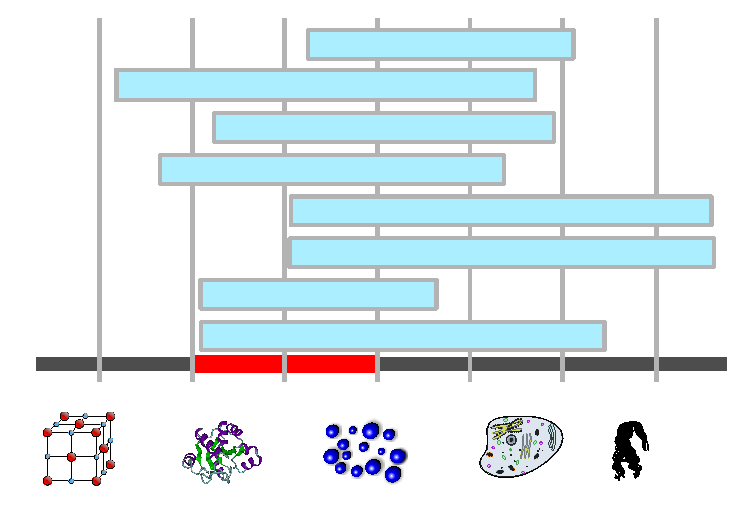
\includegraphics[width=0.95\textwidth]{Figures/SizeRange.pdf}
		\caption[Sizing techniques]{Some available sizing techniques for nanoparticles and their measuring size range.}
		\label{fig:SizeRange}
\end{figure*}

The nanoparticles envisioned for medical use are typically in the soft matter regime and thus the characterization tools must be carefully chosen considering the measurement limitations. For example, biodegradable NPs, e.g. polymeric colloids, are finding many medical applications, especially as drug-carriers \citep{kattan_phase_1992,vicent_polymer_2006} and are starting to undergo clinical trials \citep{patel_polymeric_2012,beija_colloidal_2012,cabral_progress_2014}. However, the size determination of polymeric NPs with a well-known technique like AFM is rather challenging due to their elastic properties \citep{wu_particle_2014} and suggests alternative approaches.

Liposomes are spherical vesicles composed of a closed phospholipid bilayer membrane capable of encapsulating hydrophilic compounds. The importance of lipid vesicles in the progress of nanomedicine is indisputable, as the first approved nano-drug is a liposomal formulation of doxorubicin, Doxil. Nowadays liposomes continue to be a widespread instrument for drug delivery \citep{perez-herrero_advanced_2015}, but their complicated internal structure requires typically more than a single a characterization tool \citep{khorasani_closing_2014}. Likewise, relevant biological structures in nanomedicine possess heterogeneous morphologies which are rather difficult to detect with imaging techniques \citep{baumstark_structure_1990,varga_closer_2010}. For instance, electron microscopy is an effective tool for direct observation of the shape and size distribution of nanoparticles, but it cannot conclusively elucidate their inner composition.

The use of an ensemble-averaged and non-destructive technique such as small-angle X-ray scattering (SAXS) reveals as an appropriate alternative \citep{leonard_jr_size_1952,motzkus_untersuchung_1959}. This technique can discern electron density differences in the structure of NPs and offers advantages over other methods which require prior treatment of the sample and are not averaging. SAXS is based on the elastic scattering of X-ray photons by the electron density distribution of an object and is traceable down to the SI unit \emph{m} for the size determination of sufficiently monodisperse NPs \citep{meli_traceable_2012}. The traceability of SAXS arises from the precise determination of the oscillation period on the momentum transfer axis, which is calibrated using SI traceable values of the X-ray wavelength and the scattering angle \citep{krumrey_synchrotron_2011}.

The first SAXS phenomena were observed in the 1930s by P. Krishnamurti and B.E. Warren \citep{krishnamurti_saxs_1930, warren_xray_1934} while investigating colloidal suspensions and carbon black systems. The instrumental advances introduced by \cite{kratky_berechnung_1938} and \cite{guinier_dispositif_1937} sparked the interest in the technique, while the seminal work of \cite{guinier_diffraction_1939} paved the way for the development of a SAXS theoretical background by scientists like Kratky, P. Debye or G. Porod \citep{kratky_bestimmung_1943,debye_scattering_1949,kratky_diffuse_1949,guinier_study_1950,guinier_small-angle_1955}. \cite{stuhrmann_elimination_1965}'s new approach to the understanding of the scattered intensity \citep{stuhrmann_elimination_1965} and the appearance of dedicated synchrotron radiation sources stimulated the scientific community to employ SAXS as a characterization tool. Since then, SAXS has been extensively employed in the characterization of polymeric colloids \citep{dingenouts_analysis_1999,chu_small-angle_2001,ballauff_analysis_2011} and its use in liposome research is also ubiquitous. For instance, it has been applied to characterize the lamellarity, bilayer thickness, area per lipid ratio \citep{pabst_applications_2010,bouwstra_small_1993,brzustowicz_x-ray_2005} and the thickness of the PEG-layer of different liposomal samples \citep{varga_closer_2010,varga_characterization_2012}, as well as to describe the influence of extrusion on the average number of bilayers \citep{jousma_characterization_1987} and to determine the electron density profile of liposomes \citep{bouwstra_small_1993,brzustowicz_x-ray_2005,hirai_determination_2003} and biological vesicles \citep{castorph_structure_2010}.

Despite being a highly informative method for the accurate characterization of NPs, the difficulties in the interpretation of the scattering curves in the reciprocal space asks for complementary experimental information \citep{mykhaylyk_structural_2012}. The solvent contrast variation approach is a noteworthy candidate due to the complementary data that can be collected at each independent contrast. The contrast variation method in SAXS varies systematically the electron density of the suspending medium by adding a suitable contrast agent, e.g. sucrose, in order to resolve the different contributions of the particle components to the scattering. By measuring SAXS patterns as a function of the adjusted contrast, a more detailed insight into the particle morphology can be obtained in comparison to single-contrast experiments \citep{bolze_situ_2004}. For instance, the internal structure can be modelled in terms of the radial electron density \citep{dingenouts_radial_1994,dingenouts_analysis_1999,ballauff_analysis_2011,ballauff_small-angle_1996} and the individual contribution of each component can be distinguished \citep{beyer_saxs_1990,grunder_analysis_1991,grunder_small-angle_1993,ottewill_characterization_1995,bolze_small-angle_1997,dingenouts_structure_1994} as well as its density \citep{mykhaylyk_application_2007}.

This work proposes a novel approach to solvent contrast variation in SAXS, based on the formation of a solvent density gradient within a capillary which enables the acquisition of SAXS patterns at a continuous range of contrasts, and, as a result, collect an extensive data set of complementary scattering curves in a relatively short timespan. This intelligent strategy averts the most problematic issues of the classical solvent contrast variation technique, namely the discrete range of available solvent electron densities and the prolonged time required for the preparation of the complementary samples and for obtaining the experimental data. Besides, the possibility to choose during the experiment the most appropriate contrast within the available range allows to tune \emph{in situ} the performance of the contrast variation technique in SAXS without \emph{a priori} knowledge of the investigated nanoparticles.

The structure of this thesis builds organically around the main concept presented in this work, i.e. the contrast variation technique in SAXS by means of a solvent density gradient capillary, as schematically shown in figure \ref{fig:ThesisStructure}. Following this introductory chapter, chapter \ref{chap:theory_SAXS} is dedicated to describe the theoretical framework required to understand the contrast variation method in small-angle X-ray scattering. The instrumentation employed to obtain the experimental results presented in this work is thoroughly described in chapter \ref{chap:experimental_setup}. These two chapters serve as the necessary building blocks for the development of the continuous contrast variation method based on the idea of a density gradient column. The detailed review of its performance is presented in chapter \ref{chap:density_gradient_SAXS}, where the technique is used to characterize low-density nanoparticles. The metrological possibilities of the newly introduced method are further evaluated in chapter \ref{chap:simultaneous_size_density}, focusing principally in its ability to determine the size and density of polymeric NPs in a traceable way. Finally, the scope of the technique is investigated in chapter \ref{chap:bio_applications} by using the continuous contrast variation method in a myriad of relevant nanomaterials related to nanomedicine or human biology. A last chapter \ref{chap:conclusions} acts as the necessary summary of the results presented in this work and comprises some conclusive remarks to this thesis. Extensive parts of the work presented in chapters \ref{chap:density_gradient_SAXS} to \ref{chap:bio_applications} have been published in peer-reviewed journals \citep{minelli_characterization_2014,garcia-diez_nanoparticle_2015,garcia-diez_size_2016,garcia-diez_simultaneous_2016-1}.

\begin{figure}[hbt]%[htbp]
	\centering
%%%%%%	        \def\svgwidth{0.75\linewidth}
		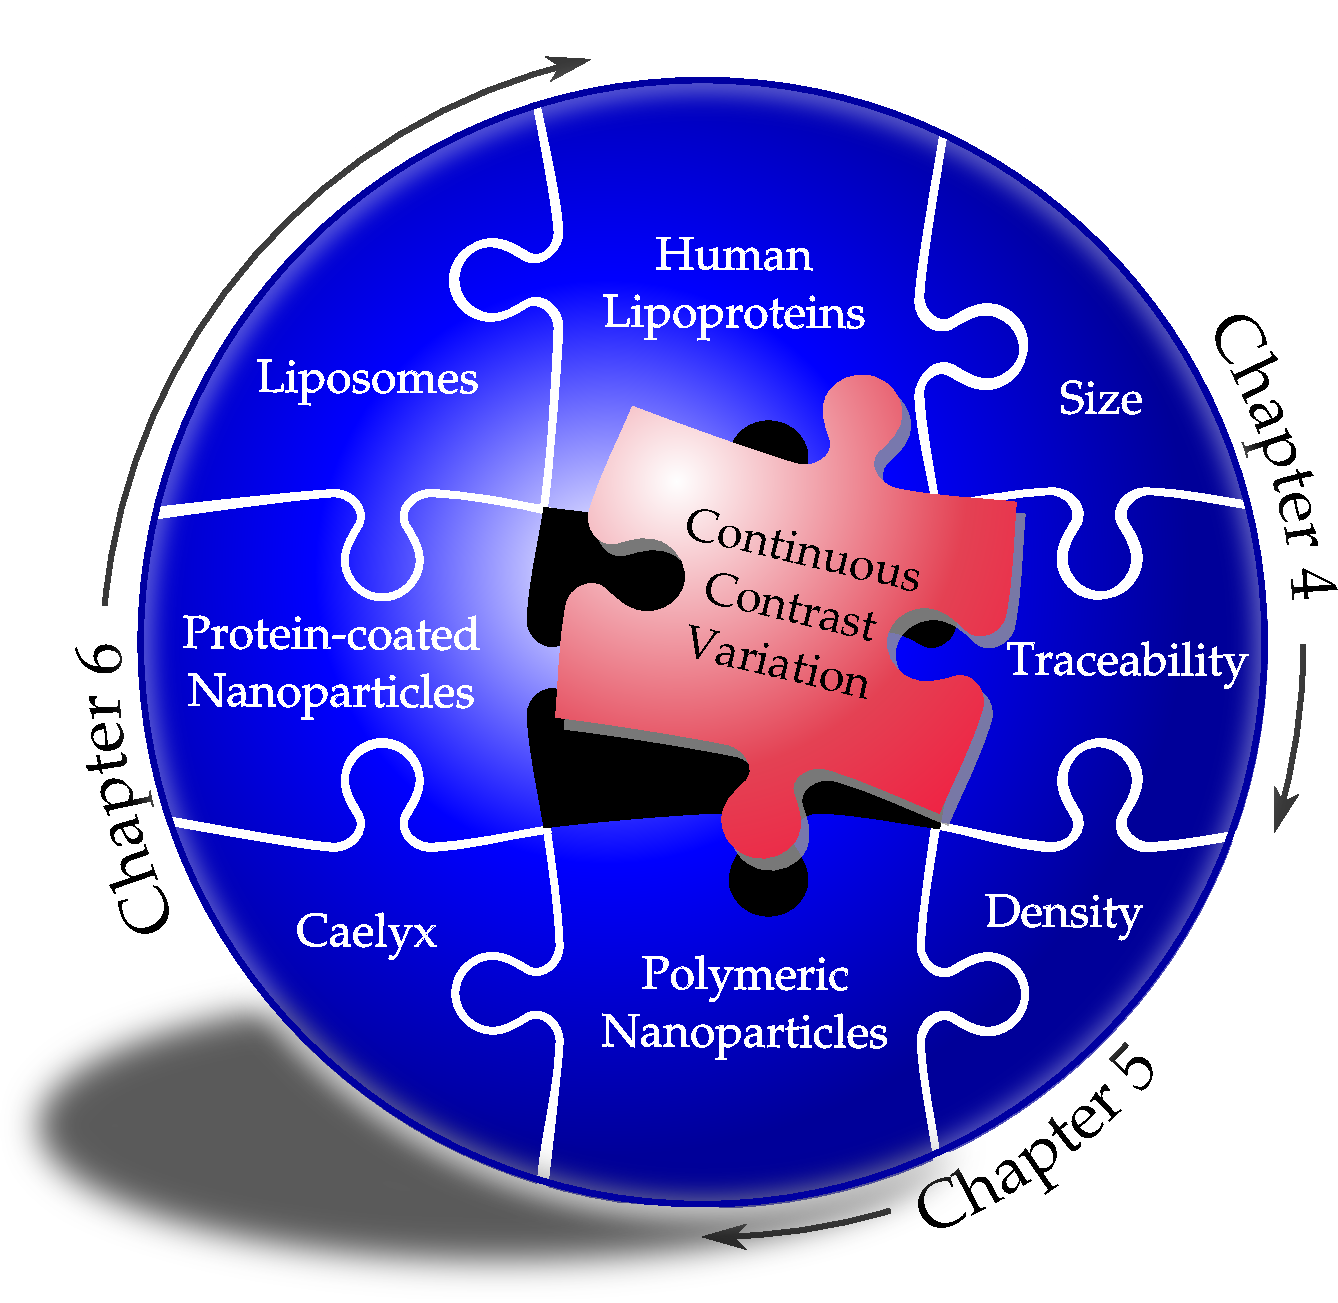
\includegraphics[width=0.65\textwidth]{Figures/ThesisStructure.pdf}
		\caption[Structure of the thesis]{Chapter structure of the work presented in this thesis. \textcolor{red}{IF THE IDEA IS GOOD, I WILL IMPROVE THE IMAGE.}}
		\label{fig:ThesisStructure}
\end{figure}


%The structure of this work feels organic, as depicted by the diagram in figure .




	
	\chapter{Theoretical Background}
\label{chap:theory_SAXS}
In this chapter, the basic physical principles underlying the operation of small-angle X-ray scattering are presented, focusing principally on the interaction between X-rays and matter and the elastic scattering of X-rays by an ensemble of electrons. The fundamental theoretical background of SAXS is also introduced, jointly with the analytical expressions of the form factors used in this work. An entire section is devoted to the theoretical framework used in contrast variation experiments in SAXS, where concepts such as the isoscattering point and the basic functions approach are introduced.

\section{Interaction of X-rays and matter}

X-rays are electromagnetic waves which propagate in vacuum along the direction of the wavevector $\vect{k}$. The incident X-ray radiation can be described by the wave function of a monochromatic plane wave:

\begin{equation}
        \label{eq:IncidentWave}
        \Psi_0\left( \vect{r} \right)=A_0 e^{i \vect{k}\vect{r} }
\end{equation}

where the wavenumber $k=\abs{\vect{k}}$ is related to the X-ray wavelength $\lambda$ by $k=\sfrac{2\pi}{\lambda}$. Conventionally, X-ray wavelengths range between 0.01 and a few nanometres, although SAXS experiments are conducted normally at the hard X-ray range, e.g. at wavelenghts between 0.02 and 0.8 nm. Due to the wave-particle duality of electromagnetic radiation, X-rays possess a particle nature as well, represented by the quantization of light into an ensemble of photons with an energy $\hbar \omega$. The photon energy is related to the X-ray wavelength by \citep{als-nielsen_elements_2011}

\begin{equation}
        \lambda = \frac{h c}{E_{ph}}
\end{equation}

where $h$ is the Planck's constant and $c$ is the speed of light in vacuum. The photon energies employed typically in SAXS experiments stretch between the silicon K-edge at 1.7 keV and some dozens of keV, including the classic copper K$_{\alpha}$ emission line at 8 keV.

\begin{figure}[hbt]%[htbp]
	\centering
	        \def\svgwidth{0.8\linewidth}
		\input{Figures/BeerLambertScheme.pdf_tex}
		\caption[Depiction of the Beer-Lambert law.]{The Beer-Lambert law is schematically depicted: The attenuation of X-rays through a medium of thickness $d$ and attenuation coefficient $\mu$ behaves accordingly to the expression \ref{eq:BeerLambertLaw}.}
		\label{fig:BeerLambertScheme}
\end{figure}


\subsection{Beer-Lambert law}
\label{sec:BeerLambert}

The interaction of X-ray photons and matter produce an attenuation of the incident radiation intensity $I_0$ which is related to the properties and volume of the material. The decrease of the intensity through a medium is schematically depicted in figure \ref{fig:BeerLambertScheme} and described by the Beer-Lambert law \citep{als-nielsen_elements_2011}:

\begin{equation}
        \label{eq:BeerLambertLaw}
        I\left( x \right)=I_0e^{-\mu x}
\end{equation}

where $\mu$ is the linear attenuation coefficient and $x$ is the radiation path length. The attenuation coefficient is dependent on the material composition and the photon energy and is directly related to the extinction coefficient $\beta$, e.g. the imaginary part of the refraction index $n$, by \citep{marr_handbook_1987}

\begin{equation}
        \mu (E) = \frac{4\pi}{hc} E \beta(E)
\end{equation}

Considering that the refractive index is expressed generally by $n = 1 - \delta +i \beta$ and $\delta<10^{-3}$ in the X-ray regime \citep{henke_x-ray_1993}, refraction effects can be neglected in scattering experiments because $\Re(n)$ is very close but smaller than unity.

When the attenuating medium is composed of different atomic species, $\mu$ can be expressed as the summation of each component attenuation coefficient $\mu_i$:

\begin{equation}
        \label{eq:AttenuationMultiComponent}
        \mu = \sum_i \mu^i = \sum_i \rho_e^i \sigma^i  =N_A\sum_i  \frac{Z^i}{A^i} \rho^i \sigma^i
\end{equation}

where $N_A$ is the Avogadro constant, $\sigma$ is the attenuation cross-section and $\rho_e$ is the number density of absorbing centres. The cross-section $\sigma$ is defined as the effective area in which photon-matter events occur. In the X-ray regime, photons interact principally with the atomic electrons, thus $\rho_e$ is the electron density and is directly proportional to the atomic number $Z$, the atomic mass number $A$ and the mass density $\rho$ of the component $i$. 

In fact, the attenuation cross-section $\sigma$ is dependent upon the several different mechanisms in which a X-ray photon interacts with the atomic electrons. The 3 most relevant effects are the photoelectron absorption, the coherent scattering and the incoherent scattering, which sum up to the total attenuation coefficient:

\begin{equation}
        \mu = \rho_e (\tau_{\text{abs}}+\sigma_{\text{scat, coh}}+\sigma_{\text{scat, incoh}})
\end{equation}

When the X-ray photon is completely absorbed by the atom, the event is called photoelectron absorption because a photoelectron with the excess energy is expelled from an inner atomic shell, leaving the atom ionized. The created core-hole is consequently filled by an electron from an outer shell either by a radiative process, i.e. \emph{fluorescence}, or by a non-radiative mechanism emitting a secondary electron, i.e. \emph{Auger effect}. The photoelectric effect is the predominant contribution to the attenuation cross-section principally at low X-ray energies and the ultraviolet regime, as shown in figure \ref{fig:AttenuationWater}. 

\begin{figure}%[htbp]
	\centering
		% GNUPLOT: LaTeX picture with Postscript
\begingroup
  \makeatletter
  \providecommand\color[2][]{%
    \GenericError{(gnuplot) \space\space\space\@spaces}{%
      Package color not loaded in conjunction with
      terminal option `colourtext'%
    }{See the gnuplot documentation for explanation.%
    }{Either use 'blacktext' in gnuplot or load the package
      color.sty in LaTeX.}%
    \renewcommand\color[2][]{}%
  }%
  \providecommand\includegraphics[2][]{%
    \GenericError{(gnuplot) \space\space\space\@spaces}{%
      Package graphicx or graphics not loaded%
    }{See the gnuplot documentation for explanation.%
    }{The gnuplot epslatex terminal needs graphicx.sty or graphics.sty.}%
    \renewcommand\includegraphics[2][]{}%
  }%
  \providecommand\rotatebox[2]{#2}%
  \@ifundefined{ifGPcolor}{%
    \newif\ifGPcolor
    \GPcolortrue
  }{}%
  \@ifundefined{ifGPblacktext}{%
    \newif\ifGPblacktext
    \GPblacktextfalse
  }{}%
  % define a \g@addto@macro without @ in the name:
  \let\gplgaddtomacro\g@addto@macro
  % define empty templates for all commands taking text:
  \gdef\gplbacktext{}%
  \gdef\gplfronttext{}%
  \makeatother
  \ifGPblacktext
    % no textcolor at all
    \def\colorrgb#1{}%
    \def\colorgray#1{}%
  \else
    % gray or color?
    \ifGPcolor
      \def\colorrgb#1{\color[rgb]{#1}}%
      \def\colorgray#1{\color[gray]{#1}}%
      \expandafter\def\csname LTw\endcsname{\color{white}}%
      \expandafter\def\csname LTb\endcsname{\color{black}}%
      \expandafter\def\csname LTa\endcsname{\color{black}}%
      \expandafter\def\csname LT0\endcsname{\color[rgb]{1,0,0}}%
      \expandafter\def\csname LT1\endcsname{\color[rgb]{0,1,0}}%
      \expandafter\def\csname LT2\endcsname{\color[rgb]{0,0,1}}%
      \expandafter\def\csname LT3\endcsname{\color[rgb]{1,0,1}}%
      \expandafter\def\csname LT4\endcsname{\color[rgb]{0,1,1}}%
      \expandafter\def\csname LT5\endcsname{\color[rgb]{1,1,0}}%
      \expandafter\def\csname LT6\endcsname{\color[rgb]{0,0,0}}%
      \expandafter\def\csname LT7\endcsname{\color[rgb]{1,0.3,0}}%
      \expandafter\def\csname LT8\endcsname{\color[rgb]{0.5,0.5,0.5}}%
    \else
      % gray
      \def\colorrgb#1{\color{black}}%
      \def\colorgray#1{\color[gray]{#1}}%
      \expandafter\def\csname LTw\endcsname{\color{white}}%
      \expandafter\def\csname LTb\endcsname{\color{black}}%
      \expandafter\def\csname LTa\endcsname{\color{black}}%
      \expandafter\def\csname LT0\endcsname{\color{black}}%
      \expandafter\def\csname LT1\endcsname{\color{black}}%
      \expandafter\def\csname LT2\endcsname{\color{black}}%
      \expandafter\def\csname LT3\endcsname{\color{black}}%
      \expandafter\def\csname LT4\endcsname{\color{black}}%
      \expandafter\def\csname LT5\endcsname{\color{black}}%
      \expandafter\def\csname LT6\endcsname{\color{black}}%
      \expandafter\def\csname LT7\endcsname{\color{black}}%
      \expandafter\def\csname LT8\endcsname{\color{black}}%
    \fi
  \fi
  \setlength{\unitlength}{0.0500bp}%
  \begin{picture}(5668.00,4534.00)%
    \gplgaddtomacro\gplbacktext{%
      \csname LTb\endcsname%
      \put(748,704){\makebox(0,0)[r]{\strut{}$10^{-6}$}}%
      \csname LTb\endcsname%
      \put(748,1061){\makebox(0,0)[r]{\strut{}$10^{-5}$}}%
      \csname LTb\endcsname%
      \put(748,1417){\makebox(0,0)[r]{\strut{}$10^{-4}$}}%
      \csname LTb\endcsname%
      \put(748,1774){\makebox(0,0)[r]{\strut{}$10^{-3}$}}%
      \csname LTb\endcsname%
      \put(748,2130){\makebox(0,0)[r]{\strut{}$10^{-2}$}}%
      \csname LTb\endcsname%
      \put(748,2487){\makebox(0,0)[r]{\strut{}$10^{-1}$}}%
      \csname LTb\endcsname%
      \put(748,2843){\makebox(0,0)[r]{\strut{}$10^{0}$}}%
      \csname LTb\endcsname%
      \put(748,3200){\makebox(0,0)[r]{\strut{}$10^{1}$}}%
      \csname LTb\endcsname%
      \put(748,3556){\makebox(0,0)[r]{\strut{}$10^{2}$}}%
      \csname LTb\endcsname%
      \put(748,3913){\makebox(0,0)[r]{\strut{}$10^{3}$}}%
      \csname LTb\endcsname%
      \put(748,4269){\makebox(0,0)[r]{\strut{}$10^{4}$}}%
      \csname LTb\endcsname%
      \put(880,484){\makebox(0,0){\strut{} 1}}%
      \csname LTb\endcsname%
      \put(2344,484){\makebox(0,0){\strut{} 10}}%
      \csname LTb\endcsname%
      \put(3807,484){\makebox(0,0){\strut{} 100}}%
      \csname LTb\endcsname%
      \put(5271,484){\makebox(0,0){\strut{} 1000}}%
      \put(176,2486){\rotatebox{-270}{\makebox(0,0){\strut{}Water attenuation / cm$^{-1}$}}}%
      \put(3075,154){\makebox(0,0){\strut{}Photon Energy / keV}}%
    }%
    \gplgaddtomacro\gplfronttext{%
      \csname LTb\endcsname%
      \put(4548,4096){\makebox(0,0)[r]{\strut{}\smaller Photoelectron Absorption}}%
      \csname LTb\endcsname%
      \put(4548,3876){\makebox(0,0)[r]{\strut{}\smaller Coherent Scattering}}%
      \csname LTb\endcsname%
      \put(4548,3656){\makebox(0,0)[r]{\strut{}\smaller Incoherent Scattering}}%
    }%
    \gplbacktext
    \put(0,0){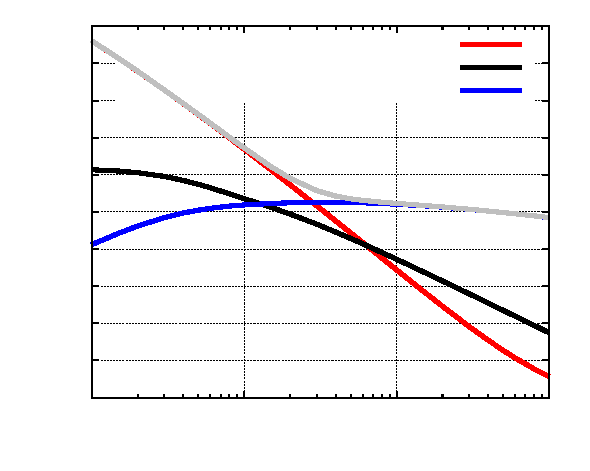
\includegraphics{AttenuationWater}}%
    \gplfronttext
  \end{picture}%
\endgroup

		\caption[Contributions to the X-ray attenuation coefficient of water.]{The different contributions to the attenuation of water at room temperature are depicted as a function of the photon energy \citep{henke_x-ray_1993} and the total attenuation is the summation of all the other contributions. The pair production in nuclear and electron field can be neglected at the displayed photon energies.}
		\label{fig:AttenuationWater}
\end{figure}

The other relevant contributions in the X-ray range are related to scattering processes. In an inelastic scattering event, the energy of the incident photon is partially transfered to a loosely bound electron resulting in a scattered photon with a longer wavelength, according to the Compton relation $\Delta\lambda = \sfrac{h}{m_e c}\left( 1 - \cos{2\theta} \right) $ \citep{als-nielsen_elements_2011}, where $2\theta$ is the scattering angle. The Compton scattering is incoherent and contributes generally less than the elastic scattering at energies below 10 keV, as observed in figure \ref{fig:AttenuationWater}. Besides, the coherent scattering signal is the summation of the constructive interferences of the electromagnetic wave, which produces a higher scattering intensity than the inelastic scattering. In fact, the elastic scattering of X-rays, typically coherent, is the main process used in material investigations and the physical principle behind SAXS.

\subsection{Elastic scattering}
\label{sec:ElasticScattering}

When the wavelength of the scattered wave is the same than that of the incident one, the proccess is named elastic scattering or coherent scattering and the resulting intensity is the absolute square of the sum of the scattering amplitudes. In the following sections, the elastic scattering theory will be presented for the classical case and for an ensemble of electrons.

\subsubsection{Thomson scattering}

\begin{figure}%[htbp]
\centering
\def\svgwidth{0.95\linewidth}
\input{Figures/FraunhoferScheme.pdf_tex}
\caption[Schematics of a scattering process and graphical definition of $\vect{q}$.]{Scheme of an scattering event by an object with a potential function $\phi(\vect{r'})$ at a distance $\abs{\vect{r}}=r$. A geometrical definition of the momentum transfer vector $\vect{q}$ is depicted on the right hand side, where $\vect{k}$ and $\vect{k_s}$ are the incident and scattered wavevector respectively.}
\label{fig:FraunhoferScheme}
\end{figure}

Classically, the elastic scattering of a photon by a free electron is described by the conservation of the photon energy, i.e. the wavenumber of the scattered wave is the same than the incident one ($\abs{\vect{k_s}}=\abs{\vect{k}}$). Consequently for unpolarized incident radiation, the intensity of the scattered wave at a distance $r$ and with a scattering angle $2\theta$ is defined by \citep{warren_x-ray_1969}:

\begin{equation}
        I_{\text{scat}}\left( r,\theta \right)= I_0 \left( \frac{r_e}{r} \right) ^2 \left( \frac{1+\cos^2{2\theta}}{2} \right)
\end{equation}

where $r_e= \sfrac{e^2}{4\pi\epsilon_0 m_e c^2}=2.82\cdot10^{-15}$ m is the Thomson or classical electron radius. A relevant quantity in scattering processes is the differential scattering cross-section $\sfrac{d\sigma}{d\Omega}$, which is directly proportional to the scattering intensity $I_{\text{scat}}$. It is defined as the the number of scattered photons per time and per solid angle over the incident intensity per time and per area \citep{als-nielsen_elements_2011}:

\begin{equation}
        \label{eq:thomson_cross_section}
        \frac{d\sigma}{d\Omega}= \frac{I_{\text{scat}} \cdot \left(r^2 \Delta \Omega \right)}{I_0\Delta \Omega}=r_e^2\left( \frac{1+\cos^2{2\theta}}{2} \right)
\end{equation}

where $r^2 \Delta \Omega$ is the detector surface in the plane of the impact parameter. The total Thomson scattering cross-section is $\sigma = \sfrac{8\pi r_0^2}{3} = 0.665\cdot10^{-24}$ cm$^2$ and similarly to $\sfrac{d\sigma}{d\Omega}$ is proportional to $r_e^2$ and independent from the photon energy if the photon wavelength is distant of an X-ray absorption edge.

\subsubsection{Scattering by an ensemble of electrons}

The scattering of a photon by an ensemble of weakly bound electrons can be studied by considering the interaction of particles with a three-dimensional weak potential $V(\vect{r})=V_0 \cdot \phi(\vect{r})$, where $V_0$ is the strength of the potential and $\phi(\vect{r})$ is the so-called \emph{potential function}. The resulting wave can be expressed as a linear combination of the incident plane wave (see equation \ref{eq:IncidentWave}) and the scattered spherical wave at the position $\vect{r}$:

\begin{equation}
       \Psi\left( \vect{r} \right)= \Psi_0\left( \vect{r} \right) +  \Psi_{\text{scat}}\left( \vect{r} \right)
\end{equation}

Inserting this expression at the time-independent Schrödinger equation and considering the scattering wave as a perturbation produced by the scattering potential function $\phi(\vect{r})$ \citep{cowley_diffraction_1995}, it can be derived that

\begin{equation}
       \Psi_{\text{scat}}\left( \vect{r} \right)=C \int \frac{e^{ i k\abs{\vect{r}-\vect{r}'} } } {\abs{\vect{r}-\vect{r}'}} \phi(\vect{r}')   \Psi\left( \vect{r}' \right) d\vect{r}'^3
\end{equation}

where $C$ is the so-called \emph{scattering length}. If the detection position $\vect{r}$ is at distance much larger than the scattering object size, as outlined in figure \ref{fig:FraunhoferScheme}, the Fraunhofer approximation applies and $\abs{\vect{r}-\vect{r'}} \simeq r$ \citep{feigin_structure_1987}, resulting in

\begin{equation}
       \Psi_{\text{scat}}\left( \vect{r} \right)=C \frac{e^{i k r}}{r} \int e^{ -i \vect{k}\vect{r}' }  \phi(\vect{r}')   \Psi\left( \vect{r}' \right) d\vect{r}'^3
\end{equation}

Assuming that there are no multiple scattering events due to the low concentration of scatterers and that the interaction potential is weak, the first Born approximation can be employed ($ \Psi\left( \vect{r} \right) \simeq \Psi_0\left( \vect{r} \right)$) \citep{cowley_diffraction_1995}, leading to

\begin{equation}
       \Psi_{\text{scat}}\left( \vect{r} \right)=C A_0 \frac{e^{i k r}}{r} \int e^{ i \vect{q}\vect{r}' }  \phi(\vect{r}')  d\vect{r}'^3
\end{equation}

where $\vect{q}=\vect{k_s} - \vect{k}$ is the momentum transfer vector and $\vect{k_s}$ the scattered wavevector. Analogously to equation \ref{eq:thomson_cross_section}, the differential scattering cross-section is:

\begin{equation}
        \label{eq:rayleigh_cross_section}
\frac{d\sigma}{d\Omega}= \frac{\abs{\Psi_{\text{scat}}}^2 \cdot \left(r^2 \Delta \Omega \right)}{\abs{\Psi_{0}}^2\Delta \Omega}=r_e^2 \abs{f(\vect{q})}^2 =r_e^2 \; I(\vect{q})
\end{equation}

where $f(\vect{q})=\int e^{ i \vect{q}\vect{r}' }  \phi(\vect{r}')  d\vect{r}'^3$ is the scattering amplitude, $I(\vect{q}) = \abs{f(\vect{q})}^2$ is the scattering intensity and the scattering length is the classical electron radius $r_e$. The scattering amplitude  $f(\vect{q})$ is simply the Fourier transform of the scattering potential function $\phi(\vect{r})$.

This type of scattering mechanism is named Rayleigh-Gans-Debye when the refractive index of the object $n_{\text{obj}}$ is close to unity and the condition $\sfrac{2\pi}{\lambda} \cdot D \cdot  \abs{n_{\text{med}} - n_{\text{obj}}} \ll 1$ is fulfilled, being $D$ the size of the object and $n_{\text{med}}$ the refractive index of the suspending medium. For X-ray photons with wavelenghts $\lambda$ around 0.1 nm and nanoscaled objects, this approximation can be applied and it can be safely assumed that the same electromagnetic wave impinges each part of the object \citep{hulst_light_1957, barber_rayleigh-gans-debye_1978}. In the case of optical radiation scattered by colloids, the Mie scattering framework is used, while the Rayleigh scattering corresponds to light wavelengths much larger than the scattering object.

\subsubsection{Anomalous scattering}

In X-ray scattering experiments, the scattering centres are the electrons of the atom and the scattering potential function is the electron charge density about the nucleous, so $\phi(\vect{r})=\rho_e(\vect{r})$. The electron density is related to the atomic properties as introduced in equation \ref{eq:AttenuationMultiComponent} and therefore the scattering amplitude increases with the atomic number $Z$ as can be shown by calculating equation \ref{eq:rayleigh_cross_section} at the limit $\vect{q} \rightarrow 0$

\begin{equation}
        f(\vect{q} \rightarrow 0) = \int \rho_e(\vect{r}')  d\vect{r}'^3 = Z
\end{equation}

This is valid when the incident photon energy is much larger than the energy corresponding to a resonant excitation. When the X-ray energy is close to an absorption edge, the anomalous dispersion becomes relevant and the scattering amplitude depends on the energy of the X-ray by adding the anomalous corrections \citep{als-nielsen_elements_2011}:

\begin{equation}
        f(E) = f_0 + f'(E) + i f'' (E)
\end{equation}

where the imaginary part $f''$ is related to the attenuation coefficient $\mu$ by \citep{feigin_structure_1987}

\begin{equation}
        f'' (E) = \frac{A\rho}{2N_A r_e h c} E \mu(E)
\end{equation}

where $A$ is the atomic mass of the resonant atom and $\rho$ its mass density. The term $f'$ is related to the imaginary anomalous coefficient by the Kramers-Kronig relationship \citep{de_l._kronig_theory_1926,kramers_diffusion_1927}:

\begin{equation}
        f'(E) = \frac{2}{\pi} \int_0^{\infty} \frac{E'f''(E')dE'}{E^2 - E'^2}
\end{equation}

The values of the anomalous scattering amplitude $f(E)$ are usually calculated using the experimentally measured attenuation coefficient $\mu(E)$.

\section{Small-angle X-ray scattering}
\label{sec:SAXS_theory}

Small-angle X-ray scattering is a powerful technique that can elucidate the structural features of particles with sizes ranging from a few nanometres up to some hundreds of nanometres. By investigating the photons elastically scattered by the electron density distribution of the particle $\rho_e ( \vect{r} )$, the resulting patterns can be analysed employing equation \ref{eq:rayleigh_cross_section} to obtain information about the particle size, shape and composition. Two fundamental quantities in a SAXS experiment are the scattering intensity $I(\vect{q})$, proportional to $\sfrac{d\sigma}{d\Omega}$, and the scattering amplitude or \emph{form factor} $f(\vect{q})$. The latter is expressed for objects with spherical symmetry where $\rho_e(\vect{r})=\rho_e(r)$ by

\begin{equation}
        \label{eq:FormFactorSpherical}
        f(q)=4\pi \int_0^{\infty} r'^2 \rho_e(r')  \frac{\sin(qr')}{qr'}  dr'
\end{equation}

where the modulus of the momentum transfer vector is defined by $q=\abs{\vect{q}}=\abs{\vect{k_s} - \vect{k}}$. Considering that SAXS is an elastic scattering process ($\abs{\vect{k_s}}=\abs{\vect{k}}=\sfrac{2\pi}{\lambda}$), the momentum transfer is expressed as

\begin{equation}
q=\frac{4\pi }{\lambda}\sin\theta=\frac{4\pi E}{h c}\sin\theta ,
\end{equation}

where \(\theta\) is half of the scattering angle as depicted in figure \ref{fig:FraunhoferScheme}, \(h\) is the Planck constant and \(c\) is the speed of light.

The systems studied by SAXS in this work consist of particles suspended in a uniform medium, e.g. water or buffer, with a different electron density $\rho_{\text{medium}}$ than the studied particle. In fact, the measured scattering amplitude is the addition of the medium and the particle contributions. Therefore, the scattering of the studied object is expressed in terms of the \emph{contrast}, $\Delta \eta (\vect{r}) = \rho_e(\vect{r}) - \rho_{\text{medium}}$, the electron density difference between the particle and the embedded matrix or surrounding medium. This leads to a slight modification of equation \ref{eq:FormFactorSpherical}, where $\rho_e(r)$ can be substituted by the contrast $\Delta\eta(r)$ to distinguish the contribution of the investigated particle from that of the medium.

\subsection{Scattering by an ensemble of particles}

For diluted systems with low particle concentration, the wave scattered by a particle does not interfere coherently with the neighboring particles, hence the scattering intensity can be expressed as a sum of the scattering of the individual particles, i.e. the structure factor contribution can be neglected because $S(q)=1$ \citep{feigin_structure_1987}. Assuming this premise, the scattering intensity of an ensemble of randomly oriented spherically symmetric nanoparticles in a diluted suspension can be expressed as

\begin{equation}
\label{eq:intensity}
I(q)=N\int_{0}^{\infty} g(R)\left|f(q,R) \right|^2 dR,
\end{equation}

where \(N\) is the number of scatterers i.e particles, \(g(R)\) is their size distribution function and \(f(q,R)\) is the particle form factor, which depends on the radial structure of the particle as determined in equation \ref{eq:FormFactorSpherical}. Generally, the particles in suspension are not monodisperse and show a certain size distribution which is often related with their chemical preparation. For systems of relatively low size polydispersity, a gaussian size distribution is typically a good choice, which is expressed by:

\begin{equation}
        \label{eq:gauss_distribution}
       g_{\text{Gauss}}(R)=\frac{1}{\sigma_R \sqrt{2\pi}} e^{ - \frac{\left( R - \overline{R} \right)^2}{2\sigma_R^2} }
\end{equation}

where $\overline{R}$ is the mean radius of the particles and $\sigma_R$ is the standard deviation of the size distribution. For smaller particles or higher polydispersity degrees, a log-normal distribution is preferred, defined as

\begin{equation}
       g_{\text{LN}}(R)=\frac{1}{\sigma_R \sqrt{2\pi}} e^{ - \frac{\left( \ln(R) - \ln(\overline{R}) \right)^2}{2\sigma_R^2} }
\end{equation}

whose mean radius is given by $\overline{R} e^{\frac{\sigma_R^2}{2}}$ and the variance is $\overline{R}^2 e^{\sigma_R^2} (e^{\sigma_R^2} - 1)$. Other approaches to the size distribution of particles in solution are based in numerical techniques, like the Monte-Carlo approach to form-free particle size distributions \citep{pauw_improvements_2013}.

A useful parameter for comparative purposes between samples is the polydispersity degree $p_d$, which is defined as the full width at half maximum (FWHM) of the number-weighted particle size distribution divided by its average value. For a normal size distribution, the FWHM is simply $8\sqrt{2}$ times its standard deviation $\sigma_R$.

\subsection{The scattering curve}

The differential scattering cross-section $\sfrac{d\sigma}{d\Omega}$ is the fundamental measurand in a SAXS experiment, as described in section \ref{sec:ElasticScattering}. Nevertheless, some comparability challenges arise from this quantity as it depends on the sample volume $V$ used in the experiment. This can be solved by introducing the differential scattering cross-section per volume, historically given in cm$^{-1}$. The expression of this quantity is derived from equations \ref{eq:rayleigh_cross_section} and \ref{eq:intensity} and leads to:

\begin{equation}
\frac{d\Sigma}{d\Omega} (q) = \frac{\sfrac{d\sigma}{d\Omega}(q)}{V} = \frac{r_e^2 \; I(q)}{V} = r_e^2 \cdot \frac{N}{V} \cdot \int_0^{\infty} g(R) \abs{ f(q,R) }^2 dR
\end{equation}

where $\sfrac{N}{V}$ is the concentration of scatterers, i.e. particles.

%\begin{figure}
%	\centering
%        	\resizebox{.85\linewidth}{!}{% GNUPLOT: LaTeX picture with Postscript
\begingroup
  \makeatletter
  \providecommand\color[2][]{%
    \GenericError{(gnuplot) \space\space\space\@spaces}{%
      Package color not loaded in conjunction with
      terminal option `colourtext'%
    }{See the gnuplot documentation for explanation.%
    }{Either use 'blacktext' in gnuplot or load the package
      color.sty in LaTeX.}%
    \renewcommand\color[2][]{}%
  }%
  \providecommand\includegraphics[2][]{%
    \GenericError{(gnuplot) \space\space\space\@spaces}{%
      Package graphicx or graphics not loaded%
    }{See the gnuplot documentation for explanation.%
    }{The gnuplot epslatex terminal needs graphicx.sty or graphics.sty.}%
    \renewcommand\includegraphics[2][]{}%
  }%
  \providecommand\rotatebox[2]{#2}%
  \@ifundefined{ifGPcolor}{%
    \newif\ifGPcolor
    \GPcolortrue
  }{}%
  \@ifundefined{ifGPblacktext}{%
    \newif\ifGPblacktext
    \GPblacktextfalse
  }{}%
  % define a \g@addto@macro without @ in the name:
  \let\gplgaddtomacro\g@addto@macro
  % define empty templates for all commands taking text:
  \gdef\gplbacktext{}%
  \gdef\gplfronttext{}%
  \makeatother
  \ifGPblacktext
    % no textcolor at all
    \def\colorrgb#1{}%
    \def\colorgray#1{}%
  \else
    % gray or color?
    \ifGPcolor
      \def\colorrgb#1{\color[rgb]{#1}}%
      \def\colorgray#1{\color[gray]{#1}}%
      \expandafter\def\csname LTw\endcsname{\color{white}}%
      \expandafter\def\csname LTb\endcsname{\color{black}}%
      \expandafter\def\csname LTa\endcsname{\color{black}}%
      \expandafter\def\csname LT0\endcsname{\color[rgb]{1,0,0}}%
      \expandafter\def\csname LT1\endcsname{\color[rgb]{0,1,0}}%
      \expandafter\def\csname LT2\endcsname{\color[rgb]{0,0,1}}%
      \expandafter\def\csname LT3\endcsname{\color[rgb]{1,0,1}}%
      \expandafter\def\csname LT4\endcsname{\color[rgb]{0,1,1}}%
      \expandafter\def\csname LT5\endcsname{\color[rgb]{1,1,0}}%
      \expandafter\def\csname LT6\endcsname{\color[rgb]{0,0,0}}%
      \expandafter\def\csname LT7\endcsname{\color[rgb]{1,0.3,0}}%
      \expandafter\def\csname LT8\endcsname{\color[rgb]{0.5,0.5,0.5}}%
    \else
      % gray
      \def\colorrgb#1{\color{black}}%
      \def\colorgray#1{\color[gray]{#1}}%
      \expandafter\def\csname LTw\endcsname{\color{white}}%
      \expandafter\def\csname LTb\endcsname{\color{black}}%
      \expandafter\def\csname LTa\endcsname{\color{black}}%
      \expandafter\def\csname LT0\endcsname{\color{black}}%
      \expandafter\def\csname LT1\endcsname{\color{black}}%
      \expandafter\def\csname LT2\endcsname{\color{black}}%
      \expandafter\def\csname LT3\endcsname{\color{black}}%
      \expandafter\def\csname LT4\endcsname{\color{black}}%
      \expandafter\def\csname LT5\endcsname{\color{black}}%
      \expandafter\def\csname LT6\endcsname{\color{black}}%
      \expandafter\def\csname LT7\endcsname{\color{black}}%
      \expandafter\def\csname LT8\endcsname{\color{black}}%
    \fi
  \fi
    \setlength{\unitlength}{0.0500bp}%
    \ifx\gptboxheight\undefined%
      \newlength{\gptboxheight}%
      \newlength{\gptboxwidth}%
      \newsavebox{\gptboxtext}%
    \fi%
    \setlength{\fboxrule}{0.5pt}%
    \setlength{\fboxsep}{1pt}%
\begin{picture}(5668.00,4534.00)%
    \gplgaddtomacro\gplbacktext{%
    }%
    \gplgaddtomacro\gplfronttext{%
      \csname LTb\endcsname%
      \put(176,2486){\rotatebox{-270}{\makebox(0,0){\strut{}$\sfrac{d \Sigma}{d \Omega}$ / cm$^{-1}$}}}%
      \put(3108,154){\makebox(0,0){\strut{}$q$ / nm$^{-1}$}}%
      \csname LTb\endcsname%
      \put(814,704){\makebox(0,0)[r]{\strut{}$10^{-4}$}}%
      \csname LTb\endcsname%
      \put(814,1213){\makebox(0,0)[r]{\strut{}$10^{-3}$}}%
      \csname LTb\endcsname%
      \put(814,1723){\makebox(0,0)[r]{\strut{}$10^{-2}$}}%
      \csname LTb\endcsname%
      \put(814,2232){\makebox(0,0)[r]{\strut{}$10^{-1}$}}%
      \csname LTb\endcsname%
      \put(814,2741){\makebox(0,0)[r]{\strut{}$10^{0}$}}%
      \csname LTb\endcsname%
      \put(814,3250){\makebox(0,0)[r]{\strut{}$10^{1}$}}%
      \csname LTb\endcsname%
      \put(814,3760){\makebox(0,0)[r]{\strut{}$10^{2}$}}%
      \csname LTb\endcsname%
      \put(814,4269){\makebox(0,0)[r]{\strut{}$10^{3}$}}%
      \csname LTb\endcsname%
      \put(946,484){\makebox(0,0){\strut{}$0.01$}}%
      \csname LTb\endcsname%
      \put(3108,484){\makebox(0,0){\strut{}$0.1$}}%
      \csname LTb\endcsname%
      \put(5271,484){\makebox(0,0){\strut{}$1$}}%
      \put(1117,4066){\makebox(0,0)[l]{\strut{}Guinier region}}%
      \put(4521,4066){\makebox(0,0)[l]{\strut{}Porod}}%
      \put(4521,3846){\makebox(0,0)[l]{\strut{}region}}%
      \put(2911,4066){\makebox(0,0)[l]{\strut{}Fourier region}}%
    }%
    \gplbacktext
    \put(0,0){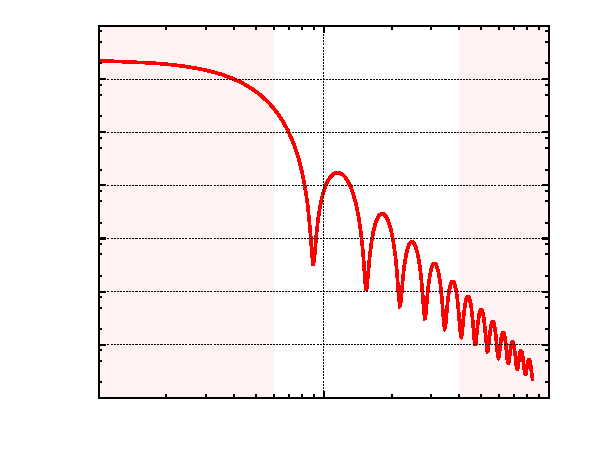
\includegraphics{ScatteringCurve50nm}}%
    \gplfronttext
  \end{picture}%
\endgroup
}
		%% GNUPLOT: LaTeX picture with Postscript
\begingroup
  \makeatletter
  \providecommand\color[2][]{%
    \GenericError{(gnuplot) \space\space\space\@spaces}{%
      Package color not loaded in conjunction with
      terminal option `colourtext'%
    }{See the gnuplot documentation for explanation.%
    }{Either use 'blacktext' in gnuplot or load the package
      color.sty in LaTeX.}%
    \renewcommand\color[2][]{}%
  }%
  \providecommand\includegraphics[2][]{%
    \GenericError{(gnuplot) \space\space\space\@spaces}{%
      Package graphicx or graphics not loaded%
    }{See the gnuplot documentation for explanation.%
    }{The gnuplot epslatex terminal needs graphicx.sty or graphics.sty.}%
    \renewcommand\includegraphics[2][]{}%
  }%
  \providecommand\rotatebox[2]{#2}%
  \@ifundefined{ifGPcolor}{%
    \newif\ifGPcolor
    \GPcolortrue
  }{}%
  \@ifundefined{ifGPblacktext}{%
    \newif\ifGPblacktext
    \GPblacktextfalse
  }{}%
  % define a \g@addto@macro without @ in the name:
  \let\gplgaddtomacro\g@addto@macro
  % define empty templates for all commands taking text:
  \gdef\gplbacktext{}%
  \gdef\gplfronttext{}%
  \makeatother
  \ifGPblacktext
    % no textcolor at all
    \def\colorrgb#1{}%
    \def\colorgray#1{}%
  \else
    % gray or color?
    \ifGPcolor
      \def\colorrgb#1{\color[rgb]{#1}}%
      \def\colorgray#1{\color[gray]{#1}}%
      \expandafter\def\csname LTw\endcsname{\color{white}}%
      \expandafter\def\csname LTb\endcsname{\color{black}}%
      \expandafter\def\csname LTa\endcsname{\color{black}}%
      \expandafter\def\csname LT0\endcsname{\color[rgb]{1,0,0}}%
      \expandafter\def\csname LT1\endcsname{\color[rgb]{0,1,0}}%
      \expandafter\def\csname LT2\endcsname{\color[rgb]{0,0,1}}%
      \expandafter\def\csname LT3\endcsname{\color[rgb]{1,0,1}}%
      \expandafter\def\csname LT4\endcsname{\color[rgb]{0,1,1}}%
      \expandafter\def\csname LT5\endcsname{\color[rgb]{1,1,0}}%
      \expandafter\def\csname LT6\endcsname{\color[rgb]{0,0,0}}%
      \expandafter\def\csname LT7\endcsname{\color[rgb]{1,0.3,0}}%
      \expandafter\def\csname LT8\endcsname{\color[rgb]{0.5,0.5,0.5}}%
    \else
      % gray
      \def\colorrgb#1{\color{black}}%
      \def\colorgray#1{\color[gray]{#1}}%
      \expandafter\def\csname LTw\endcsname{\color{white}}%
      \expandafter\def\csname LTb\endcsname{\color{black}}%
      \expandafter\def\csname LTa\endcsname{\color{black}}%
      \expandafter\def\csname LT0\endcsname{\color{black}}%
      \expandafter\def\csname LT1\endcsname{\color{black}}%
      \expandafter\def\csname LT2\endcsname{\color{black}}%
      \expandafter\def\csname LT3\endcsname{\color{black}}%
      \expandafter\def\csname LT4\endcsname{\color{black}}%
      \expandafter\def\csname LT5\endcsname{\color{black}}%
      \expandafter\def\csname LT6\endcsname{\color{black}}%
      \expandafter\def\csname LT7\endcsname{\color{black}}%
      \expandafter\def\csname LT8\endcsname{\color{black}}%
    \fi
  \fi
    \setlength{\unitlength}{0.0500bp}%
    \ifx\gptboxheight\undefined%
      \newlength{\gptboxheight}%
      \newlength{\gptboxwidth}%
      \newsavebox{\gptboxtext}%
    \fi%
    \setlength{\fboxrule}{0.5pt}%
    \setlength{\fboxsep}{1pt}%
\begin{picture}(5668.00,4534.00)%
    \gplgaddtomacro\gplbacktext{%
    }%
    \gplgaddtomacro\gplfronttext{%
      \csname LTb\endcsname%
      \put(176,2486){\rotatebox{-270}{\makebox(0,0){\strut{}$\sfrac{d \Sigma}{d \Omega}$ / cm$^{-1}$}}}%
      \put(3108,154){\makebox(0,0){\strut{}$q$ / nm$^{-1}$}}%
      \csname LTb\endcsname%
      \put(814,704){\makebox(0,0)[r]{\strut{}$10^{-4}$}}%
      \csname LTb\endcsname%
      \put(814,1213){\makebox(0,0)[r]{\strut{}$10^{-3}$}}%
      \csname LTb\endcsname%
      \put(814,1723){\makebox(0,0)[r]{\strut{}$10^{-2}$}}%
      \csname LTb\endcsname%
      \put(814,2232){\makebox(0,0)[r]{\strut{}$10^{-1}$}}%
      \csname LTb\endcsname%
      \put(814,2741){\makebox(0,0)[r]{\strut{}$10^{0}$}}%
      \csname LTb\endcsname%
      \put(814,3250){\makebox(0,0)[r]{\strut{}$10^{1}$}}%
      \csname LTb\endcsname%
      \put(814,3760){\makebox(0,0)[r]{\strut{}$10^{2}$}}%
      \csname LTb\endcsname%
      \put(814,4269){\makebox(0,0)[r]{\strut{}$10^{3}$}}%
      \csname LTb\endcsname%
      \put(946,484){\makebox(0,0){\strut{}$0.01$}}%
      \csname LTb\endcsname%
      \put(3108,484){\makebox(0,0){\strut{}$0.1$}}%
      \csname LTb\endcsname%
      \put(5271,484){\makebox(0,0){\strut{}$1$}}%
      \put(1117,4066){\makebox(0,0)[l]{\strut{}Guinier region}}%
      \put(4521,4066){\makebox(0,0)[l]{\strut{}Porod}}%
      \put(4521,3846){\makebox(0,0)[l]{\strut{}region}}%
      \put(2911,4066){\makebox(0,0)[l]{\strut{}Fourier region}}%
    }%
    \gplbacktext
    \put(0,0){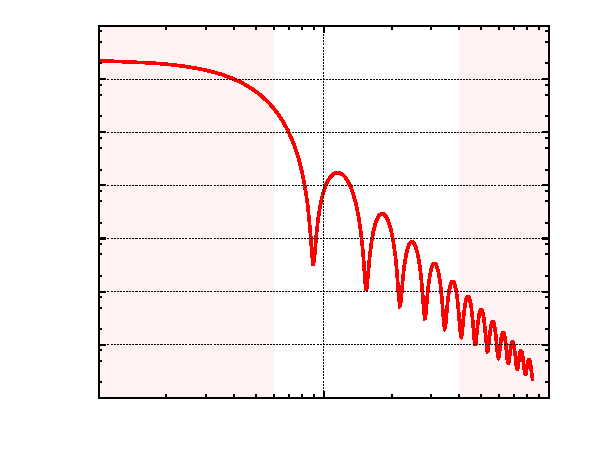
\includegraphics{ScatteringCurve50nm}}%
    \gplfronttext
  \end{picture}%
\endgroup

%		\caption[The scattering curve and its relevant regions.]{Simulated scattering curve of a nanoparticle ensemble with radius 50 nm and a polydispersity degree of 10 $\%$. The three different regions discussed in the text are highlighted in the figure as well.}
%		\label{fig:ScatteringCurve50nm}
%\end{figure}

\begin{figure*}%[htbp]
	\centering
		\subfloat[The scattering pattern]{\resizebox{0.35\linewidth}{!}{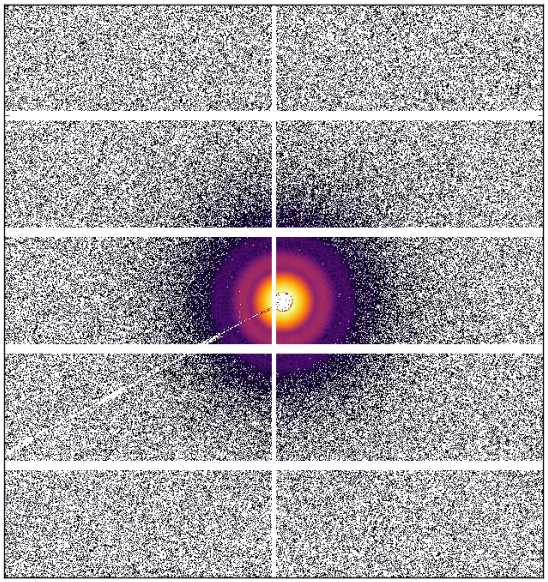
\includegraphics{Figures/Au100ScatteringPattern_edit2}}\label{fig:Au100ScatteringPattern}}
		\qquad
		\subfloat[The scattering curve and its relevant regions.]{\resizebox{0.5\linewidth}{!}{\figfont{12pt}% GNUPLOT: LaTeX picture with Postscript
\begingroup
  \makeatletter
  \providecommand\color[2][]{%
    \GenericError{(gnuplot) \space\space\space\@spaces}{%
      Package color not loaded in conjunction with
      terminal option `colourtext'%
    }{See the gnuplot documentation for explanation.%
    }{Either use 'blacktext' in gnuplot or load the package
      color.sty in LaTeX.}%
    \renewcommand\color[2][]{}%
  }%
  \providecommand\includegraphics[2][]{%
    \GenericError{(gnuplot) \space\space\space\@spaces}{%
      Package graphicx or graphics not loaded%
    }{See the gnuplot documentation for explanation.%
    }{The gnuplot epslatex terminal needs graphicx.sty or graphics.sty.}%
    \renewcommand\includegraphics[2][]{}%
  }%
  \providecommand\rotatebox[2]{#2}%
  \@ifundefined{ifGPcolor}{%
    \newif\ifGPcolor
    \GPcolortrue
  }{}%
  \@ifundefined{ifGPblacktext}{%
    \newif\ifGPblacktext
    \GPblacktextfalse
  }{}%
  % define a \g@addto@macro without @ in the name:
  \let\gplgaddtomacro\g@addto@macro
  % define empty templates for all commands taking text:
  \gdef\gplbacktext{}%
  \gdef\gplfronttext{}%
  \makeatother
  \ifGPblacktext
    % no textcolor at all
    \def\colorrgb#1{}%
    \def\colorgray#1{}%
  \else
    % gray or color?
    \ifGPcolor
      \def\colorrgb#1{\color[rgb]{#1}}%
      \def\colorgray#1{\color[gray]{#1}}%
      \expandafter\def\csname LTw\endcsname{\color{white}}%
      \expandafter\def\csname LTb\endcsname{\color{black}}%
      \expandafter\def\csname LTa\endcsname{\color{black}}%
      \expandafter\def\csname LT0\endcsname{\color[rgb]{1,0,0}}%
      \expandafter\def\csname LT1\endcsname{\color[rgb]{0,1,0}}%
      \expandafter\def\csname LT2\endcsname{\color[rgb]{0,0,1}}%
      \expandafter\def\csname LT3\endcsname{\color[rgb]{1,0,1}}%
      \expandafter\def\csname LT4\endcsname{\color[rgb]{0,1,1}}%
      \expandafter\def\csname LT5\endcsname{\color[rgb]{1,1,0}}%
      \expandafter\def\csname LT6\endcsname{\color[rgb]{0,0,0}}%
      \expandafter\def\csname LT7\endcsname{\color[rgb]{1,0.3,0}}%
      \expandafter\def\csname LT8\endcsname{\color[rgb]{0.5,0.5,0.5}}%
    \else
      % gray
      \def\colorrgb#1{\color{black}}%
      \def\colorgray#1{\color[gray]{#1}}%
      \expandafter\def\csname LTw\endcsname{\color{white}}%
      \expandafter\def\csname LTb\endcsname{\color{black}}%
      \expandafter\def\csname LTa\endcsname{\color{black}}%
      \expandafter\def\csname LT0\endcsname{\color{black}}%
      \expandafter\def\csname LT1\endcsname{\color{black}}%
      \expandafter\def\csname LT2\endcsname{\color{black}}%
      \expandafter\def\csname LT3\endcsname{\color{black}}%
      \expandafter\def\csname LT4\endcsname{\color{black}}%
      \expandafter\def\csname LT5\endcsname{\color{black}}%
      \expandafter\def\csname LT6\endcsname{\color{black}}%
      \expandafter\def\csname LT7\endcsname{\color{black}}%
      \expandafter\def\csname LT8\endcsname{\color{black}}%
    \fi
  \fi
    \setlength{\unitlength}{0.0500bp}%
    \ifx\gptboxheight\undefined%
      \newlength{\gptboxheight}%
      \newlength{\gptboxwidth}%
      \newsavebox{\gptboxtext}%
    \fi%
    \setlength{\fboxrule}{0.5pt}%
    \setlength{\fboxsep}{1pt}%
\begin{picture}(5668.00,4534.00)%
    \gplgaddtomacro\gplbacktext{%
    }%
    \gplgaddtomacro\gplfronttext{%
      \csname LTb\endcsname%
      \put(176,2486){\rotatebox{-270}{\makebox(0,0){\strut{}$\sfrac{d \Sigma}{d \Omega}$ / cm$^{-1}$}}}%
      \put(3108,154){\makebox(0,0){\strut{}$q$ / nm$^{-1}$}}%
      \csname LTb\endcsname%
      \put(814,704){\makebox(0,0)[r]{\strut{}$10^{-4}$}}%
      \csname LTb\endcsname%
      \put(814,1213){\makebox(0,0)[r]{\strut{}$10^{-3}$}}%
      \csname LTb\endcsname%
      \put(814,1723){\makebox(0,0)[r]{\strut{}$10^{-2}$}}%
      \csname LTb\endcsname%
      \put(814,2232){\makebox(0,0)[r]{\strut{}$10^{-1}$}}%
      \csname LTb\endcsname%
      \put(814,2741){\makebox(0,0)[r]{\strut{}$10^{0}$}}%
      \csname LTb\endcsname%
      \put(814,3250){\makebox(0,0)[r]{\strut{}$10^{1}$}}%
      \csname LTb\endcsname%
      \put(814,3760){\makebox(0,0)[r]{\strut{}$10^{2}$}}%
      \csname LTb\endcsname%
      \put(814,4269){\makebox(0,0)[r]{\strut{}$10^{3}$}}%
      \csname LTb\endcsname%
      \put(946,484){\makebox(0,0){\strut{}$0.01$}}%
      \csname LTb\endcsname%
      \put(3108,484){\makebox(0,0){\strut{}$0.1$}}%
      \csname LTb\endcsname%
      \put(5271,484){\makebox(0,0){\strut{}$1$}}%
      \put(1117,4066){\makebox(0,0)[l]{\strut{}Guinier region}}%
      \put(4521,4066){\makebox(0,0)[l]{\strut{}Porod}}%
      \put(4521,3846){\makebox(0,0)[l]{\strut{}region}}%
      \put(2911,4066){\makebox(0,0)[l]{\strut{}Fourier region}}%
    }%
    \gplbacktext
    \put(0,0){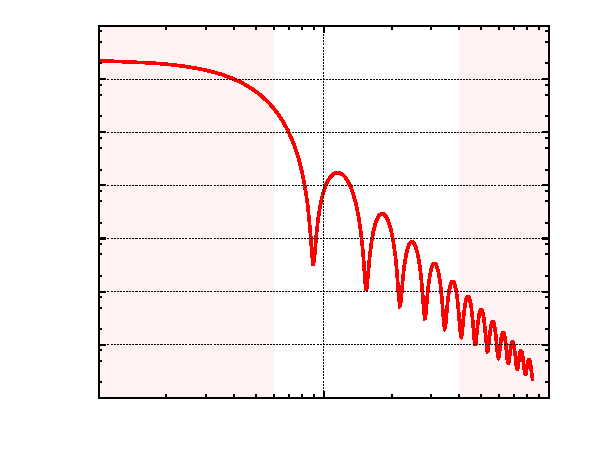
\includegraphics{ScatteringCurve50nm}}%
    \gplfronttext
  \end{picture}%
\endgroup
}\label{fig:ScatteringCurve50nm}}
\caption[The scattering curve and its relevant regions.]{a) Radially symmetric scattering pattern of a nanoparticle ensemble in suspension with radius 50 nm and a polydispersity degree of 25 $\%$. b) The scattering curve is the azimuthal integration of the 2D image. The three different regions of the scattering curve discussed in the text are highlighted in the figure as well.}
\end{figure*}

For isotropically scattering samples, the scattering patterns consist of concentric rings, as shown in figure \ref{fig:Au100ScatteringPattern}. By azimuthally averaging the scattering pattern, the data is reduced from 2D images to 1D scattering curves. The scattering curve is the typical form to present the experimental data, which displays the differential scattering cross-section per volume $\sfrac{d\Sigma}{d\Omega}$ versus the momentum transfer $q$ in a log–log graph as depicted in figure \ref{fig:ScatteringCurve50nm} for an ensemble of spherical particles with radius 50 nm and polydispersity degree 25 $\%$. Three different regions can be distinguished in a scattering curve \citep{schnablegger_practical_2006}:

\begin{itemize}
        \item The \textbf{Guinier region} comprises the low-$q$ region where $qD<1.3$ \citep{feigin_structure_1987}, being $D$ the characteristic length of the investigated object. This region provides principally information about the size of the particle.
        \item The high-$q$ region is called the \textbf{Porod region}, where information about the surface-to-volume ratio of the particles can be derived. For a smooth particle surface, the scattering intensity decays as $q^{-4}$, while for rough or fractal surfaces the slope is a function of $q^{-b}$ with $2<b<4$ \citep{glatter_small_1982}.
        \item For sufficiently monodisperse particle suspensions, the \textbf{Fourier region} or middle-$q$ region of the scattering curve shows pronounced minima that characterize the particle structure, size and shape.

\end{itemize}

\subsection{Modelling of the scattering intensity: Form factors}

Besides the information obtained about the size distribution of the particle ensemble, the scattering intensity $I(q)$ provides information about the shape and composition of the particles, accessible by modelling the form factor. In the simple case of a solid sphere with uniform density $\rho_0$, the radial electron density profile is described by $\rho_e(r>R)=0$ and $\rho_e(r<R)=\rho_0$, whilst the integral of expression \ref{eq:FormFactorSpherical} is limited only to the radius of the particle $R$. The form factor of a homogeneous solid sphere is 

\begin{equation}
        \label{eq:ff_sphere}
       f_{\text{sph}}(q,R)=\frac{4}{3}\pi R^3 \left( \rho_0 - \rho_{\text{medium}} \right) \left( 3\frac{\sin(qR)-qR\cos(qR)}{\left( qR \right)^3} \right) = \Delta \eta \cdot F_{\text{sph}}(q,R)
\end{equation}

where $\Delta \eta = \rho_0 - \rho_{\text{medium}}$ is the contrast and $ F_{\text{sph}}(q,R)$ is defined for convenience. When the shape of the particle deviates from a sphere, the assumptions made in equation \ref{eq:FormFactorSpherical} are not applicable and the scattering intensity must be integrated over all available angles numerically. For a homogeneous ellipsoid of revolution with two equal semi-axes of length $R$ and a semi-principal axis of length $\nu R $, the square of the form factor is expressed as:

\begin{equation}
        \label{eq:ff_ellipsoid}
       \abs{ f_{\text{ellip}}(q,R) }^2 = \Delta \eta^2 \int_0^1 \abs{F_{\text{sph}}\left( q,R \sqrt{u^2\left( \nu^2 -1 \right) + 1} \right)}^2 du
\end{equation}

where $\nu$ is the ellipticity, $u = \cos{\alpha}$ and $\alpha \in \left[  0, \sfrac{\pi}{2} \right]$. If $\nu > 1$, the expression defines a prolate spheroid, whilst $\nu < 1$ defines an oblate spheroid.

Frequently, nanoparticles show an internal heterogeneity, leading to an inner electron density distribution. If the components are radially distinguishable, the form factor corresponding to a morphology defined by sharp interfaces between the radial symmetric components of the particle with radius \(R_i\) is

\begin{equation}
\label{eq:multicore-shell}
f\left(q,R \right)= \Delta \eta F_{\text{sph}}(q,R)+\sum_{i=1}^{n-1} \Delta\rho_i \left( F_{\text{sph}}(q,R_{i+1})-F_{\text{sph}}(q,R_{i}) \right) ,
\end{equation}

where \(R\) is the external radius of the particle and \( n \) is the number of concentric shells. The excess of electron density of each component is $\Delta\rho_i = \rho_i - \rho_{\text{core}}$ and the contrast is defined in this case as $\Delta \eta = \rho_{\text{core}} - \rho_{\text{medium}}$ in order to isolate the electron density of the surrounding medium in one term.

The simplest case of expression \ref{eq:multicore-shell} arises for core-shell particles in suspension. This model represents a radially symmetric particle with a sharp interface between the outer shell and the inner core. The form factor is described by

\begin{equation}
        \label{eq:ff_cs}
	f_{\text{CS}}(q,R)=  \Delta\eta F_{\text{sph}}(q,R) +  \Delta\rho\left( F_{\text{sph}}(q,R)-F_{\text{sph}}(q,R_{\text{core}}) \right) ,
\end{equation}

where \(R \) and \(R_{\text{core}} \)  are the outer shell and inner core radii respectively, the excess of electron density is \(\Delta\rho=\rho_{\text{shell}}-\rho_{\text{core}}\) and the contrast is expressed as \(\Delta\eta=\rho_{\text{core}}-\rho_{\text{solv}}\), where $\rho_{\text{solv}}$ is the electron density of the suspending medium.

Depending on the synthesis of the particles, the interface between the different phases might show a linear electron density gradient between the particle's components. Analogously to expression \ref{eq:multicore-shell}, the form factor of a multicomponent spherical particle with a linear gradient interface is

\begin{equation}
f\left(q,R \right) = \sum_{i=0}^{n-1}\left[m_i \left( F_{\text{lin}}(q,R_{i+1})-F_{\text{lin}}(q,R_{i}) \right) +b_i \left( F_{\text{sph}}(q,R_{i+1})-F_{\text{sph}}(q,R_{i}) \right) \right]
\end{equation}
where $m_i=\sfrac{\left( \rho_{i+1}-\rho_{i} \right)}{\left( R_{i+1}-R_{i} \right)}$ and $b_i=\left( \rho_i-\rho_{\text{solv}} \right)-R_im_i$ and the linear form factor is defined by
\begin{equation}
F_{\text{lin}}(q,R) = 4\pi\frac{ \left( 2qR\sin(qR)+2\cos(qR)-(qR)^2\cos(qR) \right)}{q^4}
\end{equation}

The presented form factors are the models used in this work to analyse the experimental SAXS data of nanoparticles in suspension which will be discussed in chapters \ref{chap:density_gradient_SAXS}, \ref{chap:simultaneous_size_density} and \ref{chap:bio_applications}.

\section{Contrast variation}
\label{sec:contrast_variation_theory}

In the contrast variation method, the electron density of the particle or the surrounding medium is systematically altered in order to obtain independent scattering curves with different contrasts $\Delta \eta (r)$. This technique is useful to characterize the different components of heterogeneous particles, due to the complementary data that can be collected at each contrast. The work presented in this thesis is focused in the \emph{solvent contrast variation} method, where only the electron density of the suspending medium is varied.

\begin{figure*}%[htbp]
	\centering
		\subfloat[Core-shell particle in solvent]{\resizebox{0.44\linewidth}{!}{\fontsize{25pt}{25pt}\selectfont\input{Figures/ContrastScheme.pdf_tex}}\label{fig:ContrastScheme}}
		\qquad
		\subfloat[Contrast matching of the shell]{\resizebox{0.44\linewidth}{!}{\fontsize{25pt}{25pt}\selectfont\input{Figures/MatchPointScheme.pdf_tex}}\label{fig:MatchPointScheme}}
	\caption[Solvent contrast variation experiment and contrast matching scheme.]{Variation of the solvent electron density represented by the electron density profile of a spherical core-shell particle: a) The contrast of both core and shell components is high ($\Delta\eta_{\text{core}} > \Delta\eta_{\text{shell}} > 0$), while in figure b) the solvent electron density is increased to match the shell's ($\Delta\eta_{\text{shell}} = 0$). In this case, the only contribution to the scattering intensity will arise from the core.}
\end{figure*}


By means of the solvent contrast variation approach, the electron density of a single phase of the investigated particle can be matched (i.e. \emph{match point}), resulting in a increased scattering amplitude of the other components of the object, as depicted in figures \ref{fig:ContrastScheme} and \ref{fig:MatchPointScheme}. This effect enables a much more detailed study of the different contributions of the particle's components to the scattering intensity, which can be isolated by choosing the solvent electron density appropriately. In the following paragraphs, the theoretical framework required to interpret a SAXS contrast variation experiment will be presented, focusing mainly on the effects produced by the variation of the solvent electron density $\rho_{\text{solv}}$.

 
\subsection{Isoscattering point}
\label{sec:isopoint_theory}
One of the best known features appearing in a contrast variation experiment with heterogeneous nanoparticles is the existence of \emph{isoscattering points}, first formulated by \cite{kawaguchi_x-ray_1983-1}. At these specific \( q\)-values, the scattering intensity is independent of the adjusted solvent contrast, i.e. all scattering curves intersect in the isoscattering points regardless of the contrast. The isoscattering points \(q^{\star}\) are particularly interesting because they emerge for any spherical particle with an inner structure and a sufficiently narrow size distribution. From the contrast-depending part of equation \eqref{eq:multicore-shell}, a model-free expression can be derived which relates the position of the isoscattering points \(q^{\star}_i\) with the external radius of the particle \( R \), independent of its radial structure \citep{kawaguchi_x-ray_1983-1,kawaguchi_isoscattering_1992}:

\begin{equation}
        \label{eq:isoscattering}
        \tan(q^{\star}_iR)=q^{\star}_iR
\end{equation}

The solutions for this equation fulfill $q^{\star} R =4.493, 7.725, 10.904, ...$, where the positions of the isoscattering points correspond to the minima positions of the scattering intensity of a compact spherical particle with radius \( R \). This expression relates in a simple way the position of $q^{\star}$ to the size of the particle inaccessible to the suspending medium and, thus, a good method to determine the diameter of the colloid.

Although this expression is derived for the monodisperse case, it can still be applied up to a moderate degree of polydispersity, if care is taken regarding the shift of the minima position due to polydispersity \citep{beurten_polydispersity_1981}. For size distributions with \( p_d\) larger than \( \approx 30\,\% \), the isoscattering point is not well defined and the intersection point of the curves is smeared out, showing a diffuseness in the isoscattering point position \citep{kawaguchi_isoscattering_1992}. The effect of polydispersity in the isoscattering point is illustrated by simulating a 100 nm core-shell particle for the ideal case of a monodisperse ensemble (figure \ref{fig:IsopointSimulationIdeal}) and with a degree of polydispersity of 30 $\%$ (figure \ref{fig:IsopointSimulationPolydisperse}). The shift of the isoscatterig point position to smaller $q$-values and the diffuseness of the intersection point due to the high $p_d$ are clearly evident in the inset of figure \ref{fig:IsopointSimulationPolydisperse}.

Similarly, any deviation from the spherical shape produces a diffuseness in the $q^{\star}$ position. Unfortunately, this effect cannot be distinguished from the smearing produced by the size polydispersity and the investigation of the particle shape needs to be performed by other means.

\begin{figure*}%[htbp]
	\centering
		\subfloat[Monodisperse nanoparticles]{\resizebox{0.45\linewidth}{!}{\figfont{12pt}% GNUPLOT: LaTeX picture with Postscript
\begingroup
  \makeatletter
  \providecommand\color[2][]{%
    \GenericError{(gnuplot) \space\space\space\@spaces}{%
      Package color not loaded in conjunction with
      terminal option `colourtext'%
    }{See the gnuplot documentation for explanation.%
    }{Either use 'blacktext' in gnuplot or load the package
      color.sty in LaTeX.}%
    \renewcommand\color[2][]{}%
  }%
  \providecommand\includegraphics[2][]{%
    \GenericError{(gnuplot) \space\space\space\@spaces}{%
      Package graphicx or graphics not loaded%
    }{See the gnuplot documentation for explanation.%
    }{The gnuplot epslatex terminal needs graphicx.sty or graphics.sty.}%
    \renewcommand\includegraphics[2][]{}%
  }%
  \providecommand\rotatebox[2]{#2}%
  \@ifundefined{ifGPcolor}{%
    \newif\ifGPcolor
    \GPcolortrue
  }{}%
  \@ifundefined{ifGPblacktext}{%
    \newif\ifGPblacktext
    \GPblacktextfalse
  }{}%
  % define a \g@addto@macro without @ in the name:
  \let\gplgaddtomacro\g@addto@macro
  % define empty templates for all commands taking text:
  \gdef\gplbacktext{}%
  \gdef\gplfronttext{}%
  \makeatother
  \ifGPblacktext
    % no textcolor at all
    \def\colorrgb#1{}%
    \def\colorgray#1{}%
  \else
    % gray or color?
    \ifGPcolor
      \def\colorrgb#1{\color[rgb]{#1}}%
      \def\colorgray#1{\color[gray]{#1}}%
      \expandafter\def\csname LTw\endcsname{\color{white}}%
      \expandafter\def\csname LTb\endcsname{\color{black}}%
      \expandafter\def\csname LTa\endcsname{\color{black}}%
      \expandafter\def\csname LT0\endcsname{\color[rgb]{1,0,0}}%
      \expandafter\def\csname LT1\endcsname{\color[rgb]{0,1,0}}%
      \expandafter\def\csname LT2\endcsname{\color[rgb]{0,0,1}}%
      \expandafter\def\csname LT3\endcsname{\color[rgb]{1,0,1}}%
      \expandafter\def\csname LT4\endcsname{\color[rgb]{0,1,1}}%
      \expandafter\def\csname LT5\endcsname{\color[rgb]{1,1,0}}%
      \expandafter\def\csname LT6\endcsname{\color[rgb]{0,0,0}}%
      \expandafter\def\csname LT7\endcsname{\color[rgb]{1,0.3,0}}%
      \expandafter\def\csname LT8\endcsname{\color[rgb]{0.5,0.5,0.5}}%
    \else
      % gray
      \def\colorrgb#1{\color{black}}%
      \def\colorgray#1{\color[gray]{#1}}%
      \expandafter\def\csname LTw\endcsname{\color{white}}%
      \expandafter\def\csname LTb\endcsname{\color{black}}%
      \expandafter\def\csname LTa\endcsname{\color{black}}%
      \expandafter\def\csname LT0\endcsname{\color{black}}%
      \expandafter\def\csname LT1\endcsname{\color{black}}%
      \expandafter\def\csname LT2\endcsname{\color{black}}%
      \expandafter\def\csname LT3\endcsname{\color{black}}%
      \expandafter\def\csname LT4\endcsname{\color{black}}%
      \expandafter\def\csname LT5\endcsname{\color{black}}%
      \expandafter\def\csname LT6\endcsname{\color{black}}%
      \expandafter\def\csname LT7\endcsname{\color{black}}%
      \expandafter\def\csname LT8\endcsname{\color{black}}%
    \fi
  \fi
  \setlength{\unitlength}{0.0500bp}%
  \begin{picture}(5668.00,4534.00)%
    \gplgaddtomacro\gplbacktext{%
      \csname LTb\endcsname%
      \put(748,851){\makebox(0,0)[r]{\strut{}$10^{1}$}}%
      \csname LTb\endcsname%
      \put(748,1339){\makebox(0,0)[r]{\strut{}$10^{2}$}}%
      \csname LTb\endcsname%
      \put(748,1828){\makebox(0,0)[r]{\strut{}$10^{3}$}}%
      \csname LTb\endcsname%
      \put(748,2316){\makebox(0,0)[r]{\strut{}$10^{4}$}}%
      \csname LTb\endcsname%
      \put(748,2804){\makebox(0,0)[r]{\strut{}$10^{5}$}}%
      \csname LTb\endcsname%
      \put(748,3292){\makebox(0,0)[r]{\strut{}$10^{6}$}}%
      \csname LTb\endcsname%
      \put(748,3781){\makebox(0,0)[r]{\strut{}$10^{7}$}}%
      \csname LTb\endcsname%
      \put(748,4269){\makebox(0,0)[r]{\strut{}$10^{8}$}}%
      \csname LTb\endcsname%
      \put(1365,484){\makebox(0,0){\strut{} 0.02}}%
      \csname LTb\endcsname%
      \put(2235,484){\makebox(0,0){\strut{} 0.05}}%
      \csname LTb\endcsname%
      \put(2894,484){\makebox(0,0){\strut{} 0.1}}%
      \csname LTb\endcsname%
      \put(3552,484){\makebox(0,0){\strut{} 0.2}}%
      \csname LTb\endcsname%
      \put(4422,484){\makebox(0,0){\strut{} 0.5}}%
      \put(176,2486){\rotatebox{-270}{\makebox(0,0){\strut{}Scattering Intensity / a.u.}}}%
      \put(2651,154){\makebox(0,0){\strut{}$q$ / nm$^{-1}$}}%
    }%
    \gplgaddtomacro\gplfronttext{%
      \csname LTb\endcsname%
      \put(4853,704){\makebox(0,0)[l]{\strut{}\smaller -100}}%
      \put(4853,1149){\makebox(0,0)[l]{\strut{}\smaller -80}}%
      \put(4853,1595){\makebox(0,0)[l]{\strut{}\smaller -60}}%
      \put(4853,2040){\makebox(0,0)[l]{\strut{}\smaller -40}}%
      \put(4853,2486){\makebox(0,0)[l]{\strut{}\smaller -20}}%
      \put(4853,2932){\makebox(0,0)[l]{\strut{}\smaller 0}}%
      \put(4853,3377){\makebox(0,0)[l]{\strut{}\smaller 20}}%
      \put(4853,3823){\makebox(0,0)[l]{\strut{}\smaller 40}}%
      \put(4853,4269){\makebox(0,0)[l]{\strut{}\smaller 60}}%
      \put(5283,2486){\rotatebox{-90}{\makebox(0,0){\strut{}\smaller $\Delta \eta$ / nm$^{-3}$}}}%
    }%
    \gplgaddtomacro\gplbacktext{%
      \csname LTb\endcsname%
      \put(3334,3131){\makebox(0,0){\strut{}\smaller 0.08}}%
      \csname LTb\endcsname%
      \put(3817,3131){\makebox(0,0){\strut{}\smaller 0.09}}%
      \csname LTb\endcsname%
      \put(4250,3131){\makebox(0,0){\strut{}\smaller 0.1}}%
    }%
    \gplgaddtomacro\gplfronttext{%
    }%
    \gplbacktext
    \put(0,0){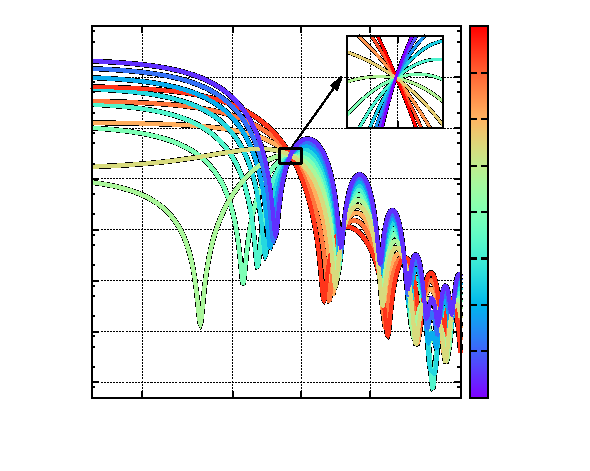
\includegraphics{IsopointSimulationIdeal}}%
    \gplfronttext
  \end{picture}%
\endgroup
}\label{fig:IsopointSimulationIdeal}}
		\qquad
		\subfloat[Polydisperse ensemble: $p_d=30\;\%$]{\resizebox{0.45\linewidth}{!}{\figfont{12pt}% GNUPLOT: LaTeX picture with Postscript
\begingroup
  \makeatletter
  \providecommand\color[2][]{%
    \GenericError{(gnuplot) \space\space\space\@spaces}{%
      Package color not loaded in conjunction with
      terminal option `colourtext'%
    }{See the gnuplot documentation for explanation.%
    }{Either use 'blacktext' in gnuplot or load the package
      color.sty in LaTeX.}%
    \renewcommand\color[2][]{}%
  }%
  \providecommand\includegraphics[2][]{%
    \GenericError{(gnuplot) \space\space\space\@spaces}{%
      Package graphicx or graphics not loaded%
    }{See the gnuplot documentation for explanation.%
    }{The gnuplot epslatex terminal needs graphicx.sty or graphics.sty.}%
    \renewcommand\includegraphics[2][]{}%
  }%
  \providecommand\rotatebox[2]{#2}%
  \@ifundefined{ifGPcolor}{%
    \newif\ifGPcolor
    \GPcolortrue
  }{}%
  \@ifundefined{ifGPblacktext}{%
    \newif\ifGPblacktext
    \GPblacktextfalse
  }{}%
  % define a \g@addto@macro without @ in the name:
  \let\gplgaddtomacro\g@addto@macro
  % define empty templates for all commands taking text:
  \gdef\gplbacktext{}%
  \gdef\gplfronttext{}%
  \makeatother
  \ifGPblacktext
    % no textcolor at all
    \def\colorrgb#1{}%
    \def\colorgray#1{}%
  \else
    % gray or color?
    \ifGPcolor
      \def\colorrgb#1{\color[rgb]{#1}}%
      \def\colorgray#1{\color[gray]{#1}}%
      \expandafter\def\csname LTw\endcsname{\color{white}}%
      \expandafter\def\csname LTb\endcsname{\color{black}}%
      \expandafter\def\csname LTa\endcsname{\color{black}}%
      \expandafter\def\csname LT0\endcsname{\color[rgb]{1,0,0}}%
      \expandafter\def\csname LT1\endcsname{\color[rgb]{0,1,0}}%
      \expandafter\def\csname LT2\endcsname{\color[rgb]{0,0,1}}%
      \expandafter\def\csname LT3\endcsname{\color[rgb]{1,0,1}}%
      \expandafter\def\csname LT4\endcsname{\color[rgb]{0,1,1}}%
      \expandafter\def\csname LT5\endcsname{\color[rgb]{1,1,0}}%
      \expandafter\def\csname LT6\endcsname{\color[rgb]{0,0,0}}%
      \expandafter\def\csname LT7\endcsname{\color[rgb]{1,0.3,0}}%
      \expandafter\def\csname LT8\endcsname{\color[rgb]{0.5,0.5,0.5}}%
    \else
      % gray
      \def\colorrgb#1{\color{black}}%
      \def\colorgray#1{\color[gray]{#1}}%
      \expandafter\def\csname LTw\endcsname{\color{white}}%
      \expandafter\def\csname LTb\endcsname{\color{black}}%
      \expandafter\def\csname LTa\endcsname{\color{black}}%
      \expandafter\def\csname LT0\endcsname{\color{black}}%
      \expandafter\def\csname LT1\endcsname{\color{black}}%
      \expandafter\def\csname LT2\endcsname{\color{black}}%
      \expandafter\def\csname LT3\endcsname{\color{black}}%
      \expandafter\def\csname LT4\endcsname{\color{black}}%
      \expandafter\def\csname LT5\endcsname{\color{black}}%
      \expandafter\def\csname LT6\endcsname{\color{black}}%
      \expandafter\def\csname LT7\endcsname{\color{black}}%
      \expandafter\def\csname LT8\endcsname{\color{black}}%
    \fi
  \fi
  \setlength{\unitlength}{0.0500bp}%
  \begin{picture}(5668.00,4534.00)%
    \gplgaddtomacro\gplbacktext{%
      \csname LTb\endcsname%
      \put(748,704){\makebox(0,0)[r]{\strut{}$10^{2}$}}%
      \csname LTb\endcsname%
      \put(748,1355){\makebox(0,0)[r]{\strut{}$10^{3}$}}%
      \csname LTb\endcsname%
      \put(748,2006){\makebox(0,0)[r]{\strut{}$10^{4}$}}%
      \csname LTb\endcsname%
      \put(748,2657){\makebox(0,0)[r]{\strut{}$10^{5}$}}%
      \csname LTb\endcsname%
      \put(748,3308){\makebox(0,0)[r]{\strut{}$10^{6}$}}%
      \csname LTb\endcsname%
      \put(748,3958){\makebox(0,0)[r]{\strut{}$10^{7}$}}%
      \csname LTb\endcsname%
      \put(1365,484){\makebox(0,0){\strut{} 0.02}}%
      \csname LTb\endcsname%
      \put(2235,484){\makebox(0,0){\strut{} 0.05}}%
      \csname LTb\endcsname%
      \put(2894,484){\makebox(0,0){\strut{} 0.1}}%
      \csname LTb\endcsname%
      \put(3552,484){\makebox(0,0){\strut{} 0.2}}%
      \csname LTb\endcsname%
      \put(4422,484){\makebox(0,0){\strut{} 0.5}}%
      \put(176,2486){\rotatebox{-270}{\makebox(0,0){\strut{}Scattering Intensity / a.u.}}}%
      \put(2651,154){\makebox(0,0){\strut{}$q$ / nm$^{-1}$}}%
    }%
    \gplgaddtomacro\gplfronttext{%
      \csname LTb\endcsname%
      \put(4853,704){\makebox(0,0)[l]{\strut{}\smaller -100}}%
      \put(4853,1149){\makebox(0,0)[l]{\strut{}\smaller -80}}%
      \put(4853,1595){\makebox(0,0)[l]{\strut{}\smaller -60}}%
      \put(4853,2040){\makebox(0,0)[l]{\strut{}\smaller -40}}%
      \put(4853,2486){\makebox(0,0)[l]{\strut{}\smaller -20}}%
      \put(4853,2932){\makebox(0,0)[l]{\strut{}\smaller 0}}%
      \put(4853,3377){\makebox(0,0)[l]{\strut{}\smaller 20}}%
      \put(4853,3823){\makebox(0,0)[l]{\strut{}\smaller 40}}%
      \put(4853,4269){\makebox(0,0)[l]{\strut{}\smaller 60}}%
      \put(5283,2486){\rotatebox{-90}{\makebox(0,0){\strut{}\smaller $\Delta \eta$ / nm$^{-3}$}}}%
    }%
    \gplgaddtomacro\gplbacktext{%
      \csname LTb\endcsname%
      \put(3609,3131){\makebox(0,0){\strut{}\smaller 0.08}}%
      \csname LTb\endcsname%
      \put(4110,3131){\makebox(0,0){\strut{}\smaller 0.09}}%
    }%
    \gplgaddtomacro\gplfronttext{%
    }%
    \gplbacktext
    \put(0,0){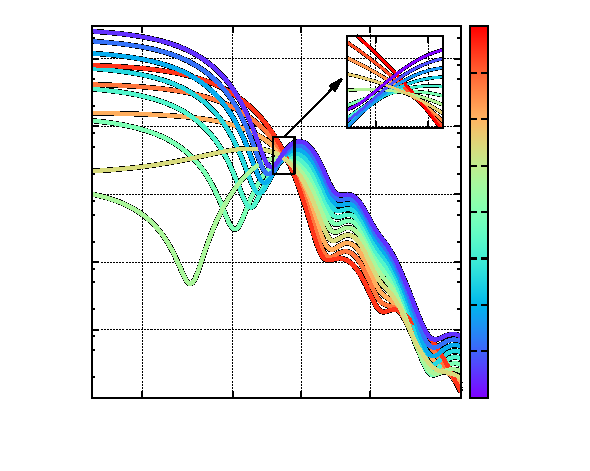
\includegraphics{IsopointSimulationPolydisperse}}%
    \gplfronttext
  \end{picture}%
\endgroup
}\label{fig:IsopointSimulationPolydisperse}}
	\caption[Isoscattering points and particle polydispersity.]{A isoscattering point is the $q$-value where all the scattering curves measured at different contrasts $\Delta \eta$ intersect. a) In the monodisperse case, the first isoscattering point is well-defined as depicted in the inset, while the inset of b) shows how the high polydispersity of the ensemble produces a diffuse isoscattering point and the intersection point is smeared out.}
\end{figure*}

\subsection{Basic functions approach}
\label{sec:basic_functions_theory}
When analysing contrast variation data, a widespread theoretical approach is based on the non-interacting model proposed by Stuhrmann $\&$ Kirste (\citeyear{stuhrmann_elimination_1965,stuhrmann_elimination_1967}) for monodisperse particles. The so-called \emph{basic functions} formulation differentiates, independently of the particle inner structure, the contributions which depend on the varying solvent density or contrast (\(\Delta\eta\)) and on the excess of electron density of each component of the particle.

Deriving from this approach, the scattering intensity can be expressed as the combination of contributions corresponding to different features of the particles:
\begin{equation}
\label{eq:intensity_contrast}
I(q)=I_c(q)+\Delta\eta I_{sc}(q)+(\Delta\eta)^2 I_{s}(q)
\end{equation}
The $I_c$ function contains the contributions from the density fluctuations inside the particle, the contribution $I_s$ is the so-called \emph{shape scattering function} and $I_{sc}$ is the cross-term function.

\subsubsection{Shape scattering function}
The $I_s(q)$ function corresponds to the scattering contributions from particles with homogeneous density and a size equivalent to the volume inaccessible to the solvent, typically the external size of the nanoparticle. By modelling the shape scattering function, the shape and size distribution of the particles can be determined independently of their inner structure. The functions $I_{sc}(q)$ and $I_{c}(q)$ are more rarely employed due to their complex interpretation. $I_{c}(q)$ contains the electron density deviations in the particle from the average electron density, while $I_{sc}(q)$ includes crossed contributions from both $I_{c}(q)$ and $I_{s}(q)$.

In a system measured at $N$ different solvent electron densities i.e. contrasts, the shape scattering function $I_s$ at each $q$-value can be calculated by solving the following matrix equation:

\begin{equation}
  \begin{pmatrix}
  I_1(q) \\
  \vdots \\
  I_N(q) \\
 \end{pmatrix}
  = 
 \begin{pmatrix}
  1 & \Delta \eta_1 &  \left( \Delta \eta_1 \right)^2 \\
  \vdots  & \vdots  & \vdots  \\
  1 & \Delta \eta_N &  \left( \Delta \eta_N \right)^2 
 \end{pmatrix}
 \begin{pmatrix}
  I_c(q) \\
  I_{sc}(q) \\
  I_s(q) \\
 \end{pmatrix}
\end{equation}

where $I_i (q)$ is the measured scattering intensity at each solvent electron density and $\Delta \eta _i$ is the contrast corresponding to each suspending medium density. A minimum of 3 independent scattering curves measured at different contrasts are required to solve this system of equations, while an accurate determination of the suspending medium electron density is also necessary for the calculation of the different $\Delta \eta _i$.

\subsubsection{Guinier approximation}
\label{sec:TheoryGuinier}

The radius of gyration of a particle about its centre of mass $R_g$ is defined as the second moment of the electron density distribution and can be calculated by 

\begin{equation}
        R_g^2 = \frac{\int \rho_e (r) r^2 dr}{\int \rho_e (r)  dr}
\end{equation}

The radius of gyration is systematically employed in small-angle scattering as an evaluation tool, due to its applicability to a large diversity of samples, e.g. proteins, colloids, suprastructures \citep{mertens_structural_2010,sim_salt_2012}. If the object is spherical, the gyration radius is directly related with its external radius by $R_g^2 = \sfrac{3}{5}R^2$.

In SAXS, $R_g$ can be calculated using the Guinier approximation \citep{guinier_diffraction_1939,guinier_small-angle_1955}, which assumes that the scattering intensity behaves in the limit of small \(q\) as

\begin{equation}
\label{eq:guinier}
I(q) \simeq I(0)\,\mbox{exp}\left(-\frac{R_g^2}{3}q^2\right),
\end{equation}

where \( I(0)\) is known as forward scattering or intensity at zero angle. Using the basic functions approach, the radius of gyration of a monodisperse, heterogeneous particle can be expressed as a function of the solvent electron density \( \rho_{\text{solv}} \) and the average electron density of the particle \( \rho_0 \) \citep{feigin_structure_1987}
\begin{equation}
R_g^2=R_{g,c}^{\,2}+\frac{\alpha}{\rho_0-\rho_{\text{solv}}}-\frac{\beta}{(\rho_0-\rho_{\text{solv}})^2},
\label{eq:gyration}
\end{equation}
where \(R_{g,c}\) is the radius of gyration of the particle shape corresponding to the volume inaccessible for the solvent \( V_c \), \( \alpha \) characterizes the distribution of different phases inside the particle and \( \beta>0 \) considers the eccentricity of the different scattering contributions \citep{stuhrmann_small-angle_2008}. Particle aggregation influences the scattering curves especially in the Guinier region and must be explicitly avoided.

\cite{avdeev_contrast_2007} proposed an extended version to equation \eqref{eq:gyration} for the case of a polydisperse particle ensemble by introducing the \emph{effective} values \( \tilde R^2_{g,c} \), \( \tilde \alpha \) and \( \tilde \beta \), which are the intensity-weighted averages of the corresponding parameters over the polydispersity. The observed average electron density is not affected by the polydispersity (\( \tilde\rho_0=\rho_0 \)) if the volume ratio between the different particle components is constant for all particles in the ensemble.

Assuming the premise of a constant average electron density for all the particles, the intensity at zero angle for a polydisperse system can be expressed as

\begin{equation}
\label{eq:I0}
I(0)\propto N \left( \rho_0-\rho_{\text{solv}} \right)^2 ,
\end{equation}

with a minimum of the parabolic function at \( \rho_{\text{solv}}=\rho_0 \). Therefore, by analysing the Guinier region of the scattering curves in a contrast variation experiment, the average electron density of the particle can be obtained without assuming an \emph{a priori} inner structure.

Using the models presented above, it is possible to obtain by independent means the external radius and the average electron density of the particles in suspension.

	
	\chapter{Experimental setup for SAXS measurements}
\label{chap:experimental_setup}
\blindtext[1]\cite{ballauff_saxs_2001-1}
\section{BESSY II}

\section{FCM Beamline}
\subsection{Transmission measurements}
calibrated diodes, SYRES II????

\section{Small-angle X-ray scattering}
\subsection{Pilatus detector}
high dynamic range
noise free
\subsection{HZB SAXS setup}
\subsubsection{distance calibration}
10-4 uncertainty

\subsection{Radial integration and error propagation}
\subsection{Absolute intensity calibration}
\subsubsection{Flux monitor}
thin diode
\subsubsection{Detector efficiceny}
pilatus and thin diode

\section{Continuous contrast variation}
\subsection{Filling of capilaries}
galden at bottom, reference layer
\subsubsection{Capillary homogeneity}
Hilgenberg

\subsection{Calibration of solvent density and finding of main axis}
\subsection{Limitations}
\subsubsection{Density range}
sucrose, fructose, iodixanol
\subsubsection{Challenges with different contrast agents}
Background subtraction, induced aggregation by heavy salts
\subsubsection{Comparison to other contrast variation scattering techinques}
SANS (deuterated water)
RSoXS in polymeric colloids (H.Abe 2006), Carbon K-edge


	
	\chapter{Continuous contrast variation in SAXS: the density gradient technique}
\label{chap:density_gradient_SAXS}
\textcolor{red}{INTRODUCTION PARAGRAPH?????}

The contrast variation method in Small Angle X-ray Scattering (SAXS) experiments consists in systematically varying the electron density of the dispersing media to study the different contributions to the scattering intensity in greater detail as compared to measurements at a single contrast. It emerges as an ideally suited technique to elucidate the structure of particles with a complicated inner composition and has been repeatedly employed to investigate the radial structure of latex particles suspended in an aqueous medium \citet{dingenouts_analysis_1999,ballauff_analysis_2011}. In Small Angle Neutron Scattering (SANS) the contrast variation technique is widely used by mixing water and deuterium oxide, but the use of deuterated chemicals and the incoherent contribution to the background as well as the limited access to neutrons restrict the application of this technique. Other methods for structural investigation (e.g. transmission electron microscopy \citet{joensson_morphology_1991,silverstein_microstructure_1989}) require prior treatment of the sample and are not ensemble averaged. 

In SAXS, the solvent contrast variation technique is achieved by adding a suitable contrast agent to the suspending medium (e.g. sucrose) and recording the scattering data as a function of the adjusted solvent electron density \( \rho_{solv} \) \citet{ballauff_saxs_2001-1,bolze_application_2003}. In order to resolve small changes of the radial structure, the average electron density of the colloidal particles must be close to the dispersant's, i.e., the \emph{match point} should be approached, where the average contrast of the particle vanishes. In the case of polymeric lattices with electron densities ranging from 335 to \(390 \mbox{ nm}^{-3}\), an aqueous sucrose solution is very well suited as the suspension medium, due to the easy realization of concentrated solutions with electron densities of up to \(400 \mbox{ nm}^{-3}\). Previous studies on globular solutes \citet{kawaguchi_isoscattering_1992} and the influence of the sucrose on the size distribution of vesicles \citet{kiselev_sucrose_2001-1} show the feasibility of this technique, while further studies have investigated the effect of the penetration of the solvent into the particles \citet{kawaguchi_isoscattering_1993}.

The preparation of a number of different sucrose solutions has been a major inconvenience in solvent contrast variation experiments, due to the tedious, time-consuming process, possible inaccuracy in the sucrose concentration and the discrete range of available solvent electron densities. In this chapter, a novel approach using a density gradient column is introduced, which allows the tuning of the solvent contrast within the provided density range, resulting in a virtually continuous solvent contrast variation. By filling the bottom part of the capillary with a particle dispersion in a concentrated sucrose solution and the top part with an aqueous solution of the same particle concentration, a solvent density gradient is initiated with a constant concentration of nanoparticles along the capillary. Density gradient columns are extensively used in fields like marine biology \citet{coombs_density-gradient_1981} or biochemistry together with centrifugation \citet{hinton_density_1978}, to create a continuously graded aqueous sucrose solution by diffusion of the sucrose molecules. By measuring the density gradient column at different points in time during the diffusion process of the sucrose, it is possible to choose \emph{in situ} the most appropriate solvent densities to perform measurements close to the contrast match point. Combining this approach with SAXS, a very extensive dataset with a virtually continuous variation in the suspending medium density can be acquired in a short interval of time.

The experimental details of the proposed approach are shown in section \ref{sec:DensityGradientExperimental}, followed by the example of the continuous contrast variation technique applied to a polymeric nanoparticle in section \ref{sec:KiskerResults}. The evaluation of the SAXS data using different methods is reviewed in section \ref{sec:KiskerResultsEvaluation}, jointly with the discussion of the experimental measurements. Finally in section \ref{sec:KiskerResultsSummary} a consistency check of the obtained results is presented and the applicability of the solvent contrast variation technique in SAXS is discussed.


\section{Experimental proceeding}
\label{sec:DensityGradientExperimental}
Firstly, the preparation of a nanoparticle suspension density gradient within a glass capillary using an aqueous sucrose solution is described in section \ref{sec:GradientPreparation}. Then in section \ref{sec:SolventCalibration}, the calibration of the solvent electron density through X-ray transmittance measurements at different positions along the capillary vertical axis is explained, followed by a detailed overview in section \ref{sec:DensityGradientSAXS} of the collection of scattering patterns at the calibrated capillary positions with distinct contrasts.


\subsection{Preparation of the density gradient capillaries}
\label{sec:GradientPreparation}
The solvent density gradient is prepared in the rectangular glass capillaries presented in section \ref{sec:sample_environment}, which are extraordinary homogeneous and show very uniform sample thickness within 0.9 $\%$ and glass thickness within 0.4 $\%$. The bottom end of the capillary is closed by welding and the lower section, up to a height of ca. \(1\) cm, is filled with Galden\(\textregistered\)PFPE SV90 from Solvay Plastics (Brussels, \emph{Belgium}). This fluid has an exceptionally high density of $1.69\,\mathrm{g/cm^3}$, low viscosity and is immiscible with aqueous solutions. Consequently, a uniform interface with the particle suspension is formed at the bottom, which is employed as reference position for the X-ray transmittance measurements. 

The studied nanoparticles in suspension are mixed with a high sucrose concentration (Sigma-Aldrich, Missouri, \emph{USA}) and diluted in an aqueous solution, creating two mixtures with different solvent densities but equal particle concentrations. Directly above the Galden fluid, the denser of these two mixtures is filled into the capillary using a syringe up to a height of about 1 cm. The lighter aqueous dilution is then filled on top of the aqueous sucrose solution along ca. 1 cm. By the time the two components come into contact, the density gradient is initiated and the sucrose starts diffusing along the ca. 20 mm length of the filled capillary.

The calculated diffusion timescale of the solvent density gradient is ca. 10 minutes, considering that the diffusion coefficient of sucrose in water at 25$^{\circ}$C is \(D=5.2 \cdot 10^{-10} \;\frac{\mbox{m}^2}{\mbox{s}}\) \citep{uedaira_sugar-water_1985,ribeiro_binary_2006} and assuming that convection effects are negligible due to the small length-scale of the capillary \citep{berberan-santos_barometric_1997}. The time needed for the transfer of the sample into the UHV sample chamber amounts to ca. 1 hour. Within this time duration, the deviation of the solvent density at both ends of the gradient from the initial value can be estimated with an uncertainty below \(0.5\,\%\). 


\subsection{Calibration of the solvent density: X-ray transmission}
\label{sec:SolventCalibration}
The rectangular capillary is placed in the sample holder inside the UHV Reflectometer described in section \ref{sec:fcm} which allows the movement with micrometer precision in the directions perpendicular to the incoming beam, as depicted in figure \ref{fig:DensityGradientCapillarySetup}. In order to determine the central vertical capillary axis, a horizontal X-ray transmission scan is performed at two different vertical positions of the capillary spaced by 20 mm. The central vertical axis can be drawn from the centers of both measurements and the sample can be moved along this axis by the simultaneous operation of the vertical and horizontal motors.

\begin{figure}%[htbp]
	\centering
		\input{Figures/DensityGradientCapillarySetup.pdf_tex}
		\caption{The rectangular density gradient capillary is placed in the X-ray beam and can be moved by sample motors in both directions perpendicular to the incoming beam.}
		\label{fig:DensityGradientCapillarySetup}
\end{figure}

The transmitted intensity through the sample is recorded at a photon energy of \(E = (5500.0 \pm  0.5)\) eV for 10 seconds at each position. The measurement points are spaced 0.5 mm along the central vertical axis of the capillary, starting at the bottom reference interface with Galden\(\textregistered\)PFPE SV90. The overall X-ray transmission measurement requires approximately 5 minutes, which is within the calculated diffusion timescale of the aqueous sucrose solution. This transmission measurement is performed both immediately before and after recording the scattering patterns, which should not take much longer than the sucrose diffusion timescale (15-20 min). The transmittance values used for the density calibration are then linearly interpolated between both data sets taking into account the time-dependence. 

These values can be converted to solvent electron densities via the Beer-Lambert law introduced in section \ref{sec:BeerLambert}, which relates the density of the solution with the transmitted intensity:

\begin{equation}
  \rho(z) = A \left( \ln{I_0} - \ln{I(z)} \right) .
\end{equation}

Here \(\rho\) is the electron density of the suspending medium, $I$ and $I_0$ are the transmitted and incoming intensities respectively and $A$ is a factor determined by the reference values of the solvent electron density at the vertical limits of the capillary at the initial time. The sucrose concentration in solution expressed as the mass fraction \( M \) at these reference points can be converted to electron densities with the empirical formula \( \rho=1.2681M+333.19 \) nm\(^{-3}\) \citep{haynes_crc_2012}. The solvent electron density profile within the density gradient capillary derived from this measurement is depicted in figure \ref{fig:KiskerTransmissionCalibration} for 100 nm polystyrene particles at different diffusion times. The suspending medium electron density shows a maximum uncertainty of 1 nm$^{-3}$ at the interface between the two mixtures associated with the vertical size of the focused X-ray beam.

\begin{figure}%[htbp]
	\centering
		% GNUPLOT: LaTeX picture with Postscript
\begingroup
  \makeatletter
  \providecommand\color[2][]{%
    \GenericError{(gnuplot) \space\space\space\@spaces}{%
      Package color not loaded in conjunction with
      terminal option `colourtext'%
    }{See the gnuplot documentation for explanation.%
    }{Either use 'blacktext' in gnuplot or load the package
      color.sty in LaTeX.}%
    \renewcommand\color[2][]{}%
  }%
  \providecommand\includegraphics[2][]{%
    \GenericError{(gnuplot) \space\space\space\@spaces}{%
      Package graphicx or graphics not loaded%
    }{See the gnuplot documentation for explanation.%
    }{The gnuplot epslatex terminal needs graphicx.sty or graphics.sty.}%
    \renewcommand\includegraphics[2][]{}%
  }%
  \providecommand\rotatebox[2]{#2}%
  \@ifundefined{ifGPcolor}{%
    \newif\ifGPcolor
    \GPcolortrue
  }{}%
  \@ifundefined{ifGPblacktext}{%
    \newif\ifGPblacktext
    \GPblacktextfalse
  }{}%
  % define a \g@addto@macro without @ in the name:
  \let\gplgaddtomacro\g@addto@macro
  % define empty templates for all commands taking text:
  \gdef\gplbacktext{}%
  \gdef\gplfronttext{}%
  \makeatother
  \ifGPblacktext
    % no textcolor at all
    \def\colorrgb#1{}%
    \def\colorgray#1{}%
  \else
    % gray or color?
    \ifGPcolor
      \def\colorrgb#1{\color[rgb]{#1}}%
      \def\colorgray#1{\color[gray]{#1}}%
      \expandafter\def\csname LTw\endcsname{\color{white}}%
      \expandafter\def\csname LTb\endcsname{\color{black}}%
      \expandafter\def\csname LTa\endcsname{\color{black}}%
      \expandafter\def\csname LT0\endcsname{\color[rgb]{1,0,0}}%
      \expandafter\def\csname LT1\endcsname{\color[rgb]{0,1,0}}%
      \expandafter\def\csname LT2\endcsname{\color[rgb]{0,0,1}}%
      \expandafter\def\csname LT3\endcsname{\color[rgb]{1,0,1}}%
      \expandafter\def\csname LT4\endcsname{\color[rgb]{0,1,1}}%
      \expandafter\def\csname LT5\endcsname{\color[rgb]{1,1,0}}%
      \expandafter\def\csname LT6\endcsname{\color[rgb]{0,0,0}}%
      \expandafter\def\csname LT7\endcsname{\color[rgb]{1,0.3,0}}%
      \expandafter\def\csname LT8\endcsname{\color[rgb]{0.5,0.5,0.5}}%
    \else
      % gray
      \def\colorrgb#1{\color{black}}%
      \def\colorgray#1{\color[gray]{#1}}%
      \expandafter\def\csname LTw\endcsname{\color{white}}%
      \expandafter\def\csname LTb\endcsname{\color{black}}%
      \expandafter\def\csname LTa\endcsname{\color{black}}%
      \expandafter\def\csname LT0\endcsname{\color{black}}%
      \expandafter\def\csname LT1\endcsname{\color{black}}%
      \expandafter\def\csname LT2\endcsname{\color{black}}%
      \expandafter\def\csname LT3\endcsname{\color{black}}%
      \expandafter\def\csname LT4\endcsname{\color{black}}%
      \expandafter\def\csname LT5\endcsname{\color{black}}%
      \expandafter\def\csname LT6\endcsname{\color{black}}%
      \expandafter\def\csname LT7\endcsname{\color{black}}%
      \expandafter\def\csname LT8\endcsname{\color{black}}%
    \fi
  \fi
    \setlength{\unitlength}{0.0500bp}%
    \ifx\gptboxheight\undefined%
      \newlength{\gptboxheight}%
      \newlength{\gptboxwidth}%
      \newsavebox{\gptboxtext}%
    \fi%
    \setlength{\fboxrule}{0.5pt}%
    \setlength{\fboxsep}{1pt}%
\begin{picture}(8502.00,4534.00)%
    \gplgaddtomacro\gplbacktext{%
      \csname LTb\endcsname%
      \put(594,1050){\makebox(0,0)[r]{\strut{}$335$}}%
      \csname LTb\endcsname%
      \put(594,1614){\makebox(0,0)[r]{\strut{}$340$}}%
      \csname LTb\endcsname%
      \put(594,2178){\makebox(0,0)[r]{\strut{}$345$}}%
      \csname LTb\endcsname%
      \put(594,2742){\makebox(0,0)[r]{\strut{}$350$}}%
      \csname LTb\endcsname%
      \put(594,3306){\makebox(0,0)[r]{\strut{}$355$}}%
      \csname LTb\endcsname%
      \put(594,3870){\makebox(0,0)[r]{\strut{}$360$}}%
      \csname LTb\endcsname%
      \put(951,484){\makebox(0,0){\strut{}$0$}}%
      \csname LTb\endcsname%
      \put(1851,484){\makebox(0,0){\strut{}$2$}}%
      \csname LTb\endcsname%
      \put(2751,484){\makebox(0,0){\strut{}$4$}}%
      \csname LTb\endcsname%
      \put(3651,484){\makebox(0,0){\strut{}$6$}}%
      \csname LTb\endcsname%
      \put(4551,484){\makebox(0,0){\strut{}$8$}}%
      \csname LTb\endcsname%
      \put(5451,484){\makebox(0,0){\strut{}$10$}}%
      \put(6033,3996){\makebox(0,0)[l]{\strut{}$0.027$}}%
      \put(6033,3109){\makebox(0,0)[l]{\strut{}$0.028$}}%
      \put(6033,1835){\makebox(0,0)[l]{\strut{}$0.0295$}}%
      \put(6033,1022){\makebox(0,0)[l]{\strut{}$0.0305$}}%
    }%
    \gplgaddtomacro\gplfronttext{%
      \csname LTb\endcsname%
      \put(220,2486){\rotatebox{-270}{\makebox(0,0){\strut{}Solvent electron density / nm$^{-3}$}}}%
      \put(6736,2486){\rotatebox{270}{\makebox(0,0){\strut{}X-ray Transmission / $\%$}}}%
      \put(3313,154){\makebox(0,0){\strut{}Vertical Position / mm}}%
      \csname LTb\endcsname%
      \put(7476,704){\makebox(0,0)[l]{\strut{}\smaller 100}}%
      \put(7476,1213){\makebox(0,0)[l]{\strut{}\smaller 120}}%
      \put(7476,1722){\makebox(0,0)[l]{\strut{}\smaller 140}}%
      \put(7476,2231){\makebox(0,0)[l]{\strut{}\smaller 160}}%
      \put(7476,2741){\makebox(0,0)[l]{\strut{}\smaller 180}}%
      \put(7476,3250){\makebox(0,0)[l]{\strut{}\smaller 200}}%
      \put(7476,3759){\makebox(0,0)[l]{\strut{}\smaller 220}}%
      \put(7476,4269){\makebox(0,0)[l]{\strut{}\smaller 240}}%
      \put(7939,2486){\rotatebox{270}{\makebox(0,0){\strut{}\smaller Diffusion Time / min}}}%
    }%
    \gplbacktext
    \put(0,0){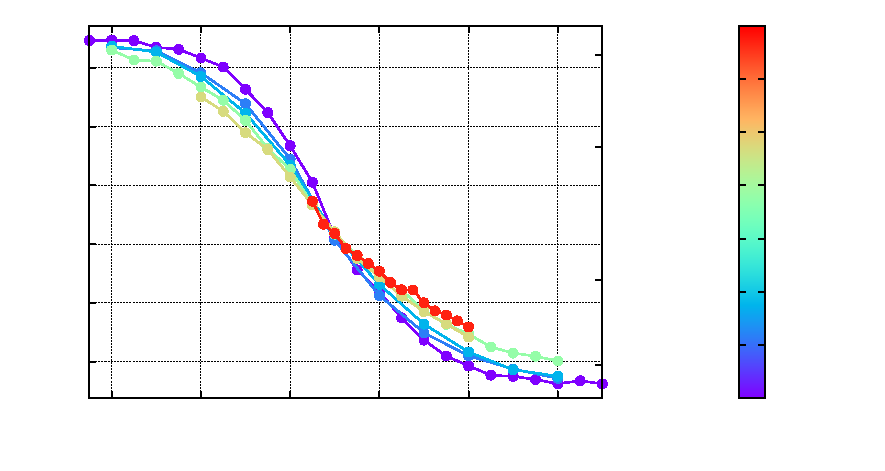
\includegraphics{KiskerTransmissionCalibration}}%
    \gplfronttext
  \end{picture}%
\endgroup

		\caption{Solvent density along the gradient capillary vertical axis, calculated from the transmission measurements at 5500 eV of 100 nm polystyrene particles. The corresponding X-ray transmission is also shown, revealing the low transmittances of the capillary at low energies.}
		\label{fig:KiskerTransmissionCalibration}
\end{figure}

The X-ray transmission measurements are performed at a low incident photon energy of $E = 5500$ eV to increase the transmittance differences for the less absorbing sucrose solution by, at least, a factor of 2.5. In figure \ref{fig:EnergiesTransmissionCalibration}, the calculated transmittances of a 65 $\%$ concentrated sucrose mixture and water (0 $\%$) are depicted, along with the ratio between both transmissions. This ratio decreases for high energies, suppressing the tranmission differences between both components of the density gradient column. This fact is revealed in figure \ref{fig:SucroseTransmissionCalibration}, where the X-ray transmittance of an aqueous sucrose density gradient measured at 5500 eV shows a better signal-to-noise ratio than the same measurement at 10000 eV.

\begin{figure}%[htbp]
	\centering
		\subfloat[Calculated transmittance]{\resizebox{0.44\linewidth}{!}{% GNUPLOT: LaTeX picture with Postscript
\begingroup
  \makeatletter
  \providecommand\color[2][]{%
    \GenericError{(gnuplot) \space\space\space\@spaces}{%
      Package color not loaded in conjunction with
      terminal option `colourtext'%
    }{See the gnuplot documentation for explanation.%
    }{Either use 'blacktext' in gnuplot or load the package
      color.sty in LaTeX.}%
    \renewcommand\color[2][]{}%
  }%
  \providecommand\includegraphics[2][]{%
    \GenericError{(gnuplot) \space\space\space\@spaces}{%
      Package graphicx or graphics not loaded%
    }{See the gnuplot documentation for explanation.%
    }{The gnuplot epslatex terminal needs graphicx.sty or graphics.sty.}%
    \renewcommand\includegraphics[2][]{}%
  }%
  \providecommand\rotatebox[2]{#2}%
  \@ifundefined{ifGPcolor}{%
    \newif\ifGPcolor
    \GPcolortrue
  }{}%
  \@ifundefined{ifGPblacktext}{%
    \newif\ifGPblacktext
    \GPblacktextfalse
  }{}%
  % define a \g@addto@macro without @ in the name:
  \let\gplgaddtomacro\g@addto@macro
  % define empty templates for all commands taking text:
  \gdef\gplbacktext{}%
  \gdef\gplfronttext{}%
  \makeatother
  \ifGPblacktext
    % no textcolor at all
    \def\colorrgb#1{}%
    \def\colorgray#1{}%
  \else
    % gray or color?
    \ifGPcolor
      \def\colorrgb#1{\color[rgb]{#1}}%
      \def\colorgray#1{\color[gray]{#1}}%
      \expandafter\def\csname LTw\endcsname{\color{white}}%
      \expandafter\def\csname LTb\endcsname{\color{black}}%
      \expandafter\def\csname LTa\endcsname{\color{black}}%
      \expandafter\def\csname LT0\endcsname{\color[rgb]{1,0,0}}%
      \expandafter\def\csname LT1\endcsname{\color[rgb]{0,1,0}}%
      \expandafter\def\csname LT2\endcsname{\color[rgb]{0,0,1}}%
      \expandafter\def\csname LT3\endcsname{\color[rgb]{1,0,1}}%
      \expandafter\def\csname LT4\endcsname{\color[rgb]{0,1,1}}%
      \expandafter\def\csname LT5\endcsname{\color[rgb]{1,1,0}}%
      \expandafter\def\csname LT6\endcsname{\color[rgb]{0,0,0}}%
      \expandafter\def\csname LT7\endcsname{\color[rgb]{1,0.3,0}}%
      \expandafter\def\csname LT8\endcsname{\color[rgb]{0.5,0.5,0.5}}%
    \else
      % gray
      \def\colorrgb#1{\color{black}}%
      \def\colorgray#1{\color[gray]{#1}}%
      \expandafter\def\csname LTw\endcsname{\color{white}}%
      \expandafter\def\csname LTb\endcsname{\color{black}}%
      \expandafter\def\csname LTa\endcsname{\color{black}}%
      \expandafter\def\csname LT0\endcsname{\color{black}}%
      \expandafter\def\csname LT1\endcsname{\color{black}}%
      \expandafter\def\csname LT2\endcsname{\color{black}}%
      \expandafter\def\csname LT3\endcsname{\color{black}}%
      \expandafter\def\csname LT4\endcsname{\color{black}}%
      \expandafter\def\csname LT5\endcsname{\color{black}}%
      \expandafter\def\csname LT6\endcsname{\color{black}}%
      \expandafter\def\csname LT7\endcsname{\color{black}}%
      \expandafter\def\csname LT8\endcsname{\color{black}}%
    \fi
  \fi
  \setlength{\unitlength}{0.0500bp}%
  \begin{picture}(5668.00,4534.00)%
    \gplgaddtomacro\gplbacktext{%
      \csname LTb\endcsname%
      \put(946,939){\makebox(0,0)[r]{\strut{} 0.1}}%
      \csname LTb\endcsname%
      \put(946,2109){\makebox(0,0)[r]{\strut{} 1}}%
      \csname LTb\endcsname%
      \put(946,3280){\makebox(0,0)[r]{\strut{} 10}}%
      \csname LTb\endcsname%
      \put(1078,484){\makebox(0,0){\strut{} 5000}}%
      \csname LTb\endcsname%
      \put(1741,484){\makebox(0,0){\strut{} 6000}}%
      \csname LTb\endcsname%
      \put(2403,484){\makebox(0,0){\strut{} 7000}}%
      \csname LTb\endcsname%
      \put(3066,484){\makebox(0,0){\strut{} 8000}}%
      \csname LTb\endcsname%
      \put(3728,484){\makebox(0,0){\strut{} 9000}}%
      \csname LTb\endcsname%
      \put(4391,484){\makebox(0,0){\strut{} 10000}}%
      \colorrgb{0.00,0.00,1.00}%
      \put(4523,1224){\makebox(0,0)[l]{\strut{} 1.5}}%
      \colorrgb{0.00,0.00,1.00}%
      \put(4523,1967){\makebox(0,0)[l]{\strut{} 2}}%
      \colorrgb{0.00,0.00,1.00}%
      \put(4523,2709){\makebox(0,0)[l]{\strut{} 2.5}}%
      \colorrgb{0.00,0.00,1.00}%
      \put(4523,3452){\makebox(0,0)[l]{\strut{} 3}}%
      \colorrgb{0.00,0.00,1.00}%
      \put(4523,4195){\makebox(0,0)[l]{\strut{} 3.5}}%
      \csname LTb\endcsname%
      \put(176,2486){\rotatebox{-270}{\makebox(0,0){\strut{}X-ray Transmission / $\%$}}}%
      \colorrgb{0.00,0.00,1.00}%
      \put(5160,2486){\rotatebox{270}{\makebox(0,0){\strut{}Ratio}}}%
      \csname LTb\endcsname%
      \put(2734,154){\makebox(0,0){\strut{}Energy / eV}}%
    }%
    \gplgaddtomacro\gplfronttext{%
      \csname LTb\endcsname%
      \put(3800,2649){\makebox(0,0)[r]{\strut{}\smaller Capillary}}%
      \csname LTb\endcsname%
      \put(3800,2319){\makebox(0,0)[r]{\strut{}\smaller 0$\%$ sucrose}}%
      \csname LTb\endcsname%
      \put(3800,1989){\makebox(0,0)[r]{\strut{}\smaller 65$\%$ sucrose}}%
      \csname LTb\endcsname%
      \put(3800,1659){\makebox(0,0)[r]{\strut{}\smaller T$_{0\%}$/T$_{65\%}$}}%
    }%
    \gplbacktext
    \put(0,0){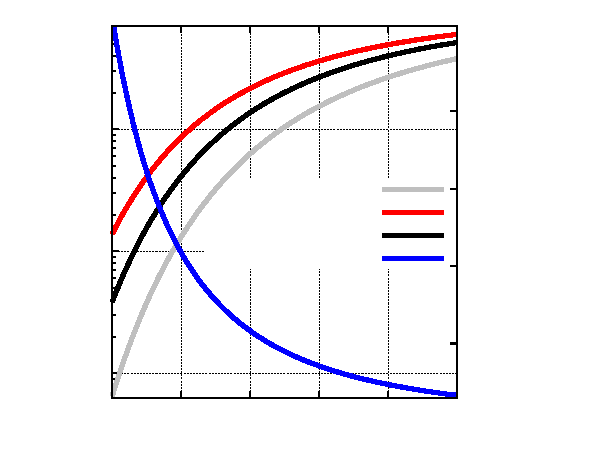
\includegraphics{EnergiesTransmissionCalibration}}%
    \gplfronttext
  \end{picture}%
\endgroup
}\label{fig:EnergiesTransmissionCalibration}}
		\subfloat[Calibrated sucrose concentration]{\resizebox{0.44\linewidth}{!}{% GNUPLOT: LaTeX picture with Postscript
\begingroup
  \makeatletter
  \providecommand\color[2][]{%
    \GenericError{(gnuplot) \space\space\space\@spaces}{%
      Package color not loaded in conjunction with
      terminal option `colourtext'%
    }{See the gnuplot documentation for explanation.%
    }{Either use 'blacktext' in gnuplot or load the package
      color.sty in LaTeX.}%
    \renewcommand\color[2][]{}%
  }%
  \providecommand\includegraphics[2][]{%
    \GenericError{(gnuplot) \space\space\space\@spaces}{%
      Package graphicx or graphics not loaded%
    }{See the gnuplot documentation for explanation.%
    }{The gnuplot epslatex terminal needs graphicx.sty or graphics.sty.}%
    \renewcommand\includegraphics[2][]{}%
  }%
  \providecommand\rotatebox[2]{#2}%
  \@ifundefined{ifGPcolor}{%
    \newif\ifGPcolor
    \GPcolortrue
  }{}%
  \@ifundefined{ifGPblacktext}{%
    \newif\ifGPblacktext
    \GPblacktextfalse
  }{}%
  % define a \g@addto@macro without @ in the name:
  \let\gplgaddtomacro\g@addto@macro
  % define empty templates for all commands taking text:
  \gdef\gplbacktext{}%
  \gdef\gplfronttext{}%
  \makeatother
  \ifGPblacktext
    % no textcolor at all
    \def\colorrgb#1{}%
    \def\colorgray#1{}%
  \else
    % gray or color?
    \ifGPcolor
      \def\colorrgb#1{\color[rgb]{#1}}%
      \def\colorgray#1{\color[gray]{#1}}%
      \expandafter\def\csname LTw\endcsname{\color{white}}%
      \expandafter\def\csname LTb\endcsname{\color{black}}%
      \expandafter\def\csname LTa\endcsname{\color{black}}%
      \expandafter\def\csname LT0\endcsname{\color[rgb]{1,0,0}}%
      \expandafter\def\csname LT1\endcsname{\color[rgb]{0,1,0}}%
      \expandafter\def\csname LT2\endcsname{\color[rgb]{0,0,1}}%
      \expandafter\def\csname LT3\endcsname{\color[rgb]{1,0,1}}%
      \expandafter\def\csname LT4\endcsname{\color[rgb]{0,1,1}}%
      \expandafter\def\csname LT5\endcsname{\color[rgb]{1,1,0}}%
      \expandafter\def\csname LT6\endcsname{\color[rgb]{0,0,0}}%
      \expandafter\def\csname LT7\endcsname{\color[rgb]{1,0.3,0}}%
      \expandafter\def\csname LT8\endcsname{\color[rgb]{0.5,0.5,0.5}}%
    \else
      % gray
      \def\colorrgb#1{\color{black}}%
      \def\colorgray#1{\color[gray]{#1}}%
      \expandafter\def\csname LTw\endcsname{\color{white}}%
      \expandafter\def\csname LTb\endcsname{\color{black}}%
      \expandafter\def\csname LTa\endcsname{\color{black}}%
      \expandafter\def\csname LT0\endcsname{\color{black}}%
      \expandafter\def\csname LT1\endcsname{\color{black}}%
      \expandafter\def\csname LT2\endcsname{\color{black}}%
      \expandafter\def\csname LT3\endcsname{\color{black}}%
      \expandafter\def\csname LT4\endcsname{\color{black}}%
      \expandafter\def\csname LT5\endcsname{\color{black}}%
      \expandafter\def\csname LT6\endcsname{\color{black}}%
      \expandafter\def\csname LT7\endcsname{\color{black}}%
      \expandafter\def\csname LT8\endcsname{\color{black}}%
    \fi
  \fi
  \setlength{\unitlength}{0.0500bp}%
  \begin{picture}(5668.00,4534.00)%
    \gplgaddtomacro\gplbacktext{%
      \csname LTb\endcsname%
      \put(814,942){\makebox(0,0)[r]{\strut{} 0}}%
      \csname LTb\endcsname%
      \put(814,1417){\makebox(0,0)[r]{\strut{} 10}}%
      \csname LTb\endcsname%
      \put(814,1892){\makebox(0,0)[r]{\strut{} 20}}%
      \csname LTb\endcsname%
      \put(814,2368){\makebox(0,0)[r]{\strut{} 30}}%
      \csname LTb\endcsname%
      \put(814,2843){\makebox(0,0)[r]{\strut{} 40}}%
      \csname LTb\endcsname%
      \put(814,3318){\makebox(0,0)[r]{\strut{} 50}}%
      \csname LTb\endcsname%
      \put(814,3794){\makebox(0,0)[r]{\strut{} 60}}%
      \csname LTb\endcsname%
      \put(814,4269){\makebox(0,0)[r]{\strut{} 70}}%
      \csname LTb\endcsname%
      \put(946,484){\makebox(0,0){\strut{} 0}}%
      \csname LTb\endcsname%
      \put(2027,484){\makebox(0,0){\strut{} 5}}%
      \csname LTb\endcsname%
      \put(3109,484){\makebox(0,0){\strut{} 10}}%
      \csname LTb\endcsname%
      \put(4190,484){\makebox(0,0){\strut{} 15}}%
      \csname LTb\endcsname%
      \put(5271,484){\makebox(0,0){\strut{} 20}}%
      \put(176,2486){\rotatebox{-270}{\makebox(0,0){\strut{}Sucrose Mass Fraction / $\%$}}}%
      \put(3108,154){\makebox(0,0){\strut{}Vertical Position / mm}}%
    }%
    \gplgaddtomacro\gplfronttext{%
      \csname LTb\endcsname%
      \put(4284,4096){\makebox(0,0)[r]{\strut{}5500 eV}}%
      \csname LTb\endcsname%
      \put(4284,3876){\makebox(0,0)[r]{\strut{}8000 eV}}%
      \csname LTb\endcsname%
      \put(4284,3656){\makebox(0,0)[r]{\strut{}10000 eV}}%
    }%
    \gplbacktext
    \put(0,0){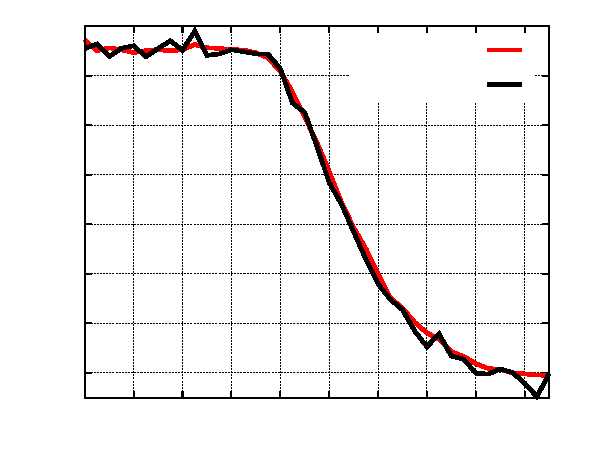
\includegraphics{SucroseTransmissionCalibration}}%
    \gplfronttext
  \end{picture}%
\endgroup
}\label{fig:SucroseTransmissionCalibration}}
	\caption{X-ray transmittance as a function of the incoming energy. a) Calculated transmittances \cite{henke_x-ray_1993} of an empty capillary, water and an aqueous sucrose mixture with 65 $\%$ mass fraction. The ratio between the water and the sucrose mixture transmittances is shown in the right axis. b) Sucrose mass fraction derived from an experimental transmittance measurement of a 65 $\%$ sucrose density gradient measured at two different energies under similiar experimental conditions. The absorbance differences are smaller for the higher energy.}

\end{figure}

However, the calculated transmission of the empty rectangular capillary is less than 1 $\%$ below 6000 eV as shown in figure \ref{fig:EnergiesTransmissionCalibration} and the filled capillary transmits 0.03 $\%$ of the incoming photon flux at 5500 eV, as observed in figure \ref{fig:KiskerTransmissionCalibration}. Therefore, a compromise between the absorbance ratio and the capillary transmittance is taken at a photon energy of 5500 eV. 

\subsection{SAXS measurements}
\label{sec:DensityGradientSAXS}

In order to collect the scattering patterns, the sample is moved in steps of 0.5 mm along the central vertical capillary axis and exposed at each position for about 1 minute. The acquisition time depends notably on the experimental parameters (e.g. sample concentration, scattering power of the material...), though it is strictly limited by the diffusion time of the contrast agent. At these positions, the solution transmittances were previously measured and the suspending medium electron density calibrated, as described previously. Due to a vertical beam size of about 0.5 mm, the measured scattering curve is an average over a range of solvent electron densities, specially relevant at the height where the density gradient is steeper. 

As a consequence of the observations from figure \ref{fig:EnergiesTransmissionCalibration}, the incident photon energy \(E = \left(8000.0  \pm 0.8\right)\) eV was chosen to be higher than the photon energy employed for the transmission measurements to improve the recorded statistics, due to a ca. 200 higher transmission \cite{henke_x-ray_1993}. The decreasing photon flux at the FCM beamline for high energies, as depicted in figure \ref{fig:FCMBeamlineFlux}, limits the photon energy used for scattering experiments up to 8800 eV.

The dimensions of the investigated particle defines the required $q$-range of the experiment, which is delimited by the incoming energy and the sample-detector distance, as discussed in section \ref{sec:SAXS_experimental}. The photon energy is limited by the needs of the sample environment, but the distance can be adjusted with the HZB-SAXS instrument to the nanoparticle requirements and can compensate the energy restriction. For sizes typically ranging from 10 to 200 nm, the sample-detector distance is fixed at 4500 mm and enables $q$-values between 0.03 and 1.1 nm$^{-1}$ at 8000 eV.

Since the equipment of the monitor diode on the beamstop in April 2016, the sample transmittance can be recorded simultaneously with the scattering patterns. The longer integration times required for the scattering experiments (around 60 s) increase the statistics of the simultaneous X-ray transmission measurement by a factor of ca. 6, improving the quality of the transmittance data. The possibility to collect the scattering data at the same photon energy that the solution transmittances improves the normalization of the scattering curve and the calibration of the solvent electron densities. Unfortunately, all the results presented in this work were recorded before the commissioning of the beamstop diode.

\section{Continuous contrast variation in SAXS on PS-COOH colloids: Proof of concept/principle}
\label{sec:KiskerResults}

In order to demonstrate the proposed technique, latex nanoparticles with a core-shell structure were measured. The particles have a narrow size distribution and consist of a spherical polystyrene (PS) core enclosed by a thin shell of a denser polymer, most likely poly(methyl methacrylate) (PMMA).

\subsection{Particles and chemicals}
Carboxylated polystyrene nanoparticles with a nominal size of 105 nm suspended in water were purchased from Kisker Biotech (Steinfurt, \emph{Germany}). The synthesis by multi-addition emulsion polymerization suggests that the assumption made in \(\S\)\textcolor{red}{GUINIER SECTION WHEN DESCRIBING THE POLYDISPERSITY IN THE FORMULA} is correct and the average density of the particle is not altered by the size polydispersity.

\textcolor{red}{HOW MUCH SUCROSE AND PARTICLE CONCENTRATION}

 particle concentration of \(12.6 \mbox{ mg/ml} \) . The dense aqueous solution was prepared with \( 21.23\,\%\) sucrose mass fraction (Sigma-Aldrich (Missouri, \emph{USA})) with a physical density of \(\rho_1=1.088 \) g/cm\(^3\), whereas a lighter one was produced without sucrose (\(\rho_2=0.997 \) g/cm\(^3\)).
 
\textcolor{red}{MAYBE NO SUB-SECTIONS.... THE CHEMICALS CAN BE DESCRIBED IN THE INTRO, BEFORE EXPLAINING THE RESULTS} 

\subsection{Results}

In total, 40 scattering curves with different solvent electron densities were measured at two different times \(t_1=\)78 min and \(t_2=\)156 min after filling the capillaries.

The measured scattering curves of the polystyrene particles are displayed in figure \ref{fig:KiskerContinuousSAXS}. In the region for \(q\) from 0.03 nm\(^{-1}\) to 0.5 nm\(^{-1}\) it is possible to observe the variation of the curve features corresponding to the particle form factor through the increase of the solvent electron density from 333.7 nm\(^{-3}\) at the top edge of the density gradient to 360.3 nm\(^{-3}\) at the maximum sucrose concentration. In this region, the experimental background is composed mainly by the contribution of the capillary scattering at the low $q$-region and the uniform scattering of the suspending medium. The experimental background scattering varies for different sucrose concentrations, but their variations are small and the background remains one order of magnitude below the sample scattering in the relevant Fourier region.

\begin{figure}%[htbp]
	\centering
		% GNUPLOT: LaTeX picture with Postscript
\begingroup
  \makeatletter
  \providecommand\color[2][]{%
    \GenericError{(gnuplot) \space\space\space\@spaces}{%
      Package color not loaded in conjunction with
      terminal option `colourtext'%
    }{See the gnuplot documentation for explanation.%
    }{Either use 'blacktext' in gnuplot or load the package
      color.sty in LaTeX.}%
    \renewcommand\color[2][]{}%
  }%
  \providecommand\includegraphics[2][]{%
    \GenericError{(gnuplot) \space\space\space\@spaces}{%
      Package graphicx or graphics not loaded%
    }{See the gnuplot documentation for explanation.%
    }{The gnuplot epslatex terminal needs graphicx.sty or graphics.sty.}%
    \renewcommand\includegraphics[2][]{}%
  }%
  \providecommand\rotatebox[2]{#2}%
  \@ifundefined{ifGPcolor}{%
    \newif\ifGPcolor
    \GPcolortrue
  }{}%
  \@ifundefined{ifGPblacktext}{%
    \newif\ifGPblacktext
    \GPblacktextfalse
  }{}%
  % define a \g@addto@macro without @ in the name:
  \let\gplgaddtomacro\g@addto@macro
  % define empty templates for all commands taking text:
  \gdef\gplbacktext{}%
  \gdef\gplfronttext{}%
  \makeatother
  \ifGPblacktext
    % no textcolor at all
    \def\colorrgb#1{}%
    \def\colorgray#1{}%
  \else
    % gray or color?
    \ifGPcolor
      \def\colorrgb#1{\color[rgb]{#1}}%
      \def\colorgray#1{\color[gray]{#1}}%
      \expandafter\def\csname LTw\endcsname{\color{white}}%
      \expandafter\def\csname LTb\endcsname{\color{black}}%
      \expandafter\def\csname LTa\endcsname{\color{black}}%
      \expandafter\def\csname LT0\endcsname{\color[rgb]{1,0,0}}%
      \expandafter\def\csname LT1\endcsname{\color[rgb]{0,1,0}}%
      \expandafter\def\csname LT2\endcsname{\color[rgb]{0,0,1}}%
      \expandafter\def\csname LT3\endcsname{\color[rgb]{1,0,1}}%
      \expandafter\def\csname LT4\endcsname{\color[rgb]{0,1,1}}%
      \expandafter\def\csname LT5\endcsname{\color[rgb]{1,1,0}}%
      \expandafter\def\csname LT6\endcsname{\color[rgb]{0,0,0}}%
      \expandafter\def\csname LT7\endcsname{\color[rgb]{1,0.3,0}}%
      \expandafter\def\csname LT8\endcsname{\color[rgb]{0.5,0.5,0.5}}%
    \else
      % gray
      \def\colorrgb#1{\color{black}}%
      \def\colorgray#1{\color[gray]{#1}}%
      \expandafter\def\csname LTw\endcsname{\color{white}}%
      \expandafter\def\csname LTb\endcsname{\color{black}}%
      \expandafter\def\csname LTa\endcsname{\color{black}}%
      \expandafter\def\csname LT0\endcsname{\color{black}}%
      \expandafter\def\csname LT1\endcsname{\color{black}}%
      \expandafter\def\csname LT2\endcsname{\color{black}}%
      \expandafter\def\csname LT3\endcsname{\color{black}}%
      \expandafter\def\csname LT4\endcsname{\color{black}}%
      \expandafter\def\csname LT5\endcsname{\color{black}}%
      \expandafter\def\csname LT6\endcsname{\color{black}}%
      \expandafter\def\csname LT7\endcsname{\color{black}}%
      \expandafter\def\csname LT8\endcsname{\color{black}}%
    \fi
  \fi
  \setlength{\unitlength}{0.0500bp}%
  \begin{picture}(5668.00,4534.00)%
    \gplgaddtomacro\gplbacktext{%
      \csname LTb\endcsname%
      \put(858,937){\makebox(0,0)[r]{\strut{} 1}}%
      \csname LTb\endcsname%
      \put(858,1986){\makebox(0,0)[r]{\strut{} 10}}%
      \csname LTb\endcsname%
      \put(858,3035){\makebox(0,0)[r]{\strut{} 100}}%
      \csname LTb\endcsname%
      \put(858,4084){\makebox(0,0)[r]{\strut{} 1000}}%
      \csname LTb\endcsname%
      \put(990,484){\makebox(0,0){\strut{} 0.03}}%
      \csname LTb\endcsname%
      \put(1615,484){\makebox(0,0){\strut{} 0.05}}%
      \csname LTb\endcsname%
      \put(2463,484){\makebox(0,0){\strut{} 0.1}}%
      \csname LTb\endcsname%
      \put(3312,484){\makebox(0,0){\strut{} 0.2}}%
      \csname LTb\endcsname%
      \put(3808,484){\makebox(0,0){\strut{} 0.3}}%
      \csname LTb\endcsname%
      \put(4433,484){\makebox(0,0){\strut{} 0.5}}%
      \put(220,2266){\rotatebox{-270}{\makebox(0,0){\strut{}Scattering Intensity / a.u.}}}%
      \put(2711,154){\makebox(0,0){\strut{}$q$ / nm$^{-1}$}}%
    }%
    \gplgaddtomacro\gplfronttext{%
      \csname LTb\endcsname%
      \put(4692,878){\makebox(0,0)[l]{\strut{}335.0}}%
      \put(4692,1548){\makebox(0,0)[l]{\strut{}340.0}}%
      \put(4692,2218){\makebox(0,0)[l]{\strut{}345.0}}%
      \put(4692,2888){\makebox(0,0)[l]{\strut{}350.0}}%
      \put(4692,3558){\makebox(0,0)[l]{\strut{}355.0}}%
      \put(4692,4228){\makebox(0,0)[l]{\strut{}360.0}}%
      \put(5418,2486){\rotatebox{-90}{\makebox(0,0){\strut{}\fsmedium Solvent Electron Density / nm$^{-3}$}}}%
    }%
    \gplbacktext
    \put(0,0){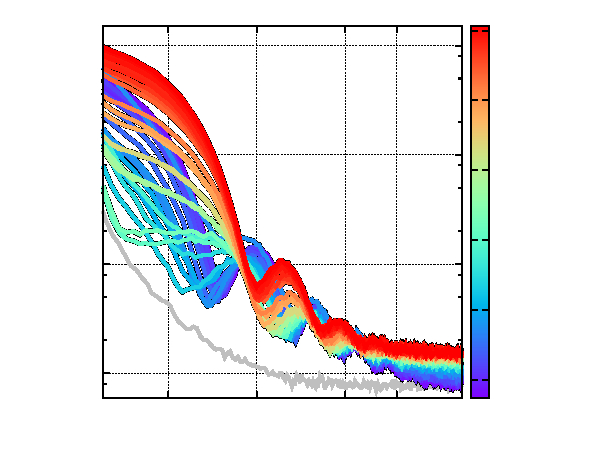
\includegraphics{KiskerContinuousSAXS}}%
    \gplfronttext
  \end{picture}%
\endgroup

		\caption{Experimental scattering curves of polystyrene nanoparticles (Kisker) for different suspending medium electron densities measured between 78 and 93 minutes after the inception of the density gradient. The dashed line shows the experimental background, containing scattering contributions from the capillary and the pure solvent.}
		\label{fig:KiskerContinuousSAXS}
\end{figure}

Upon increasing the solvent density, the position of the first minimum shifts from 0.07 nm\(^{-1}\) towards smaller \(q\)-values until it vanishes when the solvent electron density matches the average electron density of the measured particle. In the Fourier region of the scattering curves, several minima are observed which shift towards smaller \(q\)-values when increasing the solvent electron density. Upon subtracting the experimental background from the scattering curve, a decrease of the scattering intensity towards $q=0$ is observed only for the solvent electron density closest to the match point as depicted in figure \ref{fig:KiskerBackgroundSubtraction}. Therefore, background corrections can be neglected for systems with relatively high scattering power like in this study. For low-scatterers, an accurate background correction by measuring the pure suspending medium at different sucrose concentrations might be required. The behaviour at low $q$-values will be further discussed in section \S\ref{sec:guinier_analysis} when evaluating the zero-angle intensity.

\begin{figure}%[htbp]
	\centering
		% GNUPLOT: LaTeX picture with Postscript
\begingroup
  \makeatletter
  \providecommand\color[2][]{%
    \GenericError{(gnuplot) \space\space\space\@spaces}{%
      Package color not loaded in conjunction with
      terminal option `colourtext'%
    }{See the gnuplot documentation for explanation.%
    }{Either use 'blacktext' in gnuplot or load the package
      color.sty in LaTeX.}%
    \renewcommand\color[2][]{}%
  }%
  \providecommand\includegraphics[2][]{%
    \GenericError{(gnuplot) \space\space\space\@spaces}{%
      Package graphicx or graphics not loaded%
    }{See the gnuplot documentation for explanation.%
    }{The gnuplot epslatex terminal needs graphicx.sty or graphics.sty.}%
    \renewcommand\includegraphics[2][]{}%
  }%
  \providecommand\rotatebox[2]{#2}%
  \@ifundefined{ifGPcolor}{%
    \newif\ifGPcolor
    \GPcolortrue
  }{}%
  \@ifundefined{ifGPblacktext}{%
    \newif\ifGPblacktext
    \GPblacktextfalse
  }{}%
  % define a \g@addto@macro without @ in the name:
  \let\gplgaddtomacro\g@addto@macro
  % define empty templates for all commands taking text:
  \gdef\gplbacktext{}%
  \gdef\gplfronttext{}%
  \makeatother
  \ifGPblacktext
    % no textcolor at all
    \def\colorrgb#1{}%
    \def\colorgray#1{}%
  \else
    % gray or color?
    \ifGPcolor
      \def\colorrgb#1{\color[rgb]{#1}}%
      \def\colorgray#1{\color[gray]{#1}}%
      \expandafter\def\csname LTw\endcsname{\color{white}}%
      \expandafter\def\csname LTb\endcsname{\color{black}}%
      \expandafter\def\csname LTa\endcsname{\color{black}}%
      \expandafter\def\csname LT0\endcsname{\color[rgb]{1,0,0}}%
      \expandafter\def\csname LT1\endcsname{\color[rgb]{0,1,0}}%
      \expandafter\def\csname LT2\endcsname{\color[rgb]{0,0,1}}%
      \expandafter\def\csname LT3\endcsname{\color[rgb]{1,0,1}}%
      \expandafter\def\csname LT4\endcsname{\color[rgb]{0,1,1}}%
      \expandafter\def\csname LT5\endcsname{\color[rgb]{1,1,0}}%
      \expandafter\def\csname LT6\endcsname{\color[rgb]{0,0,0}}%
      \expandafter\def\csname LT7\endcsname{\color[rgb]{1,0.3,0}}%
      \expandafter\def\csname LT8\endcsname{\color[rgb]{0.5,0.5,0.5}}%
    \else
      % gray
      \def\colorrgb#1{\color{black}}%
      \def\colorgray#1{\color[gray]{#1}}%
      \expandafter\def\csname LTw\endcsname{\color{white}}%
      \expandafter\def\csname LTb\endcsname{\color{black}}%
      \expandafter\def\csname LTa\endcsname{\color{black}}%
      \expandafter\def\csname LT0\endcsname{\color{black}}%
      \expandafter\def\csname LT1\endcsname{\color{black}}%
      \expandafter\def\csname LT2\endcsname{\color{black}}%
      \expandafter\def\csname LT3\endcsname{\color{black}}%
      \expandafter\def\csname LT4\endcsname{\color{black}}%
      \expandafter\def\csname LT5\endcsname{\color{black}}%
      \expandafter\def\csname LT6\endcsname{\color{black}}%
      \expandafter\def\csname LT7\endcsname{\color{black}}%
      \expandafter\def\csname LT8\endcsname{\color{black}}%
    \fi
  \fi
  \setlength{\unitlength}{0.0500bp}%
  \begin{picture}(5668.00,4534.00)%
    \gplgaddtomacro\gplbacktext{%
      \csname LTb\endcsname%
      \put(594,1636){\makebox(0,0)[r]{\strut{} 1}}%
      \csname LTb\endcsname%
      \put(594,3419){\makebox(0,0)[r]{\strut{} 10}}%
      \csname LTb\endcsname%
      \put(1315,484){\makebox(0,0){\strut{} 0.05}}%
      \csname LTb\endcsname%
      \put(2231,484){\makebox(0,0){\strut{} 0.1}}%
      \csname LTb\endcsname%
      \put(3146,484){\makebox(0,0){\strut{} 0.2}}%
      \csname LTb\endcsname%
      \put(4356,484){\makebox(0,0){\strut{} 0.5}}%
      \csname LTb\endcsname%
      \put(5271,484){\makebox(0,0){\strut{} 1}}%
      \put(220,2266){\rotatebox{-270}{\makebox(0,0){\strut{}Scattering Intensity / a.u.}}}%
      \put(2998,154){\makebox(0,0){\strut{}$q$ / nm$^{-1}$}}%
    }%
    \gplgaddtomacro\gplfronttext{%
      \csname LTb\endcsname%
      \put(4284,4096){\makebox(0,0)[r]{\strut{}Original curve}}%
      \csname LTb\endcsname%
      \put(4284,3876){\makebox(0,0)[r]{\strut{}Water Background}}%
      \csname LTb\endcsname%
      \put(4284,3656){\makebox(0,0)[r]{\strut{}Subtracted Curve}}%
    }%
    \gplbacktext
    \put(0,0){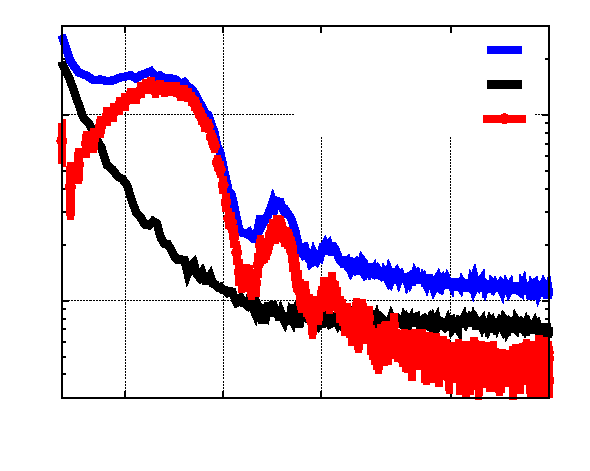
\includegraphics{KiskerBackgroundSubtraction}}%
    \gplfronttext
  \end{picture}%
\endgroup

		\caption{The thick red line shows the scattering curve measured at $\rho_{solv}$ = 345.4 nm$^{-3}$, close to the match point, and the dotted line displays the experimental background. The symbols with errorbars show the background corrected scattering curve.}
		\label{fig:KiskerBackgroundSubtraction}
\end{figure}

The presence of the clearly visible isoscattering point around \(q=0.09\) nm\(^{-1}\) confirms the existence of an inner structure. This heterogeneous composition was previously reported for the same colloids by \citet{minelli_characterization_2014}, who observed methacrylic acid (MAA) and methylmethacrylate (MMA) at the particle surface, both monomer precursors of PMMA polymerization. A more detailed insight into the radial morphology is presented subsequently, using the theoretical framework already introduced.

\section{Data evaluation}
%\section{Model dependent evaluation}
\label{sec:KiskerResultsEvaluation}

These datasets can be analysed using different, complementary evaluation methods. In this article, both a model-free theoretical framework as well as model fit are applied and, in combination, deliver a detailed insight into the inner structure of particles.


\subsection{Core-shell form factor fit}
\label{sec:coreshell_fit}
A core-shell model fit to the scattering curves is displayed in figure \ref{fig:KiskerSAXSCoreshellFit} for three representative contrasts. The model represents a radially symmetric particle, with a sharp interface between the outer shell and the inner core. This is a specific case of equation \eqref{eq:multicore-shell} with \( n=2 \)
\begin{equation}
F_{CS}(q,R,R_{core})=\Delta\eta f_{sph}(q,R)+\Delta\rho\left[ f_{sph}(q,R)-f_{sph}(q,R_{core}) \right] ,
\label{eq:ff_cs}
\end{equation}
where \(R \) and \(R_{core} \)  are the outer shell and inner core radii respectively and the excess of electron density is \(\Delta\rho=\rho_{shell}-\rho_{core}\). The simultaneous fitting of the form factor to the 40 measured scattering curves was performed by means of the method of least squares in the Fourier region \citet{pedersen_analysis_1997}. The calculated scattered intensity was modelled as the sum of the particle contributions and a two-component background \(I_{bg}=C_0+C_4q^{-\gamma} \). The parameters \(\rho_{core}\), \(\rho_{shell}\), \(R\), \(R_{core}\) and \(\gamma\) were fitted simultaneously for all curves, whilst \( C_0 \) and \( C_4 \) were adjusted independently for each solvent density. A Gaussian size distribution was assumed. For the suspending medium electron density \( \rho_{solv} \) appearing in the contrast \( \Delta\eta \), the value determined from the transmission measurement was used for each curve.

\begin{figure}%[htbp]
	\centering
		% GNUPLOT: LaTeX picture with Postscript
\begingroup
  \makeatletter
  \providecommand\color[2][]{%
    \GenericError{(gnuplot) \space\space\space\@spaces}{%
      Package color not loaded in conjunction with
      terminal option `colourtext'%
    }{See the gnuplot documentation for explanation.%
    }{Either use 'blacktext' in gnuplot or load the package
      color.sty in LaTeX.}%
    \renewcommand\color[2][]{}%
  }%
  \providecommand\includegraphics[2][]{%
    \GenericError{(gnuplot) \space\space\space\@spaces}{%
      Package graphicx or graphics not loaded%
    }{See the gnuplot documentation for explanation.%
    }{The gnuplot epslatex terminal needs graphicx.sty or graphics.sty.}%
    \renewcommand\includegraphics[2][]{}%
  }%
  \providecommand\rotatebox[2]{#2}%
  \@ifundefined{ifGPcolor}{%
    \newif\ifGPcolor
    \GPcolortrue
  }{}%
  \@ifundefined{ifGPblacktext}{%
    \newif\ifGPblacktext
    \GPblacktextfalse
  }{}%
  % define a \g@addto@macro without @ in the name:
  \let\gplgaddtomacro\g@addto@macro
  % define empty templates for all commands taking text:
  \gdef\gplbacktext{}%
  \gdef\gplfronttext{}%
  \makeatother
  \ifGPblacktext
    % no textcolor at all
    \def\colorrgb#1{}%
    \def\colorgray#1{}%
  \else
    % gray or color?
    \ifGPcolor
      \def\colorrgb#1{\color[rgb]{#1}}%
      \def\colorgray#1{\color[gray]{#1}}%
      \expandafter\def\csname LTw\endcsname{\color{white}}%
      \expandafter\def\csname LTb\endcsname{\color{black}}%
      \expandafter\def\csname LTa\endcsname{\color{black}}%
      \expandafter\def\csname LT0\endcsname{\color[rgb]{1,0,0}}%
      \expandafter\def\csname LT1\endcsname{\color[rgb]{0,1,0}}%
      \expandafter\def\csname LT2\endcsname{\color[rgb]{0,0,1}}%
      \expandafter\def\csname LT3\endcsname{\color[rgb]{1,0,1}}%
      \expandafter\def\csname LT4\endcsname{\color[rgb]{0,1,1}}%
      \expandafter\def\csname LT5\endcsname{\color[rgb]{1,1,0}}%
      \expandafter\def\csname LT6\endcsname{\color[rgb]{0,0,0}}%
      \expandafter\def\csname LT7\endcsname{\color[rgb]{1,0.3,0}}%
      \expandafter\def\csname LT8\endcsname{\color[rgb]{0.5,0.5,0.5}}%
    \else
      % gray
      \def\colorrgb#1{\color{black}}%
      \def\colorgray#1{\color[gray]{#1}}%
      \expandafter\def\csname LTw\endcsname{\color{white}}%
      \expandafter\def\csname LTb\endcsname{\color{black}}%
      \expandafter\def\csname LTa\endcsname{\color{black}}%
      \expandafter\def\csname LT0\endcsname{\color{black}}%
      \expandafter\def\csname LT1\endcsname{\color{black}}%
      \expandafter\def\csname LT2\endcsname{\color{black}}%
      \expandafter\def\csname LT3\endcsname{\color{black}}%
      \expandafter\def\csname LT4\endcsname{\color{black}}%
      \expandafter\def\csname LT5\endcsname{\color{black}}%
      \expandafter\def\csname LT6\endcsname{\color{black}}%
      \expandafter\def\csname LT7\endcsname{\color{black}}%
      \expandafter\def\csname LT8\endcsname{\color{black}}%
    \fi
  \fi
    \setlength{\unitlength}{0.0500bp}%
    \ifx\gptboxheight\undefined%
      \newlength{\gptboxheight}%
      \newlength{\gptboxwidth}%
      \newsavebox{\gptboxtext}%
    \fi%
    \setlength{\fboxrule}{0.5pt}%
    \setlength{\fboxsep}{1pt}%
\begin{picture}(5668.00,4534.00)%
    \gplgaddtomacro\gplbacktext{%
      \csname LTb\endcsname%
      \put(726,1013){\makebox(0,0)[r]{\strut{}$1$}}%
      \csname LTb\endcsname%
      \put(726,2038){\makebox(0,0)[r]{\strut{}$10$}}%
      \csname LTb\endcsname%
      \put(726,3063){\makebox(0,0)[r]{\strut{}$100$}}%
      \csname LTb\endcsname%
      \put(726,4088){\makebox(0,0)[r]{\strut{}$1000$}}%
      \csname LTb\endcsname%
      \put(1574,484){\makebox(0,0){\strut{}$0.05$}}%
      \csname LTb\endcsname%
      \put(2687,484){\makebox(0,0){\strut{}$0.1$}}%
      \csname LTb\endcsname%
      \put(3800,484){\makebox(0,0){\strut{}$0.2$}}%
      \csname LTb\endcsname%
      \put(4451,484){\makebox(0,0){\strut{}$0.3$}}%
      \csname LTb\endcsname%
      \put(5271,484){\makebox(0,0){\strut{}$0.5$}}%
    }%
    \gplgaddtomacro\gplfronttext{%
      \csname LTb\endcsname%
      \put(220,2486){\rotatebox{-270}{\makebox(0,0){\strut{}Scattering Intensity / a.u.}}}%
      \put(3064,154){\makebox(0,0){\strut{}$q$ / nm$^{-1}$}}%
      \csname LTb\endcsname%
      \put(1927,1564){\makebox(0,0)[r]{\strut{}\smaller 11.4 nm$^{-3}$}}%
      \csname LTb\endcsname%
      \put(1927,1234){\makebox(0,0)[r]{\strut{}\smaller 0.4 nm$^{-3}$}}%
      \csname LTb\endcsname%
      \put(1927,904){\makebox(0,0)[r]{\strut{}\smaller -11.2 nm$^{-3}$}}%
    }%
    \gplgaddtomacro\gplbacktext{%
      \csname LTb\endcsname%
      \put(3125,2608){\makebox(0,0)[r]{\strut{}\fssmall 330}}%
      \csname LTb\endcsname%
      \put(3125,3018){\makebox(0,0)[r]{\strut{}\fssmall 340}}%
      \csname LTb\endcsname%
      \put(3125,3427){\makebox(0,0)[r]{\strut{}\fssmall 350}}%
      \csname LTb\endcsname%
      \put(3125,3837){\makebox(0,0)[r]{\strut{}\fssmall 360}}%
      \csname LTb\endcsname%
      \put(3257,2388){\makebox(0,0){\strut{}\fssmall 0}}%
      \csname LTb\endcsname%
      \put(3601,2388){\makebox(0,0){\strut{}\fssmall 10}}%
      \csname LTb\endcsname%
      \put(3944,2388){\makebox(0,0){\strut{}\fssmall 20}}%
      \csname LTb\endcsname%
      \put(4288,2388){\makebox(0,0){\strut{}\fssmall 30}}%
      \csname LTb\endcsname%
      \put(4632,2388){\makebox(0,0){\strut{}\fssmall 40}}%
      \csname LTb\endcsname%
      \put(4975,2388){\makebox(0,0){\strut{}\fssmall 50}}%
    }%
    \gplgaddtomacro\gplfronttext{%
      \csname LTb\endcsname%
      \put(2619,3391){\rotatebox{-270}{\makebox(0,0){\strut{}\fssmall{Electron Density / nm$^{-3}$}}}}%
      \put(4150,2058){\makebox(0,0){\strut{}\fssmall{$R$} / nm}}%
    }%
    \gplbacktext
    \put(0,0){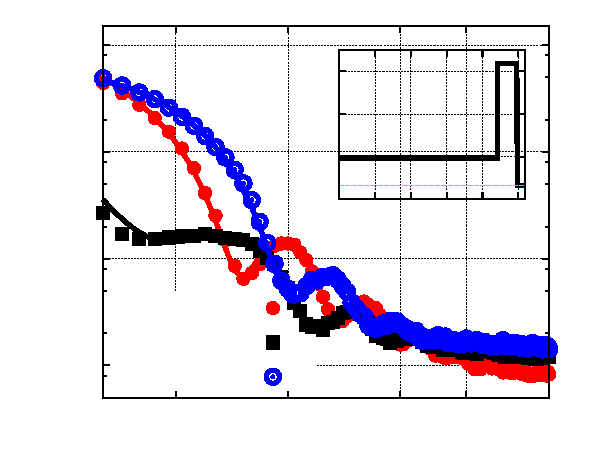
\includegraphics{KiskerSAXSCoreshellFit}}%
    \gplfronttext
  \end{picture}%
\endgroup

		\caption{ The simulated scattering curves from the core-shell model fit at three selected contrasts $\rho_0-\rho_{solv}$ are shown as lines together with the experimental data points. In the inset, the electron density profile corresponding to the fitted core-shell form factor is displayed.}
		\label{fig:KiskerSAXSCoreshellFit}
\end{figure}

The obtained results are \(R=\left(49.7 \pm 2.8\right) \) nm, \(R_{core}=\left(44.2 \pm 0.9\right) \) nm, \(\rho_{core}=\left(339.7 \pm 0.1\right)\) nm\(^{-3}\) and \(\rho_{shell}=\left(361.9 \pm 2.0\right)\) nm\(^{-3}\), which represent the radial structure of a dense, thin shell surrounding a lighter core, as seen in the inset of figure \ref{fig:KiskerSAXSCoreshellFit}. The resulting average electron density of the particle is \(\rho_{0}=\left(345.9 \pm 1.5\right)\) nm\(^{-3}\) and the polydispersity degree, \(p_d=\left(22.8\pm 6.0\right)\,\%\). The best fitting background corresponds to a value of \( \gamma = 4.3\pm 0.5 \), close to the case \( \gamma = 4 \) originating from large impurities or precipitates \citet{pedersen_determination_1994}. The fit uncertainty was calculated with a confidence interval of one standard deviation. 

It is noticeable that the calculated electron density of the core coincides exactly with the theoretical polystyrene electron density, although the electron density of the shell is remarkably lower than the theoretical value of 383.4 nm\(^{-3}\) for PMMA \citet{ballauff_saxs_2001-1}. This might arise from the lower density of the monomers used in the particle synthesis (MAA and MMA), which could have mixed with the styrene monomers resulting in a less dense material than PMMA. This model might present some differences with the real colloid system, as a diffusive interfacial layer can be expected between polymer phases in colloids \citet{dingenouts_interface_1994}, especially for incompatible polymers such as PMMA and PS. On the other hand, the large quantity of scattering curves used for the fitting process and, accordingly, the decreased uncertainty suggests that the chosen sharp core-shell model has a great resemblance to the real particle.

%\section{Model-free approach to contrast variation data}
\subsection{Isoscattering point}
\subsubsection{Quantification: Relative standard deviation}
The first isoscattering point is clearly visible in figure \ref{fig:KiskerContinuousSAXS}. For a more quantitative evaluation, the relative standard deviation of the 40 measured curves at each \(q\) is calculated according to
\begin{equation}
\sigma_r (q)=\frac{1}{\bar{I}(q)}\sqrt{\frac{\sum^{M}_{i=1} (I_i(q) -\bar{I} (q))^2 }{M-1}} ,
\end{equation}
where \(\bar{I} (q)\) is the mean value of the intensity at \(q\) and \( M \) is the number of scattering curves. This value becomes minimal at an isoscattering point. In order to reduce the influence of outliers, a truncated mean value was utilized, disregarding the \(10\,\%\) most dispersed data points. In figure \ref{fig:KiskerIsopoint}, the relative standard deviation is plotted as a function of the momentum transfer \(q\), which shows several distinguishable minima corresponding to isoscattering points.

\begin{figure}%[htbp]
	\centering
		% GNUPLOT: LaTeX picture with Postscript
\begingroup
  \makeatletter
  \providecommand\color[2][]{%
    \GenericError{(gnuplot) \space\space\space\@spaces}{%
      Package color not loaded in conjunction with
      terminal option `colourtext'%
    }{See the gnuplot documentation for explanation.%
    }{Either use 'blacktext' in gnuplot or load the package
      color.sty in LaTeX.}%
    \renewcommand\color[2][]{}%
  }%
  \providecommand\includegraphics[2][]{%
    \GenericError{(gnuplot) \space\space\space\@spaces}{%
      Package graphicx or graphics not loaded%
    }{See the gnuplot documentation for explanation.%
    }{The gnuplot epslatex terminal needs graphicx.sty or graphics.sty.}%
    \renewcommand\includegraphics[2][]{}%
  }%
  \providecommand\rotatebox[2]{#2}%
  \@ifundefined{ifGPcolor}{%
    \newif\ifGPcolor
    \GPcolortrue
  }{}%
  \@ifundefined{ifGPblacktext}{%
    \newif\ifGPblacktext
    \GPblacktextfalse
  }{}%
  % define a \g@addto@macro without @ in the name:
  \let\gplgaddtomacro\g@addto@macro
  % define empty templates for all commands taking text:
  \gdef\gplbacktext{}%
  \gdef\gplfronttext{}%
  \makeatother
  \ifGPblacktext
    % no textcolor at all
    \def\colorrgb#1{}%
    \def\colorgray#1{}%
  \else
    % gray or color?
    \ifGPcolor
      \def\colorrgb#1{\color[rgb]{#1}}%
      \def\colorgray#1{\color[gray]{#1}}%
      \expandafter\def\csname LTw\endcsname{\color{white}}%
      \expandafter\def\csname LTb\endcsname{\color{black}}%
      \expandafter\def\csname LTa\endcsname{\color{black}}%
      \expandafter\def\csname LT0\endcsname{\color[rgb]{1,0,0}}%
      \expandafter\def\csname LT1\endcsname{\color[rgb]{0,1,0}}%
      \expandafter\def\csname LT2\endcsname{\color[rgb]{0,0,1}}%
      \expandafter\def\csname LT3\endcsname{\color[rgb]{1,0,1}}%
      \expandafter\def\csname LT4\endcsname{\color[rgb]{0,1,1}}%
      \expandafter\def\csname LT5\endcsname{\color[rgb]{1,1,0}}%
      \expandafter\def\csname LT6\endcsname{\color[rgb]{0,0,0}}%
      \expandafter\def\csname LT7\endcsname{\color[rgb]{1,0.3,0}}%
      \expandafter\def\csname LT8\endcsname{\color[rgb]{0.5,0.5,0.5}}%
    \else
      % gray
      \def\colorrgb#1{\color{black}}%
      \def\colorgray#1{\color[gray]{#1}}%
      \expandafter\def\csname LTw\endcsname{\color{white}}%
      \expandafter\def\csname LTb\endcsname{\color{black}}%
      \expandafter\def\csname LTa\endcsname{\color{black}}%
      \expandafter\def\csname LT0\endcsname{\color{black}}%
      \expandafter\def\csname LT1\endcsname{\color{black}}%
      \expandafter\def\csname LT2\endcsname{\color{black}}%
      \expandafter\def\csname LT3\endcsname{\color{black}}%
      \expandafter\def\csname LT4\endcsname{\color{black}}%
      \expandafter\def\csname LT5\endcsname{\color{black}}%
      \expandafter\def\csname LT6\endcsname{\color{black}}%
      \expandafter\def\csname LT7\endcsname{\color{black}}%
      \expandafter\def\csname LT8\endcsname{\color{black}}%
    \fi
  \fi
  \setlength{\unitlength}{0.0500bp}%
  \begin{picture}(5668.00,4534.00)%
    \gplgaddtomacro\gplbacktext{%
      \csname LTb\endcsname%
      \put(946,1439){\makebox(0,0)[r]{\strut{} 0.1}}%
      \csname LTb\endcsname%
      \put(946,2291){\makebox(0,0)[r]{\strut{} 0.2}}%
      \csname LTb\endcsname%
      \put(946,3417){\makebox(0,0)[r]{\strut{} 0.5}}%
      \csname LTb\endcsname%
      \put(946,4269){\makebox(0,0)[r]{\strut{} 1}}%
      \csname LTb\endcsname%
      \put(1078,484){\makebox(0,0){\strut{} 0.07}}%
      \csname LTb\endcsname%
      \put(1839,484){\makebox(0,0){\strut{} 0.1}}%
      \csname LTb\endcsname%
      \put(3317,484){\makebox(0,0){\strut{} 0.2}}%
      \csname LTb\endcsname%
      \put(5271,484){\makebox(0,0){\strut{} 0.5}}%
      \put(176,2486){\rotatebox{-270}{\makebox(0,0){\strut{}Rel. Std. Deviation}}}%
      \put(3174,154){\makebox(0,0){\strut{}$q$ / nm$^{-1}$}}%
      \put(1225,1611){\makebox(0,0)[l]{\strut{}$q^{\star}_1$}}%
      \put(2315,1439){\makebox(0,0)[l]{\strut{}$q^{\star}_2$}}%
      \put(3092,1239){\makebox(0,0)[l]{\strut{}$q^{\star}_3$}}%
      \put(4252,1439){\makebox(0,0)[l]{\strut{}$q^{\star}_4$}}%
      \put(4600,1808){\makebox(0,0)[l]{\strut{}$q^{\star}_5$}}%
    }%
    \gplgaddtomacro\gplfronttext{%
    }%
    \gplbacktext
    \put(0,0){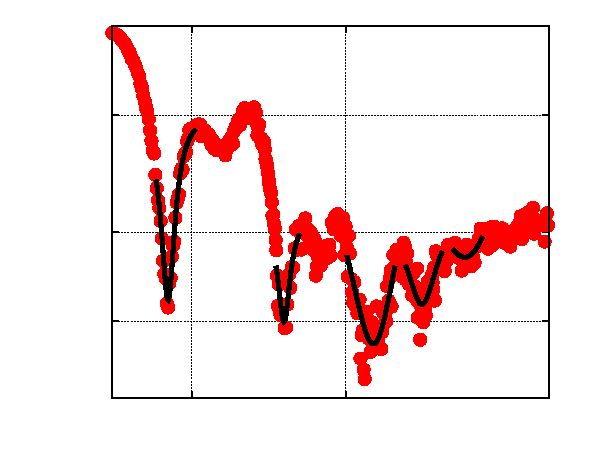
\includegraphics{KiskerIsopoint}}%
    \gplfronttext
  \end{picture}%
\endgroup

		\caption{Relative standard deviation of the scattering curves as a function of the momentum transfer. The labelled minima correspond to the first five isoscattering point positions calculated by fitting a Lorentzian function (red line).}
		\label{fig:KiskerIsopoint}
\end{figure}

\begin{table}
\caption{Experimentally determined position of the first five isoscattering points and the corresponding external particle radius $R$.}
\begin{tabular}{l|cc}
 & \( q^{\star} \) (nm\(^{-1}\))    &  \(R\) (nm) \\
\hline
 \(q^{\star}_1\) &  0.0900 & 49.9 \\
 \(q^{\star}_2\) &  0.1516 & 51.0  \\
 \(q^{\star}_3\) &  0.2267 & 48.1   \\
 \(q^{\star}_4\) &  0.2822 & 49.9    \\
 \(q^{\star}_5\) &  0.3421 & 50.3     \\
\end{tabular}
\label{tab:isopoint_Kisker}
\end{table}

A precise determination of the isoscattering point positions is performed by fitting Lorentzian functions to the minima in the relative standard deviation plot, which allows the calculation of the model-free external radius of the particle by means of equation \eqref{eq:isoscattering}. The results are presented in table \ref{tab:isopoint_Kisker}. The obtained particle radii vary in the range from \(48.1\) nm to \(51.0\) nm, although as predicted by \cite{kawaguchi_isoscattering_1992} for a polydisperse system, the isoscattering points get smeared out for larger \( q \)-values and the precision decreases, simultaneously with the increase of the solvent background at higher \(q\)-values. This can be directly observed in the quality of the experimental data, as the first two minima are clearly pronounced, while the subsequent minima appear smeared out. For instance, the isoscattering point \(q^{\star}_5\) is already too weak for an accurate evaluation and the third minimum shows two remarkably close smaller minima which might affect the shape of the function. Therefore, \(q^{\star}_1\) and \(q^{\star}_2\) yield the most reliable values for evaluating the external radius of the particles, although all results are presented in table \ref{tab:isopoint_Kisker}. The value derived from the isoscattering points \(R=50.5\) nm differs by only \(1.6\,\%\) from the radius calculated from the model fit in the previous section.

Due to the ambiguous definition of the isoscattering point diffuseness, a quantitative determination of the polydispersity of the suspended nanoparticles by means of the Lorentzian profile is rather challenging. Nevertheless, the narrow size distribution of the sample becomes clear by comparing the relative standard deviation values of the observed minima in figure \ref{fig:KiskerIsopoint} with a simulation using the structural parameters obtained in section \S\ref{sec:coreshell_fit}. The value \( \sigma_r(q^{\star}_1)=0.11 \) corresponds to a calculated ensemble polydispersity of \(24\,\% \). This value serves as an upper \( p_d \) limit due to the possible overestimation caused by the scattering contribution of the suspending medium.


\subsection{Guinier region}
\label{sec:guinier_analysis}
By analyzing the low \(q \)-region of the scattering curves, the so-called Guinier region, two important parameters can be obtained: the radius of gyration \(R_g\) and the intensity at zero angle \(I(0)\). According to \cite{feigin_structure_1987}, the fit of equation \eqref{eq:guinier} to the Guinier region is mainly valid up to \( qR_g<1.3 \). In this restricted \(q\)-range, too few data points are available for a reliable data analysis. Therefore, an extrapolation using the spherical form factor \( f_{sph}(q,R) \) over the range available before the first minimum has been employed instead to obtain \(R_g\) and \(I(0)\).

As described in \(\S\)\textcolor{red}{GUINIER THEORY CHAPTER}, the radius of gyration of a heterogeneous particle in a contrast variation experiment should behave according to equation \eqref{eq:gyration}. In figure \ref{fig:KiskerGuinierRadius}, the experimental squared radius of gyration is displayed as a function of the suspending medium electron density. The best fit to the measured data with values \(\rho_0=343.7\) nm\(^{-3}\), \( \tilde R_{g,c}=39.0\) nm, \(\tilde \alpha=4470\) nm\(^{-1}\) and \(\tilde\beta=0\) nm\(^{-4}\) is shown by the solid line. 

\begin{figure}%[htbp]
	\centering
		% GNUPLOT: LaTeX picture with Postscript
\begingroup
  \makeatletter
  \providecommand\color[2][]{%
    \GenericError{(gnuplot) \space\space\space\@spaces}{%
      Package color not loaded in conjunction with
      terminal option `colourtext'%
    }{See the gnuplot documentation for explanation.%
    }{Either use 'blacktext' in gnuplot or load the package
      color.sty in LaTeX.}%
    \renewcommand\color[2][]{}%
  }%
  \providecommand\includegraphics[2][]{%
    \GenericError{(gnuplot) \space\space\space\@spaces}{%
      Package graphicx or graphics not loaded%
    }{See the gnuplot documentation for explanation.%
    }{The gnuplot epslatex terminal needs graphicx.sty or graphics.sty.}%
    \renewcommand\includegraphics[2][]{}%
  }%
  \providecommand\rotatebox[2]{#2}%
  \@ifundefined{ifGPcolor}{%
    \newif\ifGPcolor
    \GPcolortrue
  }{}%
  \@ifundefined{ifGPblacktext}{%
    \newif\ifGPblacktext
    \GPblacktextfalse
  }{}%
  % define a \g@addto@macro without @ in the name:
  \let\gplgaddtomacro\g@addto@macro
  % define empty templates for all commands taking text:
  \gdef\gplbacktext{}%
  \gdef\gplfronttext{}%
  \makeatother
  \ifGPblacktext
    % no textcolor at all
    \def\colorrgb#1{}%
    \def\colorgray#1{}%
  \else
    % gray or color?
    \ifGPcolor
      \def\colorrgb#1{\color[rgb]{#1}}%
      \def\colorgray#1{\color[gray]{#1}}%
      \expandafter\def\csname LTw\endcsname{\color{white}}%
      \expandafter\def\csname LTb\endcsname{\color{black}}%
      \expandafter\def\csname LTa\endcsname{\color{black}}%
      \expandafter\def\csname LT0\endcsname{\color[rgb]{1,0,0}}%
      \expandafter\def\csname LT1\endcsname{\color[rgb]{0,1,0}}%
      \expandafter\def\csname LT2\endcsname{\color[rgb]{0,0,1}}%
      \expandafter\def\csname LT3\endcsname{\color[rgb]{1,0,1}}%
      \expandafter\def\csname LT4\endcsname{\color[rgb]{0,1,1}}%
      \expandafter\def\csname LT5\endcsname{\color[rgb]{1,1,0}}%
      \expandafter\def\csname LT6\endcsname{\color[rgb]{0,0,0}}%
      \expandafter\def\csname LT7\endcsname{\color[rgb]{1,0.3,0}}%
      \expandafter\def\csname LT8\endcsname{\color[rgb]{0.5,0.5,0.5}}%
    \else
      % gray
      \def\colorrgb#1{\color{black}}%
      \def\colorgray#1{\color[gray]{#1}}%
      \expandafter\def\csname LTw\endcsname{\color{white}}%
      \expandafter\def\csname LTb\endcsname{\color{black}}%
      \expandafter\def\csname LTa\endcsname{\color{black}}%
      \expandafter\def\csname LT0\endcsname{\color{black}}%
      \expandafter\def\csname LT1\endcsname{\color{black}}%
      \expandafter\def\csname LT2\endcsname{\color{black}}%
      \expandafter\def\csname LT3\endcsname{\color{black}}%
      \expandafter\def\csname LT4\endcsname{\color{black}}%
      \expandafter\def\csname LT5\endcsname{\color{black}}%
      \expandafter\def\csname LT6\endcsname{\color{black}}%
      \expandafter\def\csname LT7\endcsname{\color{black}}%
      \expandafter\def\csname LT8\endcsname{\color{black}}%
    \fi
  \fi
  \setlength{\unitlength}{0.0500bp}%
  \begin{picture}(5668.00,4534.00)%
    \gplgaddtomacro\gplbacktext{%
      \csname LTb\endcsname%
      \put(1078,704){\makebox(0,0)[r]{\strut{} 500}}%
      \csname LTb\endcsname%
      \put(1078,1341){\makebox(0,0)[r]{\strut{} 1000}}%
      \csname LTb\endcsname%
      \put(1078,1977){\makebox(0,0)[r]{\strut{} 1500}}%
      \csname LTb\endcsname%
      \put(1078,2614){\makebox(0,0)[r]{\strut{} 2000}}%
      \csname LTb\endcsname%
      \put(1078,3250){\makebox(0,0)[r]{\strut{} 2500}}%
      \csname LTb\endcsname%
      \put(1078,3887){\makebox(0,0)[r]{\strut{} 3000}}%
      \csname LTb\endcsname%
      \put(1210,484){\makebox(0,0){\strut{} 330}}%
      \csname LTb\endcsname%
      \put(1718,484){\makebox(0,0){\strut{} 335}}%
      \csname LTb\endcsname%
      \put(2225,484){\makebox(0,0){\strut{} 340}}%
      \csname LTb\endcsname%
      \put(2733,484){\makebox(0,0){\strut{} 345}}%
      \csname LTb\endcsname%
      \put(3241,484){\makebox(0,0){\strut{} 350}}%
      \csname LTb\endcsname%
      \put(3748,484){\makebox(0,0){\strut{} 355}}%
      \csname LTb\endcsname%
      \put(4256,484){\makebox(0,0){\strut{} 360}}%
      \csname LTb\endcsname%
      \put(4763,484){\makebox(0,0){\strut{} 365}}%
      \csname LTb\endcsname%
      \put(5271,484){\makebox(0,0){\strut{} 370}}%
      \put(176,2486){\rotatebox{-270}{\makebox(0,0){\strut{}$R_g^2$ / nm$^2$}}}%
      \put(3240,154){\makebox(0,0){\strut{}Solvent electron density / nm$^{-3}$}}%
      \put(2733,3887){\makebox(0,0)[l]{\strut{}$\rho_0$}}%
      \put(4763,2232){\makebox(0,0)[l]{\strut{}$\tilde R^2_{g,c}$}}%
    }%
    \gplgaddtomacro\gplfronttext{%
    }%
    \gplbacktext
    \put(0,0){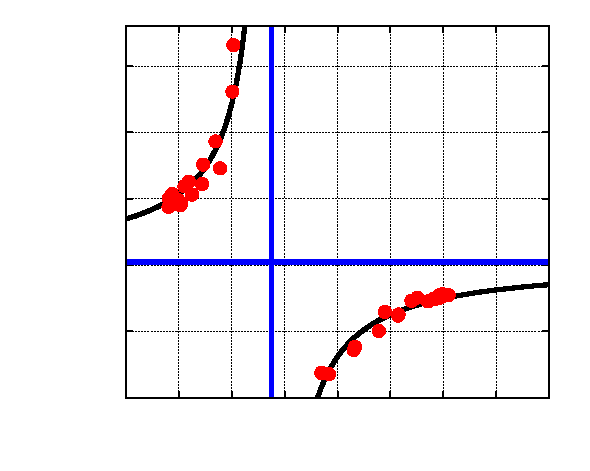
\includegraphics{KiskerGuinierRadius}}%
    \gplfronttext
  \end{picture}%
\endgroup

		\caption{Experimental squared radius of gyration as a function of the solvent electron density. Equation (6) is fitted to the data and shown as a thick line. The vertical and horizontal asymptotes correspond to $\rho_0$ and $\tilde R^2_{g,c}$ respectively.}
		\label{fig:KiskerGuinierRadius}
\end{figure}

The positive value of \(\tilde\alpha\) validates the hypothesis that a more dense polymer (probably PMMA) surrounds a lighter core (PS) \cite{stuhrmann_small-angle_2008}. The calculated average electron density of the particle \(\rho_0\) suggests a very thin layer of PMMA shell around the PS core, due to the proximity of its value to the polystyrene electron density (339.7 nm\(^{-3}\) ). The value of \( \tilde\beta=0\) proves a concentric model, where core and shell share the same centre. Using the same polydispersity value of \(22.8\,\%\) obtained in the fitting process, the value for the particle shape radius of gyration results in \(R_{g,c}=36.9\) nm and the external radius of the particle can be calculated assuming the particle as a spherical object (\( R_g^2=\frac{3}{5}R^2 \)). This calculation gives \( R=47.6\) nm, which is only 2.1 nm smaller than the calculated external radius \(R=49.7\) nm, though it might be underestimated due to the choice of a possibly inflated polydispersity. 

\subsubsection{Average electron density}
Using the same set of 40 scattering curves, the behaviour of the zero-angle intensity under the contrast variation is also investigated by fitting equation \eqref{eq:I0} to the experimental \(I(0)\), as depicted in figure \ref{fig:KiskerIntensityParabola}. A minimum in the curve is observed at \(\rho_{solv}=346.0\) nm\(^{-3}\), which corresponds to the value of the average electron density of the particle. This value is in very good agreement with the result obtained by fitting the core-shell form factor. It is also noticeable that the minimum intensity is approximately 0, which means that the effective average density of the ensemble is equal to the average density of the particle \cite{avdeev_contrast_2007}. This result further legitimates the previously made assumption that the ratio between the particle components' volumes is constant independent of the polydispersity and hence \(  \tilde \rho_0 = \rho_0  \).

\begin{figure}%[htbp]
	\centering
		% GNUPLOT: LaTeX picture with Postscript
\begingroup
  \makeatletter
  \providecommand\color[2][]{%
    \GenericError{(gnuplot) \space\space\space\@spaces}{%
      Package color not loaded in conjunction with
      terminal option `colourtext'%
    }{See the gnuplot documentation for explanation.%
    }{Either use 'blacktext' in gnuplot or load the package
      color.sty in LaTeX.}%
    \renewcommand\color[2][]{}%
  }%
  \providecommand\includegraphics[2][]{%
    \GenericError{(gnuplot) \space\space\space\@spaces}{%
      Package graphicx or graphics not loaded%
    }{See the gnuplot documentation for explanation.%
    }{The gnuplot epslatex terminal needs graphicx.sty or graphics.sty.}%
    \renewcommand\includegraphics[2][]{}%
  }%
  \providecommand\rotatebox[2]{#2}%
  \@ifundefined{ifGPcolor}{%
    \newif\ifGPcolor
    \GPcolortrue
  }{}%
  \@ifundefined{ifGPblacktext}{%
    \newif\ifGPblacktext
    \GPblacktextfalse
  }{}%
  % define a \g@addto@macro without @ in the name:
  \let\gplgaddtomacro\g@addto@macro
  % define empty templates for all commands taking text:
  \gdef\gplbacktext{}%
  \gdef\gplfronttext{}%
  \makeatother
  \ifGPblacktext
    % no textcolor at all
    \def\colorrgb#1{}%
    \def\colorgray#1{}%
  \else
    % gray or color?
    \ifGPcolor
      \def\colorrgb#1{\color[rgb]{#1}}%
      \def\colorgray#1{\color[gray]{#1}}%
      \expandafter\def\csname LTw\endcsname{\color{white}}%
      \expandafter\def\csname LTb\endcsname{\color{black}}%
      \expandafter\def\csname LTa\endcsname{\color{black}}%
      \expandafter\def\csname LT0\endcsname{\color[rgb]{1,0,0}}%
      \expandafter\def\csname LT1\endcsname{\color[rgb]{0,1,0}}%
      \expandafter\def\csname LT2\endcsname{\color[rgb]{0,0,1}}%
      \expandafter\def\csname LT3\endcsname{\color[rgb]{1,0,1}}%
      \expandafter\def\csname LT4\endcsname{\color[rgb]{0,1,1}}%
      \expandafter\def\csname LT5\endcsname{\color[rgb]{1,1,0}}%
      \expandafter\def\csname LT6\endcsname{\color[rgb]{0,0,0}}%
      \expandafter\def\csname LT7\endcsname{\color[rgb]{1,0.3,0}}%
      \expandafter\def\csname LT8\endcsname{\color[rgb]{0.5,0.5,0.5}}%
    \else
      % gray
      \def\colorrgb#1{\color{black}}%
      \def\colorgray#1{\color[gray]{#1}}%
      \expandafter\def\csname LTw\endcsname{\color{white}}%
      \expandafter\def\csname LTb\endcsname{\color{black}}%
      \expandafter\def\csname LTa\endcsname{\color{black}}%
      \expandafter\def\csname LT0\endcsname{\color{black}}%
      \expandafter\def\csname LT1\endcsname{\color{black}}%
      \expandafter\def\csname LT2\endcsname{\color{black}}%
      \expandafter\def\csname LT3\endcsname{\color{black}}%
      \expandafter\def\csname LT4\endcsname{\color{black}}%
      \expandafter\def\csname LT5\endcsname{\color{black}}%
      \expandafter\def\csname LT6\endcsname{\color{black}}%
      \expandafter\def\csname LT7\endcsname{\color{black}}%
      \expandafter\def\csname LT8\endcsname{\color{black}}%
    \fi
  \fi
  \setlength{\unitlength}{0.0500bp}%
  \begin{picture}(5668.00,4534.00)%
    \gplgaddtomacro\gplbacktext{%
      \csname LTb\endcsname%
      \put(946,841){\makebox(0,0)[r]{\strut{} 0}}%
      \csname LTb\endcsname%
      \put(946,1298){\makebox(0,0)[r]{\strut{} 0.2}}%
      \csname LTb\endcsname%
      \put(946,1755){\makebox(0,0)[r]{\strut{} 0.4}}%
      \csname LTb\endcsname%
      \put(946,2212){\makebox(0,0)[r]{\strut{} 0.6}}%
      \csname LTb\endcsname%
      \put(946,2669){\makebox(0,0)[r]{\strut{} 0.8}}%
      \csname LTb\endcsname%
      \put(946,3126){\makebox(0,0)[r]{\strut{} 1}}%
      \csname LTb\endcsname%
      \put(946,3583){\makebox(0,0)[r]{\strut{} 1.2}}%
      \csname LTb\endcsname%
      \put(946,4040){\makebox(0,0)[r]{\strut{} 1.4}}%
      \csname LTb\endcsname%
      \put(1378,484){\makebox(0,0){\strut{} 335}}%
      \csname LTb\endcsname%
      \put(2126,484){\makebox(0,0){\strut{} 340}}%
      \csname LTb\endcsname%
      \put(2875,484){\makebox(0,0){\strut{} 345}}%
      \csname LTb\endcsname%
      \put(3624,484){\makebox(0,0){\strut{} 350}}%
      \csname LTb\endcsname%
      \put(4373,484){\makebox(0,0){\strut{} 355}}%
      \csname LTb\endcsname%
      \put(5121,484){\makebox(0,0){\strut{} 360}}%
      \put(176,2486){\rotatebox{-270}{\makebox(0,0){\strut{}$I(0)$ / a.u.}}}%
      \put(3174,154){\makebox(0,0){\strut{}Solvent electron density / nm$^{-3}$}}%
    }%
    \gplgaddtomacro\gplfronttext{%
    }%
    \gplbacktext
    \put(0,0){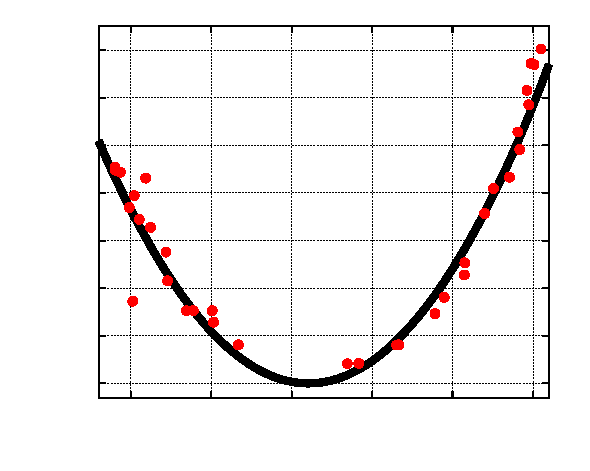
\includegraphics{KiskerIntensityParabola}}%
    \gplfronttext
  \end{picture}%
\endgroup

		\caption{Experimental zero-angle intensity as a function of the solvent electron density. The function corresponding to equation (7) is fitted to the data and shown as a thick line. The minimum in the parabola corresponds to $\rho_{solv}=\rho_0$.}
		\label{fig:KiskerIntensityParabola}
\end{figure}

\begin{itemize}
	\item [First point] Comparison of accuracy
	\item [Extrapolatio] Using just the Guinier region or extrapolating from first minimum
\end{itemize}

\section{Summary}
\label{sec:KiskerResultsSummary}
Table \ref{tab:comparison_results_Kisker} summarizes the results of all three presented methods. From the first two isoscattering points, values for the external radius and an upper bound to the polydispersity degree have been derived. Focusing on the Guinier region of the scattering curves, a value for the average electron density of the particles is found using the radius of gyration as well as the zero-angle intensity, the values of which differ by 2.3 nm\(^{-3}\). By fitting a core-shell model, an external radius of \(R=49.7\) nm and an average electron density \(\rho_0=345.9\) nm\(^{-3}\) have been obtained, which are in considerable agreement with the previous results, i.e., the values determined by the other methods are included in their confidence ranges, except for the \(\rho_0\) calculated with the radii of gyration.

\begin{table}
\caption{Comparison of the different methods presented in this article to evaluate SAXS contrast variation data.}
\begin{tabular}{l|ccc}
 & \( R\) (nm)    & \(\rho_0\) (nm\(^{-3}\)) & \(p_d\) (\(\%\))\\
\hline
 Core-shell fitting &  49.7\(\pm 2.8\)   &     345.9\(\pm 1.5\)      & 22.8\(\pm 6.0\) \\
 Isoscattering point* &  50.5 &     -          & $<24$  \\
 Radius of gyration &  47.6**      &     343.7      & -    \\
 Zero-angle intensity &  -    &     346.0      & -    \\ \hline
\multicolumn{4}{r}{*Mean value of \(q^{\star}_1\) and \(q^{\star}_2\)}\\  
\multicolumn{4}{r}{**Using the polydispersity degree from the core-shell model fitting}\\ 
\end{tabular}
\label{tab:comparison_results_Kisker}
\end{table}

From these results, it is evident that the radius of gyration interpretation produces the most deviant values. This might be founded in the complicated function fitted to the data and the reduced availability of $q$-range employed to obtain \( R_g \).

The resulting polydispersity degree of the measured particles from the model fit is in agreement with the upper limit obtained with the radii of gyration. Nevertheless the polydispersity is the parameter determined with the largest uncertainty in the fitting process and therefore this result must be considered with care.

It can be concluded that the different approaches show consistent and complementary results about the size distribution of nanoparticles with radial inner structure, especially for the external radius of the particle and its average electron density. A precise value for the polydispersity degree could not be obtained as explained previously, although a credible upper limit to the polydispersity degree of $24\,\%$ could be given.

This article demonstrates that it is possible to perform continuous contrast variation for light nanoparticles by means of a density gradient and to collect a large quantity of SAXS curves, which can be analyzed with complementary approaches to reveal a consistent insight into the size distribution and the inner structure of the suspended nanoparticles. 

By means of a model-free analysis of the experimental data based on the isoscattering point theory, an average particle diameter of 101 nm was obtained. The analysis of the Guinier region of the scattering curves shows that the radial inner structure of the particles consists of a thin, more dense layer coating the polystyrene core. Complementing these results, a core-shell model fit showed that the core component of the particle had exactly the same electron density expected for polystyrene and the shell was composed of a compound with a density below that of PMMA. This core-shell structure was expected for chemical reasons due to the different hydrophobicity of PS compared to MMA and MAA.

\textcolor{blue}{Considering the similar electronic composition of these polymers and the average electron density of the particle $\rho_0=346$ nm\(^{-3}\), an average physical density of the particles of $\rho=1.07$ g/cm\(^{3}\) can be calculated. The precision in the determination of this density proves this technique as a useful tool and an alternative to other techniques like isopycnic centrifugation \cite{vauthier_measurement_1999,arnold_sorting_2006,sun_separation_2009}, widely used with biomacromolecules.}

\subsubsection{Applicability of the technique}

The accessible electron density range is the most decisive factor to choose the contrast agent. With saccharides like sucrose or fructose, high concentrated mixtures with low viscosity can be achieved, reaching electron densities up to 400 nm$^{-3}$. Sugars are suitable for contrast variation experiments with bio-materials and polymeric nanoparticles, whose densities typically range between 0.9 and 1.4 g cm$^{-3}$. On the other hand, contrast agents like ethanol can reduce the electron density of the suspending medium until 270 nm$^{-3}$ and, besides, is perfectly miscible with water. A wide variety of biological particles exist within the available density range achieved between ethanol and sugar.

More dense solutions prepared with heavy salts (e.g. sodium polytungstate (3Na$_2$WO$_4\cdot$9W0$_3\cdot$H$_2$0)) could be an alternative for heavier particles, similarly to the application in sink-float analysis and density gradient centrifugation. Nevertheless, the salt can compromise the stability of the particles inducing aggregation and lead to more complicated handling of the sample due to a decreased diffusion timescale. The chemical stability of the suspension is a crucial parameter that depends specifically on the investigated sample, but neutral contrast agents are preferred to salts.

The background scattering of the suspending medium is directly proportional to the contrast agent concentration and can affect notably the scattering data at the Fourier region, as observed in this chapter. Besides, the size of the diffusing molecule relates to the background intensity, where larger molecules like sucrose (ca. 342 g mol$-^{-1}$) have a higher scattering power than smaller ones like fructose (180 g mol$-^{-1}$) at the same mass fraction. Therefore, a compromise  is required between the size of the contrast agent molecule, its solubility in an aqueous medium and the diffusion timescale of the solute.

In addition to solvent contrast variation in SAXS, other possible methods that vary the contrast of a single medium have already been proposed. Contrats variation in SANS is the most extended technique \citep{ballauff_analysis_2011, ballauff_saxs_2001-1}, reaching high contrasts between sample and medium through the opportune substitution of hydrogen atoms by deuterium atoms. Typically, the scattering length density of the medium is changed by the appropiate mixture of water and deuterated water, although the scattering density of polymeric particles can also be modified by substituting a polymeric species by its deuterated equivalent \citep{rosenfeldt_distribution_2002}. The contrast range achieved with this technique is much broader than that possible with SAXS, but the intrinsical experimental difficulties of neutron scattering experiments limit its usage to specific sample systems.

Another approaches to contrast variation in X-ray scattering are based in the anomalous behaviour of the atomic scattering amplitue near an absorption edge of an element contained in the sample or in the medium. Anomalous SAXS (ASAXS) has been a well-known technique in material science since its introduction by Stuhrmann in 1985\cite{stuhrmann_resonance_1985} and has been applied at several colloids and polyelectrolytes at the hard X-ray region \citep{goerigk_anomalous_2003, stuhrmann_contrast_2007}. The recently introduced Resonant Soft-Xray Scattering (RSoXS) method aims for absorption edges at much lower energies and thinner samples. By focusing the photon beam into a micrometric spot on the sample, polymeric nanoparticles could be characterized at the carbon K-edge (280 eV) \citep{araki_resonant_2006-1}. Normally, the application of these techniques require of a system specially tailored for the experimental needs, where the probed atomic element is found in high concentrations and the neighboring species have a distant absorption edge

\subsubsection{Future outlook: Other applications}

The diffusion time depends mainly on the radius of the diffusive agent $R$. Stokes-Einstein formula. The diffusion constant is defined by:

\begin{equation}
        D=\frac{K_B T}{6\pi \eta R}
\end{equation}

where $K_B$ is the Boltzmann constant, $T$ is the solvent temperature, $\eta$ is the dynamic viscosity and $R$ is the radius of the particle.


The larger the particles, the slower the diffusion.

\begin{figure}%[htbp]
	\centering
		% GNUPLOT: LaTeX picture with Postscript
\begingroup
  \makeatletter
  \providecommand\color[2][]{%
    \GenericError{(gnuplot) \space\space\space\@spaces}{%
      Package color not loaded in conjunction with
      terminal option `colourtext'%
    }{See the gnuplot documentation for explanation.%
    }{Either use 'blacktext' in gnuplot or load the package
      color.sty in LaTeX.}%
    \renewcommand\color[2][]{}%
  }%
  \providecommand\includegraphics[2][]{%
    \GenericError{(gnuplot) \space\space\space\@spaces}{%
      Package graphicx or graphics not loaded%
    }{See the gnuplot documentation for explanation.%
    }{The gnuplot epslatex terminal needs graphicx.sty or graphics.sty.}%
    \renewcommand\includegraphics[2][]{}%
  }%
  \providecommand\rotatebox[2]{#2}%
  \@ifundefined{ifGPcolor}{%
    \newif\ifGPcolor
    \GPcolortrue
  }{}%
  \@ifundefined{ifGPblacktext}{%
    \newif\ifGPblacktext
    \GPblacktextfalse
  }{}%
  % define a \g@addto@macro without @ in the name:
  \let\gplgaddtomacro\g@addto@macro
  % define empty templates for all commands taking text:
  \gdef\gplbacktext{}%
  \gdef\gplfronttext{}%
  \makeatother
  \ifGPblacktext
    % no textcolor at all
    \def\colorrgb#1{}%
    \def\colorgray#1{}%
  \else
    % gray or color?
    \ifGPcolor
      \def\colorrgb#1{\color[rgb]{#1}}%
      \def\colorgray#1{\color[gray]{#1}}%
      \expandafter\def\csname LTw\endcsname{\color{white}}%
      \expandafter\def\csname LTb\endcsname{\color{black}}%
      \expandafter\def\csname LTa\endcsname{\color{black}}%
      \expandafter\def\csname LT0\endcsname{\color[rgb]{1,0,0}}%
      \expandafter\def\csname LT1\endcsname{\color[rgb]{0,1,0}}%
      \expandafter\def\csname LT2\endcsname{\color[rgb]{0,0,1}}%
      \expandafter\def\csname LT3\endcsname{\color[rgb]{1,0,1}}%
      \expandafter\def\csname LT4\endcsname{\color[rgb]{0,1,1}}%
      \expandafter\def\csname LT5\endcsname{\color[rgb]{1,1,0}}%
      \expandafter\def\csname LT6\endcsname{\color[rgb]{0,0,0}}%
      \expandafter\def\csname LT7\endcsname{\color[rgb]{1,0.3,0}}%
      \expandafter\def\csname LT8\endcsname{\color[rgb]{0.5,0.5,0.5}}%
    \else
      % gray
      \def\colorrgb#1{\color{black}}%
      \def\colorgray#1{\color[gray]{#1}}%
      \expandafter\def\csname LTw\endcsname{\color{white}}%
      \expandafter\def\csname LTb\endcsname{\color{black}}%
      \expandafter\def\csname LTa\endcsname{\color{black}}%
      \expandafter\def\csname LT0\endcsname{\color{black}}%
      \expandafter\def\csname LT1\endcsname{\color{black}}%
      \expandafter\def\csname LT2\endcsname{\color{black}}%
      \expandafter\def\csname LT3\endcsname{\color{black}}%
      \expandafter\def\csname LT4\endcsname{\color{black}}%
      \expandafter\def\csname LT5\endcsname{\color{black}}%
      \expandafter\def\csname LT6\endcsname{\color{black}}%
      \expandafter\def\csname LT7\endcsname{\color{black}}%
      \expandafter\def\csname LT8\endcsname{\color{black}}%
    \fi
  \fi
    \setlength{\unitlength}{0.0500bp}%
    \ifx\gptboxheight\undefined%
      \newlength{\gptboxheight}%
      \newlength{\gptboxwidth}%
      \newsavebox{\gptboxtext}%
    \fi%
    \setlength{\fboxrule}{0.5pt}%
    \setlength{\fboxsep}{1pt}%
\begin{picture}(8502.00,4534.00)%
    \gplgaddtomacro\gplbacktext{%
      \csname LTb\endcsname%
      \put(550,815){\makebox(0,0)[r]{\strut{}$0$}}%
      \csname LTb\endcsname%
      \put(550,1239){\makebox(0,0)[r]{\strut{}$5$}}%
      \csname LTb\endcsname%
      \put(550,1663){\makebox(0,0)[r]{\strut{}$10$}}%
      \csname LTb\endcsname%
      \put(550,2087){\makebox(0,0)[r]{\strut{}$15$}}%
      \csname LTb\endcsname%
      \put(550,2511){\makebox(0,0)[r]{\strut{}$20$}}%
      \csname LTb\endcsname%
      \put(550,2935){\makebox(0,0)[r]{\strut{}$25$}}%
      \csname LTb\endcsname%
      \put(550,3359){\makebox(0,0)[r]{\strut{}$30$}}%
      \csname LTb\endcsname%
      \put(550,3783){\makebox(0,0)[r]{\strut{}$35$}}%
      \csname LTb\endcsname%
      \put(550,4206){\makebox(0,0)[r]{\strut{}$40$}}%
      \csname LTb\endcsname%
      \put(682,484){\makebox(0,0){\strut{}$0$}}%
      \csname LTb\endcsname%
      \put(1456,484){\makebox(0,0){\strut{}$2$}}%
      \csname LTb\endcsname%
      \put(2230,484){\makebox(0,0){\strut{}$4$}}%
      \csname LTb\endcsname%
      \put(3004,484){\makebox(0,0){\strut{}$6$}}%
      \csname LTb\endcsname%
      \put(3778,484){\makebox(0,0){\strut{}$8$}}%
      \csname LTb\endcsname%
      \put(4552,484){\makebox(0,0){\strut{}$10$}}%
      \csname LTb\endcsname%
      \put(5326,484){\makebox(0,0){\strut{}$12$}}%
      \csname LTb\endcsname%
      \put(6100,484){\makebox(0,0){\strut{}$14$}}%
      \put(6425,4187){\makebox(0,0)[l]{\strut{}$1.2$}}%
      \put(6425,3202){\makebox(0,0)[l]{\strut{}$2$}}%
      \put(6425,1864){\makebox(0,0)[l]{\strut{}$4$}}%
      \put(6425,785){\makebox(0,0)[l]{\strut{}$7$}}%
    }%
    \gplgaddtomacro\gplfronttext{%
      \csname LTb\endcsname%
      \put(176,2486){\rotatebox{-270}{\makebox(0,0){\strut{}Particle Mass Concentration / $\%$}}}%
      \put(6732,2486){\rotatebox{270}{\makebox(0,0){\strut{}X-ray Transmission / $\%$}}}%
      \put(3487,154){\makebox(0,0){\strut{}Vertical Position / mm}}%
      \csname LTb\endcsname%
      \put(7505,704){\makebox(0,0)[l]{\strut{}\smaller 100}}%
      \put(7505,1213){\makebox(0,0)[l]{\strut{}\smaller 120}}%
      \put(7505,1722){\makebox(0,0)[l]{\strut{}\smaller 140}}%
      \put(7505,2231){\makebox(0,0)[l]{\strut{}\smaller 160}}%
      \put(7505,2741){\makebox(0,0)[l]{\strut{}\smaller 180}}%
      \put(7505,3250){\makebox(0,0)[l]{\strut{}\smaller 200}}%
      \put(7505,3759){\makebox(0,0)[l]{\strut{}\smaller 220}}%
      \put(7505,4269){\makebox(0,0)[l]{\strut{}\smaller 240}}%
      \put(7968,2486){\rotatebox{270}{\makebox(0,0){\strut{}\smaller Diffusion Time / min}}}%
    }%
    \gplbacktext
    \put(0,0){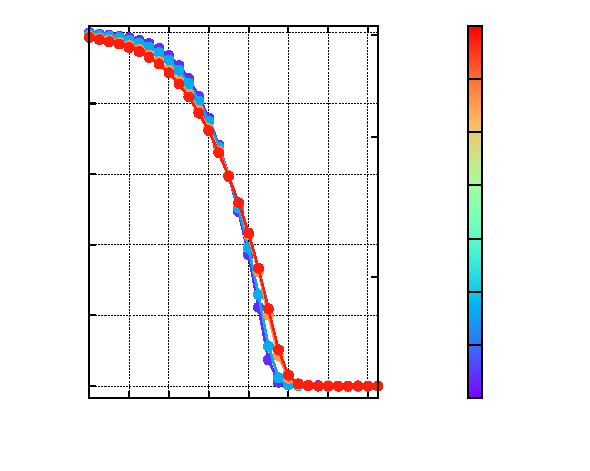
\includegraphics{LudoxHS40TransmissionCalibration}}%
    \gplfronttext
  \end{picture}%
\endgroup

		\caption{Concentration gradient of 12 nm silica particles (Ludox HS40, Sigma-Aldrich, Missouri, USA) mesaured at 8000 eV. The large size of the colloids provides a long diffusion time.}
		\label{fig:LudoxHS40TransmissionCalibration}
\end{figure}

The large difference in transmission for high-concentrated particles (7 to 1.2 is a ratio of ca. 6) is due to the high density of the sample 1.3 g cm-3

Possibility to make in-situ concentration series. and study the possible interaction between colloids depending on the interparticle distance or even study the crystallization of colloids\citep{hellsing_structure_2012}.

		
	\chapter{Simultaneous size and density determination of polymeric colloids}
\label{chap:simultaneous_size_density}
The current advances in nanomaterial development for medical applications are focused towards tailoring polymeric nano-drug carriers with flexible surface functionalisation and controlled morphologies \citep{euliss_imparting_2006,yang_shape-memory_2005}. Size and shape, combined with the choice of polymer and the mechanical properties, are fundamental and defining aspects of the particle functions, e.g. their \emph{in-vivo} biodistribution \citep{vittaz_effect_1996,mitragotri_physical_2009,doshi_designer_2009} or their drug-delivery efficacy \citep{powers_research_2006}. Therefore, a full and consistent characterization of all properties of nanoparticles is of crucial importance and must be carefully adressed, especially for polymeric NPs due to their typical complicate internal structure.

This chapter demonstrates the simultaneous size and density determination using continuous contrast variation technique in SAXS with 3 polymeric particles of different sizes and polymeric species. By means of an aqueous sucrose density gradient, the measurements were achieved along a large range of suspending medium densities, from water density to that of poly(methyl methacrylate)'s, highlighting the relevance of the technique across a wide spectrum of polymers.

The applicability of this method for the traceable size determination of these colloids is discussed in this chapter, where a high-resolution size distribution of the particles is presented. Focusing on a low-density colloid, different evaluation approaches to SAXS contrast variation experiments are discussed and the advantages and drawbacks of a model-free formulation like the isoscattering point position are discussed, together with the accuracy of the shape scattering function. In addition, a form factor model is fitted to the scattering curves to obtain decisive information about the internal morphology of the particle, which is not directly available by other techniques such as transmission scanning electron microscopy (TSEM), differential centrifugal sedimentation (DCS) \citep{fielding_correcting_2012} or atomic force microscopy (AFM). 

Besides, the ability of this technique to determine the density of polymeric colloids in suspension is also discussed. Normally, the density of the suspended particles can not be compared to the bulk density of the dry material. Such a complex question has been addressed by different methods, though with evident limitations. For example, the density of polymeric beads has been measured previously with field-flow fractionation (FFF) with high-accuracy but at the expense of \emph{a priori} assumptions about the morphology of the particle \citep{giddings_density_1981,yang_colloid_1983,caldwell_measurement_1986}. Assuming the Stokes' diameter as the actual size of the colloid, recent advances in analytical ultracentrifugation allow the complementary characterization of the size, density and molecular weight of gold nanoparticles \citep{carney_determination_2011}.

The density of the 3 polymeric colloids was also analysed by DCS and the results compared and discussed with those obtained by SAXS. DCS uses the sedimentation of particles through a density gradient to measure high resolution particle size distributions \citep{minelli_characterization_2014}. Its accuracy typically depends on the knowledge of the density of the particles. When the size of the particle is known, DCS can alternatively be used to measure average particle's density.

In this study, the size and density of low-density particles is independently determined by performing DCS measurements with two different discs using the sedimentation and flotation respectively of the particles through a density gradient and solving the relative Stokes' equations. A similar approach to DCS which combines the results of two independent measurements has been investigated previously. For example, \cite{neumann_new_2013} used two sucrose gradients resulting in different viscosities and densities, where the altered settling velocity combined with linear regression analysis was used for the calculation of the size and density of silica nanoparticles and viruses. \cite{bell_emerging_2012} adopted a two gradient method based on the variation of the sucrose concentration to determine the density of the St\"ober silica and the calibration standards used in DCS.

\section{Materials and methods}
In this section, a detailed description of the polymeric nanoparticles employed in the experiments is presented. The experimental procedure of the continuous contrast variation technique is thoroughly discussed already in chapter \ref{chap:density_gradient_SAXS}, thus the focus of the section lies only on the DCS technique. Special interest is put on the description of the combined DCS approach based on the floating-sedimentation principle.


\subsection{Polymeric particles}

The experiments were performed using 3 different types of polymeric nanoparticles, whose diameters range from 100 nm to around 187 nm. Carboxylated poly(methyl methacrylate) colloids (PMMA-COOH) with a nominal diameter of 187 nm and plain polystyrene particles (PS-Plain) polymerized with $<1$ wt$\%$ of a surface-active co-monomer with a nominal diameter of 147 nm were purchased from Microparticles (Berlin, Germany). The PS-COOH particles are described in detail in chapter \ref{chap:density_gradient_SAXS} and are composed of a PS core surrounded by a PMMA shell. The phyisical densities of the NPs range from that of PS (1.05 g cm$^{-3}$) until PMMA's, which has a density of ca. 1.18 g cm$^{-3}$.

For the preparation of the high density aqueous sucrose solutions employed in the density gradient capillaries, the suspended colloids were mixed with a sucrose mass fraction of 21.2 $\%$, 42.5 $\%$ and 13.4 $\%$ for the PS-COOH, PMMA-COOH and PS-Plain particles respectively.


\subsection{Differential Centrifugal Sedimentation}
\label{sec:DCS_experimental}
DCS measurements were performed in the National Physical Laboratory (NPL, Teddington, UK) with a CPS DC20000 instrument (CPS Instruments, Prairieville, LA, USA) upgraded to DC24000 for the PS-Plain particles measurements. The radial position of the detector was measured by injecting 100 $\mu$L aliquots of water into the spinning disc initially empty until the accumulation of water produced a response in the detector. For the density gradient formation, the disc was filled with 14.4 mL of a sucrose (Amresco LLC, OH, USA) solution topped with 0.5 mL of dodecane to prevent evaporation. The detailed information of the gradients is summarised in table \ref{tab:DCSParameters}. Measurements of the PS-COOH and PMMA-COOH particles at 0.05 \% w/v concentration were performed in triplicate. The measurements of the PS-Plain particles were repeated seven times for each setup. Injection volumes were 100 $\mu$L. 

\begin{table*}[]
\centering
\caption[Parameters of the different DCS setups.]{Parameters of the different DCS setups: composition of the sucrose gradients, average density of the gradients $\rho_f$, rotation speed of the centrifuge $\Omega$ and type of calibrant.}
\label{tab:DCSParameters}
\begin{tabular}{l|c|c|c|c|}
\cline{2-5}
\multicolumn{1}{c|}{}                         & Sucrose concentration (w/w)    & $\rho_f$ (g cm$^{-3}$) & $\Omega$ (rpm)  & Calibrant \\ \hline
\multicolumn{1}{|l|}{PS-COOH}    & from 2 \% to 8 \% in H$_2$0  & 1.013                  & 2.0$\cdot 10^4$                  & A         \\ \hline
\multicolumn{1}{|l|}{PMMA-COOH}  & from 4 \% to 12 \% in H$_2$0 & 1.025                  & 2.0$\cdot 10^4$                  & B         \\ \hline
\multicolumn{1}{|l|}{PS-Plain}      & from 2 \% to 8 \% in H$_2$0  & 1.013     & 2.4$\cdot 10^4$                  & B        \\ \hline
\multicolumn{1}{|l|}{PS-Plain*} & from 4 \% to 12 \% in D$_2$0 & 1.140     & 2.4$\cdot 10^4$                  & C         \\ \hline

\end{tabular}\\[0.3\baselineskip]
\begin{minipage}{15cm}
	\begin{raggedright}
	*\small{Low density disc}
	\end{raggedright}
\end{minipage}
\label{tab:composition}
\end{table*}

The measured attenuation at 405 nm was converted to the number of particles for each measured diameter by treating the particles as spherical Mie scatterers with no optical absorbance at the incident wavelength. Three different types of calibration particles were used: poly(vinyl chloride) colloids in water with density of 1.385 g cm$^{-3}$ and nominal size of $(223\pm5)$ nm (calibrant A) and $(239\pm5)$ nm (calibrant B) and polybutadiene colloids in 16 \% sucrose mass fraction in heavy water with nominal size of $(510\pm20)$ nm and density of 0.91 g cm$^{-3}$ (calibrant C). 

A standard disc configuration where the particles sediment through a lower density gradient was used and additionally, a more recently developed set up which makes use of a disc where colloids float through a higher density gradient was also used for the PS-Plain colloids due to their low density \citep{fitzpatrick_structure_1998}. Typically, the DCS diameter $D_p$ or density $\rho_p$ of a spherical particle is derived from the Stokes' law:

\begin{equation}
D_p=\sqrt{\frac{18\eta\ln\sfrac{R_f}{R_i}}{\left( \rho_p - \rho_{\text{fluid}} \right)\omega^2 t_p}}
\label{eq:stokes}
\end{equation}

where $t_p$ is the sedimentation time between radii of rotation $R_f$ and $R_i$ of the particle, $\eta$ and $\rho_f$ are the viscosity and the density of the fluid respectively and $\omega$ is the disc angular frequency. If a calibrant of known diameter $D_c$ and density $\rho_c$ is measured with the same set up, the investigated particle diameter can be expressed as:

\begin{equation}
D_p=D_c\sqrt{\frac{\left( \rho_c - \rho_{\text{fluid}} \right) t_c}{\left( \rho_p - \rho_{\text{fluid}} \right) t_p}}
\label{eq:software}
\end{equation}

By using the combination of DCS measurements performed in two different fluids, one with density $\rho_L$ and one with higher density $\rho_H$, the values of $D_p$ and $\rho_p$ can be independently found by solving analytically the following system of equations:

\begin{equation}
\bm{D_p} = D_{cH}\sqrt{\frac{\left( \rho_{cH} - \rho_H \right) t_{cH}}{\left( \bm{\rho_p} - \rho_H \right) t_{pH}}} = D_{cL}\sqrt{\frac{\left( \rho_{cL} - \rho_L \right) t_{cL}}{\left( \bm{\rho_p} - \rho_L \right) t_{pL}}}
\label{eq:DCS_sys}
\end{equation}

where $cH$ and $cL$ denote the calibrants used with high and low density fluids respectively and $t_{pH}$ and $t_{pL}$ are the sedimentation times of the particles measured in the high and low density fluids respectively. The measurement uncertanties given in the text include both statistical and systematic uncertainty propagated from Stokes' equations.

\section{Determination of the particle size distribution}
\label{sec:size_validation}

\begin{figure}
	\begin{center}
		% GNUPLOT: LaTeX picture with Postscript
\begingroup
  \makeatletter
  \providecommand\color[2][]{%
    \GenericError{(gnuplot) \space\space\space\@spaces}{%
      Package color not loaded in conjunction with
      terminal option `colourtext'%
    }{See the gnuplot documentation for explanation.%
    }{Either use 'blacktext' in gnuplot or load the package
      color.sty in LaTeX.}%
    \renewcommand\color[2][]{}%
  }%
  \providecommand\includegraphics[2][]{%
    \GenericError{(gnuplot) \space\space\space\@spaces}{%
      Package graphicx or graphics not loaded%
    }{See the gnuplot documentation for explanation.%
    }{The gnuplot epslatex terminal needs graphicx.sty or graphics.sty.}%
    \renewcommand\includegraphics[2][]{}%
  }%
  \providecommand\rotatebox[2]{#2}%
  \@ifundefined{ifGPcolor}{%
    \newif\ifGPcolor
    \GPcolortrue
  }{}%
  \@ifundefined{ifGPblacktext}{%
    \newif\ifGPblacktext
    \GPblacktextfalse
  }{}%
  % define a \g@addto@macro without @ in the name:
  \let\gplgaddtomacro\g@addto@macro
  % define empty templates for all commands taking text:
  \gdef\gplbacktext{}%
  \gdef\gplfronttext{}%
  \makeatother
  \ifGPblacktext
    % no textcolor at all
    \def\colorrgb#1{}%
    \def\colorgray#1{}%
  \else
    % gray or color?
    \ifGPcolor
      \def\colorrgb#1{\color[rgb]{#1}}%
      \def\colorgray#1{\color[gray]{#1}}%
      \expandafter\def\csname LTw\endcsname{\color{white}}%
      \expandafter\def\csname LTb\endcsname{\color{black}}%
      \expandafter\def\csname LTa\endcsname{\color{black}}%
      \expandafter\def\csname LT0\endcsname{\color[rgb]{1,0,0}}%
      \expandafter\def\csname LT1\endcsname{\color[rgb]{0,1,0}}%
      \expandafter\def\csname LT2\endcsname{\color[rgb]{0,0,1}}%
      \expandafter\def\csname LT3\endcsname{\color[rgb]{1,0,1}}%
      \expandafter\def\csname LT4\endcsname{\color[rgb]{0,1,1}}%
      \expandafter\def\csname LT5\endcsname{\color[rgb]{1,1,0}}%
      \expandafter\def\csname LT6\endcsname{\color[rgb]{0,0,0}}%
      \expandafter\def\csname LT7\endcsname{\color[rgb]{1,0.3,0}}%
      \expandafter\def\csname LT8\endcsname{\color[rgb]{0.5,0.5,0.5}}%
    \else
      % gray
      \def\colorrgb#1{\color{black}}%
      \def\colorgray#1{\color[gray]{#1}}%
      \expandafter\def\csname LTw\endcsname{\color{white}}%
      \expandafter\def\csname LTb\endcsname{\color{black}}%
      \expandafter\def\csname LTa\endcsname{\color{black}}%
      \expandafter\def\csname LT0\endcsname{\color{black}}%
      \expandafter\def\csname LT1\endcsname{\color{black}}%
      \expandafter\def\csname LT2\endcsname{\color{black}}%
      \expandafter\def\csname LT3\endcsname{\color{black}}%
      \expandafter\def\csname LT4\endcsname{\color{black}}%
      \expandafter\def\csname LT5\endcsname{\color{black}}%
      \expandafter\def\csname LT6\endcsname{\color{black}}%
      \expandafter\def\csname LT7\endcsname{\color{black}}%
      \expandafter\def\csname LT8\endcsname{\color{black}}%
    \fi
  \fi
  \setlength{\unitlength}{0.0500bp}%
  \begin{picture}(5668.00,4534.00)%
    \gplgaddtomacro\gplbacktext{%
      \csname LTb\endcsname%
      \put(990,704){\makebox(0,0)[r]{\strut{} 0.1}}%
      \csname LTb\endcsname%
      \put(990,1355){\makebox(0,0)[r]{\strut{} 1}}%
      \csname LTb\endcsname%
      \put(990,2006){\makebox(0,0)[r]{\strut{} 10}}%
      \csname LTb\endcsname%
      \put(990,2657){\makebox(0,0)[r]{\strut{} 100}}%
      \csname LTb\endcsname%
      \put(990,3308){\makebox(0,0)[r]{\strut{} 1000}}%
      \csname LTb\endcsname%
      \put(990,3958){\makebox(0,0)[r]{\strut{} 10000}}%
      \csname LTb\endcsname%
      \put(1122,484){\makebox(0,0){\strut{} 0.02}}%
      \csname LTb\endcsname%
      \put(1586,484){\makebox(0,0){\strut{} 0.03}}%
      \csname LTb\endcsname%
      \put(2171,484){\makebox(0,0){\strut{} 0.05}}%
      \csname LTb\endcsname%
      \put(2964,484){\makebox(0,0){\strut{} 0.1}}%
      \csname LTb\endcsname%
      \put(3758,484){\makebox(0,0){\strut{} 0.2}}%
      \csname LTb\endcsname%
      \put(4222,484){\makebox(0,0){\strut{} 0.3}}%
      \csname LTb\endcsname%
      \put(4807,484){\makebox(0,0){\strut{} 0.5}}%
      \put(220,2486){\rotatebox{-270}{\makebox(0,0){\strut{}Scattering Intensity / a.u.}}}%
      \put(3196,154){\makebox(0,0){\strut{}$q$ / nm$^{-1}$}}%
    }%
    \gplgaddtomacro\gplfronttext{%
      \csname LTb\endcsname%
      \put(3063,1386){\makebox(0,0)[r]{\strut{}PS-Plain in buffer}}%
      \csname LTb\endcsname%
      \put(3063,1056){\makebox(0,0)[r]{\strut{}Core-Shell Fit}}%
    }%
    \gplgaddtomacro\gplbacktext{%
      \csname LTb\endcsname%
      \put(3862,3016){\makebox(0,0)[r]{\strut{}\footnotesize 333}}%
      \csname LTb\endcsname%
      \put(3862,3278){\makebox(0,0)[r]{\strut{}\footnotesize 337}}%
      \csname LTb\endcsname%
      \put(3862,3539){\makebox(0,0)[r]{\strut{}\footnotesize 341}}%
      \csname LTb\endcsname%
      \put(3862,3801){\makebox(0,0)[r]{\strut{}\footnotesize 345}}%
      \csname LTb\endcsname%
      \put(3994,2796){\makebox(0,0){\strut{}\footnotesize 0}}%
      \csname LTb\endcsname%
      \put(4367,2796){\makebox(0,0){\strut{}\footnotesize 25}}%
      \csname LTb\endcsname%
      \put(4740,2796){\makebox(0,0){\strut{}\footnotesize 50}}%
      \csname LTb\endcsname%
      \put(5112,2796){\makebox(0,0){\strut{}\footnotesize 75}}%
      \put(3356,3572){\rotatebox{-270}{\makebox(0,0){\strut{}\footnotesize{$\rho_e$ / nm$^{-3}$}}}}%
      \put(4575,2466){\makebox(0,0){\strut{}\footnotesize{$R$} / nm}}%
    }%
    \gplgaddtomacro\gplfronttext{%
    }%
    \gplbacktext
    \put(0,0){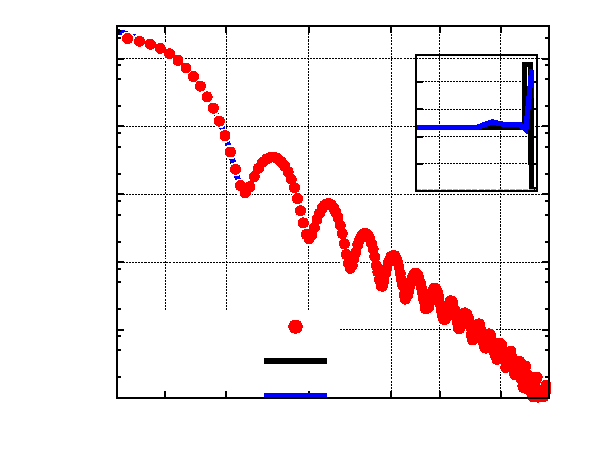
\includegraphics{PSPlainSingleContrastSAXS}}%
    \gplfronttext
  \end{picture}%
\endgroup

	\end{center}
	\caption[Scattering curve of the PS-Plain particles in buffer.]{Scattering curve of the PS-Plain particles in buffer: A core–shell fit to the experimental scattering curve is presented. In the inset, the electron density radial profile of this fit is shown, assuming the core is polystyrene with a density of 339.7 nm$^{-3}$.}
	\label{fig:PSPlainSingleContrastSAXS}
\end{figure}

In figure \ref{fig:PSPlainSingleContrastSAXS}, the SAXS curve of the PS-Plain particles in buffer at a single-contrast is shown. The large number of minima observed in the curve is remarkable and indicates the high monodispersity of the sample, which allows a traceable size determination of these colloids.

Upon trying different form factor fits detailed in section \ref{sec:SAXS_theory}, a simple core-shell structure with a sharp interface (eq. \ref{eq:ff_cs}) was found to be the most suitable, suggesting a heterogeneous structure which is eluded by other characterization techniques, e.g. microscopy. The obtained particle diameter was $(147.0\pm4.7)$ nm, where the fit uncertainty was calculated with a confidence level of one standard deviation ($k=1$) by examining the change in $\chi^2$ when varying the diameter. The radial electron density profile of the core-shell fit is shown in the inset of figure \ref{fig:PSPlainSingleContrastSAXS}, where a thin shell with high density surrounds a lighter core. This structure is likely due to the non-reacted monomers in the main matrix or the highly hydrophilic behaviour of the co-monomer, segregating polystyrene to the core.

The fit of the form factor \ref{eq:multicore-shell} with 7 shells with a linear electron density gradient is in very good agreement with the experimental data as well and presents a $\chi^2$ value 20 times lower than the compact spheres model fit. Although the radial electron density profile coincides qualitatively with the core-shell model, the result might not be unique due to the large number of fiting parameters (14) and care must be taken.

The morphology of the PS-Plain particles was further studied using the density gradient contrast variation technique described in chapter \ref{chap:density_gradient_SAXS} by varying the suspending medium electron density from 333.2 to 350.2 nm$^{-3}$. By increasing the solvent contrast, the changes of the features in the scattering curves presented in figure \ref{fig:PSPlainContinuousSAXS} and the appearance of isoscattering points prove the multi-component composition of this colloid.

\begin{figure*}%[htbp]
	\centering
                \subfloat[Scattering curves]{\resizebox{0.44\linewidth}{!}{\figfont{13pt}% GNUPLOT: LaTeX picture with Postscript
\begingroup
  \makeatletter
  \providecommand\color[2][]{%
    \GenericError{(gnuplot) \space\space\space\@spaces}{%
      Package color not loaded in conjunction with
      terminal option `colourtext'%
    }{See the gnuplot documentation for explanation.%
    }{Either use 'blacktext' in gnuplot or load the package
      color.sty in LaTeX.}%
    \renewcommand\color[2][]{}%
  }%
  \providecommand\includegraphics[2][]{%
    \GenericError{(gnuplot) \space\space\space\@spaces}{%
      Package graphicx or graphics not loaded%
    }{See the gnuplot documentation for explanation.%
    }{The gnuplot epslatex terminal needs graphicx.sty or graphics.sty.}%
    \renewcommand\includegraphics[2][]{}%
  }%
  \providecommand\rotatebox[2]{#2}%
  \@ifundefined{ifGPcolor}{%
    \newif\ifGPcolor
    \GPcolortrue
  }{}%
  \@ifundefined{ifGPblacktext}{%
    \newif\ifGPblacktext
    \GPblacktextfalse
  }{}%
  % define a \g@addto@macro without @ in the name:
  \let\gplgaddtomacro\g@addto@macro
  % define empty templates for all commands taking text:
  \gdef\gplbacktext{}%
  \gdef\gplfronttext{}%
  \makeatother
  \ifGPblacktext
    % no textcolor at all
    \def\colorrgb#1{}%
    \def\colorgray#1{}%
  \else
    % gray or color?
    \ifGPcolor
      \def\colorrgb#1{\color[rgb]{#1}}%
      \def\colorgray#1{\color[gray]{#1}}%
      \expandafter\def\csname LTw\endcsname{\color{white}}%
      \expandafter\def\csname LTb\endcsname{\color{black}}%
      \expandafter\def\csname LTa\endcsname{\color{black}}%
      \expandafter\def\csname LT0\endcsname{\color[rgb]{1,0,0}}%
      \expandafter\def\csname LT1\endcsname{\color[rgb]{0,1,0}}%
      \expandafter\def\csname LT2\endcsname{\color[rgb]{0,0,1}}%
      \expandafter\def\csname LT3\endcsname{\color[rgb]{1,0,1}}%
      \expandafter\def\csname LT4\endcsname{\color[rgb]{0,1,1}}%
      \expandafter\def\csname LT5\endcsname{\color[rgb]{1,1,0}}%
      \expandafter\def\csname LT6\endcsname{\color[rgb]{0,0,0}}%
      \expandafter\def\csname LT7\endcsname{\color[rgb]{1,0.3,0}}%
      \expandafter\def\csname LT8\endcsname{\color[rgb]{0.5,0.5,0.5}}%
    \else
      % gray
      \def\colorrgb#1{\color{black}}%
      \def\colorgray#1{\color[gray]{#1}}%
      \expandafter\def\csname LTw\endcsname{\color{white}}%
      \expandafter\def\csname LTb\endcsname{\color{black}}%
      \expandafter\def\csname LTa\endcsname{\color{black}}%
      \expandafter\def\csname LT0\endcsname{\color{black}}%
      \expandafter\def\csname LT1\endcsname{\color{black}}%
      \expandafter\def\csname LT2\endcsname{\color{black}}%
      \expandafter\def\csname LT3\endcsname{\color{black}}%
      \expandafter\def\csname LT4\endcsname{\color{black}}%
      \expandafter\def\csname LT5\endcsname{\color{black}}%
      \expandafter\def\csname LT6\endcsname{\color{black}}%
      \expandafter\def\csname LT7\endcsname{\color{black}}%
      \expandafter\def\csname LT8\endcsname{\color{black}}%
    \fi
  \fi
  \setlength{\unitlength}{0.0500bp}%
  \begin{picture}(5668.00,4534.00)%
    \gplgaddtomacro\gplbacktext{%
      \csname LTb\endcsname%
      \put(858,1156){\makebox(0,0)[r]{\strut{} 1}}%
      \csname LTb\endcsname%
      \put(858,2020){\makebox(0,0)[r]{\strut{} 10}}%
      \csname LTb\endcsname%
      \put(858,2884){\makebox(0,0)[r]{\strut{} 100}}%
      \csname LTb\endcsname%
      \put(858,3749){\makebox(0,0)[r]{\strut{} 1000}}%
      \csname LTb\endcsname%
      \put(1287,484){\makebox(0,0){\strut{} 0.03}}%
      \csname LTb\endcsname%
      \put(1858,484){\makebox(0,0){\strut{} 0.05}}%
      \csname LTb\endcsname%
      \put(2633,484){\makebox(0,0){\strut{} 0.1}}%
      \csname LTb\endcsname%
      \put(3408,484){\makebox(0,0){\strut{} 0.2}}%
      \csname LTb\endcsname%
      \put(3862,484){\makebox(0,0){\strut{} 0.3}}%
      \csname LTb\endcsname%
      \put(4433,484){\makebox(0,0){\strut{} 0.5}}%
      \put(220,2266){\rotatebox{-270}{\makebox(0,0){\strut{}Scattering Intensity / a.u.}}}%
      \put(2711,154){\makebox(0,0){\strut{}$q$ / nm$^{-1}$}}%
    }%
    \gplgaddtomacro\gplfronttext{%
      \csname LTb\endcsname%
      \put(4692,704){\makebox(0,0)[l]{\strut{}\fsmedium 334}}%
      \put(4692,1213){\makebox(0,0)[l]{\strut{}\fsmedium 336}}%
      \put(4692,1722){\makebox(0,0)[l]{\strut{}\fsmedium 338}}%
      \put(4692,2231){\makebox(0,0)[l]{\strut{}\fsmedium 340}}%
      \put(4692,2741){\makebox(0,0)[l]{\strut{}\fsmedium 342}}%
      \put(4692,3250){\makebox(0,0)[l]{\strut{}\fsmedium 344}}%
      \put(4692,3759){\makebox(0,0)[l]{\strut{}\fsmedium 346}}%
      \put(4692,4269){\makebox(0,0)[l]{\strut{}\fsmedium 348}}%
      \put(5418,2486){\rotatebox{-90}{\makebox(0,0){\strut{}\fsmedium Solvent Electron Density / nm$^{-3}$}}}%
    }%
    \gplbacktext
    \put(0,0){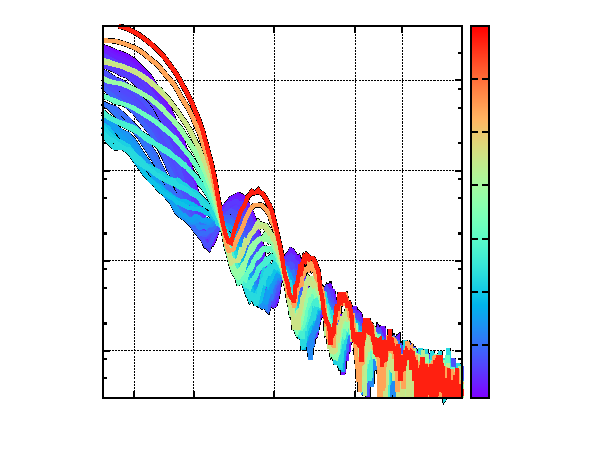
\includegraphics{PSPlainContinuousSAXS}}%
    \gplfronttext
  \end{picture}%
\endgroup
}\label{fig:PSPlainContinuousSAXS}}
		\subfloat[Isoscattering point positions]{\resizebox{0.44\linewidth}{!}{\figfont{13pt}% GNUPLOT: LaTeX picture with Postscript
\begingroup
  \makeatletter
  \providecommand\color[2][]{%
    \GenericError{(gnuplot) \space\space\space\@spaces}{%
      Package color not loaded in conjunction with
      terminal option `colourtext'%
    }{See the gnuplot documentation for explanation.%
    }{Either use 'blacktext' in gnuplot or load the package
      color.sty in LaTeX.}%
    \renewcommand\color[2][]{}%
  }%
  \providecommand\includegraphics[2][]{%
    \GenericError{(gnuplot) \space\space\space\@spaces}{%
      Package graphicx or graphics not loaded%
    }{See the gnuplot documentation for explanation.%
    }{The gnuplot epslatex terminal needs graphicx.sty or graphics.sty.}%
    \renewcommand\includegraphics[2][]{}%
  }%
  \providecommand\rotatebox[2]{#2}%
  \@ifundefined{ifGPcolor}{%
    \newif\ifGPcolor
    \GPcolortrue
  }{}%
  \@ifundefined{ifGPblacktext}{%
    \newif\ifGPblacktext
    \GPblacktextfalse
  }{}%
  % define a \g@addto@macro without @ in the name:
  \let\gplgaddtomacro\g@addto@macro
  % define empty templates for all commands taking text:
  \gdef\gplbacktext{}%
  \gdef\gplfronttext{}%
  \makeatother
  \ifGPblacktext
    % no textcolor at all
    \def\colorrgb#1{}%
    \def\colorgray#1{}%
  \else
    % gray or color?
    \ifGPcolor
      \def\colorrgb#1{\color[rgb]{#1}}%
      \def\colorgray#1{\color[gray]{#1}}%
      \expandafter\def\csname LTw\endcsname{\color{white}}%
      \expandafter\def\csname LTb\endcsname{\color{black}}%
      \expandafter\def\csname LTa\endcsname{\color{black}}%
      \expandafter\def\csname LT0\endcsname{\color[rgb]{1,0,0}}%
      \expandafter\def\csname LT1\endcsname{\color[rgb]{0,1,0}}%
      \expandafter\def\csname LT2\endcsname{\color[rgb]{0,0,1}}%
      \expandafter\def\csname LT3\endcsname{\color[rgb]{1,0,1}}%
      \expandafter\def\csname LT4\endcsname{\color[rgb]{0,1,1}}%
      \expandafter\def\csname LT5\endcsname{\color[rgb]{1,1,0}}%
      \expandafter\def\csname LT6\endcsname{\color[rgb]{0,0,0}}%
      \expandafter\def\csname LT7\endcsname{\color[rgb]{1,0.3,0}}%
      \expandafter\def\csname LT8\endcsname{\color[rgb]{0.5,0.5,0.5}}%
    \else
      % gray
      \def\colorrgb#1{\color{black}}%
      \def\colorgray#1{\color[gray]{#1}}%
      \expandafter\def\csname LTw\endcsname{\color{white}}%
      \expandafter\def\csname LTb\endcsname{\color{black}}%
      \expandafter\def\csname LTa\endcsname{\color{black}}%
      \expandafter\def\csname LT0\endcsname{\color{black}}%
      \expandafter\def\csname LT1\endcsname{\color{black}}%
      \expandafter\def\csname LT2\endcsname{\color{black}}%
      \expandafter\def\csname LT3\endcsname{\color{black}}%
      \expandafter\def\csname LT4\endcsname{\color{black}}%
      \expandafter\def\csname LT5\endcsname{\color{black}}%
      \expandafter\def\csname LT6\endcsname{\color{black}}%
      \expandafter\def\csname LT7\endcsname{\color{black}}%
      \expandafter\def\csname LT8\endcsname{\color{black}}%
    \fi
  \fi
  \setlength{\unitlength}{0.0500bp}%
  \begin{picture}(5668.00,4534.00)%
    \gplgaddtomacro\gplbacktext{%
      \csname LTb\endcsname%
      \put(858,682){\makebox(0,0)[r]{\strut{} 0.02}}%
      \csname LTb\endcsname%
      \put(858,1493){\makebox(0,0)[r]{\strut{} 0.05}}%
      \csname LTb\endcsname%
      \put(858,2107){\makebox(0,0)[r]{\strut{} 0.1}}%
      \csname LTb\endcsname%
      \put(858,2720){\makebox(0,0)[r]{\strut{} 0.2}}%
      \csname LTb\endcsname%
      \put(858,3532){\makebox(0,0)[r]{\strut{} 0.5}}%
      \csname LTb\endcsname%
      \put(858,4145){\makebox(0,0)[r]{\strut{} 1}}%
      \csname LTb\endcsname%
      \put(990,462){\makebox(0,0){\strut{} 0.05}}%
      \csname LTb\endcsname%
      \put(2834,462){\makebox(0,0){\strut{} 0.1}}%
      \csname LTb\endcsname%
      \put(4677,462){\makebox(0,0){\strut{} 0.2}}%
      \put(180,2475){\rotatebox{-270}{\makebox(0,0){\strut{}Rel. Std. Deviation}}}%
      \put(3130,154){\makebox(0,0){\strut{}$q$ / nm$^{-1}$}}%
      \put(1339,1909){\makebox(0,0)[l]{\strut{}$I_1$}}%
      \put(2766,1725){\makebox(0,0)[l]{\strut{}$I_2$}}%
      \put(3632,1655){\makebox(0,0)[l]{\strut{}$I_3$}}%
      \put(4325,1963){\makebox(0,0)[l]{\strut{}$I_4$}}%
      \put(4888,1909){\makebox(0,0)[l]{\strut{}$I_5$}}%
    }%
    \gplgaddtomacro\gplfronttext{%
      \csname LTb\endcsname%
      \put(4548,4041){\makebox(0,0)[r]{\strut{}\smaller Background subtracted}}%
      \csname LTb\endcsname%
      \put(4548,3711){\makebox(0,0)[r]{\strut{}\smaller Raw data}}%
    }%
    \gplbacktext
    \put(0,0){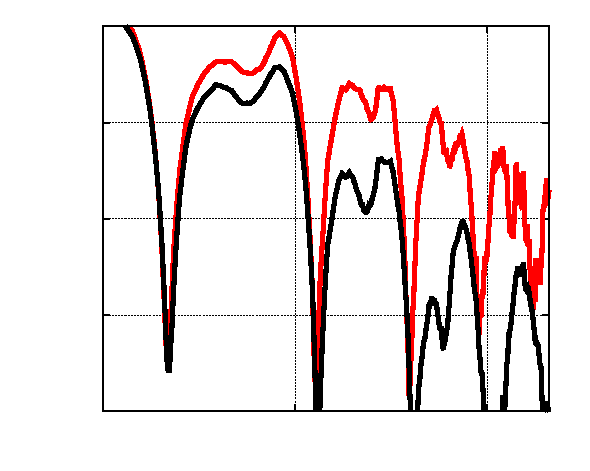
\includegraphics{PSPlainContinuousSAXSIsopoint}}%
    \gplfronttext
  \end{picture}%
\endgroup
}\label{fig:PSPlainContinuousSAXSIsopoint}}
	\caption[Continuous contrast variation experimental data of the PS-Plain particles.]{Continuous contrast variation on the PS-Plain particles: a) SAXS curves of the PS-Plain particles obtained by density gradient contrast variation after solvent background subtraction. b) The relative standard deviation of each $q$ calculated across all the measured scattering curves, where the minima correspond to the isoscattering points $I_i$. The background subtraction shifts the position of $I_i$, especially for high $q$-values.}
\end{figure*}

From the 40 experimental scattering curves shown in figure \ref{fig:PSPlainContinuousSAXS}, a model-free size determination can be performed by locating the isoscattering points $I_i$. This is achieved by calculating the relative standard deviation, as shown in figure \ref{fig:PSPlainContinuousSAXSIsopoint}, where the minima correspond to the fulfillment of the isoscattering condition expressed by equation \ref{eq:isoscattering}.

The particle diameters obtained from the first 4 isoscattering points ($I_1$ to $I_4$) range between 142.4 and 144.4 nm, showing a good agreement for higher $q$-values as well. The precision of the isoscattering point determination decreases for increasing $q$ as demonstrated by \cite{kawaguchi_isoscattering_1992} and it is exemplified by the broadening of the minima for higher $q$. As observed in figure \ref{fig:PSPlainContinuousSAXSIsopoint}, the effect of the solvent background is relevant principally at high $q$-values as well.

The data can also be analysed by using the \emph{shape scattering function} described in section \ref{sec:basic_functions_theory}. The shape scattering function describes the external shape of the particle independently of its inner structure and is an appropriate approach for the PS-Plain colloid, because it enables the size distribution determination of the particles avoiding any \emph{a priori} consideration about the particle composition.

\begin{figure}
	\begin{center}
		% GNUPLOT: LaTeX picture with Postscript
\begingroup
  \makeatletter
  \providecommand\color[2][]{%
    \GenericError{(gnuplot) \space\space\space\@spaces}{%
      Package color not loaded in conjunction with
      terminal option `colourtext'%
    }{See the gnuplot documentation for explanation.%
    }{Either use 'blacktext' in gnuplot or load the package
      color.sty in LaTeX.}%
    \renewcommand\color[2][]{}%
  }%
  \providecommand\includegraphics[2][]{%
    \GenericError{(gnuplot) \space\space\space\@spaces}{%
      Package graphicx or graphics not loaded%
    }{See the gnuplot documentation for explanation.%
    }{The gnuplot epslatex terminal needs graphicx.sty or graphics.sty.}%
    \renewcommand\includegraphics[2][]{}%
  }%
  \providecommand\rotatebox[2]{#2}%
  \@ifundefined{ifGPcolor}{%
    \newif\ifGPcolor
    \GPcolortrue
  }{}%
  \@ifundefined{ifGPblacktext}{%
    \newif\ifGPblacktext
    \GPblacktextfalse
  }{}%
  % define a \g@addto@macro without @ in the name:
  \let\gplgaddtomacro\g@addto@macro
  % define empty templates for all commands taking text:
  \gdef\gplbacktext{}%
  \gdef\gplfronttext{}%
  \makeatother
  \ifGPblacktext
    % no textcolor at all
    \def\colorrgb#1{}%
    \def\colorgray#1{}%
  \else
    % gray or color?
    \ifGPcolor
      \def\colorrgb#1{\color[rgb]{#1}}%
      \def\colorgray#1{\color[gray]{#1}}%
      \expandafter\def\csname LTw\endcsname{\color{white}}%
      \expandafter\def\csname LTb\endcsname{\color{black}}%
      \expandafter\def\csname LTa\endcsname{\color{black}}%
      \expandafter\def\csname LT0\endcsname{\color[rgb]{1,0,0}}%
      \expandafter\def\csname LT1\endcsname{\color[rgb]{0,1,0}}%
      \expandafter\def\csname LT2\endcsname{\color[rgb]{0,0,1}}%
      \expandafter\def\csname LT3\endcsname{\color[rgb]{1,0,1}}%
      \expandafter\def\csname LT4\endcsname{\color[rgb]{0,1,1}}%
      \expandafter\def\csname LT5\endcsname{\color[rgb]{1,1,0}}%
      \expandafter\def\csname LT6\endcsname{\color[rgb]{0,0,0}}%
      \expandafter\def\csname LT7\endcsname{\color[rgb]{1,0.3,0}}%
      \expandafter\def\csname LT8\endcsname{\color[rgb]{0.5,0.5,0.5}}%
    \else
      % gray
      \def\colorrgb#1{\color{black}}%
      \def\colorgray#1{\color[gray]{#1}}%
      \expandafter\def\csname LTw\endcsname{\color{white}}%
      \expandafter\def\csname LTb\endcsname{\color{black}}%
      \expandafter\def\csname LTa\endcsname{\color{black}}%
      \expandafter\def\csname LT0\endcsname{\color{black}}%
      \expandafter\def\csname LT1\endcsname{\color{black}}%
      \expandafter\def\csname LT2\endcsname{\color{black}}%
      \expandafter\def\csname LT3\endcsname{\color{black}}%
      \expandafter\def\csname LT4\endcsname{\color{black}}%
      \expandafter\def\csname LT5\endcsname{\color{black}}%
      \expandafter\def\csname LT6\endcsname{\color{black}}%
      \expandafter\def\csname LT7\endcsname{\color{black}}%
      \expandafter\def\csname LT8\endcsname{\color{black}}%
    \fi
  \fi
    \setlength{\unitlength}{0.0500bp}%
    \ifx\gptboxheight\undefined%
      \newlength{\gptboxheight}%
      \newlength{\gptboxwidth}%
      \newsavebox{\gptboxtext}%
    \fi%
    \setlength{\fboxrule}{0.5pt}%
    \setlength{\fboxsep}{1pt}%
\begin{picture}(5668.00,4534.00)%
    \gplgaddtomacro\gplbacktext{%
      \csname LTb\endcsname%
      \put(990,704){\makebox(0,0)[r]{\strut{}$1$}}%
      \csname LTb\endcsname%
      \put(990,1377){\makebox(0,0)[r]{\strut{}$10$}}%
      \csname LTb\endcsname%
      \put(990,2049){\makebox(0,0)[r]{\strut{}$100$}}%
      \csname LTb\endcsname%
      \put(990,2722){\makebox(0,0)[r]{\strut{}$1000$}}%
      \csname LTb\endcsname%
      \put(990,3394){\makebox(0,0)[r]{\strut{}$10000$}}%
      \csname LTb\endcsname%
      \put(990,4067){\makebox(0,0)[r]{\strut{}$100000$}}%
      \csname LTb\endcsname%
      \put(1395,484){\makebox(0,0){\strut{}$0.03$}}%
      \csname LTb\endcsname%
      \put(2159,484){\makebox(0,0){\strut{}$0.05$}}%
      \csname LTb\endcsname%
      \put(3197,484){\makebox(0,0){\strut{}$0.1$}}%
      \csname LTb\endcsname%
      \put(4234,484){\makebox(0,0){\strut{}$0.2$}}%
      \csname LTb\endcsname%
      \put(4841,484){\makebox(0,0){\strut{}$0.3$}}%
    }%
    \gplgaddtomacro\gplfronttext{%
      \csname LTb\endcsname%
      \put(220,2486){\rotatebox{-270}{\makebox(0,0){\strut{}Scattering Intensity / a.u.}}}%
      \put(3196,154){\makebox(0,0){\strut{}$q$ / nm$^{-1}$}}%
      \csname LTb\endcsname%
      \put(4548,4041){\makebox(0,0)[r]{\strut{}\smaller Shape scattering function}}%
      \csname LTb\endcsname%
      \put(4548,3711){\makebox(0,0)[r]{\strut{}\smaller Spherical model}}%
    }%
    \gplbacktext
    \put(0,0){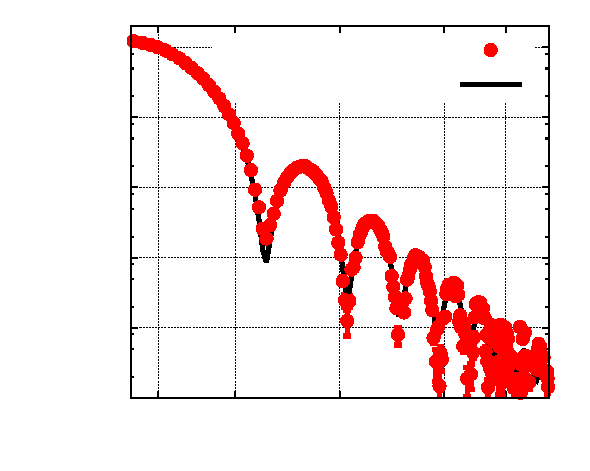
\includegraphics{PSPlainResonantTerm}}%
    \gplfronttext
  \end{picture}%
\endgroup

	\end{center}
	\caption[Experimental shape scattering function of the PS-Plain particles.]{Experimental shape scattering function of the PS-Plain particles calculated from 40 scattering curves and the spherical form factor fitted to the data.}
	\label{fig:PSPlainResonantTerm}
\end{figure}

The shape scattering function calculated from the measured scattering curves is depicted in figure \ref{fig:PSPlainResonantTerm} together with the spherical model fitted to the data, which employs a simple form factor that ignores the internal structure (eq. \ref{eq:ff_sphere}) and a gaussian size distribution expressed by equation \ref{eq:gauss_distribution}. From this fit, a mean particle size of $(146.8\pm1.3)$ nm was determined. The associated uncertainty calculated with this approach is 3.5 times smaller than the one obtained with the single-contrast SAXS experiment. By fitting the ellipsoid model given by expression \ref{eq:ff_ellipsoid} to the shape scattering function, a sphericity of 98 $\%$ was obtained.

\subsection{Inter-laboratory comparison of the mean particle diameter}
\label{sec:interlab_size_comparison}
The improvement in the size accuracy with the shape scattering function approach is summarized in figure \ref{fig:PSPlainSizeComparison}, where the diameter of the PS-Plain particles determined by different techniques in an inter-laboratory study is also presented \citep{nicolet_inter-laboratory_2016}.

\begin{figure*}
	\centering
		% GNUPLOT: LaTeX picture with Postscript
\begingroup
  \makeatletter
  \providecommand\color[2][]{%
    \GenericError{(gnuplot) \space\space\space\@spaces}{%
      Package color not loaded in conjunction with
      terminal option `colourtext'%
    }{See the gnuplot documentation for explanation.%
    }{Either use 'blacktext' in gnuplot or load the package
      color.sty in LaTeX.}%
    \renewcommand\color[2][]{}%
  }%
  \providecommand\includegraphics[2][]{%
    \GenericError{(gnuplot) \space\space\space\@spaces}{%
      Package graphicx or graphics not loaded%
    }{See the gnuplot documentation for explanation.%
    }{The gnuplot epslatex terminal needs graphicx.sty or graphics.sty.}%
    \renewcommand\includegraphics[2][]{}%
  }%
  \providecommand\rotatebox[2]{#2}%
  \@ifundefined{ifGPcolor}{%
    \newif\ifGPcolor
    \GPcolortrue
  }{}%
  \@ifundefined{ifGPblacktext}{%
    \newif\ifGPblacktext
    \GPblacktextfalse
  }{}%
  % define a \g@addto@macro without @ in the name:
  \let\gplgaddtomacro\g@addto@macro
  % define empty templates for all commands taking text:
  \gdef\gplbacktext{}%
  \gdef\gplfronttext{}%
  \makeatother
  \ifGPblacktext
    % no textcolor at all
    \def\colorrgb#1{}%
    \def\colorgray#1{}%
  \else
    % gray or color?
    \ifGPcolor
      \def\colorrgb#1{\color[rgb]{#1}}%
      \def\colorgray#1{\color[gray]{#1}}%
      \expandafter\def\csname LTw\endcsname{\color{white}}%
      \expandafter\def\csname LTb\endcsname{\color{black}}%
      \expandafter\def\csname LTa\endcsname{\color{black}}%
      \expandafter\def\csname LT0\endcsname{\color[rgb]{1,0,0}}%
      \expandafter\def\csname LT1\endcsname{\color[rgb]{0,1,0}}%
      \expandafter\def\csname LT2\endcsname{\color[rgb]{0,0,1}}%
      \expandafter\def\csname LT3\endcsname{\color[rgb]{1,0,1}}%
      \expandafter\def\csname LT4\endcsname{\color[rgb]{0,1,1}}%
      \expandafter\def\csname LT5\endcsname{\color[rgb]{1,1,0}}%
      \expandafter\def\csname LT6\endcsname{\color[rgb]{0,0,0}}%
      \expandafter\def\csname LT7\endcsname{\color[rgb]{1,0.3,0}}%
      \expandafter\def\csname LT8\endcsname{\color[rgb]{0.5,0.5,0.5}}%
    \else
      % gray
      \def\colorrgb#1{\color{black}}%
      \def\colorgray#1{\color[gray]{#1}}%
      \expandafter\def\csname LTw\endcsname{\color{white}}%
      \expandafter\def\csname LTb\endcsname{\color{black}}%
      \expandafter\def\csname LTa\endcsname{\color{black}}%
      \expandafter\def\csname LT0\endcsname{\color{black}}%
      \expandafter\def\csname LT1\endcsname{\color{black}}%
      \expandafter\def\csname LT2\endcsname{\color{black}}%
      \expandafter\def\csname LT3\endcsname{\color{black}}%
      \expandafter\def\csname LT4\endcsname{\color{black}}%
      \expandafter\def\csname LT5\endcsname{\color{black}}%
      \expandafter\def\csname LT6\endcsname{\color{black}}%
      \expandafter\def\csname LT7\endcsname{\color{black}}%
      \expandafter\def\csname LT8\endcsname{\color{black}}%
    \fi
  \fi
    \setlength{\unitlength}{0.0500bp}%
    \ifx\gptboxheight\undefined%
      \newlength{\gptboxheight}%
      \newlength{\gptboxwidth}%
      \newsavebox{\gptboxtext}%
    \fi%
    \setlength{\fboxrule}{0.5pt}%
    \setlength{\fboxsep}{1pt}%
\begin{picture}(5668.00,4534.00)%
    \gplgaddtomacro\gplbacktext{%
      \csname LTb\endcsname%
      \put(682,1869){\makebox(0,0)[r]{\strut{}$130$}}%
      \csname LTb\endcsname%
      \put(682,2297){\makebox(0,0)[r]{\strut{}$135$}}%
      \csname LTb\endcsname%
      \put(682,2726){\makebox(0,0)[r]{\strut{}$140$}}%
      \csname LTb\endcsname%
      \put(682,3155){\makebox(0,0)[r]{\strut{}$145$}}%
      \csname LTb\endcsname%
      \put(682,3583){\makebox(0,0)[r]{\strut{}$150$}}%
      \csname LTb\endcsname%
      \put(682,4012){\makebox(0,0)[r]{\strut{}$155$}}%
      \csname LTb\endcsname%
      \put(1054,1394){\rotatebox{-45}{\makebox(0,0)[l]{\strut{}AFM (SMD)}}}%
      \csname LTb\endcsname%
      \put(1533,1394){\rotatebox{-45}{\makebox(0,0)[l]{\strut{}AFM (METAS)}}}%
      \csname LTb\endcsname%
      \put(2012,1394){\rotatebox{-45}{\makebox(0,0)[l]{\strut{}AFM (VSL)}}}%
      \csname LTb\endcsname%
      \put(2491,1394){\rotatebox{-45}{\makebox(0,0)[l]{\strut{}TSEM}}}%
      \csname LTb\endcsname%
      \put(2971,1394){\rotatebox{-45}{\makebox(0,0)[l]{\strut{}DCS}}}%
      \csname LTb\endcsname%
      \put(3450,1394){\rotatebox{-45}{\makebox(0,0)[l]{\strut{}Core-shell}}}%
      \csname LTb\endcsname%
      \put(3929,1394){\rotatebox{-45}{\makebox(0,0)[l]{\strut{}Shape function}}}%
      \csname LTb\endcsname%
      \put(4313,1394){\rotatebox{-45}{\makebox(0,0)[l]{\strut{}$I_1$}}}%
      \csname LTb\endcsname%
      \put(4552,1394){\rotatebox{-45}{\makebox(0,0)[l]{\strut{}$I_2$}}}%
      \csname LTb\endcsname%
      \put(4792,1394){\rotatebox{-45}{\makebox(0,0)[l]{\strut{}$I_3$}}}%
      \csname LTb\endcsname%
      \put(5031,1394){\rotatebox{-45}{\makebox(0,0)[l]{\strut{}$I_4$}}}%
    }%
    \gplgaddtomacro\gplfronttext{%
      \csname LTb\endcsname%
      \put(176,2897){\rotatebox{-270}{\makebox(0,0){\strut{}Diameter / nm}}}%
    }%
    \gplbacktext
    \put(0,0){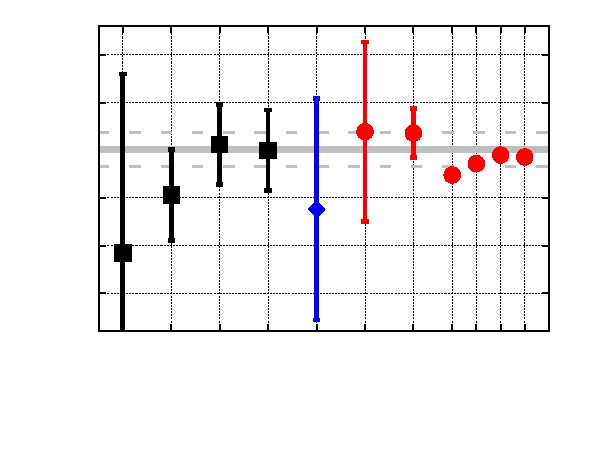
\includegraphics{PSPlainSizeComparison}}%
    \gplfronttext
  \end{picture}%
\endgroup

	\caption[Comparison of the PS-Plain particles average diameter with different techniques.]{Comparison of the PS-Plain average diameter obtained with different techniques, where the errorbars correspond to the expanded uncertainty ($k=2$). The circles correspond to results obtained with SAXS in the FCM beamline and the diamond to combined DCS measurements performed in NPL. The gray line defines the weighted mean of all the independent results, employing in the case of SAXS the shape scattering function result. The microscopy values are obtained from Belgian Service Métrologie-Metrologische Dienst (SMD), Swiss Federal Institute of Metrology (METAS) and Dutch Metrology Institute (VSL).}
	\label{fig:PSPlainSizeComparison}
\end{figure*}

The figure compares the PS-Plain diameter measured by the ensemble techniques SAXS and DCS and the imaging methods AFM and TSEM and presents the weighted mean value of all the independent results as a grey line, which corresponds to a diameter of 145.1 nm with an associated expanded uncertainty ($k=2$) of 1.8 nm. The SAXS results tend to larger values when modelling the scattering form factor, whilst the diameter obtained from the isoscattering points positions $I_i$ present values slightly smaller than the calculated mean value. However, the maximum deviation from the weighted mean is less than 2 $\%$.

The DCS result is obtained by a combined analysis of two complementary centrifuge configurations as detailed in section \ref{sec:DCS_experimental}, where figure \ref{fig:DCSCombinedStokes} depicts the dependency of the measured particle diameter on the density values for the two setups. The two setups measure the same diameter and density at the crossing point of the data, which occurs for a diameter of ($138.8\pm5.8$) nm and a density of ($1.052\pm0.010$) g cm$^{-3}$. The measured diameter fits within its uncertainty in the confidence interval of one standard deviation of the inter-laboratory comparison.

\begin{figure*}
	\begin{center}
		% GNUPLOT: LaTeX picture with Postscript
\begingroup
  \makeatletter
  \providecommand\color[2][]{%
    \GenericError{(gnuplot) \space\space\space\@spaces}{%
      Package color not loaded in conjunction with
      terminal option `colourtext'%
    }{See the gnuplot documentation for explanation.%
    }{Either use 'blacktext' in gnuplot or load the package
      color.sty in LaTeX.}%
    \renewcommand\color[2][]{}%
  }%
  \providecommand\includegraphics[2][]{%
    \GenericError{(gnuplot) \space\space\space\@spaces}{%
      Package graphicx or graphics not loaded%
    }{See the gnuplot documentation for explanation.%
    }{The gnuplot epslatex terminal needs graphicx.sty or graphics.sty.}%
    \renewcommand\includegraphics[2][]{}%
  }%
  \providecommand\rotatebox[2]{#2}%
  \@ifundefined{ifGPcolor}{%
    \newif\ifGPcolor
    \GPcolortrue
  }{}%
  \@ifundefined{ifGPblacktext}{%
    \newif\ifGPblacktext
    \GPblacktextfalse
  }{}%
  % define a \g@addto@macro without @ in the name:
  \let\gplgaddtomacro\g@addto@macro
  % define empty templates for all commands taking text:
  \gdef\gplbacktext{}%
  \gdef\gplfronttext{}%
  \makeatother
  \ifGPblacktext
    % no textcolor at all
    \def\colorrgb#1{}%
    \def\colorgray#1{}%
  \else
    % gray or color?
    \ifGPcolor
      \def\colorrgb#1{\color[rgb]{#1}}%
      \def\colorgray#1{\color[gray]{#1}}%
      \expandafter\def\csname LTw\endcsname{\color{white}}%
      \expandafter\def\csname LTb\endcsname{\color{black}}%
      \expandafter\def\csname LTa\endcsname{\color{black}}%
      \expandafter\def\csname LT0\endcsname{\color[rgb]{1,0,0}}%
      \expandafter\def\csname LT1\endcsname{\color[rgb]{0,1,0}}%
      \expandafter\def\csname LT2\endcsname{\color[rgb]{0,0,1}}%
      \expandafter\def\csname LT3\endcsname{\color[rgb]{1,0,1}}%
      \expandafter\def\csname LT4\endcsname{\color[rgb]{0,1,1}}%
      \expandafter\def\csname LT5\endcsname{\color[rgb]{1,1,0}}%
      \expandafter\def\csname LT6\endcsname{\color[rgb]{0,0,0}}%
      \expandafter\def\csname LT7\endcsname{\color[rgb]{1,0.3,0}}%
      \expandafter\def\csname LT8\endcsname{\color[rgb]{0.5,0.5,0.5}}%
    \else
      % gray
      \def\colorrgb#1{\color{black}}%
      \def\colorgray#1{\color[gray]{#1}}%
      \expandafter\def\csname LTw\endcsname{\color{white}}%
      \expandafter\def\csname LTb\endcsname{\color{black}}%
      \expandafter\def\csname LTa\endcsname{\color{black}}%
      \expandafter\def\csname LT0\endcsname{\color{black}}%
      \expandafter\def\csname LT1\endcsname{\color{black}}%
      \expandafter\def\csname LT2\endcsname{\color{black}}%
      \expandafter\def\csname LT3\endcsname{\color{black}}%
      \expandafter\def\csname LT4\endcsname{\color{black}}%
      \expandafter\def\csname LT5\endcsname{\color{black}}%
      \expandafter\def\csname LT6\endcsname{\color{black}}%
      \expandafter\def\csname LT7\endcsname{\color{black}}%
      \expandafter\def\csname LT8\endcsname{\color{black}}%
    \fi
  \fi
  \setlength{\unitlength}{0.0500bp}%
  \begin{picture}(5668.00,4534.00)%
    \gplgaddtomacro\gplbacktext{%
      \csname LTb\endcsname%
      \put(880,1232){\makebox(0,0)[r]{\strut{} 100}}%
      \csname LTb\endcsname%
      \put(880,1892){\makebox(0,0)[r]{\strut{} 150}}%
      \csname LTb\endcsname%
      \put(880,2553){\makebox(0,0)[r]{\strut{} 200}}%
      \csname LTb\endcsname%
      \put(880,3213){\makebox(0,0)[r]{\strut{} 250}}%
      \csname LTb\endcsname%
      \put(880,3873){\makebox(0,0)[r]{\strut{} 300}}%
      \csname LTb\endcsname%
      \put(1367,484){\makebox(0,0){\strut{} 1.02}}%
      \csname LTb\endcsname%
      \put(2077,484){\makebox(0,0){\strut{} 1.04}}%
      \csname LTb\endcsname%
      \put(2787,484){\makebox(0,0){\strut{} 1.06}}%
      \csname LTb\endcsname%
      \put(3496,484){\makebox(0,0){\strut{} 1.08}}%
      \csname LTb\endcsname%
      \put(4206,484){\makebox(0,0){\strut{} 1.1}}%
      \csname LTb\endcsname%
      \put(4916,484){\makebox(0,0){\strut{} 1.12}}%
      \put(176,2486){\rotatebox{-270}{\makebox(0,0){\strut{}PS-Plain diameter / nm}}}%
      \put(3141,154){\makebox(0,0){\strut{}PS-Plain density / g cm$^{-3}$}}%
    }%
    \gplgaddtomacro\gplfronttext{%
      \csname LTb\endcsname%
      \put(3793,4038){\makebox(0,0)[r]{\strut{}\smaller Standard disc}}%
      \csname LTb\endcsname%
      \put(3793,3708){\makebox(0,0)[r]{\strut{}\smaller Low density disc}}%
    }%
    \gplbacktext
    \put(0,0){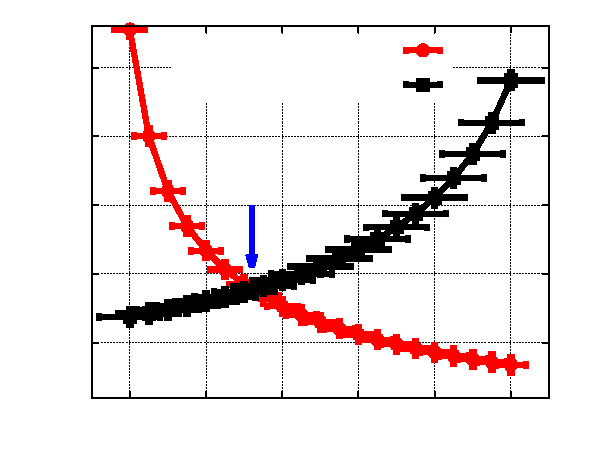
\includegraphics{DCSCombinedStokes}}%
    \gplfronttext
  \end{picture}%
\endgroup

	\end{center}
	\caption[Simultaneous size and density determination of the PS-Plain particles with a DCS combined approach.]{Dependence of the intensity-based modal Stokes' diameter on the particle density for the PS-Plain particles analysed in H$_2$O-sucrose (black) and D$_2$O-sucrose (red) gradients. The arrow indicates the crossing point of the data, where the two setups measure the same diameter and density of the colloid. This occurs for a diameter of ($138.8\pm5.8$) nm and a density of ($1.052\pm0.010$) g cm$^{-3}$}
	\label{fig:DCSCombinedStokes}
\end{figure*}

All the techniques are in very good agreement, even considering that they are based on different physical principles. The improvement in accuracy for the size determination with SAXS by using the shape scattering function approach is further sustained by this comparison. 

This improvement was confirmed by employing the same approach with the PS-COOH colloids. The diameter obtained from the core-shell model fit in chapter \ref{chap:density_gradient_SAXS} is ($99.4\pm5.6$) nm, while the value obtained from the shape scattering function calculation is ($101.4\pm2.4$) nm. Again, the uncertainty associated to the size decreases by $\sim 60\;\%$, whilst it is still in accordance with the diameter obtained with the isoscattering points positions of 101.0 nm with a standard deviation of 1.1 nm. 

Due to the low polydispersity of the PMMA-COOH particles and their homogenous composition, a spherical form factor fit to the single-contrast scattering curve provides already a very accurate diameter ($186.5\pm2.3$) nm. In this case, contrast variation experiments in SAXS show no advantages.

\subsection{Particle size distribution of the PS-Plain particles}

An important attribute of polymeric colloids is their polydispersity, as the suitability for specific applications depends on their spread in size. For example, colloids are known to induce different inflammatory responses depending on their size \citep{kusaka_effect_2014}.

\begin{figure}
	\begin{center}
		% GNUPLOT: LaTeX picture with Postscript
\begingroup
  \makeatletter
  \providecommand\color[2][]{%
    \GenericError{(gnuplot) \space\space\space\@spaces}{%
      Package color not loaded in conjunction with
      terminal option `colourtext'%
    }{See the gnuplot documentation for explanation.%
    }{Either use 'blacktext' in gnuplot or load the package
      color.sty in LaTeX.}%
    \renewcommand\color[2][]{}%
  }%
  \providecommand\includegraphics[2][]{%
    \GenericError{(gnuplot) \space\space\space\@spaces}{%
      Package graphicx or graphics not loaded%
    }{See the gnuplot documentation for explanation.%
    }{The gnuplot epslatex terminal needs graphicx.sty or graphics.sty.}%
    \renewcommand\includegraphics[2][]{}%
  }%
  \providecommand\rotatebox[2]{#2}%
  \@ifundefined{ifGPcolor}{%
    \newif\ifGPcolor
    \GPcolortrue
  }{}%
  \@ifundefined{ifGPblacktext}{%
    \newif\ifGPblacktext
    \GPblacktextfalse
  }{}%
  % define a \g@addto@macro without @ in the name:
  \let\gplgaddtomacro\g@addto@macro
  % define empty templates for all commands taking text:
  \gdef\gplbacktext{}%
  \gdef\gplfronttext{}%
  \makeatother
  \ifGPblacktext
    % no textcolor at all
    \def\colorrgb#1{}%
    \def\colorgray#1{}%
  \else
    % gray or color?
    \ifGPcolor
      \def\colorrgb#1{\color[rgb]{#1}}%
      \def\colorgray#1{\color[gray]{#1}}%
      \expandafter\def\csname LTw\endcsname{\color{white}}%
      \expandafter\def\csname LTb\endcsname{\color{black}}%
      \expandafter\def\csname LTa\endcsname{\color{black}}%
      \expandafter\def\csname LT0\endcsname{\color[rgb]{1,0,0}}%
      \expandafter\def\csname LT1\endcsname{\color[rgb]{0,1,0}}%
      \expandafter\def\csname LT2\endcsname{\color[rgb]{0,0,1}}%
      \expandafter\def\csname LT3\endcsname{\color[rgb]{1,0,1}}%
      \expandafter\def\csname LT4\endcsname{\color[rgb]{0,1,1}}%
      \expandafter\def\csname LT5\endcsname{\color[rgb]{1,1,0}}%
      \expandafter\def\csname LT6\endcsname{\color[rgb]{0,0,0}}%
      \expandafter\def\csname LT7\endcsname{\color[rgb]{1,0.3,0}}%
      \expandafter\def\csname LT8\endcsname{\color[rgb]{0.5,0.5,0.5}}%
    \else
      % gray
      \def\colorrgb#1{\color{black}}%
      \def\colorgray#1{\color[gray]{#1}}%
      \expandafter\def\csname LTw\endcsname{\color{white}}%
      \expandafter\def\csname LTb\endcsname{\color{black}}%
      \expandafter\def\csname LTa\endcsname{\color{black}}%
      \expandafter\def\csname LT0\endcsname{\color{black}}%
      \expandafter\def\csname LT1\endcsname{\color{black}}%
      \expandafter\def\csname LT2\endcsname{\color{black}}%
      \expandafter\def\csname LT3\endcsname{\color{black}}%
      \expandafter\def\csname LT4\endcsname{\color{black}}%
      \expandafter\def\csname LT5\endcsname{\color{black}}%
      \expandafter\def\csname LT6\endcsname{\color{black}}%
      \expandafter\def\csname LT7\endcsname{\color{black}}%
      \expandafter\def\csname LT8\endcsname{\color{black}}%
    \fi
  \fi
  \setlength{\unitlength}{0.0500bp}%
  \begin{picture}(5668.00,4534.00)%
    \gplgaddtomacro\gplbacktext{%
      \csname LTb\endcsname%
      \put(814,777){\makebox(0,0)[r]{\strut{} 0}}%
      \csname LTb\endcsname%
      \put(814,1359){\makebox(0,0)[r]{\strut{} 0.2}}%
      \csname LTb\endcsname%
      \put(814,1941){\makebox(0,0)[r]{\strut{} 0.4}}%
      \csname LTb\endcsname%
      \put(814,2523){\makebox(0,0)[r]{\strut{} 0.6}}%
      \csname LTb\endcsname%
      \put(814,3105){\makebox(0,0)[r]{\strut{} 0.8}}%
      \csname LTb\endcsname%
      \put(814,3687){\makebox(0,0)[r]{\strut{} 1}}%
      \csname LTb\endcsname%
      \put(814,4269){\makebox(0,0)[r]{\strut{} 1.2}}%
      \csname LTb\endcsname%
      \put(946,484){\makebox(0,0){\strut{} 80}}%
      \csname LTb\endcsname%
      \put(1732,484){\makebox(0,0){\strut{} 100}}%
      \csname LTb\endcsname%
      \put(2519,484){\makebox(0,0){\strut{} 120}}%
      \csname LTb\endcsname%
      \put(3305,484){\makebox(0,0){\strut{} 140}}%
      \csname LTb\endcsname%
      \put(4091,484){\makebox(0,0){\strut{} 160}}%
      \csname LTb\endcsname%
      \put(4878,484){\makebox(0,0){\strut{} 180}}%
      \put(176,2486){\rotatebox{-270}{\makebox(0,0){\strut{}Frequency / a.u.}}}%
      \put(3108,154){\makebox(0,0){\strut{}Size / nm}}%
    }%
    \gplgaddtomacro\gplfronttext{%
      \csname LTb\endcsname%
      \put(2371,4046){\makebox(0,0)[r]{\strut{}TSEM}}%
      \csname LTb\endcsname%
      \put(2371,3716){\makebox(0,0)[r]{\strut{}Shape Factor SAXS}}%
      \csname LTb\endcsname%
      \put(2371,3386){\makebox(0,0)[r]{\strut{}Standard DCS}}%
      \csname LTb\endcsname%
      \put(2371,3056){\makebox(0,0)[r]{\strut{}Low density DCS}}%
    }%
    \gplbacktext
    \put(0,0){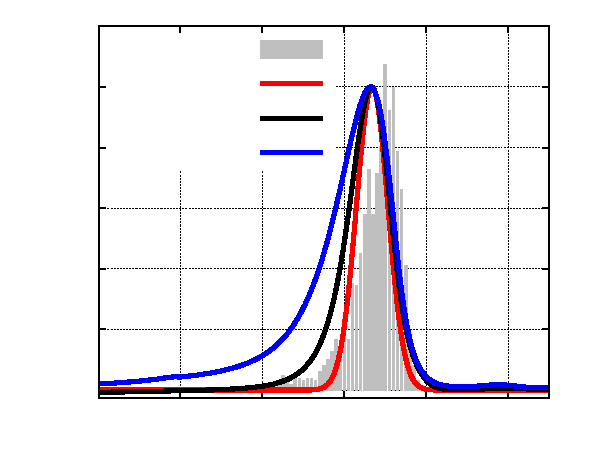
\includegraphics{PSPlainSizeDistribution}}%
    \gplfronttext
  \end{picture}%
\endgroup

	\end{center}
	\caption[Number-weighted size distribution of the PS-Plain particles.]{Number-weighted size distribution of the PS-Plain particles measured by DCS, TSEM \citep{nicolet_inter-laboratory_2016} and SAXS with the shape scattering function approach.}
	\label{fig:PSPlainSizeDistribution}
\end{figure}

The SAXS results determine a polydispersity degree $p_d$ for the PS-Plain colloids of 6.1 $\%$, which is an indicator of a very monodisperse distribution, as also suggested by the regular minima observed in figure \ref{fig:PSPlainSingleContrastSAXS}. Particle polydispersities measured by DCS are also low as observed in figure \ref{fig:PSPlainSizeDistribution}, ranging from 7.8 $\%$ measured with the standard set up, to 11.3 $\%$ measured with the low density disc setup. The standard setup appears therefore to achieve a higher resolution size distribution. The size distribution measured by TSEM with a $p_d$ of 8.3 $\%$ shows good agreement with the ensemble techniques.

The measurements obtained by AFM provide polydispersity degrees larger than 10 $\%$ \citep{nicolet_inter-laboratory_2016} and, therefore, slightly broader size distributions than those calculated by SAXS, TSEM and standard DCS. This can be in part attributed to the low statistics that typically affect imaging methods, along with artefacts associated with the posterior analysis.

For instance, in the TSEM images \citep{nicolet_inter-laboratory_2016}, smaller and larger populations with different contrasts have been observed which could affect the evaluation of the density measured by ensemble techniques in the following section \ref{sec:physical_density}, as the particle average density might vary. Indeed, when a bimodal distribution is used to analyse the SAXS shape scattering function of the PS-Plain particles, a second size population is found at 101 nm in agreement with TSEM, while the main mode maintains a $p_d$ of ca. 5 $\%$.

\section{Considerations about scattering data evaluation}

In the previous section, the mean diameter of polymeric nanoparticles was obtained using two different model-free approaches, i.e. the isoscattering point and the shape scattering function. The method employed to analyse the scattering curves measured with the continuous contrast variation technique in SAXS affects the size determination and its accuracy, as suggested by the results. Following, a discussion about both approaches is presented based on the scattering data shown in figure \ref{fig:PSPlainContinuousSAXS}.

\subsection{Shape scattering function formalism}
The shape scattering function obtained by density gradient contrast variation has been demonstrated as a powerful technique which can provide precise information about the size distribution and shape of the colloid by fitting a simple form factor.

\begin{figure}
	\begin{center}
		% GNUPLOT: LaTeX picture with Postscript
\begingroup
  \makeatletter
  \providecommand\color[2][]{%
    \GenericError{(gnuplot) \space\space\space\@spaces}{%
      Package color not loaded in conjunction with
      terminal option `colourtext'%
    }{See the gnuplot documentation for explanation.%
    }{Either use 'blacktext' in gnuplot or load the package
      color.sty in LaTeX.}%
    \renewcommand\color[2][]{}%
  }%
  \providecommand\includegraphics[2][]{%
    \GenericError{(gnuplot) \space\space\space\@spaces}{%
      Package graphicx or graphics not loaded%
    }{See the gnuplot documentation for explanation.%
    }{The gnuplot epslatex terminal needs graphicx.sty or graphics.sty.}%
    \renewcommand\includegraphics[2][]{}%
  }%
  \providecommand\rotatebox[2]{#2}%
  \@ifundefined{ifGPcolor}{%
    \newif\ifGPcolor
    \GPcolortrue
  }{}%
  \@ifundefined{ifGPblacktext}{%
    \newif\ifGPblacktext
    \GPblacktextfalse
  }{}%
  % define a \g@addto@macro without @ in the name:
  \let\gplgaddtomacro\g@addto@macro
  % define empty templates for all commands taking text:
  \gdef\gplbacktext{}%
  \gdef\gplfronttext{}%
  \makeatother
  \ifGPblacktext
    % no textcolor at all
    \def\colorrgb#1{}%
    \def\colorgray#1{}%
  \else
    % gray or color?
    \ifGPcolor
      \def\colorrgb#1{\color[rgb]{#1}}%
      \def\colorgray#1{\color[gray]{#1}}%
      \expandafter\def\csname LTw\endcsname{\color{white}}%
      \expandafter\def\csname LTb\endcsname{\color{black}}%
      \expandafter\def\csname LTa\endcsname{\color{black}}%
      \expandafter\def\csname LT0\endcsname{\color[rgb]{1,0,0}}%
      \expandafter\def\csname LT1\endcsname{\color[rgb]{0,1,0}}%
      \expandafter\def\csname LT2\endcsname{\color[rgb]{0,0,1}}%
      \expandafter\def\csname LT3\endcsname{\color[rgb]{1,0,1}}%
      \expandafter\def\csname LT4\endcsname{\color[rgb]{0,1,1}}%
      \expandafter\def\csname LT5\endcsname{\color[rgb]{1,1,0}}%
      \expandafter\def\csname LT6\endcsname{\color[rgb]{0,0,0}}%
      \expandafter\def\csname LT7\endcsname{\color[rgb]{1,0.3,0}}%
      \expandafter\def\csname LT8\endcsname{\color[rgb]{0.5,0.5,0.5}}%
    \else
      % gray
      \def\colorrgb#1{\color{black}}%
      \def\colorgray#1{\color[gray]{#1}}%
      \expandafter\def\csname LTw\endcsname{\color{white}}%
      \expandafter\def\csname LTb\endcsname{\color{black}}%
      \expandafter\def\csname LTa\endcsname{\color{black}}%
      \expandafter\def\csname LT0\endcsname{\color{black}}%
      \expandafter\def\csname LT1\endcsname{\color{black}}%
      \expandafter\def\csname LT2\endcsname{\color{black}}%
      \expandafter\def\csname LT3\endcsname{\color{black}}%
      \expandafter\def\csname LT4\endcsname{\color{black}}%
      \expandafter\def\csname LT5\endcsname{\color{black}}%
      \expandafter\def\csname LT6\endcsname{\color{black}}%
      \expandafter\def\csname LT7\endcsname{\color{black}}%
      \expandafter\def\csname LT8\endcsname{\color{black}}%
    \fi
  \fi
  \setlength{\unitlength}{0.0500bp}%
  \begin{picture}(5668.00,4534.00)%
    \gplgaddtomacro\gplbacktext{%
      \csname LTb\endcsname%
      \put(748,866){\makebox(0,0)[r]{\strut{} 140}}%
      \csname LTb\endcsname%
      \put(748,1514){\makebox(0,0)[r]{\strut{} 142}}%
      \csname LTb\endcsname%
      \put(748,2162){\makebox(0,0)[r]{\strut{} 144}}%
      \csname LTb\endcsname%
      \put(748,2811){\makebox(0,0)[r]{\strut{} 146}}%
      \csname LTb\endcsname%
      \put(748,3459){\makebox(0,0)[r]{\strut{} 148}}%
      \csname LTb\endcsname%
      \put(748,4107){\makebox(0,0)[r]{\strut{} 150}}%
      \csname LTb\endcsname%
      \put(880,484){\makebox(0,0){\strut{} 0}}%
      \csname LTb\endcsname%
      \put(1507,484){\makebox(0,0){\strut{} 5}}%
      \csname LTb\endcsname%
      \put(2135,484){\makebox(0,0){\strut{} 10}}%
      \csname LTb\endcsname%
      \put(2762,484){\makebox(0,0){\strut{} 15}}%
      \csname LTb\endcsname%
      \put(3389,484){\makebox(0,0){\strut{} 20}}%
      \csname LTb\endcsname%
      \put(4016,484){\makebox(0,0){\strut{} 25}}%
      \csname LTb\endcsname%
      \put(4644,484){\makebox(0,0){\strut{} 30}}%
      \csname LTb\endcsname%
      \put(5271,484){\makebox(0,0){\strut{} 35}}%
      \put(176,2486){\rotatebox{-270}{\makebox(0,0){\strut{}Diameter / nm}}}%
      \put(3075,154){\makebox(0,0){\strut{}Number of scattering curves}}%
    }%
    \gplgaddtomacro\gplfronttext{%
    }%
    \gplbacktext
    \put(0,0){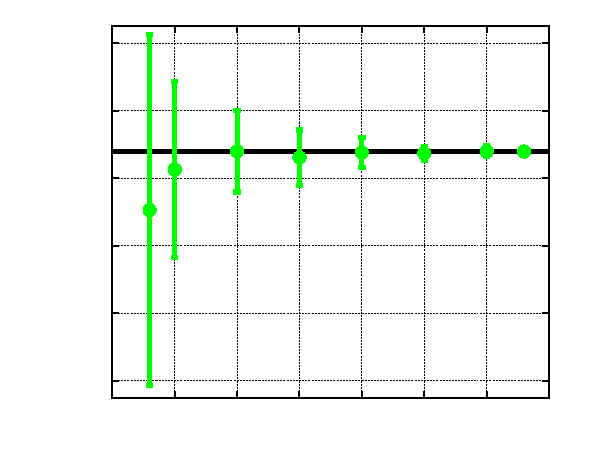
\includegraphics{ResonantTermSimulationNumber}}%
    \gplfronttext
  \end{picture}%
\endgroup

	\end{center}
\caption[Diameter of the PS-Plain particles obtained from the shape scattering function as a function of the number of scattering curves.]{Diameter of the PS-Plain particles as a function of the number of scattering curves used in the shape scattering function calculation. The horizontal line shows a diameter of 146.8 nm.}
\label{fig:ResonantTermSimulationNumber}
\end{figure}

However, an accurate determination of the suspending medium density for each scattering curve is required, due to the increased uncertainties \citep{lefebvre_propagation_2000} that can arise from the resolution of the system of linear equations described in section \ref{sec:basic_functions_theory}.

Besides, a minimum of 3 scattering curves measured at different contrasts is necessary to obtain the resonant term, although an increasing number improves the determination of the size distribution. This issue has been addressed with the experimental data of the PS-Plain colloids measured by the density gradient contrast variation. From the 40 experimental curves, only a limited number $N$ was randomly selected to compute the shape scattering function, while this process was repeated 100 times. The mean diameter obtained from this data set and its statistical standard deviation are plotted in figure \ref{fig:ResonantTermSimulationNumber} as a function of $N$.

The effect of increasing the number of measured contrasts evidences that the result tends asymptotically to the value of 146.8 nm discussed in section \ref{sec:size_validation} and the standard deviation of the 100 iterations decreases for large $N$, e.g. the associated uncertainty is reduced. This outcome emphasizes further the advantages of the continuous contrast variation technique due to the large number of scattering curves at different contrasts which can be easily measured.

In summary, it has been demonstrated that the possibility to determine the particle size distribution by the shape scattering function is a clear improvement to single-contrast SAXS techniques reducing relevantly the uncertainty, although an accurate determination of the contrast and a relatively high number of scattering curves are required. 

\subsection{Isoscattering point approach}

The theory defines $q^{\star}$ as a morphological parameter independent of the suspending medium density, which is a enormous practical advantage as it can be located without the proper calibration of the contrast. In cases where the composition of the buffer is unknown or the density of the solvent cannot be properly calibrated, the isoscattering point position might still be quantifiable by calculating the relative standard deviation of all the measured scattering curves. 

In order to obtain reliable results, a proper subtraction of the solvent scattering must be performed. It is clear in figure \ref{fig:PSPlainContinuousSAXSIsopoint} that the correction of the solvent contribution to the scattering intensity plays an important role in the determination of the $q^{\star}$ values as the curve shifts to smaller $q$-values when subtracting the solvent background. Although this effect is larger at high $q$-values, the solvent background influences the position of all the isoscattering points as summarized in table \ref{tab:isoscattering_points}. 

\begin{table*}
	\centering
	\begin{tabular}{l||cc|cc|c}
		 & \multicolumn{2}{c}{Raw data} & \multicolumn{2}{c}{Corrected data} & Deviation\\
		 \hline
		 & \( q^{\star} \) (nm\(^{-1}\))    &  Diameter (nm) & \( q^{\star}\) (nm\(^{-1}\))    &  Diameter (nm) & $\%$ \\
		\hline
		 \(q^{\star}_1\) &  0.0633 & 142.0 &  0.0631 & 142.4 & 0.3 \\
		 \(q^{\star}_2\) &  0.1088 & 142.0 &  0.1076 & 143.6 & 1.1   \\
		 \(q^{\star}_3\) &  0.1537 & 141.9 &  0.1510 & 144.4 & 1.7    \\
		 \(q^{\star}_4\) &  0.206  & 136.6 &  0.195  & 144.3 & 5.3     \\
		\end{tabular}
	\caption[Isoscattering points position and their corresponding particle diameter.]{Isoscattering points position and the corresponding particle diameter for the scattering curves before and after background correction. The diameter deviation between both values is also shown, with larger deviation for higher $q$-values.}
	\label{tab:isoscattering_points}
\end{table*}

It has been discussed before in this work that the polydispersity of the latex and its deviation from the spherical shape influence the position and diffuseness of $q^{\star}$, principally at high $q$-values. This can disturb the size determination for polymeric particles with broad size distributions and limit the applicability of this technique. 

In order to prove the isoscattering point dependency on the particle polydispersity, the diameter obtained from the first isoscattering point position is simulated for three core-shell particle with different core-to-size ratios, as depicted in figure \ref{fig:IsopointSimulationPolydispersity}. The deviation of the calculated size from the nominal size becomes larger for increasing particle polydispersities, reaching size deviations up to 8 $\%$ at $p_d = 30\;\%$. Moreover, the size deviation behaves differently depending on the internal structure of the particle, tending to larger deviations for thicker shells and positive deviations for thinner ones.

\begin{figure*}%[htbp]
	\centering
		\subfloat[Polydispersity effects]{\resizebox{0.44\linewidth}{!}{\figfont{13pt}% GNUPLOT: LaTeX picture with Postscript
\begingroup
  \makeatletter
  \providecommand\color[2][]{%
    \GenericError{(gnuplot) \space\space\space\@spaces}{%
      Package color not loaded in conjunction with
      terminal option `colourtext'%
    }{See the gnuplot documentation for explanation.%
    }{Either use 'blacktext' in gnuplot or load the package
      color.sty in LaTeX.}%
    \renewcommand\color[2][]{}%
  }%
  \providecommand\includegraphics[2][]{%
    \GenericError{(gnuplot) \space\space\space\@spaces}{%
      Package graphicx or graphics not loaded%
    }{See the gnuplot documentation for explanation.%
    }{The gnuplot epslatex terminal needs graphicx.sty or graphics.sty.}%
    \renewcommand\includegraphics[2][]{}%
  }%
  \providecommand\rotatebox[2]{#2}%
  \@ifundefined{ifGPcolor}{%
    \newif\ifGPcolor
    \GPcolortrue
  }{}%
  \@ifundefined{ifGPblacktext}{%
    \newif\ifGPblacktext
    \GPblacktextfalse
  }{}%
  % define a \g@addto@macro without @ in the name:
  \let\gplgaddtomacro\g@addto@macro
  % define empty templates for all commands taking text:
  \gdef\gplbacktext{}%
  \gdef\gplfronttext{}%
  \makeatother
  \ifGPblacktext
    % no textcolor at all
    \def\colorrgb#1{}%
    \def\colorgray#1{}%
  \else
    % gray or color?
    \ifGPcolor
      \def\colorrgb#1{\color[rgb]{#1}}%
      \def\colorgray#1{\color[gray]{#1}}%
      \expandafter\def\csname LTw\endcsname{\color{white}}%
      \expandafter\def\csname LTb\endcsname{\color{black}}%
      \expandafter\def\csname LTa\endcsname{\color{black}}%
      \expandafter\def\csname LT0\endcsname{\color[rgb]{1,0,0}}%
      \expandafter\def\csname LT1\endcsname{\color[rgb]{0,1,0}}%
      \expandafter\def\csname LT2\endcsname{\color[rgb]{0,0,1}}%
      \expandafter\def\csname LT3\endcsname{\color[rgb]{1,0,1}}%
      \expandafter\def\csname LT4\endcsname{\color[rgb]{0,1,1}}%
      \expandafter\def\csname LT5\endcsname{\color[rgb]{1,1,0}}%
      \expandafter\def\csname LT6\endcsname{\color[rgb]{0,0,0}}%
      \expandafter\def\csname LT7\endcsname{\color[rgb]{1,0.3,0}}%
      \expandafter\def\csname LT8\endcsname{\color[rgb]{0.5,0.5,0.5}}%
    \else
      % gray
      \def\colorrgb#1{\color{black}}%
      \def\colorgray#1{\color[gray]{#1}}%
      \expandafter\def\csname LTw\endcsname{\color{white}}%
      \expandafter\def\csname LTb\endcsname{\color{black}}%
      \expandafter\def\csname LTa\endcsname{\color{black}}%
      \expandafter\def\csname LT0\endcsname{\color{black}}%
      \expandafter\def\csname LT1\endcsname{\color{black}}%
      \expandafter\def\csname LT2\endcsname{\color{black}}%
      \expandafter\def\csname LT3\endcsname{\color{black}}%
      \expandafter\def\csname LT4\endcsname{\color{black}}%
      \expandafter\def\csname LT5\endcsname{\color{black}}%
      \expandafter\def\csname LT6\endcsname{\color{black}}%
      \expandafter\def\csname LT7\endcsname{\color{black}}%
      \expandafter\def\csname LT8\endcsname{\color{black}}%
    \fi
  \fi
  \setlength{\unitlength}{0.0500bp}%
  \begin{picture}(5668.00,4534.00)%
    \gplgaddtomacro\gplbacktext{%
      \csname LTb\endcsname%
      \put(682,704){\makebox(0,0)[r]{\strut{}-8}}%
      \csname LTb\endcsname%
      \put(682,1028){\makebox(0,0)[r]{\strut{}-7}}%
      \csname LTb\endcsname%
      \put(682,1352){\makebox(0,0)[r]{\strut{}-6}}%
      \csname LTb\endcsname%
      \put(682,1676){\makebox(0,0)[r]{\strut{}-5}}%
      \csname LTb\endcsname%
      \put(682,2000){\makebox(0,0)[r]{\strut{}-4}}%
      \csname LTb\endcsname%
      \put(682,2324){\makebox(0,0)[r]{\strut{}-3}}%
      \csname LTb\endcsname%
      \put(682,2649){\makebox(0,0)[r]{\strut{}-2}}%
      \csname LTb\endcsname%
      \put(682,2973){\makebox(0,0)[r]{\strut{}-1}}%
      \csname LTb\endcsname%
      \put(682,3297){\makebox(0,0)[r]{\strut{} 0}}%
      \csname LTb\endcsname%
      \put(682,3621){\makebox(0,0)[r]{\strut{} 1}}%
      \csname LTb\endcsname%
      \put(682,3945){\makebox(0,0)[r]{\strut{} 2}}%
      \csname LTb\endcsname%
      \put(682,4269){\makebox(0,0)[r]{\strut{} 3}}%
      \csname LTb\endcsname%
      \put(814,484){\makebox(0,0){\strut{} 0}}%
      \csname LTb\endcsname%
      \put(1557,484){\makebox(0,0){\strut{} 5}}%
      \csname LTb\endcsname%
      \put(2300,484){\makebox(0,0){\strut{} 10}}%
      \csname LTb\endcsname%
      \put(3043,484){\makebox(0,0){\strut{} 15}}%
      \csname LTb\endcsname%
      \put(3785,484){\makebox(0,0){\strut{} 20}}%
      \csname LTb\endcsname%
      \put(4528,484){\makebox(0,0){\strut{} 25}}%
      \csname LTb\endcsname%
      \put(5271,484){\makebox(0,0){\strut{} 30}}%
      \put(176,2486){\rotatebox{-270}{\makebox(0,0){\strut{}Isoscattering point deviation / $\%$}}}%
      \put(3042,154){\makebox(0,0){\strut{}Polydispersity degree / $\%$}}%
    }%
    \gplgaddtomacro\gplfronttext{%
      \csname LTb\endcsname%
      \put(1715,2214){\makebox(0,0){\strut{}Ratio $\sfrac{R_{\text{core}}}{R}$}}%
      \csname LTb\endcsname%
      \put(1816,1939){\makebox(0,0)[r]{\strut{}69 $\%$}}%
      \csname LTb\endcsname%
      \put(1816,1609){\makebox(0,0)[r]{\strut{}83 $\%$}}%
      \csname LTb\endcsname%
      \put(1816,1279){\makebox(0,0)[r]{\strut{}94 $\%$}}%
    }%
    \gplbacktext
    \put(0,0){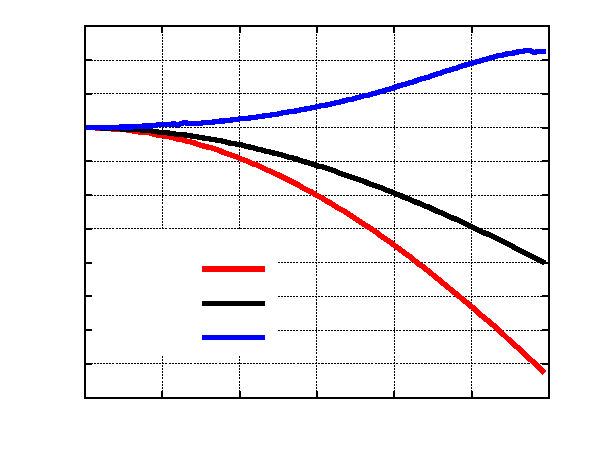
\includegraphics{IsopointSimulationPolydispersity}}%
    \gplfronttext
  \end{picture}%
\endgroup
}\label{fig:IsopointSimulationPolydispersity}}
		\subfloat[Solvent electron density range]{\resizebox{0.44\linewidth}{!}{\figfont{13pt}% GNUPLOT: LaTeX picture with Postscript
\begingroup
  \makeatletter
  \providecommand\color[2][]{%
    \GenericError{(gnuplot) \space\space\space\@spaces}{%
      Package color not loaded in conjunction with
      terminal option `colourtext'%
    }{See the gnuplot documentation for explanation.%
    }{Either use 'blacktext' in gnuplot or load the package
      color.sty in LaTeX.}%
    \renewcommand\color[2][]{}%
  }%
  \providecommand\includegraphics[2][]{%
    \GenericError{(gnuplot) \space\space\space\@spaces}{%
      Package graphicx or graphics not loaded%
    }{See the gnuplot documentation for explanation.%
    }{The gnuplot epslatex terminal needs graphicx.sty or graphics.sty.}%
    \renewcommand\includegraphics[2][]{}%
  }%
  \providecommand\rotatebox[2]{#2}%
  \@ifundefined{ifGPcolor}{%
    \newif\ifGPcolor
    \GPcolortrue
  }{}%
  \@ifundefined{ifGPblacktext}{%
    \newif\ifGPblacktext
    \GPblacktextfalse
  }{}%
  % define a \g@addto@macro without @ in the name:
  \let\gplgaddtomacro\g@addto@macro
  % define empty templates for all commands taking text:
  \gdef\gplbacktext{}%
  \gdef\gplfronttext{}%
  \makeatother
  \ifGPblacktext
    % no textcolor at all
    \def\colorrgb#1{}%
    \def\colorgray#1{}%
  \else
    % gray or color?
    \ifGPcolor
      \def\colorrgb#1{\color[rgb]{#1}}%
      \def\colorgray#1{\color[gray]{#1}}%
      \expandafter\def\csname LTw\endcsname{\color{white}}%
      \expandafter\def\csname LTb\endcsname{\color{black}}%
      \expandafter\def\csname LTa\endcsname{\color{black}}%
      \expandafter\def\csname LT0\endcsname{\color[rgb]{1,0,0}}%
      \expandafter\def\csname LT1\endcsname{\color[rgb]{0,1,0}}%
      \expandafter\def\csname LT2\endcsname{\color[rgb]{0,0,1}}%
      \expandafter\def\csname LT3\endcsname{\color[rgb]{1,0,1}}%
      \expandafter\def\csname LT4\endcsname{\color[rgb]{0,1,1}}%
      \expandafter\def\csname LT5\endcsname{\color[rgb]{1,1,0}}%
      \expandafter\def\csname LT6\endcsname{\color[rgb]{0,0,0}}%
      \expandafter\def\csname LT7\endcsname{\color[rgb]{1,0.3,0}}%
      \expandafter\def\csname LT8\endcsname{\color[rgb]{0.5,0.5,0.5}}%
    \else
      % gray
      \def\colorrgb#1{\color{black}}%
      \def\colorgray#1{\color[gray]{#1}}%
      \expandafter\def\csname LTw\endcsname{\color{white}}%
      \expandafter\def\csname LTb\endcsname{\color{black}}%
      \expandafter\def\csname LTa\endcsname{\color{black}}%
      \expandafter\def\csname LT0\endcsname{\color{black}}%
      \expandafter\def\csname LT1\endcsname{\color{black}}%
      \expandafter\def\csname LT2\endcsname{\color{black}}%
      \expandafter\def\csname LT3\endcsname{\color{black}}%
      \expandafter\def\csname LT4\endcsname{\color{black}}%
      \expandafter\def\csname LT5\endcsname{\color{black}}%
      \expandafter\def\csname LT6\endcsname{\color{black}}%
      \expandafter\def\csname LT7\endcsname{\color{black}}%
      \expandafter\def\csname LT8\endcsname{\color{black}}%
    \fi
  \fi
  \setlength{\unitlength}{0.0500bp}%
  \begin{picture}(5668.00,4534.00)%
    \gplgaddtomacro\gplbacktext{%
      \csname LTb\endcsname%
      \put(946,1014){\makebox(0,0)[r]{\strut{}-0.5}}%
      \csname LTb\endcsname%
      \put(946,1789){\makebox(0,0)[r]{\strut{} 0}}%
      \csname LTb\endcsname%
      \put(946,2564){\makebox(0,0)[r]{\strut{} 0.5}}%
      \csname LTb\endcsname%
      \put(946,3339){\makebox(0,0)[r]{\strut{} 1}}%
      \csname LTb\endcsname%
      \put(946,4114){\makebox(0,0)[r]{\strut{} 1.5}}%
      \csname LTb\endcsname%
      \put(1078,484){\makebox(0,0){\strut{} 330}}%
      \csname LTb\endcsname%
      \put(1677,484){\makebox(0,0){\strut{} 340}}%
      \csname LTb\endcsname%
      \put(2276,484){\makebox(0,0){\strut{} 350}}%
      \csname LTb\endcsname%
      \put(2875,484){\makebox(0,0){\strut{} 360}}%
      \csname LTb\endcsname%
      \put(3474,484){\makebox(0,0){\strut{} 370}}%
      \csname LTb\endcsname%
      \put(4073,484){\makebox(0,0){\strut{} 380}}%
      \csname LTb\endcsname%
      \put(4672,484){\makebox(0,0){\strut{} 390}}%
      \csname LTb\endcsname%
      \put(5271,484){\makebox(0,0){\strut{} 400}}%
      \put(176,2486){\rotatebox{-270}{\makebox(0,0){\strut{}Deviation / $\%$}}}%
      \put(3174,154){\makebox(0,0){\strut{}$\rho_{max}$ / nm$^{-3}$}}%
    }%
    \gplgaddtomacro\gplfronttext{%
    }%
    \gplbacktext
    \put(0,0){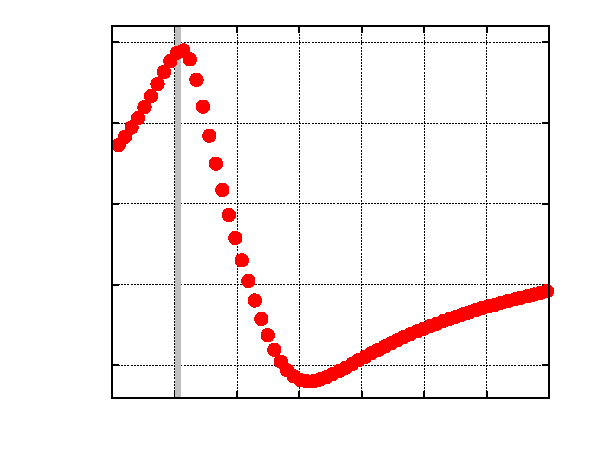
\includegraphics{IsopointSimulationRange}}%
    \gplfronttext
  \end{picture}%
\endgroup
}\label{fig:IsopointSimulationRange}}
	\caption[Deviation of the size of the PS-Plain particles obtained with $q_1^{\star}$ from the nominal value.]{Deviation of the size of the PS-Plain particles calculated using the $q_1^{\star}$ position from the nominal value depending on a) the size polydispersity of core-shell particles with different core-to-size ratios or b) the solvent electron density range employed in the experiment, where  $\rho_e \in (330\;\mbox{nm}^{-3}, \rho_{\text{max}})$.}

\end{figure*}

This work demonstrates also that the $q^{\star}$ value determined with the previously described method depends on the range of solvent densities used in the contrast variation experiment. For this purpose,  a contrast variation experiment with 10 different solvent densities was simulated for a polymeric particle with the morphology and size distribution obtained with the core-shell model in section \ref{sec:size_validation}. Using a lower bound to the contrast range of $\rho_{\text{min}}=330$ nm$^{-3}$ and increasing systematically the upper limit, it is shown in figure \ref{fig:IsopointSimulationRange} that the calculated result deviates from the nominal value up to 1.5 $\%$. 

In this example, the largest deviations occur when the average density of the latex i.e. match point (depicted as a vertical line in figure \ref{fig:IsopointSimulationRange}) is excluded from the experimental contrast range or when $\rho_{\text{max}}$ is close to this matching density. This observation conflicts partly with the initial intuition that this technique is independent of the experimental procedure, although this problem can be avoided by selecting the solvent electron density range skillfully i.e. equidistantly distributed around the match point. This could be one explanation behind the slight size differences observed in figure \ref{fig:PSPlainSizeComparison} between the issocattering approach and the other SAXS results.

The isoscattering point approach to contrast variation SAXS data evaluation presents certain assets which can not be ignored. For instance, the independence of $q^{\star}$ from the sample contrast facilitates its easy application, although the solvent electron density range must be chosen with care and always around the average electron density of the particle to maximize its accuracy. On the other hand, the diffuseness of the isoscattering point position due to the polydispersity and ellipticity of the sample arises as an indisputable drawback.

\section{Determination of the particle mass density}
\label{sec:physical_density}
In contrast variation SAXS, the solvent electron density which matches the average electron density of the particle $\rho_0$ corresponds to a minimum in the intensity of the scattering curve  according to expression \ref{eq:I0}. In order to quantify the particle density, the scattering intensity of the PS-Plain particles at zero angle $I(0)$ is examined along the contrast range of the experiment as shown in figure \ref{fig:PSPlainAverageDensity}. The value of $I(0)$ was determined by extrapolation to $q\rightarrow 0$ using a spherical form factor function fitted to the available range before the first minimum, as discussed in section \ref{sec:guinier_analysis}. The parabolic fit to the data is plotted as a black line in figure \ref{fig:PSPlainAverageDensity} and results in $\rho_0=\left(339.2\pm1.0\right)$ nm$^{-3}$, which is consistent with the tabulated value of dry bulk polystyrene 339.7 nm$^{-3}$ \citep{dingenouts_analysis_1999}.


\begin{figure}
	\begin{center}
		% GNUPLOT: LaTeX picture with Postscript
\begingroup
  \makeatletter
  \providecommand\color[2][]{%
    \GenericError{(gnuplot) \space\space\space\@spaces}{%
      Package color not loaded in conjunction with
      terminal option `colourtext'%
    }{See the gnuplot documentation for explanation.%
    }{Either use 'blacktext' in gnuplot or load the package
      color.sty in LaTeX.}%
    \renewcommand\color[2][]{}%
  }%
  \providecommand\includegraphics[2][]{%
    \GenericError{(gnuplot) \space\space\space\@spaces}{%
      Package graphicx or graphics not loaded%
    }{See the gnuplot documentation for explanation.%
    }{The gnuplot epslatex terminal needs graphicx.sty or graphics.sty.}%
    \renewcommand\includegraphics[2][]{}%
  }%
  \providecommand\rotatebox[2]{#2}%
  \@ifundefined{ifGPcolor}{%
    \newif\ifGPcolor
    \GPcolortrue
  }{}%
  \@ifundefined{ifGPblacktext}{%
    \newif\ifGPblacktext
    \GPblacktextfalse
  }{}%
  % define a \g@addto@macro without @ in the name:
  \let\gplgaddtomacro\g@addto@macro
  % define empty templates for all commands taking text:
  \gdef\gplbacktext{}%
  \gdef\gplfronttext{}%
  \makeatother
  \ifGPblacktext
    % no textcolor at all
    \def\colorrgb#1{}%
    \def\colorgray#1{}%
  \else
    % gray or color?
    \ifGPcolor
      \def\colorrgb#1{\color[rgb]{#1}}%
      \def\colorgray#1{\color[gray]{#1}}%
      \expandafter\def\csname LTw\endcsname{\color{white}}%
      \expandafter\def\csname LTb\endcsname{\color{black}}%
      \expandafter\def\csname LTa\endcsname{\color{black}}%
      \expandafter\def\csname LT0\endcsname{\color[rgb]{1,0,0}}%
      \expandafter\def\csname LT1\endcsname{\color[rgb]{0,1,0}}%
      \expandafter\def\csname LT2\endcsname{\color[rgb]{0,0,1}}%
      \expandafter\def\csname LT3\endcsname{\color[rgb]{1,0,1}}%
      \expandafter\def\csname LT4\endcsname{\color[rgb]{0,1,1}}%
      \expandafter\def\csname LT5\endcsname{\color[rgb]{1,1,0}}%
      \expandafter\def\csname LT6\endcsname{\color[rgb]{0,0,0}}%
      \expandafter\def\csname LT7\endcsname{\color[rgb]{1,0.3,0}}%
      \expandafter\def\csname LT8\endcsname{\color[rgb]{0.5,0.5,0.5}}%
    \else
      % gray
      \def\colorrgb#1{\color{black}}%
      \def\colorgray#1{\color[gray]{#1}}%
      \expandafter\def\csname LTw\endcsname{\color{white}}%
      \expandafter\def\csname LTb\endcsname{\color{black}}%
      \expandafter\def\csname LTa\endcsname{\color{black}}%
      \expandafter\def\csname LT0\endcsname{\color{black}}%
      \expandafter\def\csname LT1\endcsname{\color{black}}%
      \expandafter\def\csname LT2\endcsname{\color{black}}%
      \expandafter\def\csname LT3\endcsname{\color{black}}%
      \expandafter\def\csname LT4\endcsname{\color{black}}%
      \expandafter\def\csname LT5\endcsname{\color{black}}%
      \expandafter\def\csname LT6\endcsname{\color{black}}%
      \expandafter\def\csname LT7\endcsname{\color{black}}%
      \expandafter\def\csname LT8\endcsname{\color{black}}%
    \fi
  \fi
  \setlength{\unitlength}{0.0500bp}%
  \begin{picture}(5668.00,4534.00)%
    \gplgaddtomacro\gplbacktext{%
      \csname LTb\endcsname%
      \put(616,768){\makebox(0,0)[r]{\strut{} 0}}%
      \csname LTb\endcsname%
      \put(616,1404){\makebox(0,0)[r]{\strut{} 2}}%
      \csname LTb\endcsname%
      \put(616,2041){\makebox(0,0)[r]{\strut{} 4}}%
      \csname LTb\endcsname%
      \put(616,2677){\makebox(0,0)[r]{\strut{} 6}}%
      \csname LTb\endcsname%
      \put(616,3314){\makebox(0,0)[r]{\strut{} 8}}%
      \csname LTb\endcsname%
      \put(616,3951){\makebox(0,0)[r]{\strut{} 10}}%
      \csname LTb\endcsname%
      \put(748,484){\makebox(0,0){\strut{} 334}}%
      \csname LTb\endcsname%
      \put(1570,484){\makebox(0,0){\strut{} 336}}%
      \csname LTb\endcsname%
      \put(2393,484){\makebox(0,0){\strut{} 338}}%
      \csname LTb\endcsname%
      \put(3215,484){\makebox(0,0){\strut{} 340}}%
      \csname LTb\endcsname%
      \put(4037,484){\makebox(0,0){\strut{} 342}}%
      \csname LTb\endcsname%
      \put(4860,484){\makebox(0,0){\strut{} 344}}%
      \put(176,2486){\rotatebox{-270}{\makebox(0,0){\strut{}$I(0)$ / a.u.}}}%
      \put(3009,154){\makebox(0,0){\strut{}Solvent Electron density / nm$^{-3}$}}%
    }%
    \gplgaddtomacro\gplfronttext{%
    }%
    \gplbacktext
    \put(0,0){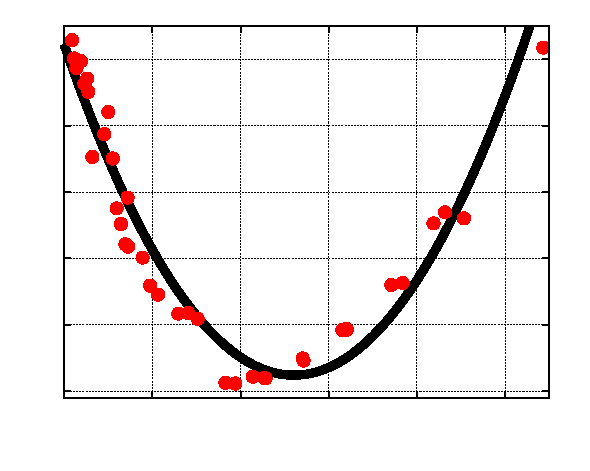
\includegraphics{PSPlainAverageDensity}}%
    \gplfronttext
  \end{picture}%
\endgroup

	\end{center}
	\caption[Zero-angle intensity of the PS-Plain particles.]{Intensity at zero-angle of the PS-Plain particles as a function of the solvent electron density measured with continuous contrast variation in SAXS. The minimum defines the average electron density of the particle.}
	\label{fig:PSPlainAverageDensity}
\end{figure}

The mass density of the particle can also be determined by this approach because the electron density is directly proportional to the mass density, as reviewed in chapter \ref{chap:theory_SAXS}. A PS-Plain density of ($1.043\pm0.003$) g cm$^{-3}$ is obtained, although an assumption about the polymer (or monomer) components and their atomic structure is necessary for the calculation. Therefore, a typical value of $Z/A=0.54$ was adopted for this conversion, where $Z$ and $A$ are the average atomic number and mass of the polymer respectively. This value is characteristic of polymers (or monomers) such as PS, PMMA or MMA, and very close to the $Z/A$ ratio of MAA (0.53), polyvynil chloride (0.51) or polyethylene (0.57).

The density uncertainty is associated to the vertical size of the focused X-ray beam as discussed in \ref{sec:SolventCalibration}, which typically corresponds to an associated uncertainty of 1 nm$^{-1}$ or a relative uncertainty of around 3 $\%$. Furthermore, the result can be affected by the polymeric composition of the colloid, and therefore, the assumption of $Z/A$, although an upper limit of 5 $\%$ is expected from this contribution.

\subsection{Mass density of the PS-Plain particles: Validation with DCS}

In figure \ref{fig:DensityComparison}, the value measured with the $I(0)$ approach from the continuous contrast variation experiment is compared to the average density of the PS-Plain colloid measured with different DCS configurations. For single disc setups, the size value used for the density calculation was 147 nm, as measured by single-contrast SAXS, while combining the information from the standard setup and the low density disc configuration allowed the measurement of the density independently of the particle diameter, as explained in section \ref{sec:interlab_size_comparison}.

The results agree with each other within their stated measurement uncertainties, although DCS measurements exhibit slightly higher densities than SAXS. Typical causes of systematic errors in DCS are the inaccuracy of the size and density of the calibration standard and the thermal variation in the centrifuge gradient during the measurements, which affect its viscosity and density \citep{kamiti_simultaneous_2012}. A temperature variation within the gradient of about 7 $^{\circ}$C before and after measurements was detected and a period of 30 min was considered appropriate to reach reliable thermal equilibrium. In the low density disc configuration, the accuracy of the average density of the D$_2$0 sucrose gradient becomes an important source of uncertainty.
\begin{figure}
	\begin{center}
		% GNUPLOT: LaTeX picture with Postscript
\begingroup
  \makeatletter
  \providecommand\color[2][]{%
    \GenericError{(gnuplot) \space\space\space\@spaces}{%
      Package color not loaded in conjunction with
      terminal option `colourtext'%
    }{See the gnuplot documentation for explanation.%
    }{Either use 'blacktext' in gnuplot or load the package
      color.sty in LaTeX.}%
    \renewcommand\color[2][]{}%
  }%
  \providecommand\includegraphics[2][]{%
    \GenericError{(gnuplot) \space\space\space\@spaces}{%
      Package graphicx or graphics not loaded%
    }{See the gnuplot documentation for explanation.%
    }{The gnuplot epslatex terminal needs graphicx.sty or graphics.sty.}%
    \renewcommand\includegraphics[2][]{}%
  }%
  \providecommand\rotatebox[2]{#2}%
  \@ifundefined{ifGPcolor}{%
    \newif\ifGPcolor
    \GPcolortrue
  }{}%
  \@ifundefined{ifGPblacktext}{%
    \newif\ifGPblacktext
    \GPblacktextfalse
  }{}%
  % define a \g@addto@macro without @ in the name:
  \let\gplgaddtomacro\g@addto@macro
  % define empty templates for all commands taking text:
  \gdef\gplbacktext{}%
  \gdef\gplfronttext{}%
  \makeatother
  \ifGPblacktext
    % no textcolor at all
    \def\colorrgb#1{}%
    \def\colorgray#1{}%
  \else
    % gray or color?
    \ifGPcolor
      \def\colorrgb#1{\color[rgb]{#1}}%
      \def\colorgray#1{\color[gray]{#1}}%
      \expandafter\def\csname LTw\endcsname{\color{white}}%
      \expandafter\def\csname LTb\endcsname{\color{black}}%
      \expandafter\def\csname LTa\endcsname{\color{black}}%
      \expandafter\def\csname LT0\endcsname{\color[rgb]{1,0,0}}%
      \expandafter\def\csname LT1\endcsname{\color[rgb]{0,1,0}}%
      \expandafter\def\csname LT2\endcsname{\color[rgb]{0,0,1}}%
      \expandafter\def\csname LT3\endcsname{\color[rgb]{1,0,1}}%
      \expandafter\def\csname LT4\endcsname{\color[rgb]{0,1,1}}%
      \expandafter\def\csname LT5\endcsname{\color[rgb]{1,1,0}}%
      \expandafter\def\csname LT6\endcsname{\color[rgb]{0,0,0}}%
      \expandafter\def\csname LT7\endcsname{\color[rgb]{1,0.3,0}}%
      \expandafter\def\csname LT8\endcsname{\color[rgb]{0.5,0.5,0.5}}%
    \else
      % gray
      \def\colorrgb#1{\color{black}}%
      \def\colorgray#1{\color[gray]{#1}}%
      \expandafter\def\csname LTw\endcsname{\color{white}}%
      \expandafter\def\csname LTb\endcsname{\color{black}}%
      \expandafter\def\csname LTa\endcsname{\color{black}}%
      \expandafter\def\csname LT0\endcsname{\color{black}}%
      \expandafter\def\csname LT1\endcsname{\color{black}}%
      \expandafter\def\csname LT2\endcsname{\color{black}}%
      \expandafter\def\csname LT3\endcsname{\color{black}}%
      \expandafter\def\csname LT4\endcsname{\color{black}}%
      \expandafter\def\csname LT5\endcsname{\color{black}}%
      \expandafter\def\csname LT6\endcsname{\color{black}}%
      \expandafter\def\csname LT7\endcsname{\color{black}}%
      \expandafter\def\csname LT8\endcsname{\color{black}}%
    \fi
  \fi
  \setlength{\unitlength}{0.0500bp}%
  \begin{picture}(5668.00,4534.00)%
    \gplgaddtomacro\gplbacktext{%
      \csname LTb\endcsname%
      \put(548,1409){\makebox(0,0)[r]{\strut{} 1.04}}%
      \csname LTb\endcsname%
      \put(548,1779){\makebox(0,0)[r]{\strut{} 1.05}}%
      \csname LTb\endcsname%
      \put(548,2150){\makebox(0,0)[r]{\strut{} 1.06}}%
      \csname LTb\endcsname%
      \put(548,2520){\makebox(0,0)[r]{\strut{} 1.07}}%
      \csname LTb\endcsname%
      \put(868,1092){\rotatebox{-45}{\makebox(0,0)[l]{\strut{}Normal Disc}}}%
      \csname LTb\endcsname%
      \put(1338,1092){\rotatebox{-45}{\makebox(0,0)[l]{\strut{}Combined}}}%
      \csname LTb\endcsname%
      \put(1809,1092){\rotatebox{-45}{\makebox(0,0)[l]{\strut{}Low Density}}}%
      \csname LTb\endcsname%
      \put(2279,1092){\rotatebox{-45}{\makebox(0,0)[l]{\strut{}SAXS}}}%
      \csname LTb\endcsname%
      \put(3220,1092){\rotatebox{-45}{\makebox(0,0)[l]{\strut{}DCS}}}%
      \csname LTb\endcsname%
      \put(3690,1092){\rotatebox{-45}{\makebox(0,0)[l]{\strut{}SAXS}}}%
      \csname LTb\endcsname%
      \put(4631,1092){\rotatebox{-45}{\makebox(0,0)[l]{\strut{}DCS}}}%
      \csname LTb\endcsname%
      \put(5101,1092){\rotatebox{-45}{\makebox(0,0)[l]{\strut{}SAXS}}}%
      \put(-222,2680){\rotatebox{-270}{\makebox(0,0){\strut{}Density / g cm$^{-3}$}}}%
    }%
    \gplgaddtomacro\gplfronttext{%
    }%
    \gplgaddtomacro\gplbacktext{%
      \csname LTb\endcsname%
      \put(548,3349){\makebox(0,0)[r]{\strut{} 1.17}}%
      \csname LTb\endcsname%
      \put(548,3846){\makebox(0,0)[r]{\strut{} 1.18}}%
      \colorrgb{0.00,0.00,1.00}%
      \put(1235,2952){\makebox(0,0)[l]{\strut{}\smaller PS-Plain}}%
      \put(3032,3051){\makebox(0,0)[l]{\strut{}\smaller PS-COOH}}%
      \put(4066,4243){\makebox(0,0)[l]{\strut{}\smaller PMMA-COOH}}%
    }%
    \gplgaddtomacro\gplfronttext{%
    }%
    \gplbacktext
    \put(0,0){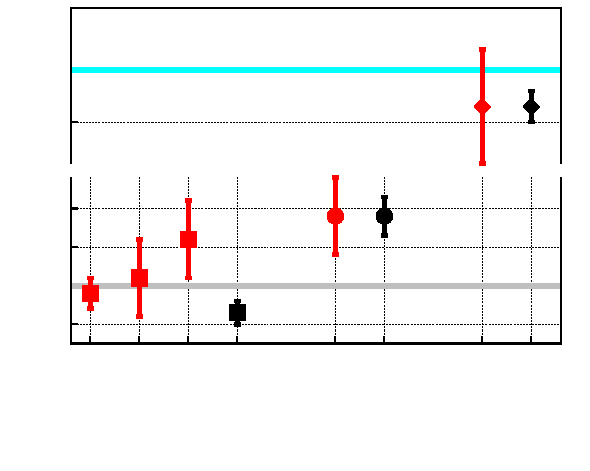
\includegraphics{DensityComparison}}%
    \gplfronttext
  \end{picture}%
\endgroup

	\end{center}
	\caption[Mass densities of 3 polymeric colloids measured with SAXS and DCS.]{Comparison between the mass densities of 3 polymeric colloids measured with SAXS using the $I(0)$ approach (black) and DCS (red): PS-Plain (squares), PS-COOH (circles) and PMMA-COOH (diamonds). The nominal densities of polystyrene (1.05 g cm$^{-3}$) and PMMA (1.18 g cm$^{-3}$) are also shown in the plot as horizontal lines \citep{dingenouts_analysis_1999}.}
	\label{fig:DensityComparison}
\end{figure}

\subsection{Density determination of heavier polymeric colloids}
The applicability of the continuous contrast variation techniques is further discussed by comparing with DCS for higher-density polymeric colloids, as summarized in figure \ref{fig:DensityComparison}. The density of the PS-COOH particles derived from the $I(0)$ approach is in excellent agreement with that measured by DCS using a standard configuration and assuming a particle diameter of 99.4 nm, which was obtained by SAXS. Considering the similar electronic composition of these polymers and the average electron density of the particle $\rho_0=346$ nm\(^{-3}\), an average mass density of the particles of ($1.068\pm0.005$) g cm$^{-3}$ can be calculated. These core-shell particles, more dense than polystyrene as detailed in section \ref{sec:coreshell_fit}, illustrate the tendency during the emulsion polymerization to segregate polar and nonpolar components \citep{dingenouts_structure_1994}.

Similarly, the density of the PMMA-COOH colloids was measured using the standard DCS setup and assuming a diameter of 186.5 nm, as measured by SAXS. This value is compared to the density of ($1.173\pm0.003$) g cm$^{-3}$ obtained by computing the intensity at zero-angle of a continuous contrast variation experiment. Again, both techniques are in excellent agreement and reveal a mass density slightly lower than the expected PMMA density of 1.18 g cm$^{-3}$ \citep{dingenouts_analysis_1999}.

This result highlights the fact that the density of polymeric colloids in suspension may vary from that of bulk materials, for example dry particles. For instance, a volume variation can be expected when going from the MMA monomer to the polymer PMMA \citep{nichols_prediction_1950} which might reduce the colloid density.
		
	
	\chapter{Continuous contrast variation applied to relevant bio-materials}
\label{chap:bio_applications}

The world of medicine has received very welcoming the new advances in nanoscience, as the application of nanoparticles in medicine opens the continuously growing field of nanomedicine. \cite{nie_nanotechnology_2007, sahoo_nanotech_2003, wickline_nanotechnology_2003, zhou_nano-enabled_2014, rosen_rise_2005}

The usage of lipid vesicles as nanocarriers for drug delivery has opened the continuously growing field of nanomedicine. 

The costs of health care are increasing rapidly throughout Europe due to ageing of the population. One of the instruments to reduce health care costs is early diagnosis of disease, which improves the efficacy of medical treatment.

nanoscience, if used to understand existing biological structures at the nanometer length scale, would potentially revolutionize several fields of biological science that are struggling with thechallenges of working at such small length scales

The tools of nanoscience and the key questions of lipoprotein biology are well matched. 



What is a liposome? Lipid vesicle (not explained in caelyx or in osmotic pressuer) Lipid vesicle formed with a phospholipid bilayer membrane and intraliposomal volume filled with buffer.


Liposomes, or lipid vesicles, have an increasing importance in the emerging field of nanomedicine. Their capacity to encapsulate hydrophillic compounds within the closed bilayer membrane opens exciting new possibilities in drug-delivery or as platforms for imaging agents.


The use of SAXS in liposome research is widespread. For instance, it has been applied to characterize the lamellarity, bilayer thickness, area per lipid ratio and the thickness of the PEG-layer of different liposomal samples, also to describe the influence of extrusion on the average number of bilayers and to determine the electron density profile of liposomes and biological vesicles.

Despite SAXS being a usual method of choice for the accurate size determination of nanomaterials, the interpretation of the scattering curves, i.e. the uniqueness of the solution of the model fitting, is frequently intricate for complex samples. Liposomal drugs belong to this class, as the inner structure of the phospholipid bilayer and the incorporated drug also contribute to the scattering intensity. 

In general, SAXS characterization of NPs with a broad size distribution, a heterogeneous composition or with a complicated inner structure require either a priori knowledge about the morphology of the sample or the measurement of complementary scattering curves obtained under different experimental conditions. 


Solvent contrast variation in SAXS belongs to the latter approach as it is based on the variation of the scattering curves caused by the addition of a suitable contrast agent to the suspending medium. 


\section{Materials and methods}

Caelyx (iodixanol and sucrose), Lipsomes (PEG and plain), Lipoproteins (HDL and LDL) , Protein coated particles (IgG + PS-COOH)


\subsection{Caelyx: PEGylated liposomal doxorubicin}
\label{sec:materials_caelyx}
The PEGylated liposomal formulation of doxorubicin, Caelyx $\textregistered$ (SP Europe, Brussels, Belgium), was purchased from Hungaropharma Ltd. Caelyx $\textregistered$ (or Doxil $\textregistered$ in US) consist of liposomes formed by fully hydrogenated soy phosphatydilcholine (HSPC), cholesterol, and DSPE-PEG2000 (N-(carbonyl-methoxypolyethylene glycol 2000)-1,2-distearoyl-sn-glycero-3-phosphoethanolamine). The latter results a steric barrier at the liposomal surface due to the PEG 2000 residues. Doxorubicin is encapsulated in Caelyx $\textregistered$ via an active loading procedure, which results a crystal-like doxorubicin precipitate inside the liposomes, as depicted schematically in figure 0. 

\begin{figure}
	\centering
		\subfloat[Cryo-TEM]{\resizebox{0.4\linewidth}{!}{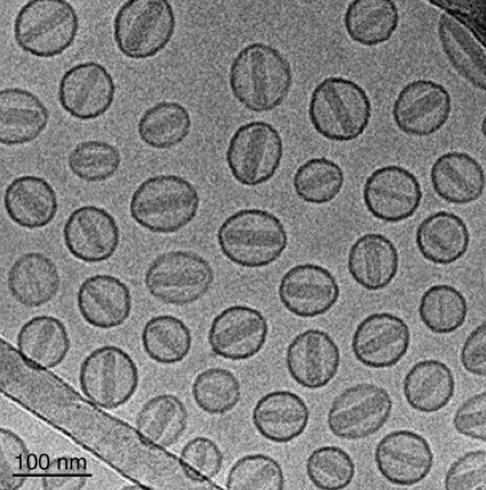
\includegraphics{Figures/CaelyxCryoTEM.png}}\label{fig:CaelyxCryoTEM}}
		\subfloat[Scheme]{\def\svgwidth{0.7\linewidth}{\input{Figures/CaelyxScheme.pdf_tex}}\label{fig:CaelyxScheme}}
		\caption{Cryo-TEM  of Caelyx $\textregistered$ \cite{barenholz_doxil_2012} and schematic representation of the PEGylated liposomal doxorubicin morphology.}
\end{figure}

The suspending medium contrast variation study was performed with the iso-osmolar contrast agent Optiprep $\textregistered$ (an aqueous solution of iodixanol), which has an osmolality of 290 to 310 mOsm kg$^{-1}$. The suspending medium density gradient was achieved by bringing together two mixtures of different densities: For the bottom of the capillary, a high density mixture of Caelyx $\textregistered$ was prepared with an Optiprep $\textregistered$ mass fraction of 35 $\%$ and a corresponding solvent electron density of 365.2 nm$^{-3}$, whilst on the top side of the capillary a low density preparation of Caelyx $\textregistered$  using phosphate buffered saline solution (pH 7.4) with the same volume fraction of Caelyx $\textregistered$ was introduced, with a solvent electron density of 341.9 nm$^{-3}$. By employing Optiprep $\textregistered$ as a contrast agent, the suspending medium osmolality is constant along the capillary. 

In order to study the effects of the suspending medium osmolality in the liposomal drug carrier, another capillary with a density gradient was created by introducing a dense aqueous sucrose solution with 37.8 $\%$ sucrose mass fraction (Sigma-Aldrich, Missouri, USA) at the bottom of the capillary (which corresponds to an electron density of 381.1 nm$^{-3}$ and a solvent osmolality of 1775.6 mOsm kg$^{-1}$), whereas a lighter solution was produced without sucrose by adding pure water to get the same Caelyx $\textregistered$ concentration. Considering the sucrose mass fraction of the Caelyx® buffer to be 10$\%$, this latter preparation has an electron density of 339.4 nm$^{-3}$ and an osmolality of 151.1 mOsm kg$^{-1}$. 

A wide-angle configuration was employed to observe the diffraction peak of the fiber-like doxorubicin precipitate encapsulated in the liposomes. At this configuration, the sample-to-detector distance was reduced to $L = (569 \pm  1)$ mm and as a result the available $q$-range was extended until 5.55 nm$^{-1}$. For the wide-angle X-ray scattering measurements, a density gradient capillary was prepared using a denser aqueous solution with a sucrose mass fraction of 34$\%$ and a lighter one with 6$\%$.

\begin{figure}
	\centering
		% GNUPLOT: LaTeX picture with Postscript
\begingroup
  \makeatletter
  \providecommand\color[2][]{%
    \GenericError{(gnuplot) \space\space\space\@spaces}{%
      Package color not loaded in conjunction with
      terminal option `colourtext'%
    }{See the gnuplot documentation for explanation.%
    }{Either use 'blacktext' in gnuplot or load the package
      color.sty in LaTeX.}%
    \renewcommand\color[2][]{}%
  }%
  \providecommand\includegraphics[2][]{%
    \GenericError{(gnuplot) \space\space\space\@spaces}{%
      Package graphicx or graphics not loaded%
    }{See the gnuplot documentation for explanation.%
    }{The gnuplot epslatex terminal needs graphicx.sty or graphics.sty.}%
    \renewcommand\includegraphics[2][]{}%
  }%
  \providecommand\rotatebox[2]{#2}%
  \@ifundefined{ifGPcolor}{%
    \newif\ifGPcolor
    \GPcolortrue
  }{}%
  \@ifundefined{ifGPblacktext}{%
    \newif\ifGPblacktext
    \GPblacktextfalse
  }{}%
  % define a \g@addto@macro without @ in the name:
  \let\gplgaddtomacro\g@addto@macro
  % define empty templates for all commands taking text:
  \gdef\gplbacktext{}%
  \gdef\gplfronttext{}%
  \makeatother
  \ifGPblacktext
    % no textcolor at all
    \def\colorrgb#1{}%
    \def\colorgray#1{}%
  \else
    % gray or color?
    \ifGPcolor
      \def\colorrgb#1{\color[rgb]{#1}}%
      \def\colorgray#1{\color[gray]{#1}}%
      \expandafter\def\csname LTw\endcsname{\color{white}}%
      \expandafter\def\csname LTb\endcsname{\color{black}}%
      \expandafter\def\csname LTa\endcsname{\color{black}}%
      \expandafter\def\csname LT0\endcsname{\color[rgb]{1,0,0}}%
      \expandafter\def\csname LT1\endcsname{\color[rgb]{0,1,0}}%
      \expandafter\def\csname LT2\endcsname{\color[rgb]{0,0,1}}%
      \expandafter\def\csname LT3\endcsname{\color[rgb]{1,0,1}}%
      \expandafter\def\csname LT4\endcsname{\color[rgb]{0,1,1}}%
      \expandafter\def\csname LT5\endcsname{\color[rgb]{1,1,0}}%
      \expandafter\def\csname LT6\endcsname{\color[rgb]{0,0,0}}%
      \expandafter\def\csname LT7\endcsname{\color[rgb]{1,0.3,0}}%
      \expandafter\def\csname LT8\endcsname{\color[rgb]{0.5,0.5,0.5}}%
    \else
      % gray
      \def\colorrgb#1{\color{black}}%
      \def\colorgray#1{\color[gray]{#1}}%
      \expandafter\def\csname LTw\endcsname{\color{white}}%
      \expandafter\def\csname LTb\endcsname{\color{black}}%
      \expandafter\def\csname LTa\endcsname{\color{black}}%
      \expandafter\def\csname LT0\endcsname{\color{black}}%
      \expandafter\def\csname LT1\endcsname{\color{black}}%
      \expandafter\def\csname LT2\endcsname{\color{black}}%
      \expandafter\def\csname LT3\endcsname{\color{black}}%
      \expandafter\def\csname LT4\endcsname{\color{black}}%
      \expandafter\def\csname LT5\endcsname{\color{black}}%
      \expandafter\def\csname LT6\endcsname{\color{black}}%
      \expandafter\def\csname LT7\endcsname{\color{black}}%
      \expandafter\def\csname LT8\endcsname{\color{black}}%
    \fi
  \fi
  \setlength{\unitlength}{0.0500bp}%
  \begin{picture}(5668.00,4534.00)%
    \gplgaddtomacro\gplbacktext{%
      \csname LTb\endcsname%
      \put(946,1162){\makebox(0,0)[r]{\strut{} 1}}%
      \put(946,2313){\makebox(0,0)[r]{\strut{} 10}}%
      \put(946,3464){\makebox(0,0)[r]{\strut{} 100}}%
      \put(2391,484){\makebox(0,0){\strut{} 0.1}}%
      \put(5271,484){\makebox(0,0){\strut{} 1}}%
      \put(176,2486){\rotatebox{-270}{\makebox(0,0){\strut{}Scattering Intensity / a.u.}}}%
      \put(3174,154){\makebox(0,0){\strut{}$q$ / nm$^{-1}$}}%
    }%
    \gplgaddtomacro\gplfronttext{%
      \csname LTb\endcsname%
      \put(4284,4096){\makebox(0,0)[r]{\strut{}Caelyx in buffer}}%
      \csname LTb\endcsname%
      \put(4284,3876){\makebox(0,0)[r]{\strut{}Caelyx in 9.1$\%$ iodixanol}}%
      \csname LTb\endcsname%
      \put(4284,3656){\makebox(0,0)[r]{\strut{}SSL in buffer}}%
      \csname LTb\endcsname%
      \put(4284,3436){\makebox(0,0)[r]{\strut{}Vesicle fit}}%
    }%
    \gplbacktext
    \put(0,0){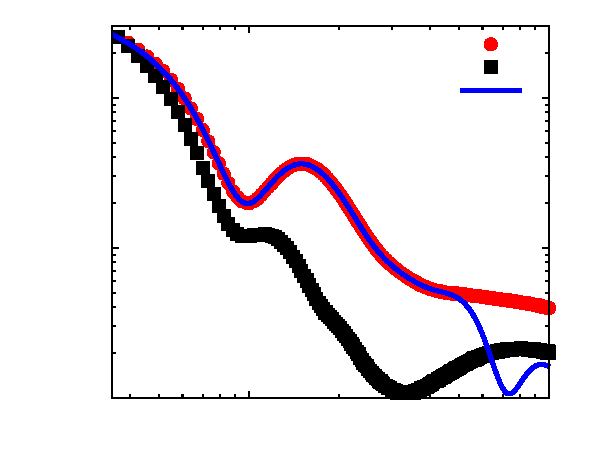
\includegraphics{CaelyxIodixanolSingleContrast}}%
    \gplfronttext
  \end{picture}%
\endgroup

		\caption{Caelyx in buffer and in 9.1 $\%$ iodixanol: SAXS scattering curve at single contrast compared to that of an SSL of similar size}
		\label{fig:CaelyxIodixanolSingleContrast}
\end{figure}

\subsection{Lipid vesicles: PEGylated and plain liposomes}
\label{sec:materials_liposome}

\textcolor{red}{DO WE KNOW THE ZETA-POTENTIAL????}

ACCORDING TO \cite{varga_osmotic_2014}

Synthetic high-purity hydrogenated soy lecithin (HSPC) and 1,2-distearoyl-sn-glycero-3-phosphoethanolamine-N-[methoxy (polyethylene glycol)-2000] (DSPE-PEG 2000) were purchased from NOF Corporation (Japan) and Avanti Polar Lipids (USA), respectively. Cholesterol was purchased from Sigma-Aldrich (Hungary). All of the chemicals were used without further purification. SSL samples were prepared by the hydration, freeze-thaw and extrusion method. Briefly, the components in the weight ratios of HSPC:DSPE-PEG 2000: cholesterol = 3:1:1 (corresponding to the molar ratios of 0.565:0.053:0.382) were dissolved in a chloroform:methanol mixture (2:1 v/v). The composition used is identical to that of the first commercially available liposomal drug, namely Doxil/Caelyx (US/EU). The solvent was then evaporated at 313 K and the resulting lipid film was kept under vacuum overnight to remove residual traces of the solvent. A 10 mM Tris pH 7.4 buffer solution (Sigma–Aldrich, Hungary) made with ultrapure water (18.2 M  cm) was added to the sample to obtain a total lipid concentration of 16 mg ml-1. Ten freeze-thaw cycles using liquid nitrogen and a lukewarm water bath were applied for homogenization. Finally, the samples were extruded ten times through 100 nm pore size polycarbonate filters (Nucleopore, Whatman Inc.) using a LIPEX extruder (Northern Lipids Inc., Canada). The extrusion was performed at 333 K.

The SSL samples were also made of HSPC. Their composition is:

HSPC: 9.6 mg/ml
cholesterol: 3.2 mg/ml
DSPE-PEG2k: 3.2 mg/ml

ratio 3:1:1 (HSPC:chol:PEG)

It is clear from the sizes and polydispersities obtained from the DLS measurements that the morphology of the liposomes is not easily reproducible. The tendency is that \textbf{plain liposomes show a higher polydispersity than SSLs.} It can also be said that \textbf{polydispersity increases with increasing pore size.} 

The deviations within the samples extruded with the same pore size (e.g. 80 nm pore) are suspicious. The extrusion pore sizes are 50, 80, 100, 200, 400

It must be considered also that PEG2k has an hydrodynamic radius of around 3 nm (REF) so \textbf{the PEG size should be subtracted from the overall DLS size} measured in order to obtain the liposome size.


\subsubsection{DLS size measurements}

DLS measurements were performed on a W130i apparatus (Avid Nano Ltd, High Wycombe, UK) and using a low-volume disposable cuvette (UVette, Eppendorf Austria GmbH). First, 70 ml of the liposome sample prepared in a salt-free buffer was measured ten times for 30 s. This was followed by addition of 70 ml of buffered saline solution (10 mM Tris pH 7.4, 0.3 M NaCl), and the sequence with 30 s measurements with ten repeats was started again. In a control measurement, the liposome sample was mixed with a salt-free buffer and the same procedure was repeated. 

\subsection{PS-COOH particles coated with IgG}

Polystyrene nanoparticles with carboxylated surfaces and a nominal diameter of 105 nm were purchased from Kisker Biotech (Steinfurt, Germany) \textcolor{red}{SAME PARTICLES, \cite{minelli_characterization_2014}}. A set of four IgG-coated polystyrene nanoparticle samples was prepared by incubating 0.05 $\%$ (w/w) particles with varying concentrations of IgG from 0.5 to 4 g L in 100 mM Tris buffer at pH 8 under continuous shaking for 2 h. Any unbound IgG was then removed from the particle samples by three cycles of centrifugation and redispersion in clean buffer. The use of 6 mM dithiothreitol (DTT) in IgG-coated particle samples was investigated. A sample of aggregated IgG-coated particles ($\rho$IgG = 0.5 g L ) was incubated in a 6 mM DTT solution for 115 min. An additional set of IgG-coated particles ($\rho$IgG = 2 g L ) was produced to study the effect of DTT by incubating them in a 6 mM DTT solution for 20 min and 24 h respectively.


NP Surface + 4 mg/mL IgG physisorbed at surface



\subsection{Lipoproteins}
HDL and LDL

Purchased from Merck Milipore, Merck KGaA, Darmstadt, Deutschland

in buffer: In 150 mM NaCl, 0.01$\%$ EDTA, pH 7.4. 

$>=$95$\%$ of total lipoprotein content by electrophoresis 

\subsubsection{Lipoprotein, High density (HDL)}
Native high density lipoproteins from human plasma. Cholesterol-carrier lipoprotein that acts as scavenger of tissue cholesterol. Important in cholesterol efflux from tissues. Involved in return of cholesterol from the periphery to the liver for removal as bile acids. Composition: 55-45$\%$ lipid, 45-55$\%$ protein.

A 10 mg vial contains ca. 5 mg of protein. 


437641 HDL D00163977 shelf life time 15/05/2015, protein concentration 14.29 mg/ml

\subsubsection{Lipoprotien, Low density (LDL)}

Native low density lipoproteins from human plasma. Cholesterol-carrier lipoprotein responsible for delivery of lipids (cholesterol) from liver to tissues. Composition: 78-81$\%$ lipid; 19-22$\%$ protein.

A 10 mg vial contains ca. 2 mg of protein.

437644 LDL D00164726 shelf life time 21/05/2015,
protein concentration 5.96 mg/ml

\begin{figure}
	\centering
		% GNUPLOT: LaTeX picture with Postscript
\begingroup
  \makeatletter
  \providecommand\color[2][]{%
    \GenericError{(gnuplot) \space\space\space\@spaces}{%
      Package color not loaded in conjunction with
      terminal option `colourtext'%
    }{See the gnuplot documentation for explanation.%
    }{Either use 'blacktext' in gnuplot or load the package
      color.sty in LaTeX.}%
    \renewcommand\color[2][]{}%
  }%
  \providecommand\includegraphics[2][]{%
    \GenericError{(gnuplot) \space\space\space\@spaces}{%
      Package graphicx or graphics not loaded%
    }{See the gnuplot documentation for explanation.%
    }{The gnuplot epslatex terminal needs graphicx.sty or graphics.sty.}%
    \renewcommand\includegraphics[2][]{}%
  }%
  \providecommand\rotatebox[2]{#2}%
  \@ifundefined{ifGPcolor}{%
    \newif\ifGPcolor
    \GPcolortrue
  }{}%
  \@ifundefined{ifGPblacktext}{%
    \newif\ifGPblacktext
    \GPblacktextfalse
  }{}%
  % define a \g@addto@macro without @ in the name:
  \let\gplgaddtomacro\g@addto@macro
  % define empty templates for all commands taking text:
  \gdef\gplbacktext{}%
  \gdef\gplfronttext{}%
  \makeatother
  \ifGPblacktext
    % no textcolor at all
    \def\colorrgb#1{}%
    \def\colorgray#1{}%
  \else
    % gray or color?
    \ifGPcolor
      \def\colorrgb#1{\color[rgb]{#1}}%
      \def\colorgray#1{\color[gray]{#1}}%
      \expandafter\def\csname LTw\endcsname{\color{white}}%
      \expandafter\def\csname LTb\endcsname{\color{black}}%
      \expandafter\def\csname LTa\endcsname{\color{black}}%
      \expandafter\def\csname LT0\endcsname{\color[rgb]{1,0,0}}%
      \expandafter\def\csname LT1\endcsname{\color[rgb]{0,1,0}}%
      \expandafter\def\csname LT2\endcsname{\color[rgb]{0,0,1}}%
      \expandafter\def\csname LT3\endcsname{\color[rgb]{1,0,1}}%
      \expandafter\def\csname LT4\endcsname{\color[rgb]{0,1,1}}%
      \expandafter\def\csname LT5\endcsname{\color[rgb]{1,1,0}}%
      \expandafter\def\csname LT6\endcsname{\color[rgb]{0,0,0}}%
      \expandafter\def\csname LT7\endcsname{\color[rgb]{1,0.3,0}}%
      \expandafter\def\csname LT8\endcsname{\color[rgb]{0.5,0.5,0.5}}%
    \else
      % gray
      \def\colorrgb#1{\color{black}}%
      \def\colorgray#1{\color[gray]{#1}}%
      \expandafter\def\csname LTw\endcsname{\color{white}}%
      \expandafter\def\csname LTb\endcsname{\color{black}}%
      \expandafter\def\csname LTa\endcsname{\color{black}}%
      \expandafter\def\csname LT0\endcsname{\color{black}}%
      \expandafter\def\csname LT1\endcsname{\color{black}}%
      \expandafter\def\csname LT2\endcsname{\color{black}}%
      \expandafter\def\csname LT3\endcsname{\color{black}}%
      \expandafter\def\csname LT4\endcsname{\color{black}}%
      \expandafter\def\csname LT5\endcsname{\color{black}}%
      \expandafter\def\csname LT6\endcsname{\color{black}}%
      \expandafter\def\csname LT7\endcsname{\color{black}}%
      \expandafter\def\csname LT8\endcsname{\color{black}}%
    \fi
  \fi
    \setlength{\unitlength}{0.0500bp}%
    \ifx\gptboxheight\undefined%
      \newlength{\gptboxheight}%
      \newlength{\gptboxwidth}%
      \newsavebox{\gptboxtext}%
    \fi%
    \setlength{\fboxrule}{0.5pt}%
    \setlength{\fboxsep}{1pt}%
\begin{picture}(5668.00,4534.00)%
    \gplgaddtomacro\gplbacktext{%
      \csname LTb\endcsname%
      \put(594,1164){\makebox(0,0)[r]{\strut{}$1$}}%
      \csname LTb\endcsname%
      \put(594,2489){\makebox(0,0)[r]{\strut{}$10$}}%
      \csname LTb\endcsname%
      \put(594,3815){\makebox(0,0)[r]{\strut{}$100$}}%
      \csname LTb\endcsname%
      \put(1074,484){\makebox(0,0){\strut{}$0.3$}}%
      \csname LTb\endcsname%
      \put(1743,484){\makebox(0,0){\strut{}$0.5$}}%
      \csname LTb\endcsname%
      \put(2650,484){\makebox(0,0){\strut{}$1$}}%
      \csname LTb\endcsname%
      \put(4089,484){\makebox(0,0){\strut{}$3$}}%
      \csname LTb\endcsname%
      \put(4758,484){\makebox(0,0){\strut{}$5$}}%
    }%
    \gplgaddtomacro\gplfronttext{%
      \csname LTb\endcsname%
      \put(220,2486){\rotatebox{-270}{\makebox(0,0){\strut{}Scattering Intensity / a.u.}}}%
      \put(2998,154){\makebox(0,0){\strut{}$q$ / nm$^{-1}$}}%
      \csname LTb\endcsname%
      \put(4284,4096){\makebox(0,0)[r]{\strut{}Experimental}}%
      \csname LTb\endcsname%
      \put(4284,3876){\makebox(0,0)[r]{\strut{}Model Fit}}%
    }%
    \gplbacktext
    \put(0,0){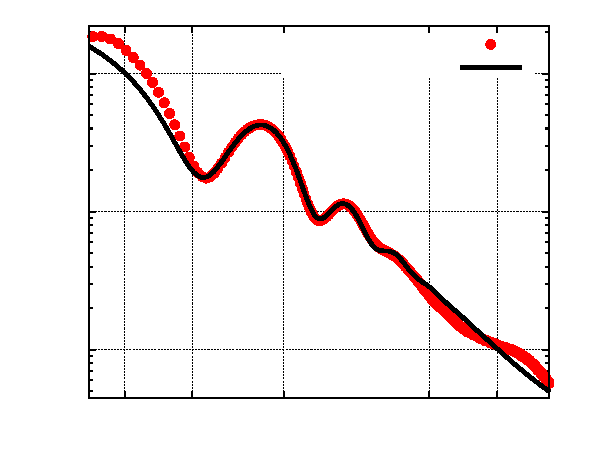
\includegraphics{HDLCoreShellFit}}%
    \gplfronttext
  \end{picture}%
\endgroup

		\caption{Scattering curve of HDL with subtracted background measured the 23.May2014. A simple core-shell model is fitted to the data: R=4.84, sigma=0.097,mu=-0.238, nu	=0.86, alpha=1.3}
		\label{fig:HDLCoreShellFit}
\end{figure}

\section{Traceable size determination of a liposomal drug}
\label{sec:caelyx_size}

The first approved nano-drug was Doxil$\textregistered$ (Caelyx$\textregistered$ in Europe), a PEGylated liposomal formulation of doxorubicin, which was followed by a few other products\cite{yeh_clinical_2011,barenholz_doxil_2012}. Nowadays there are approximately 250 nanomedicine products that are either approved by the relevant health agencies or are under clinical trials \cite{etheridge_big_2013}. On the other hand, there is a translational gap between the experimental work devoted to the development of new nano-drug candidates and the clinical realization of their use, which is also reflected in the high number of studies dealing with nanomedicine and the number of approved products on the market \cite{khorasani_closing_2014, venditto_cancer_2013}. As highlighted in a recent review by \cite{khorasani_closing_2014}, one of the main reasons for this translational gap is that the current characterization techniques possess limitations and there is a need for standardization on this field.

Among many relevant physicochemical properties of nano-drugs, one of the most important to be accurately determined is the size of the nanocarriers, which directly relates to the in vivo biodistribution of the drug. The ultimate goal in this regard is to reach a "traceable size determination" of the nanomaterial, which means that the measurand can be related to the SI unit "meter" through an unbroken chain of comparisons with known uncertainties. 

The most widely used technique for size determination in the field of nanomedicine is dynamic light scattering (DLS), which measures the hydrodynamic diameter of the nanoparticles (NPs) \cite{murphy_static_1997, hallett_vesicle_1991, egelhaaf_determination_1996, takahashi_precise_2008, jans_dynamic_2009, hoo_comparison_2008}. DLS is well-established and has indisputable advantages in the size characterization of the NPs, e.g. easy-to-use instrumentations, fast and low-cost operation, but it is not capable of a traceable size determination as there is no general relationship between the hydrodynamic diameter and the physical size of the NPs \cite{meli_traceable_2012}. 

Transmission electron microscopy (TEM) is also frequently used for sizing of NPs and proved to be an appropriate technique for solid nanoparticles, whilst its employment in soft matter NPs (e.g. liposomes, micelles and polymeric nanoparticles) is questionable due to the possible distortion of the particles during the drying process.  Although cryo-TEM could overcome this limitation \cite{li_doxorubicin_1998}, the statistical accuracy of this non-ensemble method is usually not sufficient.

SAXS is capable of traceable size determination for sufficiently monodisperse nanoparticles \cite{meli_traceable_2012} and therefore the continuous contrast variation technique with SAXS is a suitable method to assess the size of a complex liposomal drug, such as the PEGylated liposomal formulation of doxorubicin. The need of an iso-osmolal suspending medium to mimic the phyisiological conditions of plasma requires the use of Optiprep $\textregistered$ as contrast agent, as explained in section \ref{sec:materials_caelyx}.
 
SAXS curves of the liposomal doxorubicin sample measured at different suspending medium electron densities are shown in figure \ref{fig:CaelyxIodixanolContinuousSAXS}. In the scattering curves, it is possible to observe the variation of the curve features through the increase of the suspending medium density, which indicates the complexity of the internal structure of the nanocarrier. Besides, the appearance of an intersection point around $q = 0.12$ nm$^{-1}$ is a further indicator of the structural complexity of the drug-carrier.

\begin{figure}
	\centering
		\subfloat[Contrast variation with density gradient]{\resizebox{0.44\linewidth}{!}{% GNUPLOT: LaTeX picture with Postscript
\begingroup
  \makeatletter
  \providecommand\color[2][]{%
    \GenericError{(gnuplot) \space\space\space\@spaces}{%
      Package color not loaded in conjunction with
      terminal option `colourtext'%
    }{See the gnuplot documentation for explanation.%
    }{Either use 'blacktext' in gnuplot or load the package
      color.sty in LaTeX.}%
    \renewcommand\color[2][]{}%
  }%
  \providecommand\includegraphics[2][]{%
    \GenericError{(gnuplot) \space\space\space\@spaces}{%
      Package graphicx or graphics not loaded%
    }{See the gnuplot documentation for explanation.%
    }{The gnuplot epslatex terminal needs graphicx.sty or graphics.sty.}%
    \renewcommand\includegraphics[2][]{}%
  }%
  \providecommand\rotatebox[2]{#2}%
  \@ifundefined{ifGPcolor}{%
    \newif\ifGPcolor
    \GPcolortrue
  }{}%
  \@ifundefined{ifGPblacktext}{%
    \newif\ifGPblacktext
    \GPblacktextfalse
  }{}%
  % define a \g@addto@macro without @ in the name:
  \let\gplgaddtomacro\g@addto@macro
  % define empty templates for all commands taking text:
  \gdef\gplbacktext{}%
  \gdef\gplfronttext{}%
  \makeatother
  \ifGPblacktext
    % no textcolor at all
    \def\colorrgb#1{}%
    \def\colorgray#1{}%
  \else
    % gray or color?
    \ifGPcolor
      \def\colorrgb#1{\color[rgb]{#1}}%
      \def\colorgray#1{\color[gray]{#1}}%
      \expandafter\def\csname LTw\endcsname{\color{white}}%
      \expandafter\def\csname LTb\endcsname{\color{black}}%
      \expandafter\def\csname LTa\endcsname{\color{black}}%
      \expandafter\def\csname LT0\endcsname{\color[rgb]{1,0,0}}%
      \expandafter\def\csname LT1\endcsname{\color[rgb]{0,1,0}}%
      \expandafter\def\csname LT2\endcsname{\color[rgb]{0,0,1}}%
      \expandafter\def\csname LT3\endcsname{\color[rgb]{1,0,1}}%
      \expandafter\def\csname LT4\endcsname{\color[rgb]{0,1,1}}%
      \expandafter\def\csname LT5\endcsname{\color[rgb]{1,1,0}}%
      \expandafter\def\csname LT6\endcsname{\color[rgb]{0,0,0}}%
      \expandafter\def\csname LT7\endcsname{\color[rgb]{1,0.3,0}}%
      \expandafter\def\csname LT8\endcsname{\color[rgb]{0.5,0.5,0.5}}%
    \else
      % gray
      \def\colorrgb#1{\color{black}}%
      \def\colorgray#1{\color[gray]{#1}}%
      \expandafter\def\csname LTw\endcsname{\color{white}}%
      \expandafter\def\csname LTb\endcsname{\color{black}}%
      \expandafter\def\csname LTa\endcsname{\color{black}}%
      \expandafter\def\csname LT0\endcsname{\color{black}}%
      \expandafter\def\csname LT1\endcsname{\color{black}}%
      \expandafter\def\csname LT2\endcsname{\color{black}}%
      \expandafter\def\csname LT3\endcsname{\color{black}}%
      \expandafter\def\csname LT4\endcsname{\color{black}}%
      \expandafter\def\csname LT5\endcsname{\color{black}}%
      \expandafter\def\csname LT6\endcsname{\color{black}}%
      \expandafter\def\csname LT7\endcsname{\color{black}}%
      \expandafter\def\csname LT8\endcsname{\color{black}}%
    \fi
  \fi
    \setlength{\unitlength}{0.0500bp}%
    \ifx\gptboxheight\undefined%
      \newlength{\gptboxheight}%
      \newlength{\gptboxwidth}%
      \newsavebox{\gptboxtext}%
    \fi%
    \setlength{\fboxrule}{0.5pt}%
    \setlength{\fboxsep}{1pt}%
\begin{picture}(5668.00,4534.00)%
    \gplgaddtomacro\gplbacktext{%
      \csname LTb\endcsname%
      \put(814,1234){\makebox(0,0)[r]{\strut{}$0.01$}}%
      \csname LTb\endcsname%
      \put(814,1993){\makebox(0,0)[r]{\strut{}$0.1$}}%
      \csname LTb\endcsname%
      \put(814,2752){\makebox(0,0)[r]{\strut{}$1$}}%
      \csname LTb\endcsname%
      \put(814,3510){\makebox(0,0)[r]{\strut{}$10$}}%
      \csname LTb\endcsname%
      \put(814,4269){\makebox(0,0)[r]{\strut{}$100$}}%
      \csname LTb\endcsname%
      \put(1453,484){\makebox(0,0){\strut{}$0.05$}}%
      \csname LTb\endcsname%
      \put(2142,484){\makebox(0,0){\strut{}$0.1$}}%
      \csname LTb\endcsname%
      \put(2830,484){\makebox(0,0){\strut{}$0.2$}}%
      \csname LTb\endcsname%
      \put(3741,484){\makebox(0,0){\strut{}$0.5$}}%
      \csname LTb\endcsname%
      \put(4429,484){\makebox(0,0){\strut{}$1$}}%
    }%
    \gplgaddtomacro\gplfronttext{%
      \csname LTb\endcsname%
      \put(176,2266){\rotatebox{-270}{\makebox(0,0){\strut{}Scattering Intensity / cm$^{-1}$}}}%
      \put(2687,154){\makebox(0,0){\strut{}$q$ / nm$^{-1}$}}%
      \csname LTb\endcsname%
      \put(4691,1149){\makebox(0,0)[l]{\strut{}\smaller 345}}%
      \put(4691,1892){\makebox(0,0)[l]{\strut{}\smaller 350}}%
      \put(4691,2635){\makebox(0,0)[l]{\strut{}\smaller 355}}%
      \put(4691,3377){\makebox(0,0)[l]{\strut{}\smaller 360}}%
      \put(4691,4120){\makebox(0,0)[l]{\strut{}\smaller 365}}%
      \put(5351,2486){\rotatebox{-90}{\makebox(0,0){\strut{}\smaller Solvent Electron Density / nm$^{-3}$}}}%
    }%
    \gplbacktext
    \put(0,0){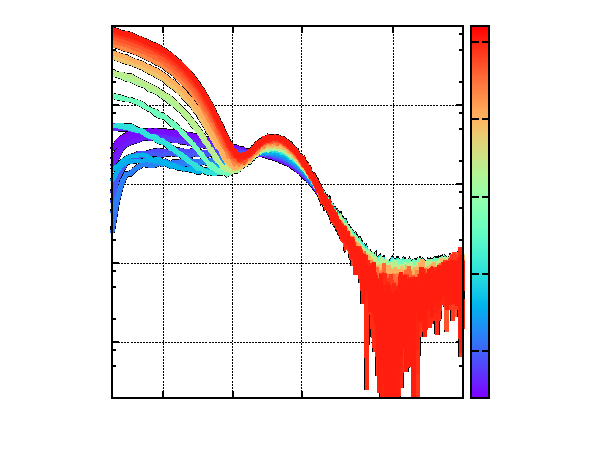
\includegraphics{CaelyxIodixanolContinuousSAXS}}%
    \gplfronttext
  \end{picture}%
\endgroup
}\label{fig:CaelyxIodixanolContinuousSAXS}}
		\subfloat[Isoscattering point positions]{\resizebox{0.44\linewidth}{!}{% GNUPLOT: LaTeX picture with Postscript
\begingroup
  \makeatletter
  \providecommand\color[2][]{%
    \GenericError{(gnuplot) \space\space\space\@spaces}{%
      Package color not loaded in conjunction with
      terminal option `colourtext'%
    }{See the gnuplot documentation for explanation.%
    }{Either use 'blacktext' in gnuplot or load the package
      color.sty in LaTeX.}%
    \renewcommand\color[2][]{}%
  }%
  \providecommand\includegraphics[2][]{%
    \GenericError{(gnuplot) \space\space\space\@spaces}{%
      Package graphicx or graphics not loaded%
    }{See the gnuplot documentation for explanation.%
    }{The gnuplot epslatex terminal needs graphicx.sty or graphics.sty.}%
    \renewcommand\includegraphics[2][]{}%
  }%
  \providecommand\rotatebox[2]{#2}%
  \@ifundefined{ifGPcolor}{%
    \newif\ifGPcolor
    \GPcolortrue
  }{}%
  \@ifundefined{ifGPblacktext}{%
    \newif\ifGPblacktext
    \GPblacktextfalse
  }{}%
  % define a \g@addto@macro without @ in the name:
  \let\gplgaddtomacro\g@addto@macro
  % define empty templates for all commands taking text:
  \gdef\gplbacktext{}%
  \gdef\gplfronttext{}%
  \makeatother
  \ifGPblacktext
    % no textcolor at all
    \def\colorrgb#1{}%
    \def\colorgray#1{}%
  \else
    % gray or color?
    \ifGPcolor
      \def\colorrgb#1{\color[rgb]{#1}}%
      \def\colorgray#1{\color[gray]{#1}}%
      \expandafter\def\csname LTw\endcsname{\color{white}}%
      \expandafter\def\csname LTb\endcsname{\color{black}}%
      \expandafter\def\csname LTa\endcsname{\color{black}}%
      \expandafter\def\csname LT0\endcsname{\color[rgb]{1,0,0}}%
      \expandafter\def\csname LT1\endcsname{\color[rgb]{0,1,0}}%
      \expandafter\def\csname LT2\endcsname{\color[rgb]{0,0,1}}%
      \expandafter\def\csname LT3\endcsname{\color[rgb]{1,0,1}}%
      \expandafter\def\csname LT4\endcsname{\color[rgb]{0,1,1}}%
      \expandafter\def\csname LT5\endcsname{\color[rgb]{1,1,0}}%
      \expandafter\def\csname LT6\endcsname{\color[rgb]{0,0,0}}%
      \expandafter\def\csname LT7\endcsname{\color[rgb]{1,0.3,0}}%
      \expandafter\def\csname LT8\endcsname{\color[rgb]{0.5,0.5,0.5}}%
    \else
      % gray
      \def\colorrgb#1{\color{black}}%
      \def\colorgray#1{\color[gray]{#1}}%
      \expandafter\def\csname LTw\endcsname{\color{white}}%
      \expandafter\def\csname LTb\endcsname{\color{black}}%
      \expandafter\def\csname LTa\endcsname{\color{black}}%
      \expandafter\def\csname LT0\endcsname{\color{black}}%
      \expandafter\def\csname LT1\endcsname{\color{black}}%
      \expandafter\def\csname LT2\endcsname{\color{black}}%
      \expandafter\def\csname LT3\endcsname{\color{black}}%
      \expandafter\def\csname LT4\endcsname{\color{black}}%
      \expandafter\def\csname LT5\endcsname{\color{black}}%
      \expandafter\def\csname LT6\endcsname{\color{black}}%
      \expandafter\def\csname LT7\endcsname{\color{black}}%
      \expandafter\def\csname LT8\endcsname{\color{black}}%
    \fi
  \fi
  \setlength{\unitlength}{0.0500bp}%
  \begin{picture}(5668.00,4534.00)%
    \gplgaddtomacro\gplbacktext{%
      \csname LTb\endcsname%
      \put(814,2055){\makebox(0,0)[r]{\strut{} 0.1}}%
      \csname LTb\endcsname%
      \put(814,3987){\makebox(0,0)[r]{\strut{} 1}}%
      \csname LTb\endcsname%
      \put(946,484){\makebox(0,0){\strut{} 0.05}}%
      \csname LTb\endcsname%
      \put(1947,484){\makebox(0,0){\strut{} 0.1}}%
      \csname LTb\endcsname%
      \put(2947,484){\makebox(0,0){\strut{} 0.2}}%
      \csname LTb\endcsname%
      \put(4270,484){\makebox(0,0){\strut{} 0.5}}%
      \csname LTb\endcsname%
      \put(5271,484){\makebox(0,0){\strut{} 1}}%
      \put(176,2266){\rotatebox{-270}{\makebox(0,0){\strut{}Rel. Std. Deviation}}}%
      \put(3108,154){\makebox(0,0){\strut{}$q$ / nm$^{-1}$}}%
    }%
    \gplgaddtomacro\gplfronttext{%
      \csname LTb\endcsname%
      \put(4548,4041){\makebox(0,0)[r]{\strut{}\smaller Background subtracted}}%
      \csname LTb\endcsname%
      \put(4548,3711){\makebox(0,0)[r]{\strut{}\smaller Raw data}}%
    }%
    \gplbacktext
    \put(0,0){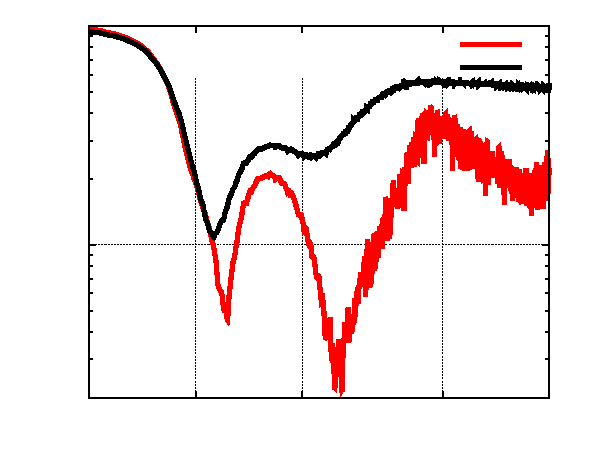
\includegraphics{CaelyxIodixanolIsopoint}}%
    \gplfronttext
  \end{picture}%
\endgroup
}\label{fig:CaelyxIodixanolIsopoint}}
		\caption{ a) Scattering curves at different suspending medium electron densities obtained with a solvent density gradient of Caelyx in aqueous iodixanol with constant buffer osmolality. Figure b) shows the precise position of the isoscattering points before and after the proper correction of the backbround.}
\end{figure}

The solvent background has been subtracted by measuring the scattering curves of a density gradient of Optiprep$\textregistered$ and buffer without nanocarriers. The low scattering power of the PEGylated liposomal doxorubicin at high $q$ values and the contribution of the iodixanol background result in an increased uncertainty in the high-$q$ range of the corrected scattering curves, although in the Fourier region below $q = 0.3$ nm$^{-1}$ the background effect is much less dominant.

\subsection{Isoscattering point approach}
In the low $q$ part of the scattering curve, an isoscattering point is clearly visible as highlighted in figure \ref{fig:CaelyxIodixanolContinuousSAXS}, where all the scattering curves intersect at one point. The isoscattering point position relates directly to the external radius of the measured particle inaccessible to the solvent, as explained in the \textcolor{red}{Supplementary Information.  WHERE?}. Therefore, the PEG-chains attached to the liposome surface might not be quantified in this approach due to the permeability of the polymer layer. The isoscattering point position is precisely determined by calculating the relative standard deviation of all the scattering curves at each $q$-value, as shown in figure \ref{fig:CaelyxIodixanolIsopoint}. \textcolor{blue}{As discussed before \textcolor{red}{WHERE????}, the proper subtraction of the solvent background is essential for the right interpretation of the data, specially for intense incoherent scatterers like Optiprep $\textregistered$. A clear shift in the minima of the relative standard deviation curve is observed in figure \ref{fig:CaelyxIodixanolIsopoint} after correcting the background effects.} Hence, the first isoscattering point $q^{\star}_1$ is located at $q^{\star}_1 = 0.123$ nm$^{-1}$, which corresponds to a radius of $R = 36.5$ nm and a diameter of 73 nm. A second isoscattering point at $q^{\star}_2 = 0.25$ nm$^{-1}$ is still visible, although the diffuseness of the isoscattering points at higher $q$ values, related with the polydispersity of the ensemble, makes it less reliable for the determination of the outer radius.

The determination of the $q$ values have an associated relative uncertainty of 0.1 $\%$, which corresponds to a size uncertainty of 0.6 nm. Furthermore, the radial integration of the scattering pattern was performed choosing a $q$-bin of size 0.0015 nm$^{-1}$, with an associated uncertainty in the size of 0.9 nm. Without further considerations, the Caelyx$\textregistered$ size uncertainty associated to the determination of the $q$-value of the isoscattering point is 1.1 nm. Other possible sources of uncertainty arise from the polydispersity degree of the sample and the ellipticity of the doxorubicin loaded liposomes, which might shift the measured position of the isoscattering point, although the uncertainty associated to them cannot be easily quantified. 

\subsection{Shape factor calculation}
In order to provide a traceable uncertainty for the obtained size value, we have used an alternative evaluation procedure, namely the calculation of the so-called shape factor which extracts all contributions from the 30 measured scattering curves that change with the contrast at different solvent densities. The shape factor of the Caelyx$\textregistered$ sample contains essentially information only about the shape and size distribution of the space filled up by the liposomes, i.e. the contributions of the phospholipid bilayer and the encapsulated doxorubicin to the scattering intensity are cancelled.  Thus, the complex interpretation of the original SAXS curve of Caelyx$\textregistered$ is avoided and enables the size determination of the liposomal carrier by fitting a simple analytical model for homogeneous spherical objects. A model with a certain ellipticity was also attempted, due to the slight liposomal eccentricity observed in TEM images though the best fit was accomplished with a spherical model. Details on the calculation of the shape factor as well as the analytical expression for the model fitting can be found in the \textcolor{red}{Supplementary Information.  WHERE?}. 

\begin{figure}
	\centering
		% GNUPLOT: LaTeX picture with Postscript
\begingroup
  \makeatletter
  \providecommand\color[2][]{%
    \GenericError{(gnuplot) \space\space\space\@spaces}{%
      Package color not loaded in conjunction with
      terminal option `colourtext'%
    }{See the gnuplot documentation for explanation.%
    }{Either use 'blacktext' in gnuplot or load the package
      color.sty in LaTeX.}%
    \renewcommand\color[2][]{}%
  }%
  \providecommand\includegraphics[2][]{%
    \GenericError{(gnuplot) \space\space\space\@spaces}{%
      Package graphicx or graphics not loaded%
    }{See the gnuplot documentation for explanation.%
    }{The gnuplot epslatex terminal needs graphicx.sty or graphics.sty.}%
    \renewcommand\includegraphics[2][]{}%
  }%
  \providecommand\rotatebox[2]{#2}%
  \@ifundefined{ifGPcolor}{%
    \newif\ifGPcolor
    \GPcolortrue
  }{}%
  \@ifundefined{ifGPblacktext}{%
    \newif\ifGPblacktext
    \GPblacktextfalse
  }{}%
  % define a \g@addto@macro without @ in the name:
  \let\gplgaddtomacro\g@addto@macro
  % define empty templates for all commands taking text:
  \gdef\gplbacktext{}%
  \gdef\gplfronttext{}%
  \makeatother
  \ifGPblacktext
    % no textcolor at all
    \def\colorrgb#1{}%
    \def\colorgray#1{}%
  \else
    % gray or color?
    \ifGPcolor
      \def\colorrgb#1{\color[rgb]{#1}}%
      \def\colorgray#1{\color[gray]{#1}}%
      \expandafter\def\csname LTw\endcsname{\color{white}}%
      \expandafter\def\csname LTb\endcsname{\color{black}}%
      \expandafter\def\csname LTa\endcsname{\color{black}}%
      \expandafter\def\csname LT0\endcsname{\color[rgb]{1,0,0}}%
      \expandafter\def\csname LT1\endcsname{\color[rgb]{0,1,0}}%
      \expandafter\def\csname LT2\endcsname{\color[rgb]{0,0,1}}%
      \expandafter\def\csname LT3\endcsname{\color[rgb]{1,0,1}}%
      \expandafter\def\csname LT4\endcsname{\color[rgb]{0,1,1}}%
      \expandafter\def\csname LT5\endcsname{\color[rgb]{1,1,0}}%
      \expandafter\def\csname LT6\endcsname{\color[rgb]{0,0,0}}%
      \expandafter\def\csname LT7\endcsname{\color[rgb]{1,0.3,0}}%
      \expandafter\def\csname LT8\endcsname{\color[rgb]{0.5,0.5,0.5}}%
    \else
      % gray
      \def\colorrgb#1{\color{black}}%
      \def\colorgray#1{\color[gray]{#1}}%
      \expandafter\def\csname LTw\endcsname{\color{white}}%
      \expandafter\def\csname LTb\endcsname{\color{black}}%
      \expandafter\def\csname LTa\endcsname{\color{black}}%
      \expandafter\def\csname LT0\endcsname{\color{black}}%
      \expandafter\def\csname LT1\endcsname{\color{black}}%
      \expandafter\def\csname LT2\endcsname{\color{black}}%
      \expandafter\def\csname LT3\endcsname{\color{black}}%
      \expandafter\def\csname LT4\endcsname{\color{black}}%
      \expandafter\def\csname LT5\endcsname{\color{black}}%
      \expandafter\def\csname LT6\endcsname{\color{black}}%
      \expandafter\def\csname LT7\endcsname{\color{black}}%
      \expandafter\def\csname LT8\endcsname{\color{black}}%
    \fi
  \fi
  \setlength{\unitlength}{0.0500bp}%
  \begin{picture}(5668.00,4534.00)%
    \gplgaddtomacro\gplbacktext{%
      \csname LTb\endcsname%
      \put(990,704){\makebox(0,0)[r]{\strut{} 1}}%
      \csname LTb\endcsname%
      \put(990,1595){\makebox(0,0)[r]{\strut{} 10}}%
      \csname LTb\endcsname%
      \put(990,2487){\makebox(0,0)[r]{\strut{} 100}}%
      \csname LTb\endcsname%
      \put(990,3378){\makebox(0,0)[r]{\strut{} 1000}}%
      \csname LTb\endcsname%
      \put(990,4269){\makebox(0,0)[r]{\strut{} 10000}}%
      \csname LTb\endcsname%
      \put(2279,484){\makebox(0,0){\strut{} 0.05}}%
      \csname LTb\endcsname%
      \put(3437,484){\makebox(0,0){\strut{} 0.1}}%
      \csname LTb\endcsname%
      \put(4594,484){\makebox(0,0){\strut{} 0.2}}%
      \csname LTb\endcsname%
      \put(5271,484){\makebox(0,0){\strut{} 0.3}}%
      \put(220,2486){\rotatebox{-270}{\makebox(0,0){\strut{}Shape Factor / a.u.}}}%
      \put(3196,154){\makebox(0,0){\strut{}$q$ / nm$^{-1}$}}%
    }%
    \gplgaddtomacro\gplfronttext{%
      \csname LTb\endcsname%
      \put(4284,4010){\makebox(0,0)[r]{\strut{}Experimental Data}}%
      \csname LTb\endcsname%
      \put(4284,3617){\makebox(0,0)[r]{\strut{}Sphere Fit}}%
    }%
    \gplbacktext
    \put(0,0){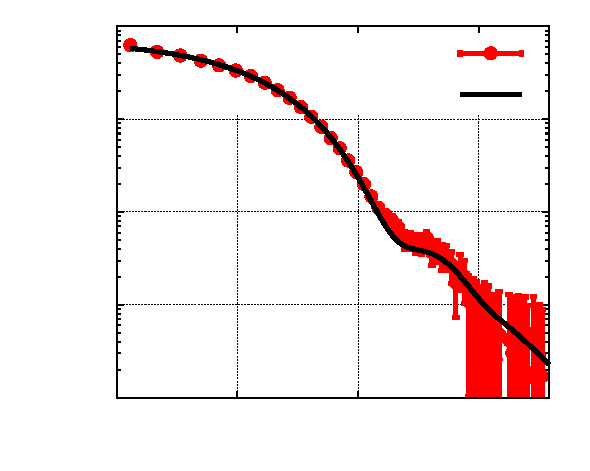
\includegraphics{CaelyxIodixanolResonantTerm}}%
    \gplfronttext
  \end{picture}%
\endgroup

		\caption{Expeirmental shape factor of the liposomes is shown with symbols and the model fit for homogeneous spherical particles is depicted with a thick line.}
		\label{fig:CaelyxIodixanolResonantTerm}
\end{figure}

The shape factor calculated from the SAXS curves and the theoretical model fitting are depicted in figure \ref{fig:CaelyxIodixanolResonantTerm}. The mean diameter obtained from the spherical form factor fit is (65.5 $\pm$ 4.7) nm, slightly smaller than the value calculated from the isoscattering point position. Nevertheless, both values overlap when considering the associated standard uncertainties and that the polydispersity smearing of the isoscattering point is difficult to quantify. The latter fact is supported by the broad size distribution determined by the shape factor fitting. When assuming a Gaussian size distribution, the polydispersity degree (defined as the full width at half maximum of the size distribution divided by its mean value) of the nanocarrier is ca. 40$\%$. Therefore, the average value of (69 $\pm$ 5) nm can be embraced as a reliable external size for the liposomal drug-carrier.

The average size obtained by contrast variation in SAXS is smaller than the result obtained with DLS of ca. 86 nm (in-house measurement), which can be attributed to the fact that the DLS measurand is the hydrodynamic size of the nanoparticles, while SAXS provides the size of the spherical volume inaccessible to the solvent. As the 2 kDa PEG-chains attached to the surface of the liposomes contribute to the hydrodynamic radius but that layer is permeable to the solvent and, therefore, invisible to contrast variation SAXS, the ca. 15 nm difference between the sizes determined by DLS and SAXS is justified. 

\subsection{Average electron density}
At low $q$-values, the Guinier approximation can be used as explained in the \textcolor{red}{Supplementary Information.  WHERE?}. By fitting the spherical form factor to the $q$-range just below the first minimum of the scattering curves, an extrapolated value for the intensity at zero-angle $I(0)$ could be obtained as displayed in figure \ref{fig:CaelyxAverageDensity}. The minimum of the parabola fitted to the experimental points determines the average electron density of the drug carrier system, according to the equation $I(0) \propto (\rho_0-\rho_{solv})^2$.

\begin{figure}
	\centering
		% GNUPLOT: LaTeX picture with Postscript
\begingroup
  \makeatletter
  \providecommand\color[2][]{%
    \GenericError{(gnuplot) \space\space\space\@spaces}{%
      Package color not loaded in conjunction with
      terminal option `colourtext'%
    }{See the gnuplot documentation for explanation.%
    }{Either use 'blacktext' in gnuplot or load the package
      color.sty in LaTeX.}%
    \renewcommand\color[2][]{}%
  }%
  \providecommand\includegraphics[2][]{%
    \GenericError{(gnuplot) \space\space\space\@spaces}{%
      Package graphicx or graphics not loaded%
    }{See the gnuplot documentation for explanation.%
    }{The gnuplot epslatex terminal needs graphicx.sty or graphics.sty.}%
    \renewcommand\includegraphics[2][]{}%
  }%
  \providecommand\rotatebox[2]{#2}%
  \@ifundefined{ifGPcolor}{%
    \newif\ifGPcolor
    \GPcolortrue
  }{}%
  \@ifundefined{ifGPblacktext}{%
    \newif\ifGPblacktext
    \GPblacktextfalse
  }{}%
  % define a \g@addto@macro without @ in the name:
  \let\gplgaddtomacro\g@addto@macro
  % define empty templates for all commands taking text:
  \gdef\gplbacktext{}%
  \gdef\gplfronttext{}%
  \makeatother
  \ifGPblacktext
    % no textcolor at all
    \def\colorrgb#1{}%
    \def\colorgray#1{}%
  \else
    % gray or color?
    \ifGPcolor
      \def\colorrgb#1{\color[rgb]{#1}}%
      \def\colorgray#1{\color[gray]{#1}}%
      \expandafter\def\csname LTw\endcsname{\color{white}}%
      \expandafter\def\csname LTb\endcsname{\color{black}}%
      \expandafter\def\csname LTa\endcsname{\color{black}}%
      \expandafter\def\csname LT0\endcsname{\color[rgb]{1,0,0}}%
      \expandafter\def\csname LT1\endcsname{\color[rgb]{0,1,0}}%
      \expandafter\def\csname LT2\endcsname{\color[rgb]{0,0,1}}%
      \expandafter\def\csname LT3\endcsname{\color[rgb]{1,0,1}}%
      \expandafter\def\csname LT4\endcsname{\color[rgb]{0,1,1}}%
      \expandafter\def\csname LT5\endcsname{\color[rgb]{1,1,0}}%
      \expandafter\def\csname LT6\endcsname{\color[rgb]{0,0,0}}%
      \expandafter\def\csname LT7\endcsname{\color[rgb]{1,0.3,0}}%
      \expandafter\def\csname LT8\endcsname{\color[rgb]{0.5,0.5,0.5}}%
    \else
      % gray
      \def\colorrgb#1{\color{black}}%
      \def\colorgray#1{\color[gray]{#1}}%
      \expandafter\def\csname LTw\endcsname{\color{white}}%
      \expandafter\def\csname LTb\endcsname{\color{black}}%
      \expandafter\def\csname LTa\endcsname{\color{black}}%
      \expandafter\def\csname LT0\endcsname{\color{black}}%
      \expandafter\def\csname LT1\endcsname{\color{black}}%
      \expandafter\def\csname LT2\endcsname{\color{black}}%
      \expandafter\def\csname LT3\endcsname{\color{black}}%
      \expandafter\def\csname LT4\endcsname{\color{black}}%
      \expandafter\def\csname LT5\endcsname{\color{black}}%
      \expandafter\def\csname LT6\endcsname{\color{black}}%
      \expandafter\def\csname LT7\endcsname{\color{black}}%
      \expandafter\def\csname LT8\endcsname{\color{black}}%
    \fi
  \fi
    \setlength{\unitlength}{0.0500bp}%
    \ifx\gptboxheight\undefined%
      \newlength{\gptboxheight}%
      \newlength{\gptboxwidth}%
      \newsavebox{\gptboxtext}%
    \fi%
    \setlength{\fboxrule}{0.5pt}%
    \setlength{\fboxsep}{1pt}%
\begin{picture}(5668.00,4534.00)%
    \gplgaddtomacro\gplbacktext{%
      \csname LTb\endcsname%
      \put(814,704){\makebox(0,0)[r]{\strut{}$0$}}%
      \csname LTb\endcsname%
      \put(814,1274){\makebox(0,0)[r]{\strut{}$20$}}%
      \csname LTb\endcsname%
      \put(814,1845){\makebox(0,0)[r]{\strut{}$40$}}%
      \csname LTb\endcsname%
      \put(814,2415){\makebox(0,0)[r]{\strut{}$60$}}%
      \csname LTb\endcsname%
      \put(814,2986){\makebox(0,0)[r]{\strut{}$80$}}%
      \csname LTb\endcsname%
      \put(814,3556){\makebox(0,0)[r]{\strut{}$100$}}%
      \csname LTb\endcsname%
      \put(814,4126){\makebox(0,0)[r]{\strut{}$120$}}%
      \csname LTb\endcsname%
      \put(1510,484){\makebox(0,0){\strut{}$345$}}%
      \csname LTb\endcsname%
      \put(2450,484){\makebox(0,0){\strut{}$350$}}%
      \csname LTb\endcsname%
      \put(3391,484){\makebox(0,0){\strut{}$355$}}%
      \csname LTb\endcsname%
      \put(4331,484){\makebox(0,0){\strut{}$360$}}%
      \csname LTb\endcsname%
      \put(5271,484){\makebox(0,0){\strut{}$365$}}%
    }%
    \gplgaddtomacro\gplfronttext{%
      \csname LTb\endcsname%
      \put(176,2486){\rotatebox{-270}{\makebox(0,0){\strut{}$I(0)$ / cm$^{-1}$}}}%
      \put(3108,154){\makebox(0,0){\strut{}Solvent Electron Density / nm$^{-3}$}}%
    }%
    \gplbacktext
    \put(0,0){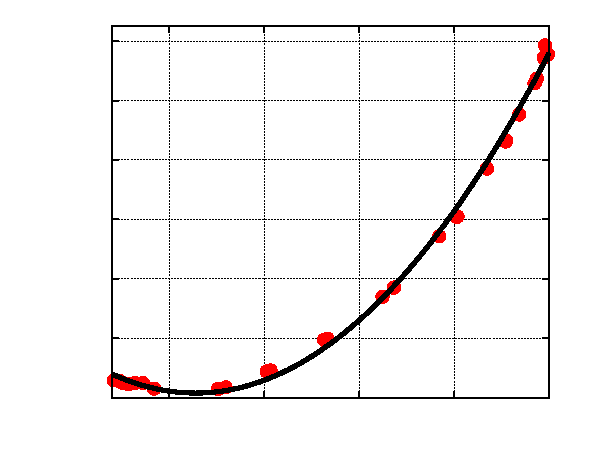
\includegraphics{CaelyxAverageDensity}}%
    \gplfronttext
  \end{picture}%
\endgroup

		\caption{Measured intensity at zero-angle of Caelyx as a function of the electron density of the aqueous iodixanol suspending medium. The function fitted to the experimental data is depicted in black: Average density is 346.39 nm$^{-3}$ and there is a offset of 1.56 cm$^{-1}$}
		\label{fig:CaelyxAverageDensity}
\end{figure}

From this calculation, a value of $\rho_0$ = (346.2 $\pm$ 1.2) nm$^{-3}$ is obtained which corresponds to the density of the liposomal nanocarrier and the precipitated drug combined. The uncertainty of 1.2 nm$^{-3}$ is associated with the vertical size of the focused X-ray beam. The obtained density is slightly higher than the value of 338 nm$^{-3}$ estimated for empty PEGylated liposomes \cite{kucerka_structure_2006} due to the presence of the doxorubicin-sulfate aggregate in the intraliposomal volume.

\section{Osmotic effects in liposomes}

The rigidity of the nanocarriers is a relevant property directly related with its drug delivery efficacy, the particle stability or the release rate of the encapsulated drug. In fact, some of these characteristics might change upon injection due to the osmotic pressure applied to the nanocarriers in the process. In the case of lipid vesicles, i.e. liposomes, the permeability of water through the phopholipid bilayer is a defining aspect of its physicochemical behavior. Although many aspects about the membrane permeability have been studied \cite{nagle_theory_2008, mathai_structural_2008, olbrich_water_2000}, the evaluation of the liposomes rigidity and its osmotic activity is still challenging.

The osmotic behavior of liposomes depends, basically, on their size and chemical composition. For example, the incorporation of cholesterol can vary the fluidity of the lipid bilayer. Larger liposomes tend to be osmotically active \cite{de_gier_osmotic_1993} and behave according to the Laplace law: the osmotic pressure needed to deform them decreases for increasing sizes. In the case of liposomal nanocarriers, the intraliposomal osmolality should be equal to the buffer outside of the liposomes to enhance the particle stability. 

\begin{figure}
	\centering
		% GNUPLOT: LaTeX picture with Postscript
\begingroup
  \makeatletter
  \providecommand\color[2][]{%
    \GenericError{(gnuplot) \space\space\space\@spaces}{%
      Package color not loaded in conjunction with
      terminal option `colourtext'%
    }{See the gnuplot documentation for explanation.%
    }{Either use 'blacktext' in gnuplot or load the package
      color.sty in LaTeX.}%
    \renewcommand\color[2][]{}%
  }%
  \providecommand\includegraphics[2][]{%
    \GenericError{(gnuplot) \space\space\space\@spaces}{%
      Package graphicx or graphics not loaded%
    }{See the gnuplot documentation for explanation.%
    }{The gnuplot epslatex terminal needs graphicx.sty or graphics.sty.}%
    \renewcommand\includegraphics[2][]{}%
  }%
  \providecommand\rotatebox[2]{#2}%
  \@ifundefined{ifGPcolor}{%
    \newif\ifGPcolor
    \GPcolortrue
  }{}%
  \@ifundefined{ifGPblacktext}{%
    \newif\ifGPblacktext
    \GPblacktextfalse
  }{}%
  % define a \g@addto@macro without @ in the name:
  \let\gplgaddtomacro\g@addto@macro
  % define empty templates for all commands taking text:
  \gdef\gplbacktext{}%
  \gdef\gplfronttext{}%
  \makeatother
  \ifGPblacktext
    % no textcolor at all
    \def\colorrgb#1{}%
    \def\colorgray#1{}%
  \else
    % gray or color?
    \ifGPcolor
      \def\colorrgb#1{\color[rgb]{#1}}%
      \def\colorgray#1{\color[gray]{#1}}%
      \expandafter\def\csname LTw\endcsname{\color{white}}%
      \expandafter\def\csname LTb\endcsname{\color{black}}%
      \expandafter\def\csname LTa\endcsname{\color{black}}%
      \expandafter\def\csname LT0\endcsname{\color[rgb]{1,0,0}}%
      \expandafter\def\csname LT1\endcsname{\color[rgb]{0,1,0}}%
      \expandafter\def\csname LT2\endcsname{\color[rgb]{0,0,1}}%
      \expandafter\def\csname LT3\endcsname{\color[rgb]{1,0,1}}%
      \expandafter\def\csname LT4\endcsname{\color[rgb]{0,1,1}}%
      \expandafter\def\csname LT5\endcsname{\color[rgb]{1,1,0}}%
      \expandafter\def\csname LT6\endcsname{\color[rgb]{0,0,0}}%
      \expandafter\def\csname LT7\endcsname{\color[rgb]{1,0.3,0}}%
      \expandafter\def\csname LT8\endcsname{\color[rgb]{0.5,0.5,0.5}}%
    \else
      % gray
      \def\colorrgb#1{\color{black}}%
      \def\colorgray#1{\color[gray]{#1}}%
      \expandafter\def\csname LTw\endcsname{\color{white}}%
      \expandafter\def\csname LTb\endcsname{\color{black}}%
      \expandafter\def\csname LTa\endcsname{\color{black}}%
      \expandafter\def\csname LT0\endcsname{\color{black}}%
      \expandafter\def\csname LT1\endcsname{\color{black}}%
      \expandafter\def\csname LT2\endcsname{\color{black}}%
      \expandafter\def\csname LT3\endcsname{\color{black}}%
      \expandafter\def\csname LT4\endcsname{\color{black}}%
      \expandafter\def\csname LT5\endcsname{\color{black}}%
      \expandafter\def\csname LT6\endcsname{\color{black}}%
      \expandafter\def\csname LT7\endcsname{\color{black}}%
      \expandafter\def\csname LT8\endcsname{\color{black}}%
    \fi
  \fi
  \setlength{\unitlength}{0.0500bp}%
  \begin{picture}(5668.00,4534.00)%
    \gplgaddtomacro\gplbacktext{%
      \csname LTb\endcsname%
      \put(814,1183){\makebox(0,0)[r]{\strut{} 340}}%
      \csname LTb\endcsname%
      \put(814,1885){\makebox(0,0)[r]{\strut{} 350}}%
      \csname LTb\endcsname%
      \put(814,2588){\makebox(0,0)[r]{\strut{} 360}}%
      \csname LTb\endcsname%
      \put(814,3291){\makebox(0,0)[r]{\strut{} 370}}%
      \csname LTb\endcsname%
      \put(814,3994){\makebox(0,0)[r]{\strut{} 380}}%
      \csname LTb\endcsname%
      \put(946,484){\makebox(0,0){\strut{} 0}}%
      \csname LTb\endcsname%
      \put(1377,484){\makebox(0,0){\strut{} 5}}%
      \csname LTb\endcsname%
      \put(1807,484){\makebox(0,0){\strut{} 10}}%
      \csname LTb\endcsname%
      \put(2238,484){\makebox(0,0){\strut{} 15}}%
      \csname LTb\endcsname%
      \put(2668,484){\makebox(0,0){\strut{} 20}}%
      \csname LTb\endcsname%
      \put(3099,484){\makebox(0,0){\strut{} 25}}%
      \csname LTb\endcsname%
      \put(3530,484){\makebox(0,0){\strut{} 30}}%
      \csname LTb\endcsname%
      \put(3960,484){\makebox(0,0){\strut{} 35}}%
      \csname LTb\endcsname%
      \put(4391,484){\makebox(0,0){\strut{} 40}}%
      \put(4523,704){\makebox(0,0)[l]{\strut{}0}}%
      \put(4523,1407){\makebox(0,0)[l]{\strut{}250}}%
      \put(4523,2006){\makebox(0,0)[l]{\strut{}500}}%
      \put(4523,2525){\makebox(0,0)[l]{\strut{}750}}%
      \put(4523,2977){\makebox(0,0)[l]{\strut{}1000}}%
      \put(4523,3375){\makebox(0,0)[l]{\strut{}1250}}%
      \put(4523,3728){\makebox(0,0)[l]{\strut{}1500}}%
      \put(4523,4043){\makebox(0,0)[l]{\strut{}1750}}%
      \put(176,2486){\rotatebox{-270}{\makebox(0,0){\strut{}Electron Density / nm$^{-3}$}}}%
      \put(5160,2486){\rotatebox{270}{\makebox(0,0){\strut{}Osmolality / mOsm kg$^{-1}$}}}%
      \put(2668,154){\makebox(0,0){\strut{}Sucrose Mass Fraction / $\%$}}%
    }%
    \gplgaddtomacro\gplfronttext{%
    }%
    \gplbacktext
    \put(0,0){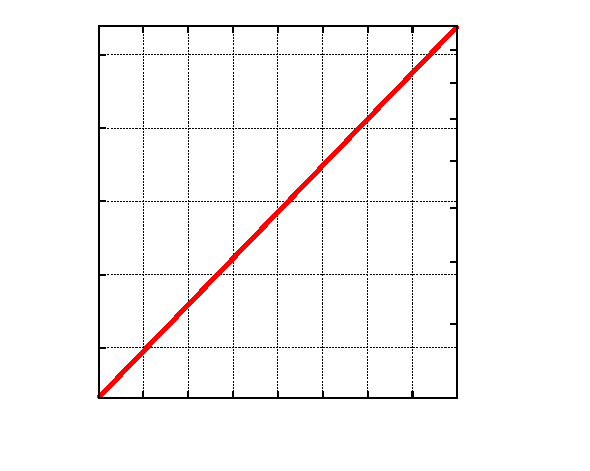
\includegraphics{OsmolalityElectronDensity}}%
    \gplfronttext
  \end{picture}%
\endgroup

		\caption{Relationship between solvent electron density and solvent osmolality for an aqueous sucrose solution.}
		\label{fig:OsmolalityElectronDensity}
\end{figure}

Therefore, it is an important question whether the incorporation of a drug into the intraliposomal volume might modify its osmotic activity. For example, the small size of Caelyx$\textregistered$ and the doxorubicin-sulfate aggregate in the intraliposomal volume create an extraordinary resistance against the buffer osmotic pressure in comparison to the empty liposomal particle. This effect can be studied by increasing systematically the osmolality of the suspending medium by increasing the sucrose concentration in the aqueous buffer. As shown in figure \ref{fig:OsmolalityElectronDensity}, the sucrose molecule acts simultenously as a contrast agent and as an instrument to increase the solvent osmolality. This enables the study of the osmotic effects in liposomes by the denstiy gradient technique with SAXS using aqueous sucrose as suspending medium, as it will be discussed in the following section.

Due to the constant osmolality of the suspending medium along the whole density gradient, no osmotic pressure effects were observed in the size or density of the liposomal drug Caelyx $\textregistered$ in the previous section \ref{sec:caelyx_size}. In this section, a thorough investigation of Caelyx $\textregistered$ under the effects of an increasing solvent osmolality is performed, complementary to the study of the empty liposomal nanocarrier under similar conditions. Besides, the consequences of PEGylation on the liposomal structure are also studied using this technique, focusing principally in its osmotic activity.
 
\subsection{Application to drug-stabilized liposomes}
\label{sec:OsmoticCaelyx}

By means of the density gradient technique, scattering curves of the liposomal doxorubicin were recorded at different sucrose concentrations of the suspending medium, i.e. at different buffer osmolalities, as shown in figure \ref{fig:CaelyxSucroseContinuousSAXS}. The X-ray scattering measurements were performed at two different detector-to-sample distances, as described in section \ref{sec:materials_caelyx}, in order to study a broader $q$-range, spanning from 0.03 to 5.55 nm$^{-1}$, and observe the 1,0-diffraction peak of the doxorubicin fiber-like precipitate around $q=2.3$ nm$^{-1}$ \cite{li_doxorubicin_1998}, as depicted in the figure \ref{fig:CaelyxSucroseContinuousWAXS} after proper background correction.

\begin{figure}
	\centering
		\subfloat[Osmotic effects in Caelyx by using sucrose as contrast agent]{\resizebox{0.44\linewidth}{!}{% GNUPLOT: LaTeX picture with Postscript
\begingroup
  \makeatletter
  \providecommand\color[2][]{%
    \GenericError{(gnuplot) \space\space\space\@spaces}{%
      Package color not loaded in conjunction with
      terminal option `colourtext'%
    }{See the gnuplot documentation for explanation.%
    }{Either use 'blacktext' in gnuplot or load the package
      color.sty in LaTeX.}%
    \renewcommand\color[2][]{}%
  }%
  \providecommand\includegraphics[2][]{%
    \GenericError{(gnuplot) \space\space\space\@spaces}{%
      Package graphicx or graphics not loaded%
    }{See the gnuplot documentation for explanation.%
    }{The gnuplot epslatex terminal needs graphicx.sty or graphics.sty.}%
    \renewcommand\includegraphics[2][]{}%
  }%
  \providecommand\rotatebox[2]{#2}%
  \@ifundefined{ifGPcolor}{%
    \newif\ifGPcolor
    \GPcolortrue
  }{}%
  \@ifundefined{ifGPblacktext}{%
    \newif\ifGPblacktext
    \GPblacktextfalse
  }{}%
  % define a \g@addto@macro without @ in the name:
  \let\gplgaddtomacro\g@addto@macro
  % define empty templates for all commands taking text:
  \gdef\gplbacktext{}%
  \gdef\gplfronttext{}%
  \makeatother
  \ifGPblacktext
    % no textcolor at all
    \def\colorrgb#1{}%
    \def\colorgray#1{}%
  \else
    % gray or color?
    \ifGPcolor
      \def\colorrgb#1{\color[rgb]{#1}}%
      \def\colorgray#1{\color[gray]{#1}}%
      \expandafter\def\csname LTw\endcsname{\color{white}}%
      \expandafter\def\csname LTb\endcsname{\color{black}}%
      \expandafter\def\csname LTa\endcsname{\color{black}}%
      \expandafter\def\csname LT0\endcsname{\color[rgb]{1,0,0}}%
      \expandafter\def\csname LT1\endcsname{\color[rgb]{0,1,0}}%
      \expandafter\def\csname LT2\endcsname{\color[rgb]{0,0,1}}%
      \expandafter\def\csname LT3\endcsname{\color[rgb]{1,0,1}}%
      \expandafter\def\csname LT4\endcsname{\color[rgb]{0,1,1}}%
      \expandafter\def\csname LT5\endcsname{\color[rgb]{1,1,0}}%
      \expandafter\def\csname LT6\endcsname{\color[rgb]{0,0,0}}%
      \expandafter\def\csname LT7\endcsname{\color[rgb]{1,0.3,0}}%
      \expandafter\def\csname LT8\endcsname{\color[rgb]{0.5,0.5,0.5}}%
    \else
      % gray
      \def\colorrgb#1{\color{black}}%
      \def\colorgray#1{\color[gray]{#1}}%
      \expandafter\def\csname LTw\endcsname{\color{white}}%
      \expandafter\def\csname LTb\endcsname{\color{black}}%
      \expandafter\def\csname LTa\endcsname{\color{black}}%
      \expandafter\def\csname LT0\endcsname{\color{black}}%
      \expandafter\def\csname LT1\endcsname{\color{black}}%
      \expandafter\def\csname LT2\endcsname{\color{black}}%
      \expandafter\def\csname LT3\endcsname{\color{black}}%
      \expandafter\def\csname LT4\endcsname{\color{black}}%
      \expandafter\def\csname LT5\endcsname{\color{black}}%
      \expandafter\def\csname LT6\endcsname{\color{black}}%
      \expandafter\def\csname LT7\endcsname{\color{black}}%
      \expandafter\def\csname LT8\endcsname{\color{black}}%
    \fi
  \fi
  \setlength{\unitlength}{0.0500bp}%
  \begin{picture}(5668.00,4534.00)%
    \gplgaddtomacro\gplbacktext{%
      \csname LTb\endcsname%
      \put(814,1053){\makebox(0,0)[r]{\strut{} 0.1}}%
      \csname LTb\endcsname%
      \put(814,2210){\makebox(0,0)[r]{\strut{} 1}}%
      \csname LTb\endcsname%
      \put(814,3368){\makebox(0,0)[r]{\strut{} 10}}%
      \csname LTb\endcsname%
      \put(1434,484){\makebox(0,0){\strut{} 0.05}}%
      \csname LTb\endcsname%
      \put(2096,484){\makebox(0,0){\strut{} 0.1}}%
      \csname LTb\endcsname%
      \put(2758,484){\makebox(0,0){\strut{} 0.2}}%
      \csname LTb\endcsname%
      \put(3633,484){\makebox(0,0){\strut{} 0.5}}%
      \csname LTb\endcsname%
      \put(4295,484){\makebox(0,0){\strut{} 1}}%
      \put(176,2266){\rotatebox{-270}{\makebox(0,0){\strut{}Scattering Intensity / cm$^{-1}$}}}%
      \put(2687,154){\makebox(0,0){\strut{}$q$ / nm$^{-1}$}}%
    }%
    \gplgaddtomacro\gplfronttext{%
      \csname LTb\endcsname%
      \put(4822,778){\makebox(0,0)[l]{\strut{}\smaller 200}}%
      \put(4822,1149){\makebox(0,0)[l]{\strut{}\smaller 400}}%
      \put(4822,1520){\makebox(0,0)[l]{\strut{}\smaller 600}}%
      \put(4822,1892){\makebox(0,0)[l]{\strut{}\smaller 800}}%
      \put(4822,2263){\makebox(0,0)[l]{\strut{}\smaller 1000}}%
      \put(4822,2635){\makebox(0,0)[l]{\strut{}\smaller 1200}}%
      \put(4822,3006){\makebox(0,0)[l]{\strut{}\smaller 1400}}%
      \put(4822,3377){\makebox(0,0)[l]{\strut{}\smaller 1600}}%
      \put(4822,3749){\makebox(0,0)[l]{\strut{}\smaller 1800}}%
      \put(4822,4120){\makebox(0,0)[l]{\strut{}\smaller 2000}}%
      \put(5483,2486){\rotatebox{-90}{\makebox(0,0){\strut{}\smaller Solvent Osmolality / mOsm kg$^{-1}$}}}%
    }%
    \gplbacktext
    \put(0,0){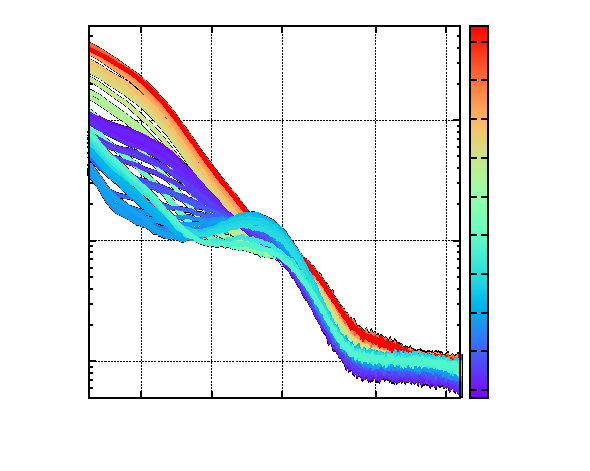
\includegraphics{CaelyxSucroseContinuousSAXS}}%
    \gplfronttext
  \end{picture}%
\endgroup
}\label{fig:CaelyxSucroseContinuousSAXS}}
		\subfloat[Isoscattering point intensity at 2 different setups: Osmotic threshold at 740 mOsm kg$^{-1}$]{\resizebox{0.44\linewidth}{!}{% GNUPLOT: LaTeX picture with Postscript
\begingroup
  \makeatletter
  \providecommand\color[2][]{%
    \GenericError{(gnuplot) \space\space\space\@spaces}{%
      Package color not loaded in conjunction with
      terminal option `colourtext'%
    }{See the gnuplot documentation for explanation.%
    }{Either use 'blacktext' in gnuplot or load the package
      color.sty in LaTeX.}%
    \renewcommand\color[2][]{}%
  }%
  \providecommand\includegraphics[2][]{%
    \GenericError{(gnuplot) \space\space\space\@spaces}{%
      Package graphicx or graphics not loaded%
    }{See the gnuplot documentation for explanation.%
    }{The gnuplot epslatex terminal needs graphicx.sty or graphics.sty.}%
    \renewcommand\includegraphics[2][]{}%
  }%
  \providecommand\rotatebox[2]{#2}%
  \@ifundefined{ifGPcolor}{%
    \newif\ifGPcolor
    \GPcolortrue
  }{}%
  \@ifundefined{ifGPblacktext}{%
    \newif\ifGPblacktext
    \GPblacktextfalse
  }{}%
  % define a \g@addto@macro without @ in the name:
  \let\gplgaddtomacro\g@addto@macro
  % define empty templates for all commands taking text:
  \gdef\gplbacktext{}%
  \gdef\gplfronttext{}%
  \makeatother
  \ifGPblacktext
    % no textcolor at all
    \def\colorrgb#1{}%
    \def\colorgray#1{}%
  \else
    % gray or color?
    \ifGPcolor
      \def\colorrgb#1{\color[rgb]{#1}}%
      \def\colorgray#1{\color[gray]{#1}}%
      \expandafter\def\csname LTw\endcsname{\color{white}}%
      \expandafter\def\csname LTb\endcsname{\color{black}}%
      \expandafter\def\csname LTa\endcsname{\color{black}}%
      \expandafter\def\csname LT0\endcsname{\color[rgb]{1,0,0}}%
      \expandafter\def\csname LT1\endcsname{\color[rgb]{0,1,0}}%
      \expandafter\def\csname LT2\endcsname{\color[rgb]{0,0,1}}%
      \expandafter\def\csname LT3\endcsname{\color[rgb]{1,0,1}}%
      \expandafter\def\csname LT4\endcsname{\color[rgb]{0,1,1}}%
      \expandafter\def\csname LT5\endcsname{\color[rgb]{1,1,0}}%
      \expandafter\def\csname LT6\endcsname{\color[rgb]{0,0,0}}%
      \expandafter\def\csname LT7\endcsname{\color[rgb]{1,0.3,0}}%
      \expandafter\def\csname LT8\endcsname{\color[rgb]{0.5,0.5,0.5}}%
    \else
      % gray
      \def\colorrgb#1{\color{black}}%
      \def\colorgray#1{\color[gray]{#1}}%
      \expandafter\def\csname LTw\endcsname{\color{white}}%
      \expandafter\def\csname LTb\endcsname{\color{black}}%
      \expandafter\def\csname LTa\endcsname{\color{black}}%
      \expandafter\def\csname LT0\endcsname{\color{black}}%
      \expandafter\def\csname LT1\endcsname{\color{black}}%
      \expandafter\def\csname LT2\endcsname{\color{black}}%
      \expandafter\def\csname LT3\endcsname{\color{black}}%
      \expandafter\def\csname LT4\endcsname{\color{black}}%
      \expandafter\def\csname LT5\endcsname{\color{black}}%
      \expandafter\def\csname LT6\endcsname{\color{black}}%
      \expandafter\def\csname LT7\endcsname{\color{black}}%
      \expandafter\def\csname LT8\endcsname{\color{black}}%
    \fi
  \fi
  \setlength{\unitlength}{0.0500bp}%
  \begin{picture}(5668.00,4534.00)%
    \gplgaddtomacro\gplbacktext{%
      \csname LTb\endcsname%
      \put(176,2486){\rotatebox{-270}{\makebox(0,0){\strut{}Intensity at $q=0.123$ nm$^{-1}$ / cm$^{-1}$}}}%
      \put(3108,154){\makebox(0,0){\strut{}Solvent Osmolality / mOsm kg$^{-1}$}}%
    }%
    \gplgaddtomacro\gplfronttext{%
      \csname LTb\endcsname%
      \put(4788,1331){\makebox(0,0)[r]{\strut{}\smaller SAXS}}%
      \csname LTb\endcsname%
      \put(4788,1001){\makebox(0,0)[r]{\strut{}\smaller WAXS}}%
      \csname LTb\endcsname%
      \put(814,704){\makebox(0,0)[r]{\strut{} 0.8}}%
      \csname LTb\endcsname%
      \put(814,1100){\makebox(0,0)[r]{\strut{} 1}}%
      \csname LTb\endcsname%
      \put(814,1496){\makebox(0,0)[r]{\strut{} 1.2}}%
      \csname LTb\endcsname%
      \put(814,1892){\makebox(0,0)[r]{\strut{} 1.4}}%
      \csname LTb\endcsname%
      \put(814,2288){\makebox(0,0)[r]{\strut{} 1.6}}%
      \csname LTb\endcsname%
      \put(814,2685){\makebox(0,0)[r]{\strut{} 1.8}}%
      \csname LTb\endcsname%
      \put(814,3081){\makebox(0,0)[r]{\strut{} 2}}%
      \csname LTb\endcsname%
      \put(814,3477){\makebox(0,0)[r]{\strut{} 2.2}}%
      \csname LTb\endcsname%
      \put(814,3873){\makebox(0,0)[r]{\strut{} 2.4}}%
      \csname LTb\endcsname%
      \put(814,4269){\makebox(0,0)[r]{\strut{} 2.6}}%
      \csname LTb\endcsname%
      \put(1270,484){\makebox(0,0){\strut{} 300}}%
      \csname LTb\endcsname%
      \put(1919,484){\makebox(0,0){\strut{} 600}}%
      \csname LTb\endcsname%
      \put(2568,484){\makebox(0,0){\strut{} 900}}%
      \csname LTb\endcsname%
      \put(3217,484){\makebox(0,0){\strut{} 1200}}%
      \csname LTb\endcsname%
      \put(3865,484){\makebox(0,0){\strut{} 1500}}%
      \csname LTb\endcsname%
      \put(4514,484){\makebox(0,0){\strut{} 1800}}%
      \csname LTb\endcsname%
      \put(5163,484){\makebox(0,0){\strut{} 2100}}%
      \put(2287,3477){\makebox(0,0)[l]{\strut{}\smaller \shortstack{Osmotic\\shrinkage}}}%
      \put(1465,3477){\makebox(0,0){\strut{}\smaller \shortstack{Constant\\shape\\and size}}}%
    }%
    \gplbacktext
    \put(0,0){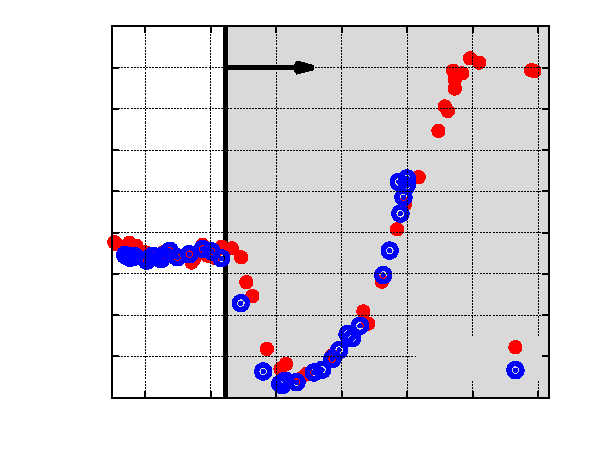
\includegraphics{CaelyxSucroseContinuousSAXSIsopoint}}%
    \gplfronttext
  \end{picture}%
\endgroup
}\label{fig:CaelyxSucroseContinuousSAXSIsopoint}}
		\caption{Scattering curves of Caelyx in an aqueous sucrose density gradient calibrated to the osmolality of the suspending medium. Intensity of the first isoscattering point depending on the aqueous sucrose solution osmolality is shown with black dots.}
\end{figure}

As discussed in the previous section, by increasing the electron density of the suspending medium, the scattering curves of the drug carrier change drastically due to contrast variation. In the case of the aqueous sucrose gradient shown in figure \ref{fig:CaelyxSucroseContinuousSAXS}, this effect is also observed and strongly resembles the curves measured with the Optiprep $\textregistered$ density gradient depicted in figure \ref{fig:CaelyxIodixanolContinuousSAXS}. Nevertheless, upon a certain sucrose concentration (greenish and reddish colored curves in figure \ref{fig:CaelyxSucroseContinuousSAXS}), the features of the scattering curves disappear abruptly, because the suspending medium osmolality is so high that it induces morphological changes in the liposomal structure and, consequently, the scattering form factor of the particles changes.

This effect can be quantified by examining the intensity of the first isoscattering point at $q^{\star}_1 = 0.123$ nm$^{-1}$, because the scattered intensity at this point should be independent of the electron density of the solvent, as observed with the Optiprep $\textregistered$ gradient. The isoscattering point intensity as a function of the suspending medium osmolality is shown in figure \ref{fig:CaelyxSucroseContinuousSAXSIsopoint} and there is a clear osmolality threshold at 670 mOsm kg$^{-1}$. Above this threshold, the osmotic pressure at the liposomal bilayer is so high that the liposome starts shrinking and changes its size, structure and, consequently, scattering form factor. The increased resistance against osmotic pressure, more than double the blood plasma osmolality and much higher than the osmolality needed to shrink empty PEGylated liposomes \cite{varga_osmotic_2014}, is explained by the encapsulation of doxorubicin inside the liposome.

The large osmotic pressure produces a reversible shrinkage of the liposome though it is not capable of cracking it. This was proved in an additional experiment by increasing the osmolality of the buffer to 1333.6 mOsm kg$^{-1}$ with a sucrose mass fraction of 31.4$\%$ and then reducing it to 565.4 mOsm kg-1 by adding distilled water. The solvent with high osmolality produced a featureless scattering curve, as expected from figure \ref{fig:CaelyxSucroseContinuousSAXS}, whereas, after reducing the osmotic pressure, the scattering curve was the same as the measured Caelyx$\textregistered$ curve with the corresponding electron density, which gives evidence that the osmotic shrinkage process is reversible.

\begin{figure}
	\centering
		\subfloat[Osmotic effects in Caelys by using sucrose as contrast agent]{\resizebox{0.44\linewidth}{!}{% GNUPLOT: LaTeX picture with Postscript
\begingroup
  \makeatletter
  \providecommand\color[2][]{%
    \GenericError{(gnuplot) \space\space\space\@spaces}{%
      Package color not loaded in conjunction with
      terminal option `colourtext'%
    }{See the gnuplot documentation for explanation.%
    }{Either use 'blacktext' in gnuplot or load the package
      color.sty in LaTeX.}%
    \renewcommand\color[2][]{}%
  }%
  \providecommand\includegraphics[2][]{%
    \GenericError{(gnuplot) \space\space\space\@spaces}{%
      Package graphicx or graphics not loaded%
    }{See the gnuplot documentation for explanation.%
    }{The gnuplot epslatex terminal needs graphicx.sty or graphics.sty.}%
    \renewcommand\includegraphics[2][]{}%
  }%
  \providecommand\rotatebox[2]{#2}%
  \@ifundefined{ifGPcolor}{%
    \newif\ifGPcolor
    \GPcolortrue
  }{}%
  \@ifundefined{ifGPblacktext}{%
    \newif\ifGPblacktext
    \GPblacktextfalse
  }{}%
  % define a \g@addto@macro without @ in the name:
  \let\gplgaddtomacro\g@addto@macro
  % define empty templates for all commands taking text:
  \gdef\gplbacktext{}%
  \gdef\gplfronttext{}%
  \makeatother
  \ifGPblacktext
    % no textcolor at all
    \def\colorrgb#1{}%
    \def\colorgray#1{}%
  \else
    % gray or color?
    \ifGPcolor
      \def\colorrgb#1{\color[rgb]{#1}}%
      \def\colorgray#1{\color[gray]{#1}}%
      \expandafter\def\csname LTw\endcsname{\color{white}}%
      \expandafter\def\csname LTb\endcsname{\color{black}}%
      \expandafter\def\csname LTa\endcsname{\color{black}}%
      \expandafter\def\csname LT0\endcsname{\color[rgb]{1,0,0}}%
      \expandafter\def\csname LT1\endcsname{\color[rgb]{0,1,0}}%
      \expandafter\def\csname LT2\endcsname{\color[rgb]{0,0,1}}%
      \expandafter\def\csname LT3\endcsname{\color[rgb]{1,0,1}}%
      \expandafter\def\csname LT4\endcsname{\color[rgb]{0,1,1}}%
      \expandafter\def\csname LT5\endcsname{\color[rgb]{1,1,0}}%
      \expandafter\def\csname LT6\endcsname{\color[rgb]{0,0,0}}%
      \expandafter\def\csname LT7\endcsname{\color[rgb]{1,0.3,0}}%
      \expandafter\def\csname LT8\endcsname{\color[rgb]{0.5,0.5,0.5}}%
    \else
      % gray
      \def\colorrgb#1{\color{black}}%
      \def\colorgray#1{\color[gray]{#1}}%
      \expandafter\def\csname LTw\endcsname{\color{white}}%
      \expandafter\def\csname LTb\endcsname{\color{black}}%
      \expandafter\def\csname LTa\endcsname{\color{black}}%
      \expandafter\def\csname LT0\endcsname{\color{black}}%
      \expandafter\def\csname LT1\endcsname{\color{black}}%
      \expandafter\def\csname LT2\endcsname{\color{black}}%
      \expandafter\def\csname LT3\endcsname{\color{black}}%
      \expandafter\def\csname LT4\endcsname{\color{black}}%
      \expandafter\def\csname LT5\endcsname{\color{black}}%
      \expandafter\def\csname LT6\endcsname{\color{black}}%
      \expandafter\def\csname LT7\endcsname{\color{black}}%
      \expandafter\def\csname LT8\endcsname{\color{black}}%
    \fi
  \fi
  \setlength{\unitlength}{0.0500bp}%
  \begin{picture}(5668.00,4534.00)%
    \gplgaddtomacro\gplbacktext{%
      \csname LTb\endcsname%
      \put(1122,704){\makebox(0,0)[r]{\strut{} 0}}%
      \csname LTb\endcsname%
      \put(1122,1417){\makebox(0,0)[r]{\strut{} 0.0002}}%
      \csname LTb\endcsname%
      \put(1122,2130){\makebox(0,0)[r]{\strut{} 0.0004}}%
      \csname LTb\endcsname%
      \put(1122,2843){\makebox(0,0)[r]{\strut{} 0.0006}}%
      \csname LTb\endcsname%
      \put(1122,3556){\makebox(0,0)[r]{\strut{} 0.0008}}%
      \csname LTb\endcsname%
      \put(1122,4269){\makebox(0,0)[r]{\strut{} 0.001}}%
      \put(220,2266){\rotatebox{-270}{\makebox(0,0){\strut{}Scattering Intensity / cm$^{-1}$}}}%
      \put(2857,154){\makebox(0,0){\strut{}$q$ / nm$^{-1}$}}%
    }%
    \gplgaddtomacro\gplfronttext{%
      \csname LTb\endcsname%
      \put(4701,704){\makebox(0,0)[l]{\strut{}\fsmedium 200}}%
      \put(4701,1252){\makebox(0,0)[l]{\strut{}\fsmedium 400}}%
      \put(4701,1800){\makebox(0,0)[l]{\strut{}\fsmedium 600}}%
      \put(4701,2349){\makebox(0,0)[l]{\strut{}\fsmedium 800}}%
      \put(4701,2897){\makebox(0,0)[l]{\strut{}\fsmedium 1000}}%
      \put(4701,3446){\makebox(0,0)[l]{\strut{}\fsmedium 1200}}%
      \put(4701,3994){\makebox(0,0)[l]{\strut{}\fsmedium 1400}}%
      \put(5559,2486){\rotatebox{-90}{\makebox(0,0){\strut{}\fsmedium Solvent Osmolality / mOsm kg$^{-1}$}}}%
    }%
    \gplbacktext
    \put(0,0){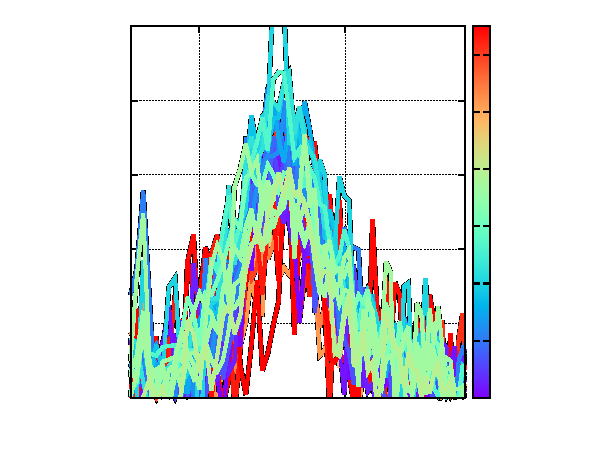
\includegraphics{CaelyxSucroseContinuousWAXS}}%
    \gplfronttext
  \end{picture}%
\endgroup
}\label{fig:CaelyxSucroseContinuousWAXS}}
		\subfloat[Diffraction peak width and position]{\resizebox{0.44\linewidth}{!}{% GNUPLOT: LaTeX picture with Postscript
\begingroup
  \makeatletter
  \providecommand\color[2][]{%
    \GenericError{(gnuplot) \space\space\space\@spaces}{%
      Package color not loaded in conjunction with
      terminal option `colourtext'%
    }{See the gnuplot documentation for explanation.%
    }{Either use 'blacktext' in gnuplot or load the package
      color.sty in LaTeX.}%
    \renewcommand\color[2][]{}%
  }%
  \providecommand\includegraphics[2][]{%
    \GenericError{(gnuplot) \space\space\space\@spaces}{%
      Package graphicx or graphics not loaded%
    }{See the gnuplot documentation for explanation.%
    }{The gnuplot epslatex terminal needs graphicx.sty or graphics.sty.}%
    \renewcommand\includegraphics[2][]{}%
  }%
  \providecommand\rotatebox[2]{#2}%
  \@ifundefined{ifGPcolor}{%
    \newif\ifGPcolor
    \GPcolortrue
  }{}%
  \@ifundefined{ifGPblacktext}{%
    \newif\ifGPblacktext
    \GPblacktextfalse
  }{}%
  % define a \g@addto@macro without @ in the name:
  \let\gplgaddtomacro\g@addto@macro
  % define empty templates for all commands taking text:
  \gdef\gplbacktext{}%
  \gdef\gplfronttext{}%
  \makeatother
  \ifGPblacktext
    % no textcolor at all
    \def\colorrgb#1{}%
    \def\colorgray#1{}%
  \else
    % gray or color?
    \ifGPcolor
      \def\colorrgb#1{\color[rgb]{#1}}%
      \def\colorgray#1{\color[gray]{#1}}%
      \expandafter\def\csname LTw\endcsname{\color{white}}%
      \expandafter\def\csname LTb\endcsname{\color{black}}%
      \expandafter\def\csname LTa\endcsname{\color{black}}%
      \expandafter\def\csname LT0\endcsname{\color[rgb]{1,0,0}}%
      \expandafter\def\csname LT1\endcsname{\color[rgb]{0,1,0}}%
      \expandafter\def\csname LT2\endcsname{\color[rgb]{0,0,1}}%
      \expandafter\def\csname LT3\endcsname{\color[rgb]{1,0,1}}%
      \expandafter\def\csname LT4\endcsname{\color[rgb]{0,1,1}}%
      \expandafter\def\csname LT5\endcsname{\color[rgb]{1,1,0}}%
      \expandafter\def\csname LT6\endcsname{\color[rgb]{0,0,0}}%
      \expandafter\def\csname LT7\endcsname{\color[rgb]{1,0.3,0}}%
      \expandafter\def\csname LT8\endcsname{\color[rgb]{0.5,0.5,0.5}}%
    \else
      % gray
      \def\colorrgb#1{\color{black}}%
      \def\colorgray#1{\color[gray]{#1}}%
      \expandafter\def\csname LTw\endcsname{\color{white}}%
      \expandafter\def\csname LTb\endcsname{\color{black}}%
      \expandafter\def\csname LTa\endcsname{\color{black}}%
      \expandafter\def\csname LT0\endcsname{\color{black}}%
      \expandafter\def\csname LT1\endcsname{\color{black}}%
      \expandafter\def\csname LT2\endcsname{\color{black}}%
      \expandafter\def\csname LT3\endcsname{\color{black}}%
      \expandafter\def\csname LT4\endcsname{\color{black}}%
      \expandafter\def\csname LT5\endcsname{\color{black}}%
      \expandafter\def\csname LT6\endcsname{\color{black}}%
      \expandafter\def\csname LT7\endcsname{\color{black}}%
      \expandafter\def\csname LT8\endcsname{\color{black}}%
    \fi
  \fi
  \setlength{\unitlength}{0.0500bp}%
  \begin{picture}(5668.00,4534.00)%
    \gplgaddtomacro\gplbacktext{%
      \csname LTb\endcsname%
      \put(814,1028){\makebox(0,0)[r]{\strut{}-1}}%
      \csname LTb\endcsname%
      \put(814,1838){\makebox(0,0)[r]{\strut{}-0.5}}%
      \csname LTb\endcsname%
      \put(814,2649){\makebox(0,0)[r]{\strut{} 0}}%
      \csname LTb\endcsname%
      \put(814,3459){\makebox(0,0)[r]{\strut{} 0.5}}%
      \csname LTb\endcsname%
      \put(814,4269){\makebox(0,0)[r]{\strut{} 1}}%
      \csname LTb\endcsname%
      \put(1084,484){\makebox(0,0){\strut{} 250}}%
      \csname LTb\endcsname%
      \put(1922,484){\makebox(0,0){\strut{} 500}}%
      \csname LTb\endcsname%
      \put(2759,484){\makebox(0,0){\strut{} 750}}%
      \csname LTb\endcsname%
      \put(3596,484){\makebox(0,0){\strut{} 1000}}%
      \csname LTb\endcsname%
      \put(4434,484){\makebox(0,0){\strut{} 1250}}%
      \csname LTb\endcsname%
      \put(5271,484){\makebox(0,0){\strut{} 1500}}%
      \put(176,2486){\rotatebox{-270}{\makebox(0,0){\strut{}Diffraction Peak Deviation / $\%$}}}%
      \put(3108,154){\makebox(0,0){\strut{}Solvent Osmolality / mOsm kg$^{-1}$}}%
    }%
    \gplgaddtomacro\gplfronttext{%
    }%
    \gplbacktext
    \put(0,0){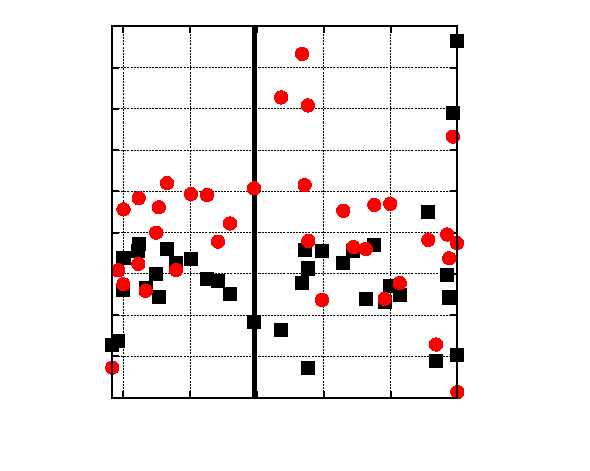
\includegraphics{CaelyxSucroseContinuousWAXSDiffraction}}%
    \gplfronttext
  \end{picture}%
\endgroup
}\label{fig:CaelyxSucroseContinuousWAXSDiffraction}}
		\caption{Measured in WAXS, the $q$-region where the doxorubicin diffraction peak appears can be observed. With black symbols, the shift of the doxorubicin-aggregate diffraction peak from $q=0.123$ nm$^{-1}$ is displayed The mean width (FWHM) is 0.333  nm$^{-1}$}
\end{figure}

The behavior of the nano-drug for an increasing solvent osmolality can be further studied by evaluating the crystal structure of the doxorubicin aggregate, represented by the diffraction peak observed in the figure \ref{fig:CaelyxSucroseContinuousWAXS}. The position of the peak in the reciprocal space depending on the suspending medium osmolality is depicted in figure \ref{fig:CaelyxSucroseContinuousWAXSDiffraction} and shows that its position deviates less than 1 $\%$ from the weighted average $q=2.28$ nm$^{-1}$ along the whole osmolality range. This proves that the fiber-like structure of the drug inside the liposome is also constant during the osmotic shrinkage of the liposomes. The measured position of the (1,0) diffraction peak matches exactly the value measured from doxorubicin-sulfate complexes in solution \cite{lasic_gelation_1992}.\textcolor{blue}{It can also be observed in figure \ref{fig:CaelyxSucroseContinuousWAXSDiffraction} how the width of the diffraction peak does not change sifnificantly along the osmolality range and thus, according to the Debye-Scherrer equation, the size of the precipated doxorubicin remains stable upon the osmotic shrinkage.}

\begin{figure}
	\centering
		% GNUPLOT: LaTeX picture with Postscript
\begingroup
  \makeatletter
  \providecommand\color[2][]{%
    \GenericError{(gnuplot) \space\space\space\@spaces}{%
      Package color not loaded in conjunction with
      terminal option `colourtext'%
    }{See the gnuplot documentation for explanation.%
    }{Either use 'blacktext' in gnuplot or load the package
      color.sty in LaTeX.}%
    \renewcommand\color[2][]{}%
  }%
  \providecommand\includegraphics[2][]{%
    \GenericError{(gnuplot) \space\space\space\@spaces}{%
      Package graphicx or graphics not loaded%
    }{See the gnuplot documentation for explanation.%
    }{The gnuplot epslatex terminal needs graphicx.sty or graphics.sty.}%
    \renewcommand\includegraphics[2][]{}%
  }%
  \providecommand\rotatebox[2]{#2}%
  \@ifundefined{ifGPcolor}{%
    \newif\ifGPcolor
    \GPcolortrue
  }{}%
  \@ifundefined{ifGPblacktext}{%
    \newif\ifGPblacktext
    \GPblacktextfalse
  }{}%
  % define a \g@addto@macro without @ in the name:
  \let\gplgaddtomacro\g@addto@macro
  % define empty templates for all commands taking text:
  \gdef\gplbacktext{}%
  \gdef\gplfronttext{}%
  \makeatother
  \ifGPblacktext
    % no textcolor at all
    \def\colorrgb#1{}%
    \def\colorgray#1{}%
  \else
    % gray or color?
    \ifGPcolor
      \def\colorrgb#1{\color[rgb]{#1}}%
      \def\colorgray#1{\color[gray]{#1}}%
      \expandafter\def\csname LTw\endcsname{\color{white}}%
      \expandafter\def\csname LTb\endcsname{\color{black}}%
      \expandafter\def\csname LTa\endcsname{\color{black}}%
      \expandafter\def\csname LT0\endcsname{\color[rgb]{1,0,0}}%
      \expandafter\def\csname LT1\endcsname{\color[rgb]{0,1,0}}%
      \expandafter\def\csname LT2\endcsname{\color[rgb]{0,0,1}}%
      \expandafter\def\csname LT3\endcsname{\color[rgb]{1,0,1}}%
      \expandafter\def\csname LT4\endcsname{\color[rgb]{0,1,1}}%
      \expandafter\def\csname LT5\endcsname{\color[rgb]{1,1,0}}%
      \expandafter\def\csname LT6\endcsname{\color[rgb]{0,0,0}}%
      \expandafter\def\csname LT7\endcsname{\color[rgb]{1,0.3,0}}%
      \expandafter\def\csname LT8\endcsname{\color[rgb]{0.5,0.5,0.5}}%
    \else
      % gray
      \def\colorrgb#1{\color{black}}%
      \def\colorgray#1{\color[gray]{#1}}%
      \expandafter\def\csname LTw\endcsname{\color{white}}%
      \expandafter\def\csname LTb\endcsname{\color{black}}%
      \expandafter\def\csname LTa\endcsname{\color{black}}%
      \expandafter\def\csname LT0\endcsname{\color{black}}%
      \expandafter\def\csname LT1\endcsname{\color{black}}%
      \expandafter\def\csname LT2\endcsname{\color{black}}%
      \expandafter\def\csname LT3\endcsname{\color{black}}%
      \expandafter\def\csname LT4\endcsname{\color{black}}%
      \expandafter\def\csname LT5\endcsname{\color{black}}%
      \expandafter\def\csname LT6\endcsname{\color{black}}%
      \expandafter\def\csname LT7\endcsname{\color{black}}%
      \expandafter\def\csname LT8\endcsname{\color{black}}%
    \fi
  \fi
  \setlength{\unitlength}{0.0500bp}%
  \begin{picture}(5668.00,4534.00)%
    \gplgaddtomacro\gplbacktext{%
      \csname LTb\endcsname%
      \put(946,638){\makebox(0,0)[r]{\strut{} 0}}%
      \csname LTb\endcsname%
      \put(946,1243){\makebox(0,0)[r]{\strut{} 0.05}}%
      \csname LTb\endcsname%
      \put(946,1848){\makebox(0,0)[r]{\strut{} 0.1}}%
      \csname LTb\endcsname%
      \put(946,2454){\makebox(0,0)[r]{\strut{} 0.15}}%
      \csname LTb\endcsname%
      \put(946,3059){\makebox(0,0)[r]{\strut{} 0.2}}%
      \csname LTb\endcsname%
      \put(946,3664){\makebox(0,0)[r]{\strut{} 0.25}}%
      \csname LTb\endcsname%
      \put(946,4269){\makebox(0,0)[r]{\strut{} 0.3}}%
      \csname LTb\endcsname%
      \put(1194,418){\makebox(0,0){\strut{} 0.1}}%
      \csname LTb\endcsname%
      \put(2359,418){\makebox(0,0){\strut{} 0.15}}%
      \csname LTb\endcsname%
      \put(3524,418){\makebox(0,0){\strut{} 0.2}}%
      \csname LTb\endcsname%
      \put(4689,418){\makebox(0,0){\strut{} 0.25}}%
      \put(176,2453){\rotatebox{-270}{\makebox(0,0){\strut{}Relative Standard Deviation}}}%
      \put(3174,154){\makebox(0,0){\strut{}$q$ / nm$^{-1}$}}%
    }%
    \gplgaddtomacro\gplfronttext{%
      \csname LTb\endcsname%
      \put(4548,4041){\makebox(0,0)[r]{\strut{}\smaller Optiprep}}%
      \csname LTb\endcsname%
      \put(4548,3711){\makebox(0,0)[r]{\strut{}\smaller Aqueous sucrose}}%
    }%
    \gplbacktext
    \put(0,0){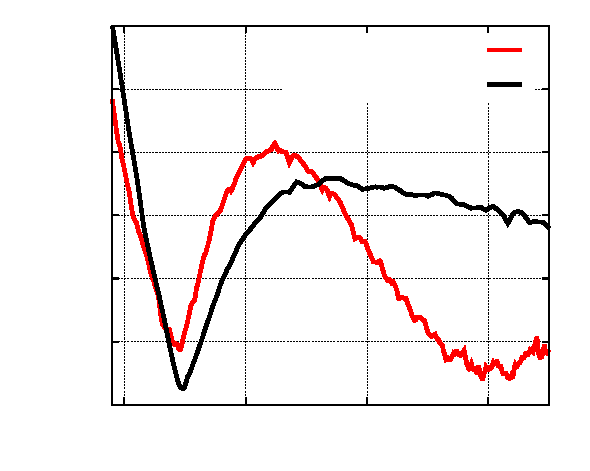
\includegraphics{CaelyxIsopointComparison}}%
    \gplfronttext
  \end{picture}%
\endgroup

		\caption{Isoscattering point position quantified by the calculation of the relative standard deviation of the scattering curves for different solvent density gradients. In the case of the aqueous sucrose solution (black line), only the scattering curves below the osmolality threshold were employed for the calculation.}
		\label{fig:CaelyxIsopointComparison}
\end{figure}

To conclude this section, the diameter obtained from the isoscattering position in the aqueous iodixanol solution can be compared with what is measured in an aqueous sucrose suspending medium. In the latter, if only the scattering curves below this osmolality threshold are considered, the relative standard deviation for each $q$ value reveals a pronounced minimum for the first isoscattering point as depicted in figure \ref{fig:CaelyxIsopointComparison}. When comparing this result with the relative standard deviation curve obtained from the Optiprep $\textregistered$ contrast variation measurements, both values for the size of the drug carrier agree remarkably well within 0.8 $\%$. This reflects the independence of the technique from the contrast agent added to the suspending medium and shows the repeatability of the results.


\subsection{Does PEGylation affect the osmotic activity of liposomes?}

Typically, unilamellar liposomes present a very narrow size distribution and spherical shape, whose diameter ranges from 50 nm to some hundreds of nanometers, and emerge as suitable nanocarriers for drug delivery. The covalent attachment of biocompatible polymers can improve the liposome stability. For example, polyetyhlene glycol (PEG) shows very low toxicity \cite{yamaoka_distribution_1994} and is a widely used stabilizer \cite{sou_polyethylene_2000}. PEGylated liposomal formulations, also called sterically stabilized liposomes (SSL), show longer blood circulation times \emph{in vivo} \cite{barenholz_liposome_2001} and exhibit a slow drug release rate. PEG-modified liposomes have become of importance lately due to their increased drug pharmakinetics, decreased plasma clearance and improved patient convenience \cite{gabizon_polyethylene_1997,harris_effect_2003}. Therefore, the self-assembly of lipid structures in the presence of PEG moieties has been studied for different lipids \cite{lee_coarse-grained_2011}.

The incorporation of biocompatible polymers increases the phospholipid bilayer strength and enhances the vesicle rigidity, which relates to the increase of the bending modulus \cite{liang_effect_2005, sou_polyethylene_2000}. The higher membrane stiffness of SSLs has been extensively characterized with methods such as Atomic Force Microscopy (AFM) \cite{spyratou_atomic_2009} though other techniques such as light scattering have found a higher osmotic activity in SSLs in comparison to their non-PEGylated counterparts when incubated in serum \cite{wolfram_shrinkage_2014}. Further investigations about the relationship between PEGylation and the liposomal osmotic behavior in suspension are essential. In the following work, the different response of SSLs and plain liposomes to osmotic pressure is studied with SAXS. The creation of multilamellar domains in the phospholipid layer is evaluated and the role of the PEG moieties in the membrane resilience is also analyzed.

\begin{figure}
	\centering
		% GNUPLOT: LaTeX picture with Postscript
\begingroup
  \makeatletter
  \providecommand\color[2][]{%
    \GenericError{(gnuplot) \space\space\space\@spaces}{%
      Package color not loaded in conjunction with
      terminal option `colourtext'%
    }{See the gnuplot documentation for explanation.%
    }{Either use 'blacktext' in gnuplot or load the package
      color.sty in LaTeX.}%
    \renewcommand\color[2][]{}%
  }%
  \providecommand\includegraphics[2][]{%
    \GenericError{(gnuplot) \space\space\space\@spaces}{%
      Package graphicx or graphics not loaded%
    }{See the gnuplot documentation for explanation.%
    }{The gnuplot epslatex terminal needs graphicx.sty or graphics.sty.}%
    \renewcommand\includegraphics[2][]{}%
  }%
  \providecommand\rotatebox[2]{#2}%
  \@ifundefined{ifGPcolor}{%
    \newif\ifGPcolor
    \GPcolortrue
  }{}%
  \@ifundefined{ifGPblacktext}{%
    \newif\ifGPblacktext
    \GPblacktextfalse
  }{}%
  % define a \g@addto@macro without @ in the name:
  \let\gplgaddtomacro\g@addto@macro
  % define empty templates for all commands taking text:
  \gdef\gplbacktext{}%
  \gdef\gplfronttext{}%
  \makeatother
  \ifGPblacktext
    % no textcolor at all
    \def\colorrgb#1{}%
    \def\colorgray#1{}%
  \else
    % gray or color?
    \ifGPcolor
      \def\colorrgb#1{\color[rgb]{#1}}%
      \def\colorgray#1{\color[gray]{#1}}%
      \expandafter\def\csname LTw\endcsname{\color{white}}%
      \expandafter\def\csname LTb\endcsname{\color{black}}%
      \expandafter\def\csname LTa\endcsname{\color{black}}%
      \expandafter\def\csname LT0\endcsname{\color[rgb]{1,0,0}}%
      \expandafter\def\csname LT1\endcsname{\color[rgb]{0,1,0}}%
      \expandafter\def\csname LT2\endcsname{\color[rgb]{0,0,1}}%
      \expandafter\def\csname LT3\endcsname{\color[rgb]{1,0,1}}%
      \expandafter\def\csname LT4\endcsname{\color[rgb]{0,1,1}}%
      \expandafter\def\csname LT5\endcsname{\color[rgb]{1,1,0}}%
      \expandafter\def\csname LT6\endcsname{\color[rgb]{0,0,0}}%
      \expandafter\def\csname LT7\endcsname{\color[rgb]{1,0.3,0}}%
      \expandafter\def\csname LT8\endcsname{\color[rgb]{0.5,0.5,0.5}}%
    \else
      % gray
      \def\colorrgb#1{\color{black}}%
      \def\colorgray#1{\color[gray]{#1}}%
      \expandafter\def\csname LTw\endcsname{\color{white}}%
      \expandafter\def\csname LTb\endcsname{\color{black}}%
      \expandafter\def\csname LTa\endcsname{\color{black}}%
      \expandafter\def\csname LT0\endcsname{\color{black}}%
      \expandafter\def\csname LT1\endcsname{\color{black}}%
      \expandafter\def\csname LT2\endcsname{\color{black}}%
      \expandafter\def\csname LT3\endcsname{\color{black}}%
      \expandafter\def\csname LT4\endcsname{\color{black}}%
      \expandafter\def\csname LT5\endcsname{\color{black}}%
      \expandafter\def\csname LT6\endcsname{\color{black}}%
      \expandafter\def\csname LT7\endcsname{\color{black}}%
      \expandafter\def\csname LT8\endcsname{\color{black}}%
    \fi
  \fi
    \setlength{\unitlength}{0.0500bp}%
    \ifx\gptboxheight\undefined%
      \newlength{\gptboxheight}%
      \newlength{\gptboxwidth}%
      \newsavebox{\gptboxtext}%
    \fi%
    \setlength{\fboxrule}{0.5pt}%
    \setlength{\fboxsep}{1pt}%
\begin{picture}(5668.00,4534.00)%
    \gplgaddtomacro\gplbacktext{%
      \csname LTb\endcsname%
      \put(990,854){\makebox(0,0)[r]{\strut{}$1$}}%
      \csname LTb\endcsname%
      \put(990,1532){\makebox(0,0)[r]{\strut{}$10$}}%
      \csname LTb\endcsname%
      \put(990,2209){\makebox(0,0)[r]{\strut{}$100$}}%
      \csname LTb\endcsname%
      \put(990,2886){\makebox(0,0)[r]{\strut{}$1000$}}%
      \csname LTb\endcsname%
      \put(990,3564){\makebox(0,0)[r]{\strut{}$10000$}}%
      \csname LTb\endcsname%
      \put(990,4241){\makebox(0,0)[r]{\strut{}$100000$}}%
      \csname LTb\endcsname%
      \put(1122,484){\makebox(0,0){\strut{}$0.03$}}%
      \csname LTb\endcsname%
      \put(1706,484){\makebox(0,0){\strut{}$0.05$}}%
      \csname LTb\endcsname%
      \put(2499,484){\makebox(0,0){\strut{}$0.1$}}%
      \csname LTb\endcsname%
      \put(3291,484){\makebox(0,0){\strut{}$0.2$}}%
      \csname LTb\endcsname%
      \put(4339,484){\makebox(0,0){\strut{}$0.5$}}%
      \csname LTb\endcsname%
      \put(5131,484){\makebox(0,0){\strut{}$1$}}%
    }%
    \gplgaddtomacro\gplfronttext{%
      \csname LTb\endcsname%
      \put(220,2266){\rotatebox{-270}{\makebox(0,0){\strut{}Scattering Intensity / a.u.}}}%
      \put(3196,154){\makebox(0,0){\strut{}$q$ / nm$^{-1}$}}%
      \csname LTb\endcsname%
      \put(3015,4098){\makebox(0,0)[r]{\strut{}\smaller PEG 81 nm}}%
      \csname LTb\endcsname%
      \put(3015,3812){\makebox(0,0)[r]{\strut{}\smaller PEG 87 nm}}%
      \csname LTb\endcsname%
      \put(3015,3526){\makebox(0,0)[r]{\strut{}\smaller PEG 103 nm}}%
      \csname LTb\endcsname%
      \put(3015,3240){\makebox(0,0)[r]{\strut{}\smaller PEG 179 nm}}%
      \csname LTb\endcsname%
      \put(4596,4098){\makebox(0,0)[r]{\strut{}\smaller PEG 274 nm}}%
      \csname LTb\endcsname%
      \put(4596,3812){\makebox(0,0)[r]{\strut{}\smaller plain 89 nm}}%
      \csname LTb\endcsname%
      \put(4596,3526){\makebox(0,0)[r]{\strut{}\smaller plain 116 nm}}%
      \csname LTb\endcsname%
      \put(4596,3240){\makebox(0,0)[r]{\strut{}\smaller plain 128 nm}}%
    }%
    \gplbacktext
    \put(0,0){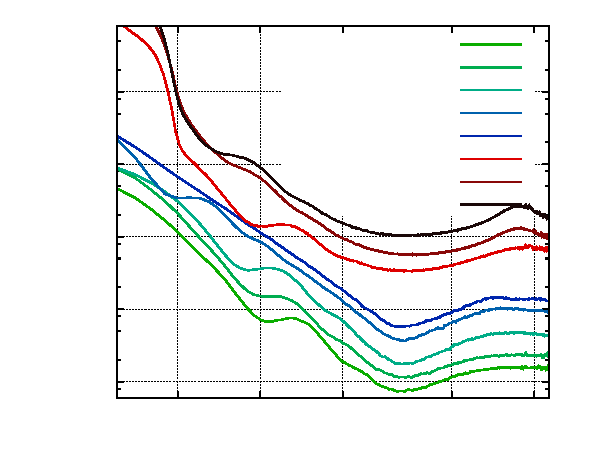
\includegraphics{SSLSingleContrast}}%
    \gplfronttext
  \end{picture}%
\endgroup

		\caption{Scattering curves of the different liposomes in buffer. The curves are intensity shifted for clarity. The 5 SSLs are presented in the lower part of the plot. The sizes in the legend are extracted form DLS measurements.}
		\label{fig:SSLSingleContrast}
\end{figure}

For this purpose, 5 PEGylated and 3 plain liposomes were extruded with different pore sizes, as explained in section \ref{sec:materials_SSL}. To simplify the following discussion, the liposomes are named after the hydrodynamic diameter measured by DLS. The SAXS measurements of the 8 liposomes are showed in figure \ref{fig:SSLSingleContrast}, where the first minimum shifts from $\sim$0.1 nm$^{-1}$ to smaller $q$-values for increasing size. For high polydispersities this scattering minimum gets smeared out, as it can be observed for the 274.1 nm SSL. It can be stated from these measurements and the DLS results that the polydispersity degree rises for increasing liposomal sizes. Besides, non-PEGylated liposomes show slightly broader size distributions than SSLs.

\begin{figure}
	\centering
		% GNUPLOT: LaTeX picture with Postscript
\begingroup
  \makeatletter
  \providecommand\color[2][]{%
    \GenericError{(gnuplot) \space\space\space\@spaces}{%
      Package color not loaded in conjunction with
      terminal option `colourtext'%
    }{See the gnuplot documentation for explanation.%
    }{Either use 'blacktext' in gnuplot or load the package
      color.sty in LaTeX.}%
    \renewcommand\color[2][]{}%
  }%
  \providecommand\includegraphics[2][]{%
    \GenericError{(gnuplot) \space\space\space\@spaces}{%
      Package graphicx or graphics not loaded%
    }{See the gnuplot documentation for explanation.%
    }{The gnuplot epslatex terminal needs graphicx.sty or graphics.sty.}%
    \renewcommand\includegraphics[2][]{}%
  }%
  \providecommand\rotatebox[2]{#2}%
  \@ifundefined{ifGPcolor}{%
    \newif\ifGPcolor
    \GPcolortrue
  }{}%
  \@ifundefined{ifGPblacktext}{%
    \newif\ifGPblacktext
    \GPblacktextfalse
  }{}%
  % define a \g@addto@macro without @ in the name:
  \let\gplgaddtomacro\g@addto@macro
  % define empty templates for all commands taking text:
  \gdef\gplbacktext{}%
  \gdef\gplfronttext{}%
  \makeatother
  \ifGPblacktext
    % no textcolor at all
    \def\colorrgb#1{}%
    \def\colorgray#1{}%
  \else
    % gray or color?
    \ifGPcolor
      \def\colorrgb#1{\color[rgb]{#1}}%
      \def\colorgray#1{\color[gray]{#1}}%
      \expandafter\def\csname LTw\endcsname{\color{white}}%
      \expandafter\def\csname LTb\endcsname{\color{black}}%
      \expandafter\def\csname LTa\endcsname{\color{black}}%
      \expandafter\def\csname LT0\endcsname{\color[rgb]{1,0,0}}%
      \expandafter\def\csname LT1\endcsname{\color[rgb]{0,1,0}}%
      \expandafter\def\csname LT2\endcsname{\color[rgb]{0,0,1}}%
      \expandafter\def\csname LT3\endcsname{\color[rgb]{1,0,1}}%
      \expandafter\def\csname LT4\endcsname{\color[rgb]{0,1,1}}%
      \expandafter\def\csname LT5\endcsname{\color[rgb]{1,1,0}}%
      \expandafter\def\csname LT6\endcsname{\color[rgb]{0,0,0}}%
      \expandafter\def\csname LT7\endcsname{\color[rgb]{1,0.3,0}}%
      \expandafter\def\csname LT8\endcsname{\color[rgb]{0.5,0.5,0.5}}%
    \else
      % gray
      \def\colorrgb#1{\color{black}}%
      \def\colorgray#1{\color[gray]{#1}}%
      \expandafter\def\csname LTw\endcsname{\color{white}}%
      \expandafter\def\csname LTb\endcsname{\color{black}}%
      \expandafter\def\csname LTa\endcsname{\color{black}}%
      \expandafter\def\csname LT0\endcsname{\color{black}}%
      \expandafter\def\csname LT1\endcsname{\color{black}}%
      \expandafter\def\csname LT2\endcsname{\color{black}}%
      \expandafter\def\csname LT3\endcsname{\color{black}}%
      \expandafter\def\csname LT4\endcsname{\color{black}}%
      \expandafter\def\csname LT5\endcsname{\color{black}}%
      \expandafter\def\csname LT6\endcsname{\color{black}}%
      \expandafter\def\csname LT7\endcsname{\color{black}}%
      \expandafter\def\csname LT8\endcsname{\color{black}}%
    \fi
  \fi
  \setlength{\unitlength}{0.0500bp}%
  \begin{picture}(3968.00,6236.00)%
    \gplgaddtomacro\gplbacktext{%
      \csname LTb\endcsname%
      \put(726,1118){\makebox(0,0)[r]{\strut{} 1}}%
      \csname LTb\endcsname%
      \put(726,2983){\makebox(0,0)[r]{\strut{} 10}}%
      \csname LTb\endcsname%
      \put(726,4848){\makebox(0,0)[r]{\strut{} 100}}%
      \csname LTb\endcsname%
      \put(1413,484){\makebox(0,0){\strut{} 0.5}}%
      \csname LTb\endcsname%
      \put(2492,484){\makebox(0,0){\strut{} 1}}%
      \csname LTb\endcsname%
      \put(3571,484){\makebox(0,0){\strut{} 2}}%
      \put(220,3117){\rotatebox{-270}{\makebox(0,0){\strut{}Scattering Intensity / a.u.}}}%
      \put(2214,154){\makebox(0,0){\strut{}$q$ / nm$^{-1}$}}%
    }%
    \gplgaddtomacro\gplfronttext{%
      \csname LTb\endcsname%
      \put(2584,5798){\makebox(0,0)[r]{\strut{}PEG 103 nm}}%
      \csname LTb\endcsname%
      \put(2584,5578){\makebox(0,0)[r]{\strut{}PEG 179 nm}}%
      \csname LTb\endcsname%
      \put(2584,5358){\makebox(0,0)[r]{\strut{}PEG 274 nm}}%
      \csname LTb\endcsname%
      \put(2584,5138){\makebox(0,0)[r]{\strut{}plain 89 nm}}%
      \csname LTb\endcsname%
      \put(2584,4918){\makebox(0,0)[r]{\strut{}plain 128 nm}}%
    }%
    \gplbacktext
    \put(0,0){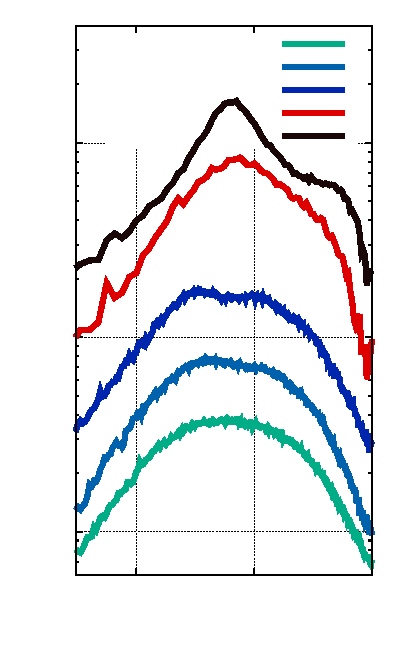
\includegraphics{SSLSingleContrastBilayer}}%
    \gplfronttext
  \end{picture}%
\endgroup

		\caption{The phospholipid bilayer feature: High $q$-region of the scattering curves of 2 plain liposomes and the 3 largest SSLs. The SSLs are presented in the lower part of the plot.}
		\label{fig:SSLSingleContrastBilayer}
\end{figure}

Focusing on the high $q$-region of the single-contrast SAXS curves as displayed in figure \ref{fig:SSLSingleContrastBilayer}, the scattering feature related to the phospholipid bilayer structure is observed. For Unilamellar Vesicles (ULV), the feature shape is typically round with a maximum around $q=0.86$ nm$^{-1}$ \cite{varga_characterization_2012}, related to a distance of 7.3 nm, as it can be seen in the case of small PEGylated liposomes. For SSLs extruded with larger pores, the bilayer shape shows incipient Bragg peaks which suggest the simultaneous presence of Multilamellar Vesicles (MLV) with unilamellar SSLs. Nevertheless, the MLV population cannot exceed 10 $\%$ of the total liposomes \cite{sakuragi_transformation_2011}, as the scattering contribution from ULV is still clearly dominant.

However, the bilayer feature of the plain liposomes differs completely from the round shape visible in unilamellar vesicles. The diffraction peaks appearing at $q_1=0.88$ and $q_2=1.9\simeq2q_1$ nm$^{-1}$ correspond to a slightly smaller lamellar repeat distance of 7.1 nm and the narrow shape of the bilayer feature indicates a variation of the phospholipid bilayer form factor. This change in the bilayer is emphasized for larger vesicles, as observed for the 127.7 plain liposome.

The effect of PEGylation induces a higher membrane stability due to the sterical stabilization of the liposome and the reduction of the electrostatic interactions within the phospholipid bilayer. The electrostatic repulsion in the non-PEGylated membrane is revealed by the appearance of the Bragg peaks in the plain liposomes. Nevertheless, secondary populations of MLVs coexisting with unilamellar liposomes can be observed for large extrusion pore sizes. In conclusion, the size and composition of the liposomes affect remarkably the formation of unilamellar vesicles and the shape of the phospholipid bilayer.

\begin{figure}
	\centering
		% GNUPLOT: LaTeX picture with Postscript
\begingroup
  \makeatletter
  \providecommand\color[2][]{%
    \GenericError{(gnuplot) \space\space\space\@spaces}{%
      Package color not loaded in conjunction with
      terminal option `colourtext'%
    }{See the gnuplot documentation for explanation.%
    }{Either use 'blacktext' in gnuplot or load the package
      color.sty in LaTeX.}%
    \renewcommand\color[2][]{}%
  }%
  \providecommand\includegraphics[2][]{%
    \GenericError{(gnuplot) \space\space\space\@spaces}{%
      Package graphicx or graphics not loaded%
    }{See the gnuplot documentation for explanation.%
    }{The gnuplot epslatex terminal needs graphicx.sty or graphics.sty.}%
    \renewcommand\includegraphics[2][]{}%
  }%
  \providecommand\rotatebox[2]{#2}%
  \@ifundefined{ifGPcolor}{%
    \newif\ifGPcolor
    \GPcolortrue
  }{}%
  \@ifundefined{ifGPblacktext}{%
    \newif\ifGPblacktext
    \GPblacktextfalse
  }{}%
  % define a \g@addto@macro without @ in the name:
  \let\gplgaddtomacro\g@addto@macro
  % define empty templates for all commands taking text:
  \gdef\gplbacktext{}%
  \gdef\gplfronttext{}%
  \makeatother
  \ifGPblacktext
    % no textcolor at all
    \def\colorrgb#1{}%
    \def\colorgray#1{}%
  \else
    % gray or color?
    \ifGPcolor
      \def\colorrgb#1{\color[rgb]{#1}}%
      \def\colorgray#1{\color[gray]{#1}}%
      \expandafter\def\csname LTw\endcsname{\color{white}}%
      \expandafter\def\csname LTb\endcsname{\color{black}}%
      \expandafter\def\csname LTa\endcsname{\color{black}}%
      \expandafter\def\csname LT0\endcsname{\color[rgb]{1,0,0}}%
      \expandafter\def\csname LT1\endcsname{\color[rgb]{0,1,0}}%
      \expandafter\def\csname LT2\endcsname{\color[rgb]{0,0,1}}%
      \expandafter\def\csname LT3\endcsname{\color[rgb]{1,0,1}}%
      \expandafter\def\csname LT4\endcsname{\color[rgb]{0,1,1}}%
      \expandafter\def\csname LT5\endcsname{\color[rgb]{1,1,0}}%
      \expandafter\def\csname LT6\endcsname{\color[rgb]{0,0,0}}%
      \expandafter\def\csname LT7\endcsname{\color[rgb]{1,0.3,0}}%
      \expandafter\def\csname LT8\endcsname{\color[rgb]{0.5,0.5,0.5}}%
    \else
      % gray
      \def\colorrgb#1{\color{black}}%
      \def\colorgray#1{\color[gray]{#1}}%
      \expandafter\def\csname LTw\endcsname{\color{white}}%
      \expandafter\def\csname LTb\endcsname{\color{black}}%
      \expandafter\def\csname LTa\endcsname{\color{black}}%
      \expandafter\def\csname LT0\endcsname{\color{black}}%
      \expandafter\def\csname LT1\endcsname{\color{black}}%
      \expandafter\def\csname LT2\endcsname{\color{black}}%
      \expandafter\def\csname LT3\endcsname{\color{black}}%
      \expandafter\def\csname LT4\endcsname{\color{black}}%
      \expandafter\def\csname LT5\endcsname{\color{black}}%
      \expandafter\def\csname LT6\endcsname{\color{black}}%
      \expandafter\def\csname LT7\endcsname{\color{black}}%
      \expandafter\def\csname LT8\endcsname{\color{black}}%
    \fi
  \fi
  \setlength{\unitlength}{0.0500bp}%
  \begin{picture}(5668.00,4534.00)%
    \gplgaddtomacro\gplbacktext{%
      \csname LTb\endcsname%
      \put(919,967){\makebox(0,0)[r]{\strut{} 1}}%
      \csname LTb\endcsname%
      \put(919,1841){\makebox(0,0)[r]{\strut{} 10}}%
      \csname LTb\endcsname%
      \put(919,2715){\makebox(0,0)[r]{\strut{} 100}}%
      \csname LTb\endcsname%
      \put(919,3589){\makebox(0,0)[r]{\strut{} 1000}}%
      \csname LTb\endcsname%
      \put(1528,484){\makebox(0,0){\strut{} 0.05}}%
      \csname LTb\endcsname%
      \put(2175,484){\makebox(0,0){\strut{} 0.1}}%
      \csname LTb\endcsname%
      \put(2822,484){\makebox(0,0){\strut{} 0.2}}%
      \csname LTb\endcsname%
      \put(3678,484){\makebox(0,0){\strut{} 0.5}}%
      \csname LTb\endcsname%
      \put(4325,484){\makebox(0,0){\strut{} 1}}%
      \put(176,2266){\rotatebox{-270}{\makebox(0,0){\strut{}Scattering Intensity / a.u.}}}%
      \put(2745,154){\makebox(0,0){\strut{}$q$ / nm$^{-1}$}}%
      \colorrgb{0.00,0.00,0.00}%
      \put(1842,1230){\makebox(0,0){\strut{}\smaller \shortstack{Pseudo\\Isoscattering\\Point}}}%
    }%
    \gplgaddtomacro\gplfronttext{%
      \csname LTb\endcsname%
      \put(4825,704){\makebox(0,0)[l]{\strut{}\smaller 0}}%
      \put(4825,1354){\makebox(0,0)[l]{\strut{}\smaller 5}}%
      \put(4825,2005){\makebox(0,0)[l]{\strut{}\smaller 10}}%
      \put(4825,2655){\makebox(0,0)[l]{\strut{}\smaller 15}}%
      \put(4825,3306){\makebox(0,0)[l]{\strut{}\smaller 20}}%
      \put(4825,3956){\makebox(0,0)[l]{\strut{}\smaller 25}}%
      \put(5222,2486){\rotatebox{-90}{\makebox(0,0){\strut{}\smaller Sucrose Mass Fraction / $\%$}}}%
    }%
    \gplbacktext
    \put(0,0){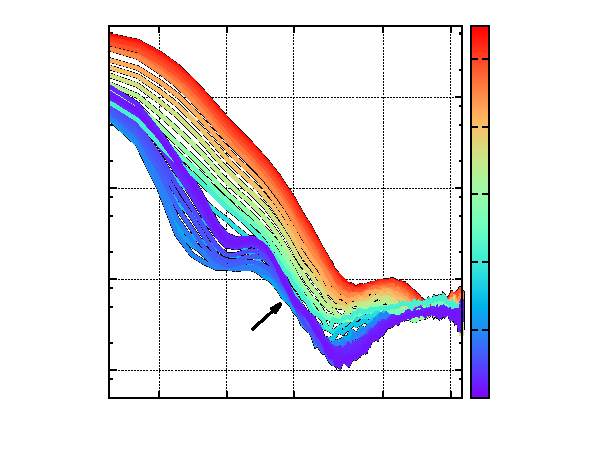
\includegraphics{SSLContinuousSAXS}}%
    \gplfronttext
  \end{picture}%
\endgroup

		\caption{Scattering curves of the 81.4 nm SSL measured at different solvent osmolalities with an aqueous sucrose density gradient. The position of the pseudo isoscattering point at $q=0.18$ nm$^{-1}$ is marked.}
		\label{fig:SSLContinuousSAXS}
\end{figure}

The behavior of the different liposomal structures to osmotic stress can be examined with a continuous contrast variation experiment using sucrose as contrast agent, similarly to the measurements with the Caelyx sample in section \ref{sec:OsmoticCaelyx}. The scattering curves measured for a PEGylated liposome with size 81.4 nm are displayed in figure \ref{fig:SSLContinuousSAXS}, where the solvent osmolality has been increased until 1409 mOsm kg$^{-1}$ using a maximum sucrose mass fraction of 27.3 $\%$. From the low $q$-region of these scattering curves some facts can be extracted which reveal preliminary the structural changes of the liposome induced by the osmotic pressure applied.

\begin{figure}
	\centering
		% GNUPLOT: LaTeX picture with Postscript
\begingroup
  \makeatletter
  \providecommand\color[2][]{%
    \GenericError{(gnuplot) \space\space\space\@spaces}{%
      Package color not loaded in conjunction with
      terminal option `colourtext'%
    }{See the gnuplot documentation for explanation.%
    }{Either use 'blacktext' in gnuplot or load the package
      color.sty in LaTeX.}%
    \renewcommand\color[2][]{}%
  }%
  \providecommand\includegraphics[2][]{%
    \GenericError{(gnuplot) \space\space\space\@spaces}{%
      Package graphicx or graphics not loaded%
    }{See the gnuplot documentation for explanation.%
    }{The gnuplot epslatex terminal needs graphicx.sty or graphics.sty.}%
    \renewcommand\includegraphics[2][]{}%
  }%
  \providecommand\rotatebox[2]{#2}%
  \@ifundefined{ifGPcolor}{%
    \newif\ifGPcolor
    \GPcolortrue
  }{}%
  \@ifundefined{ifGPblacktext}{%
    \newif\ifGPblacktext
    \GPblacktextfalse
  }{}%
  % define a \g@addto@macro without @ in the name:
  \let\gplgaddtomacro\g@addto@macro
  % define empty templates for all commands taking text:
  \gdef\gplbacktext{}%
  \gdef\gplfronttext{}%
  \makeatother
  \ifGPblacktext
    % no textcolor at all
    \def\colorrgb#1{}%
    \def\colorgray#1{}%
  \else
    % gray or color?
    \ifGPcolor
      \def\colorrgb#1{\color[rgb]{#1}}%
      \def\colorgray#1{\color[gray]{#1}}%
      \expandafter\def\csname LTw\endcsname{\color{white}}%
      \expandafter\def\csname LTb\endcsname{\color{black}}%
      \expandafter\def\csname LTa\endcsname{\color{black}}%
      \expandafter\def\csname LT0\endcsname{\color[rgb]{1,0,0}}%
      \expandafter\def\csname LT1\endcsname{\color[rgb]{0,1,0}}%
      \expandafter\def\csname LT2\endcsname{\color[rgb]{0,0,1}}%
      \expandafter\def\csname LT3\endcsname{\color[rgb]{1,0,1}}%
      \expandafter\def\csname LT4\endcsname{\color[rgb]{0,1,1}}%
      \expandafter\def\csname LT5\endcsname{\color[rgb]{1,1,0}}%
      \expandafter\def\csname LT6\endcsname{\color[rgb]{0,0,0}}%
      \expandafter\def\csname LT7\endcsname{\color[rgb]{1,0.3,0}}%
      \expandafter\def\csname LT8\endcsname{\color[rgb]{0.5,0.5,0.5}}%
    \else
      % gray
      \def\colorrgb#1{\color{black}}%
      \def\colorgray#1{\color[gray]{#1}}%
      \expandafter\def\csname LTw\endcsname{\color{white}}%
      \expandafter\def\csname LTb\endcsname{\color{black}}%
      \expandafter\def\csname LTa\endcsname{\color{black}}%
      \expandafter\def\csname LT0\endcsname{\color{black}}%
      \expandafter\def\csname LT1\endcsname{\color{black}}%
      \expandafter\def\csname LT2\endcsname{\color{black}}%
      \expandafter\def\csname LT3\endcsname{\color{black}}%
      \expandafter\def\csname LT4\endcsname{\color{black}}%
      \expandafter\def\csname LT5\endcsname{\color{black}}%
      \expandafter\def\csname LT6\endcsname{\color{black}}%
      \expandafter\def\csname LT7\endcsname{\color{black}}%
      \expandafter\def\csname LT8\endcsname{\color{black}}%
    \fi
  \fi
  \setlength{\unitlength}{0.0500bp}%
  \begin{picture}(5668.00,4534.00)%
    \gplgaddtomacro\gplbacktext{%
      \csname LTb\endcsname%
      \put(550,1088){\makebox(0,0)[r]{\strut{} 0}}%
      \csname LTb\endcsname%
      \put(550,1636){\makebox(0,0)[r]{\strut{} 1}}%
      \csname LTb\endcsname%
      \put(550,2185){\makebox(0,0)[r]{\strut{} 2}}%
      \csname LTb\endcsname%
      \put(550,2733){\makebox(0,0)[r]{\strut{} 3}}%
      \csname LTb\endcsname%
      \put(550,3282){\makebox(0,0)[r]{\strut{} 4}}%
      \csname LTb\endcsname%
      \put(550,3830){\makebox(0,0)[r]{\strut{} 5}}%
      \csname LTb\endcsname%
      \put(682,484){\makebox(0,0){\strut{} 0}}%
      \csname LTb\endcsname%
      \put(1829,484){\makebox(0,0){\strut{} 5}}%
      \csname LTb\endcsname%
      \put(2977,484){\makebox(0,0){\strut{} 10}}%
      \csname LTb\endcsname%
      \put(4124,484){\makebox(0,0){\strut{} 15}}%
      \csname LTb\endcsname%
      \put(5271,484){\makebox(0,0){\strut{} 20}}%
      \put(176,2486){\rotatebox{-270}{\makebox(0,0){\strut{}Deviation from $q^{\star}$ intensity / $\%$}}}%
      \put(2976,154){\makebox(0,0){\strut{}Sucrose Mass Fraction / $\%$}}%
    }%
    \gplgaddtomacro\gplfronttext{%
      \csname LTb\endcsname%
      \put(4284,4096){\makebox(0,0)[r]{\strut{}plain - 89 nm}}%
      \csname LTb\endcsname%
      \put(4284,3876){\makebox(0,0)[r]{\strut{}PEG - 87 nm}}%
    }%
    \gplbacktext
    \put(0,0){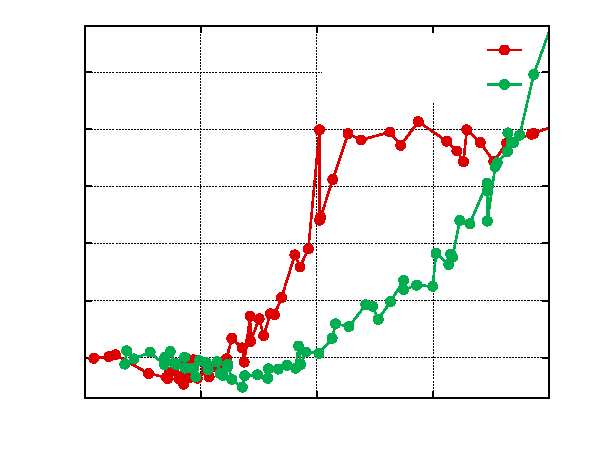
\includegraphics{SSLIsopointIntensity}}%
    \gplfronttext
  \end{picture}%
\endgroup

		\caption{Isoscattering point intensity: Deviation from the initial intensity at $q^{\star}$ at different solvent osmolalities measured for a PEGylated and plain liposome of similar sizes. A clear osmotic threshold can not be observed.}
		\label{fig:SSLIsopointIntensity}
\end{figure}

The curves do not intersect clearly in one point, even for low sucrose concentrations as occured in the Caelyx case. The absence of an evident isoscattering point can be related with the relatively high polydispersity of the sample or the shape variation of the liposome already at small osmotic pressures. However, a diffuse intersection point, or pseudo isoscattering point \cite{kawaguchi_application_2004}, is visible at $q=0.18$ nm$^{-1}$. In analogy to figure \ref{fig:CaelyxSucroseContinuousSAXSIsopoint}, the intensity of the pseudo $q^{\star}$ as a function of the solvent osmolality is depicted in figure \ref{fig:SSLIsopointIntensity}, where the deviation from the original intensity at $q^{\star}$ is shown for a plain and a PEGylated liposome.

The intensity at $q^{\star}$ starts diverging from the original value already at very low solvent osmolalitites and reflects the continuous change in shape or size of the liposome when increasing the osmotic pressure. This behavior occurs for both SSLs and plain liposomes and suggest that a sharp osmotic threshold, like in the Caelyx case, does not exist. Thus, the response of liposomes to osmotic pressure is steady and is already apparent at low osmolalities.

Besides, an evident variaton of the scattering curves below $q\leq0.3$ nm $^{-1}$ is observed in figure \ref{fig:SSLContinuousSAXS} when increasing the solvent osmolality. For example, the minimum originally appearing at 0.1 nm $^{-1}$ shifts slightly to larger $q$-values and dissappears almost completely for high sucrose concentrations. This variation of the form factor is directly related with the flattening of the liposomal shape observed with Freeze-fracture TEM \cite{varga_osmotic_2014}. Due to the increased osmotic activity, the original spherical liposome shrinks into an oblate spheroid. This hypothesis can be further explored by focusing on the scattering feature related to the phospholipid bilayer at the high $q$-region.

\begin{figure}
	\centering
		\subfloat[PEG 178.9 nm]{\resizebox{0.44\linewidth}{!}{% GNUPLOT: LaTeX picture with Postscript
\begingroup
  \makeatletter
  \providecommand\color[2][]{%
    \GenericError{(gnuplot) \space\space\space\@spaces}{%
      Package color not loaded in conjunction with
      terminal option `colourtext'%
    }{See the gnuplot documentation for explanation.%
    }{Either use 'blacktext' in gnuplot or load the package
      color.sty in LaTeX.}%
    \renewcommand\color[2][]{}%
  }%
  \providecommand\includegraphics[2][]{%
    \GenericError{(gnuplot) \space\space\space\@spaces}{%
      Package graphicx or graphics not loaded%
    }{See the gnuplot documentation for explanation.%
    }{The gnuplot epslatex terminal needs graphicx.sty or graphics.sty.}%
    \renewcommand\includegraphics[2][]{}%
  }%
  \providecommand\rotatebox[2]{#2}%
  \@ifundefined{ifGPcolor}{%
    \newif\ifGPcolor
    \GPcolortrue
  }{}%
  \@ifundefined{ifGPblacktext}{%
    \newif\ifGPblacktext
    \GPblacktextfalse
  }{}%
  % define a \g@addto@macro without @ in the name:
  \let\gplgaddtomacro\g@addto@macro
  % define empty templates for all commands taking text:
  \gdef\gplbacktext{}%
  \gdef\gplfronttext{}%
  \makeatother
  \ifGPblacktext
    % no textcolor at all
    \def\colorrgb#1{}%
    \def\colorgray#1{}%
  \else
    % gray or color?
    \ifGPcolor
      \def\colorrgb#1{\color[rgb]{#1}}%
      \def\colorgray#1{\color[gray]{#1}}%
      \expandafter\def\csname LTw\endcsname{\color{white}}%
      \expandafter\def\csname LTb\endcsname{\color{black}}%
      \expandafter\def\csname LTa\endcsname{\color{black}}%
      \expandafter\def\csname LT0\endcsname{\color[rgb]{1,0,0}}%
      \expandafter\def\csname LT1\endcsname{\color[rgb]{0,1,0}}%
      \expandafter\def\csname LT2\endcsname{\color[rgb]{0,0,1}}%
      \expandafter\def\csname LT3\endcsname{\color[rgb]{1,0,1}}%
      \expandafter\def\csname LT4\endcsname{\color[rgb]{0,1,1}}%
      \expandafter\def\csname LT5\endcsname{\color[rgb]{1,1,0}}%
      \expandafter\def\csname LT6\endcsname{\color[rgb]{0,0,0}}%
      \expandafter\def\csname LT7\endcsname{\color[rgb]{1,0.3,0}}%
      \expandafter\def\csname LT8\endcsname{\color[rgb]{0.5,0.5,0.5}}%
    \else
      % gray
      \def\colorrgb#1{\color{black}}%
      \def\colorgray#1{\color[gray]{#1}}%
      \expandafter\def\csname LTw\endcsname{\color{white}}%
      \expandafter\def\csname LTb\endcsname{\color{black}}%
      \expandafter\def\csname LTa\endcsname{\color{black}}%
      \expandafter\def\csname LT0\endcsname{\color{black}}%
      \expandafter\def\csname LT1\endcsname{\color{black}}%
      \expandafter\def\csname LT2\endcsname{\color{black}}%
      \expandafter\def\csname LT3\endcsname{\color{black}}%
      \expandafter\def\csname LT4\endcsname{\color{black}}%
      \expandafter\def\csname LT5\endcsname{\color{black}}%
      \expandafter\def\csname LT6\endcsname{\color{black}}%
      \expandafter\def\csname LT7\endcsname{\color{black}}%
      \expandafter\def\csname LT8\endcsname{\color{black}}%
    \fi
  \fi
  \setlength{\unitlength}{0.0500bp}%
  \begin{picture}(5102.00,10204.00)%
    \gplgaddtomacro\gplbacktext{%
      \csname LTb\endcsname%
      \put(726,1865){\makebox(0,0)[r]{\strut{} 0.2}}%
      \csname LTb\endcsname%
      \put(726,4335){\makebox(0,0)[r]{\strut{} 0.5}}%
      \csname LTb\endcsname%
      \put(726,6203){\makebox(0,0)[r]{\strut{} 1}}%
      \csname LTb\endcsname%
      \put(726,8071){\makebox(0,0)[r]{\strut{} 2}}%
      \csname LTb\endcsname%
      \put(1812,484){\makebox(0,0){\strut{} 0.5}}%
      \csname LTb\endcsname%
      \put(2765,484){\makebox(0,0){\strut{} 1}}%
      \csname LTb\endcsname%
      \put(3719,484){\makebox(0,0){\strut{} 2}}%
      \put(220,5101){\rotatebox{-270}{\makebox(0,0){\strut{}Scattering Intensity / a.u.}}}%
      \put(2384,154){\makebox(0,0){\strut{}$q$ / nm$^{-1}$}}%
    }%
    \gplgaddtomacro\gplfronttext{%
      \csname LTb\endcsname%
      \put(4271,704){\makebox(0,0)[l]{\strut{}\smaller 0}}%
      \put(4271,2463){\makebox(0,0)[l]{\strut{}\smaller 2}}%
      \put(4271,4222){\makebox(0,0)[l]{\strut{}\smaller 4}}%
      \put(4271,5981){\makebox(0,0)[l]{\strut{}\smaller 6}}%
      \put(4271,7740){\makebox(0,0)[l]{\strut{}\smaller 8}}%
      \put(4271,9499){\makebox(0,0)[l]{\strut{}\smaller 10}}%
      \put(4536,5321){\rotatebox{-90}{\makebox(0,0){\strut{}\smaller Sucrose Concentration / $\%$}}}%
    }%
    \gplbacktext
    \put(0,0){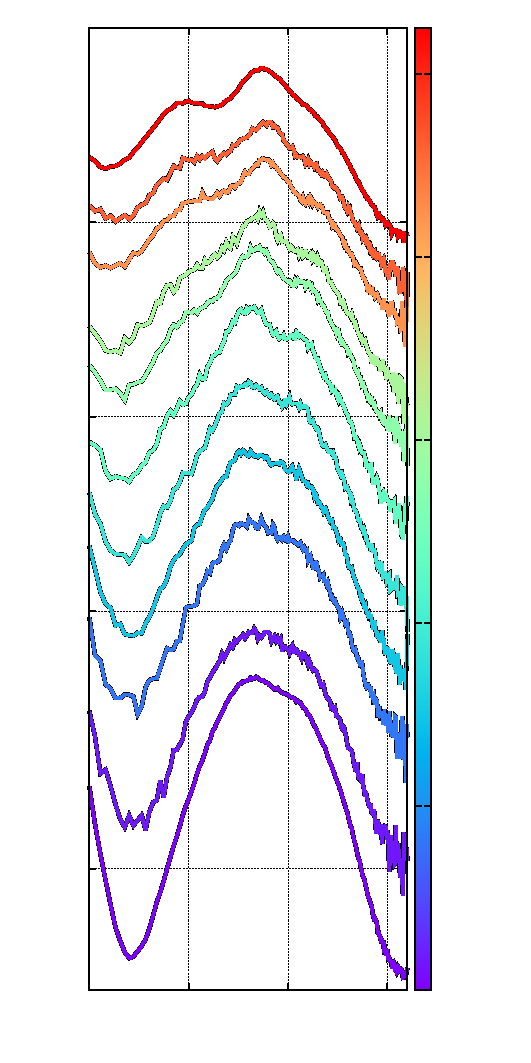
\includegraphics{SSLContrastCurvesBilayer200SSL}}%
    \gplfronttext
  \end{picture}%
\endgroup
}\label{fig:SSLContrastCurvesBilayer200SSL}}
		\subfloat[Plain 127.7 nm]{\resizebox{0.44\linewidth}{!}{% GNUPLOT: LaTeX picture with Postscript
\begingroup
  \makeatletter
  \providecommand\color[2][]{%
    \GenericError{(gnuplot) \space\space\space\@spaces}{%
      Package color not loaded in conjunction with
      terminal option `colourtext'%
    }{See the gnuplot documentation for explanation.%
    }{Either use 'blacktext' in gnuplot or load the package
      color.sty in LaTeX.}%
    \renewcommand\color[2][]{}%
  }%
  \providecommand\includegraphics[2][]{%
    \GenericError{(gnuplot) \space\space\space\@spaces}{%
      Package graphicx or graphics not loaded%
    }{See the gnuplot documentation for explanation.%
    }{The gnuplot epslatex terminal needs graphicx.sty or graphics.sty.}%
    \renewcommand\includegraphics[2][]{}%
  }%
  \providecommand\rotatebox[2]{#2}%
  \@ifundefined{ifGPcolor}{%
    \newif\ifGPcolor
    \GPcolortrue
  }{}%
  \@ifundefined{ifGPblacktext}{%
    \newif\ifGPblacktext
    \GPblacktextfalse
  }{}%
  % define a \g@addto@macro without @ in the name:
  \let\gplgaddtomacro\g@addto@macro
  % define empty templates for all commands taking text:
  \gdef\gplbacktext{}%
  \gdef\gplfronttext{}%
  \makeatother
  \ifGPblacktext
    % no textcolor at all
    \def\colorrgb#1{}%
    \def\colorgray#1{}%
  \else
    % gray or color?
    \ifGPcolor
      \def\colorrgb#1{\color[rgb]{#1}}%
      \def\colorgray#1{\color[gray]{#1}}%
      \expandafter\def\csname LTw\endcsname{\color{white}}%
      \expandafter\def\csname LTb\endcsname{\color{black}}%
      \expandafter\def\csname LTa\endcsname{\color{black}}%
      \expandafter\def\csname LT0\endcsname{\color[rgb]{1,0,0}}%
      \expandafter\def\csname LT1\endcsname{\color[rgb]{0,1,0}}%
      \expandafter\def\csname LT2\endcsname{\color[rgb]{0,0,1}}%
      \expandafter\def\csname LT3\endcsname{\color[rgb]{1,0,1}}%
      \expandafter\def\csname LT4\endcsname{\color[rgb]{0,1,1}}%
      \expandafter\def\csname LT5\endcsname{\color[rgb]{1,1,0}}%
      \expandafter\def\csname LT6\endcsname{\color[rgb]{0,0,0}}%
      \expandafter\def\csname LT7\endcsname{\color[rgb]{1,0.3,0}}%
      \expandafter\def\csname LT8\endcsname{\color[rgb]{0.5,0.5,0.5}}%
    \else
      % gray
      \def\colorrgb#1{\color{black}}%
      \def\colorgray#1{\color[gray]{#1}}%
      \expandafter\def\csname LTw\endcsname{\color{white}}%
      \expandafter\def\csname LTb\endcsname{\color{black}}%
      \expandafter\def\csname LTa\endcsname{\color{black}}%
      \expandafter\def\csname LT0\endcsname{\color{black}}%
      \expandafter\def\csname LT1\endcsname{\color{black}}%
      \expandafter\def\csname LT2\endcsname{\color{black}}%
      \expandafter\def\csname LT3\endcsname{\color{black}}%
      \expandafter\def\csname LT4\endcsname{\color{black}}%
      \expandafter\def\csname LT5\endcsname{\color{black}}%
      \expandafter\def\csname LT6\endcsname{\color{black}}%
      \expandafter\def\csname LT7\endcsname{\color{black}}%
      \expandafter\def\csname LT8\endcsname{\color{black}}%
    \fi
  \fi
    \setlength{\unitlength}{0.0500bp}%
    \ifx\gptboxheight\undefined%
      \newlength{\gptboxheight}%
      \newlength{\gptboxwidth}%
      \newsavebox{\gptboxtext}%
    \fi%
    \setlength{\fboxrule}{0.5pt}%
    \setlength{\fboxsep}{1pt}%
\begin{picture}(3968.00,6236.00)%
    \gplgaddtomacro\gplbacktext{%
      \csname LTb\endcsname%
      \put(594,1199){\makebox(0,0)[r]{\strut{}$1$}}%
      \csname LTb\endcsname%
      \put(594,2843){\makebox(0,0)[r]{\strut{}$10$}}%
      \csname LTb\endcsname%
      \put(594,4486){\makebox(0,0)[r]{\strut{}$100$}}%
      \csname LTb\endcsname%
      \put(1412,484){\makebox(0,0){\strut{}$0.5$}}%
      \csname LTb\endcsname%
      \put(2097,484){\makebox(0,0){\strut{}$1$}}%
      \csname LTb\endcsname%
      \put(2783,484){\makebox(0,0){\strut{}$2$}}%
    }%
    \gplgaddtomacro\gplfronttext{%
      \csname LTb\endcsname%
      \put(220,3117){\rotatebox{-270}{\makebox(0,0){\strut{}Scattering Intensity / a.u.}}}%
      \put(1801,154){\makebox(0,0){\strut{}$q$ / nm$^{-1}$}}%
      \csname LTb\endcsname%
      \put(3170,704){\makebox(0,0)[l]{\strut{}$0$}}%
      \put(3170,1757){\makebox(0,0)[l]{\strut{}$5$}}%
      \put(3170,2810){\makebox(0,0)[l]{\strut{}$10$}}%
      \put(3170,3864){\makebox(0,0)[l]{\strut{}$15$}}%
      \put(3170,4917){\makebox(0,0)[l]{\strut{}$20$}}%
      \put(3170,5971){\makebox(0,0)[l]{\strut{}$25$}}%
      \put(3369,3337){\rotatebox{-90}{\makebox(0,0){\strut{}Sucrose Concentration / $\%$}}}%
    }%
    \gplbacktext
    \put(0,0){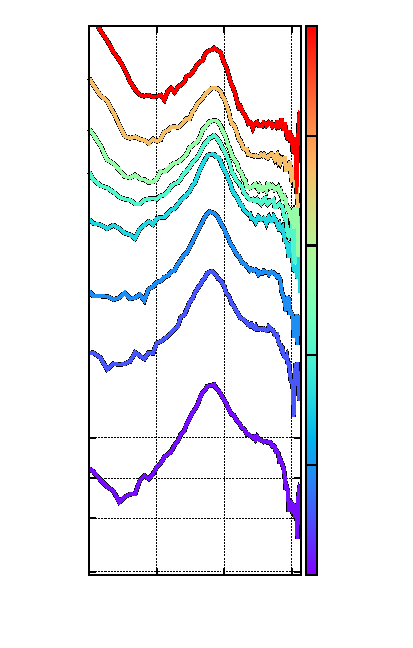
\includegraphics{SSLContrastCurvesBilayer100Plain}}%
    \gplfronttext
  \end{picture}%
\endgroup
}\label{fig:SSLContrastCurvesBilayer100Plain}}
		\caption{Osmotic effects in the phospholipid bilayer: Scattering curves measured at different solvent osmolalities for a 178.9 nm SSL and a 127.7 nm plain liposome. The appearance of Bragg peaks in the SSL membrane contrasts with the unaltered shape of the bilayer in the plain liposome.}
\end{figure}

For this purpose, the bilayer feature of the 178.9 nm PEGylated liposome is shown in figure \ref{fig:SSLContrastCurvesBilayer200SSL} for increasing solvent osmolalities. The scattering curves were measured with sucrose concentrations $\leq10\;\%$ to avoid undesired contrast effects, because the average electron density of the phospholipid bilayer is ca. 348 nm$^{-3}$, which corresponds to a sucrose mass fraction of $\sim 12 \; \%$. Indeed, the bilayer form factor shows undesired, large contrast effects for solvent densities close to the average density of the membrane, i.e. match point, as already observed in figure \ref{fig:SSLContinuousSAXS}, where the bilayer feature shifts abruptly to smaller $q$-values for sucrose concentrations above 15 $\%$. The convolution of the contrast-related effects with the variations induced by the osmotic pressure demands a more challenging evaluation, can prevent the right interpretation of the data and is, thus, unwanted.

The original double-peak structure of the SSL at 0 $\%$ sucrose concentration observed in figure \ref{fig:SSLContrastCurvesBilayer200SSL} transforms upon increasing the solvent osmolality and splits into 3 peaks of decreasing intensity at $q_1=0.48$ nm$^{-1}$, $q_2=0.86$ nm$^{-1}$ and $q_3=1.28$ nm$^{-1}$. These Bragg peaks superimposed on the bilayer form factor reveal a periodic structure which can be related with a partial oligolamellar structure in the liposome system \cite{fernandez_influence_2008}. The 3 mentioned diffraction peaks translate into a lamellar repeat distance of ca. 13 nm, approximately doubling the thickness of the single phospholipid bilayer \cite{kenworthy_range_1995} and suggesting the appearance of a bilamellar structure \cite{deme_giant_2002}. 

The transition between a single bilayer phase and a bilamellar phase at 10 $\%$ sucrose concentration supports the hypothesis already presented that the liposome shrinks into lens-shaped vesicles due to the osmotic pressure. The bilamellar structure might arise from the close bilayer contacts at the outest part of the elliptical liposomes, while the single bilayer conformation still remains dominant in the midsection of the liposomes. A similar morphology has been observed after the osmotic shrinkage of DPPC/DSPE-PEG$_{2000}$ vesicles \cite{terreno_osmotically_2009}. In fact, this behavior was identical for all 5 studied PEGylated liposomes, independent of their size. 

\begin{figure}
	\centering
		% GNUPLOT: LaTeX picture with Postscript
\begingroup
  \makeatletter
  \providecommand\color[2][]{%
    \GenericError{(gnuplot) \space\space\space\@spaces}{%
      Package color not loaded in conjunction with
      terminal option `colourtext'%
    }{See the gnuplot documentation for explanation.%
    }{Either use 'blacktext' in gnuplot or load the package
      color.sty in LaTeX.}%
    \renewcommand\color[2][]{}%
  }%
  \providecommand\includegraphics[2][]{%
    \GenericError{(gnuplot) \space\space\space\@spaces}{%
      Package graphicx or graphics not loaded%
    }{See the gnuplot documentation for explanation.%
    }{The gnuplot epslatex terminal needs graphicx.sty or graphics.sty.}%
    \renewcommand\includegraphics[2][]{}%
  }%
  \providecommand\rotatebox[2]{#2}%
  \@ifundefined{ifGPcolor}{%
    \newif\ifGPcolor
    \GPcolortrue
  }{}%
  \@ifundefined{ifGPblacktext}{%
    \newif\ifGPblacktext
    \GPblacktextfalse
  }{}%
  % define a \g@addto@macro without @ in the name:
  \let\gplgaddtomacro\g@addto@macro
  % define empty templates for all commands taking text:
  \gdef\gplbacktext{}%
  \gdef\gplfronttext{}%
  \makeatother
  \ifGPblacktext
    % no textcolor at all
    \def\colorrgb#1{}%
    \def\colorgray#1{}%
  \else
    % gray or color?
    \ifGPcolor
      \def\colorrgb#1{\color[rgb]{#1}}%
      \def\colorgray#1{\color[gray]{#1}}%
      \expandafter\def\csname LTw\endcsname{\color{white}}%
      \expandafter\def\csname LTb\endcsname{\color{black}}%
      \expandafter\def\csname LTa\endcsname{\color{black}}%
      \expandafter\def\csname LT0\endcsname{\color[rgb]{1,0,0}}%
      \expandafter\def\csname LT1\endcsname{\color[rgb]{0,1,0}}%
      \expandafter\def\csname LT2\endcsname{\color[rgb]{0,0,1}}%
      \expandafter\def\csname LT3\endcsname{\color[rgb]{1,0,1}}%
      \expandafter\def\csname LT4\endcsname{\color[rgb]{0,1,1}}%
      \expandafter\def\csname LT5\endcsname{\color[rgb]{1,1,0}}%
      \expandafter\def\csname LT6\endcsname{\color[rgb]{0,0,0}}%
      \expandafter\def\csname LT7\endcsname{\color[rgb]{1,0.3,0}}%
      \expandafter\def\csname LT8\endcsname{\color[rgb]{0.5,0.5,0.5}}%
    \else
      % gray
      \def\colorrgb#1{\color{black}}%
      \def\colorgray#1{\color[gray]{#1}}%
      \expandafter\def\csname LTw\endcsname{\color{white}}%
      \expandafter\def\csname LTb\endcsname{\color{black}}%
      \expandafter\def\csname LTa\endcsname{\color{black}}%
      \expandafter\def\csname LT0\endcsname{\color{black}}%
      \expandafter\def\csname LT1\endcsname{\color{black}}%
      \expandafter\def\csname LT2\endcsname{\color{black}}%
      \expandafter\def\csname LT3\endcsname{\color{black}}%
      \expandafter\def\csname LT4\endcsname{\color{black}}%
      \expandafter\def\csname LT5\endcsname{\color{black}}%
      \expandafter\def\csname LT6\endcsname{\color{black}}%
      \expandafter\def\csname LT7\endcsname{\color{black}}%
      \expandafter\def\csname LT8\endcsname{\color{black}}%
    \fi
  \fi
    \setlength{\unitlength}{0.0500bp}%
    \ifx\gptboxheight\undefined%
      \newlength{\gptboxheight}%
      \newlength{\gptboxwidth}%
      \newsavebox{\gptboxtext}%
    \fi%
    \setlength{\fboxrule}{0.5pt}%
    \setlength{\fboxsep}{1pt}%
\begin{picture}(5668.00,4534.00)%
    \gplgaddtomacro\gplbacktext{%
      \csname LTb\endcsname%
      \put(462,704){\makebox(0,0)[r]{\strut{}$0$}}%
      \csname LTb\endcsname%
      \put(462,1232){\makebox(0,0)[r]{\strut{}$2$}}%
      \csname LTb\endcsname%
      \put(462,1760){\makebox(0,0)[r]{\strut{}$4$}}%
      \csname LTb\endcsname%
      \put(462,2289){\makebox(0,0)[r]{\strut{}$6$}}%
      \csname LTb\endcsname%
      \put(462,2817){\makebox(0,0)[r]{\strut{}$8$}}%
      \csname LTb\endcsname%
      \put(462,3345){\makebox(0,0)[r]{\strut{}$10$}}%
      \csname LTb\endcsname%
      \put(462,3873){\makebox(0,0)[r]{\strut{}$12$}}%
      \csname LTb\endcsname%
      \put(594,484){\makebox(0,0){\strut{}$0$}}%
      \csname LTb\endcsname%
      \put(1144,484){\makebox(0,0){\strut{}$1$}}%
      \csname LTb\endcsname%
      \put(1694,484){\makebox(0,0){\strut{}$2$}}%
      \csname LTb\endcsname%
      \put(2245,484){\makebox(0,0){\strut{}$3$}}%
      \csname LTb\endcsname%
      \put(2795,484){\makebox(0,0){\strut{}$4$}}%
      \csname LTb\endcsname%
      \put(3345,484){\makebox(0,0){\strut{}$5$}}%
      \csname LTb\endcsname%
      \put(3895,484){\makebox(0,0){\strut{}$6$}}%
      \csname LTb\endcsname%
      \put(4446,484){\makebox(0,0){\strut{}$7$}}%
      \csname LTb\endcsname%
      \put(4996,484){\makebox(0,0){\strut{}$8$}}%
      \put(1249,4093){\makebox(0,0){\strut{}$350$}}%
      \put(2111,4093){\makebox(0,0){\strut{}$400$}}%
      \put(2972,4093){\makebox(0,0){\strut{}$450$}}%
      \put(3834,4093){\makebox(0,0){\strut{}$500$}}%
      \put(4696,4093){\makebox(0,0){\strut{}$550$}}%
    }%
    \gplgaddtomacro\gplfronttext{%
      \csname LTb\endcsname%
      \put(220,2288){\rotatebox{-270}{\makebox(0,0){\strut{}Normalized $\chi^2$}}}%
      \put(2932,154){\makebox(0,0){\strut{}Sucrose Mass Fraction / $\%$}}%
      \put(2932,4422){\makebox(0,0){\strut{}Solvent Osmolality / mOsm kg$^{-1}$}}%
    }%
    \gplbacktext
    \put(0,0){\includegraphics{SSLContrastVariationChiSquared400SSL}}%
    \gplfronttext
  \end{picture}%
\endgroup

		\caption{Variation of the 274.1 nm SSL bilayer scattering feature for increasing solvent osmolalities: normalized difference of the scattering curves at a certain sucrose concentration and in buffer. There are no sharp transitions, thus the osmotic effect is continuously modfying the bilayer structure.}
		\label{fig:SSLContrastVariationChiSquared400SSL}
\end{figure}

Besides, the changes of the phospholipid bilayer form factor are smooth upon increasing the osmotic pressure as shown in figure \ref{fig:SSLContrastVariationChiSquared400SSL}, where the bilayer feature scattering for increasing sucrose concentration is compared to the scattering curve of the SSL in buffer. This validates the observation from figure \ref{fig:SSLIsopointIntensity} and confirms that the increasing solvent osmotilality affects continuously the structure of the liposomes and not as abruptly as in the case of Caelyx.

Contrarily, the phospholipid bilayer of the plain liposomes remains invariable upon increasing the solvent osmolality until 1285 mOsm kg$^{-1}$, as displayed in figure \ref{fig:SSLContrastCurvesBilayer100Plain}. This suggests that the MLV structure of the non-PEGylated vesicles increase their resilience and the multiple phospholipid bilayers strengthens the elastic modulus of the liposome membrane.

The fact that the incorporation of PEG moieties influences already the preparation and formation of the liposomes prevents a proper comparison of the osmotic effects between SSLs and plain liposomes. In fact, the existence of MLVs for non-PEGylated liposomes acts as a limiting factor for the osmotic activity. This contrasts with the osmotic effects observed in SSLs already at low sucrose concentrations which shrinks the PEGylated liposomes into oblated ellipsoids. 

Although the chemical effect of sucrose on the SSL membrane can be discussed, previous studies in this subject \cite{kiselev_does_2003, kiselev_sucrose_2001, kiselev_sucrose_2001-1}, the large size of the sucrose molecule and similar results with other experiments performed with salt \cite{varga_osmotic_2014} validate this approach. The study of the osmotic activity of liposomes can be perfomed successfully using aqueous sucrose and shows very distinguishable effects for ULV (PEGylated liposomes) and MLV (plain liposomes).

%\begin{figure}
%	\centering
%		\subfloat[Scattering curves]{\resizebox{0.44\linewidth}{!}{% GNUPLOT: LaTeX picture with Postscript
\begingroup
  \makeatletter
  \providecommand\color[2][]{%
    \GenericError{(gnuplot) \space\space\space\@spaces}{%
      Package color not loaded in conjunction with
      terminal option `colourtext'%
    }{See the gnuplot documentation for explanation.%
    }{Either use 'blacktext' in gnuplot or load the package
      color.sty in LaTeX.}%
    \renewcommand\color[2][]{}%
  }%
  \providecommand\includegraphics[2][]{%
    \GenericError{(gnuplot) \space\space\space\@spaces}{%
      Package graphicx or graphics not loaded%
    }{See the gnuplot documentation for explanation.%
    }{The gnuplot epslatex terminal needs graphicx.sty or graphics.sty.}%
    \renewcommand\includegraphics[2][]{}%
  }%
  \providecommand\rotatebox[2]{#2}%
  \@ifundefined{ifGPcolor}{%
    \newif\ifGPcolor
    \GPcolortrue
  }{}%
  \@ifundefined{ifGPblacktext}{%
    \newif\ifGPblacktext
    \GPblacktextfalse
  }{}%
  % define a \g@addto@macro without @ in the name:
  \let\gplgaddtomacro\g@addto@macro
  % define empty templates for all commands taking text:
  \gdef\gplbacktext{}%
  \gdef\gplfronttext{}%
  \makeatother
  \ifGPblacktext
    % no textcolor at all
    \def\colorrgb#1{}%
    \def\colorgray#1{}%
  \else
    % gray or color?
    \ifGPcolor
      \def\colorrgb#1{\color[rgb]{#1}}%
      \def\colorgray#1{\color[gray]{#1}}%
      \expandafter\def\csname LTw\endcsname{\color{white}}%
      \expandafter\def\csname LTb\endcsname{\color{black}}%
      \expandafter\def\csname LTa\endcsname{\color{black}}%
      \expandafter\def\csname LT0\endcsname{\color[rgb]{1,0,0}}%
      \expandafter\def\csname LT1\endcsname{\color[rgb]{0,1,0}}%
      \expandafter\def\csname LT2\endcsname{\color[rgb]{0,0,1}}%
      \expandafter\def\csname LT3\endcsname{\color[rgb]{1,0,1}}%
      \expandafter\def\csname LT4\endcsname{\color[rgb]{0,1,1}}%
      \expandafter\def\csname LT5\endcsname{\color[rgb]{1,1,0}}%
      \expandafter\def\csname LT6\endcsname{\color[rgb]{0,0,0}}%
      \expandafter\def\csname LT7\endcsname{\color[rgb]{1,0.3,0}}%
      \expandafter\def\csname LT8\endcsname{\color[rgb]{0.5,0.5,0.5}}%
    \else
      % gray
      \def\colorrgb#1{\color{black}}%
      \def\colorgray#1{\color[gray]{#1}}%
      \expandafter\def\csname LTw\endcsname{\color{white}}%
      \expandafter\def\csname LTb\endcsname{\color{black}}%
      \expandafter\def\csname LTa\endcsname{\color{black}}%
      \expandafter\def\csname LT0\endcsname{\color{black}}%
      \expandafter\def\csname LT1\endcsname{\color{black}}%
      \expandafter\def\csname LT2\endcsname{\color{black}}%
      \expandafter\def\csname LT3\endcsname{\color{black}}%
      \expandafter\def\csname LT4\endcsname{\color{black}}%
      \expandafter\def\csname LT5\endcsname{\color{black}}%
      \expandafter\def\csname LT6\endcsname{\color{black}}%
      \expandafter\def\csname LT7\endcsname{\color{black}}%
      \expandafter\def\csname LT8\endcsname{\color{black}}%
    \fi
  \fi
    \setlength{\unitlength}{0.0500bp}%
    \ifx\gptboxheight\undefined%
      \newlength{\gptboxheight}%
      \newlength{\gptboxwidth}%
      \newsavebox{\gptboxtext}%
    \fi%
    \setlength{\fboxrule}{0.5pt}%
    \setlength{\fboxsep}{1pt}%
\begin{picture}(5668.00,4534.00)%
    \gplgaddtomacro\gplbacktext{%
      \csname LTb\endcsname%
      \put(880,1002){\makebox(0,0)[r]{\strut{}$1$}}%
      \csname LTb\endcsname%
      \put(880,1992){\makebox(0,0)[r]{\strut{}$10$}}%
      \csname LTb\endcsname%
      \put(880,2981){\makebox(0,0)[r]{\strut{}$100$}}%
      \csname LTb\endcsname%
      \put(880,3971){\makebox(0,0)[r]{\strut{}$1000$}}%
      \csname LTb\endcsname%
      \put(1613,484){\makebox(0,0){\strut{}$0.05$}}%
      \csname LTb\endcsname%
      \put(2429,484){\makebox(0,0){\strut{}$0.1$}}%
      \csname LTb\endcsname%
      \put(3244,484){\makebox(0,0){\strut{}$0.2$}}%
      \csname LTb\endcsname%
      \put(4322,484){\makebox(0,0){\strut{}$0.5$}}%
      \csname LTb\endcsname%
      \put(5138,484){\makebox(0,0){\strut{}$1$}}%
    }%
    \gplgaddtomacro\gplfronttext{%
      \csname LTb\endcsname%
      \put(176,2486){\rotatebox{-270}{\makebox(0,0){\strut{}Scattering Intensity / a.u.}}}%
      \put(3273,154){\makebox(0,0){\strut{}$q$ / nm$^{-1}$}}%
      \csname LTb\endcsname%
      \put(4284,4096){\makebox(0,0)[r]{\strut{}In buffer}}%
      \csname LTb\endcsname%
      \put(4284,3876){\makebox(0,0)[r]{\strut{}Max. osmolality}}%
    }%
    \gplbacktext
    \put(0,0){\includegraphics{SSLCurveFeatureComparison}}%
    \gplfronttext
  \end{picture}%
\endgroup
}\label{fig:SSLCurveFeatureComparison}}
%		\subfloat[Bilayer deformation]{\resizebox{0.44\linewidth}{!}{% GNUPLOT: LaTeX picture with Postscript
\begingroup
  \makeatletter
  \providecommand\color[2][]{%
    \GenericError{(gnuplot) \space\space\space\@spaces}{%
      Package color not loaded in conjunction with
      terminal option `colourtext'%
    }{See the gnuplot documentation for explanation.%
    }{Either use 'blacktext' in gnuplot or load the package
      color.sty in LaTeX.}%
    \renewcommand\color[2][]{}%
  }%
  \providecommand\includegraphics[2][]{%
    \GenericError{(gnuplot) \space\space\space\@spaces}{%
      Package graphicx or graphics not loaded%
    }{See the gnuplot documentation for explanation.%
    }{The gnuplot epslatex terminal needs graphicx.sty or graphics.sty.}%
    \renewcommand\includegraphics[2][]{}%
  }%
  \providecommand\rotatebox[2]{#2}%
  \@ifundefined{ifGPcolor}{%
    \newif\ifGPcolor
    \GPcolortrue
  }{}%
  \@ifundefined{ifGPblacktext}{%
    \newif\ifGPblacktext
    \GPblacktextfalse
  }{}%
  % define a \g@addto@macro without @ in the name:
  \let\gplgaddtomacro\g@addto@macro
  % define empty templates for all commands taking text:
  \gdef\gplbacktext{}%
  \gdef\gplfronttext{}%
  \makeatother
  \ifGPblacktext
    % no textcolor at all
    \def\colorrgb#1{}%
    \def\colorgray#1{}%
  \else
    % gray or color?
    \ifGPcolor
      \def\colorrgb#1{\color[rgb]{#1}}%
      \def\colorgray#1{\color[gray]{#1}}%
      \expandafter\def\csname LTw\endcsname{\color{white}}%
      \expandafter\def\csname LTb\endcsname{\color{black}}%
      \expandafter\def\csname LTa\endcsname{\color{black}}%
      \expandafter\def\csname LT0\endcsname{\color[rgb]{1,0,0}}%
      \expandafter\def\csname LT1\endcsname{\color[rgb]{0,1,0}}%
      \expandafter\def\csname LT2\endcsname{\color[rgb]{0,0,1}}%
      \expandafter\def\csname LT3\endcsname{\color[rgb]{1,0,1}}%
      \expandafter\def\csname LT4\endcsname{\color[rgb]{0,1,1}}%
      \expandafter\def\csname LT5\endcsname{\color[rgb]{1,1,0}}%
      \expandafter\def\csname LT6\endcsname{\color[rgb]{0,0,0}}%
      \expandafter\def\csname LT7\endcsname{\color[rgb]{1,0.3,0}}%
      \expandafter\def\csname LT8\endcsname{\color[rgb]{0.5,0.5,0.5}}%
    \else
      % gray
      \def\colorrgb#1{\color{black}}%
      \def\colorgray#1{\color[gray]{#1}}%
      \expandafter\def\csname LTw\endcsname{\color{white}}%
      \expandafter\def\csname LTb\endcsname{\color{black}}%
      \expandafter\def\csname LTa\endcsname{\color{black}}%
      \expandafter\def\csname LT0\endcsname{\color{black}}%
      \expandafter\def\csname LT1\endcsname{\color{black}}%
      \expandafter\def\csname LT2\endcsname{\color{black}}%
      \expandafter\def\csname LT3\endcsname{\color{black}}%
      \expandafter\def\csname LT4\endcsname{\color{black}}%
      \expandafter\def\csname LT5\endcsname{\color{black}}%
      \expandafter\def\csname LT6\endcsname{\color{black}}%
      \expandafter\def\csname LT7\endcsname{\color{black}}%
      \expandafter\def\csname LT8\endcsname{\color{black}}%
    \fi
  \fi
  \setlength{\unitlength}{0.0500bp}%
  \begin{picture}(5668.00,4534.00)%
    \gplgaddtomacro\gplbacktext{%
      \csname LTb\endcsname%
      \put(880,704){\makebox(0,0)[r]{\strut{} 0}}%
      \csname LTb\endcsname%
      \put(880,1298){\makebox(0,0)[r]{\strut{} 5}}%
      \csname LTb\endcsname%
      \put(880,1892){\makebox(0,0)[r]{\strut{} 10}}%
      \csname LTb\endcsname%
      \put(880,2487){\makebox(0,0)[r]{\strut{} 15}}%
      \csname LTb\endcsname%
      \put(880,3081){\makebox(0,0)[r]{\strut{} 20}}%
      \csname LTb\endcsname%
      \put(880,3675){\makebox(0,0)[r]{\strut{} 25}}%
      \csname LTb\endcsname%
      \put(880,4269){\makebox(0,0)[r]{\strut{} 30}}%
      \csname LTb\endcsname%
      \put(1012,484){\makebox(0,0){\strut{} 0}}%
      \csname LTb\endcsname%
      \put(1864,484){\makebox(0,0){\strut{} 5}}%
      \csname LTb\endcsname%
      \put(2716,484){\makebox(0,0){\strut{} 10}}%
      \csname LTb\endcsname%
      \put(3567,484){\makebox(0,0){\strut{} 15}}%
      \csname LTb\endcsname%
      \put(4419,484){\makebox(0,0){\strut{} 20}}%
      \csname LTb\endcsname%
      \put(5271,484){\makebox(0,0){\strut{} 25}}%
      \put(176,2486){\rotatebox{-270}{\makebox(0,0){\strut{}Normalized $\chi^2$}}}%
      \put(3273,154){\makebox(0,0){\strut{}Sucrose Mass Fraction / $\%$}}%
      \colorrgb{0.00,0.00,1.00}%
      \put(3567,2273){\makebox(0,0){\strut{}Bilayer}}%
      \put(3567,2053){\makebox(0,0){\strut{}Deformation}}%
    }%
    \gplgaddtomacro\gplfronttext{%
      \csname LTb\endcsname%
      \put(4284,4096){\makebox(0,0)[r]{\strut{}Diff. to SSL in buffer}}%
      \csname LTb\endcsname%
      \put(4284,3876){\makebox(0,0)[r]{\strut{}Diff. to SSL in max. osmolality}}%
    }%
    \gplbacktext
    \put(0,0){\includegraphics{SSLBilayerDeformationChi2}}%
    \gplfronttext
  \end{picture}%
\endgroup
}\label{fig:SSLBilayerDeformationChi2}}
%		\caption{Scattering curve of SSL 50 nm (Oct 2015) in aqueous buffer and at maximum concentration. The phospholipid bilayer feature appears at $q>0.3$ nm$^{-1}$ and changes drastically from one curve to the other. At the right, the bilayer deformation is observed for increasing sucrose mass fraction e.g. solvent osmolality.}
%\end{figure}


%\begin{figure}
%	\centering
%		\subfloat[Poisson Law]{\resizebox{0.44\linewidth}{!}{% GNUPLOT: LaTeX picture with Postscript
\begingroup
  \makeatletter
  \providecommand\color[2][]{%
    \GenericError{(gnuplot) \space\space\space\@spaces}{%
      Package color not loaded in conjunction with
      terminal option `colourtext'%
    }{See the gnuplot documentation for explanation.%
    }{Either use 'blacktext' in gnuplot or load the package
      color.sty in LaTeX.}%
    \renewcommand\color[2][]{}%
  }%
  \providecommand\includegraphics[2][]{%
    \GenericError{(gnuplot) \space\space\space\@spaces}{%
      Package graphicx or graphics not loaded%
    }{See the gnuplot documentation for explanation.%
    }{The gnuplot epslatex terminal needs graphicx.sty or graphics.sty.}%
    \renewcommand\includegraphics[2][]{}%
  }%
  \providecommand\rotatebox[2]{#2}%
  \@ifundefined{ifGPcolor}{%
    \newif\ifGPcolor
    \GPcolortrue
  }{}%
  \@ifundefined{ifGPblacktext}{%
    \newif\ifGPblacktext
    \GPblacktextfalse
  }{}%
  % define a \g@addto@macro without @ in the name:
  \let\gplgaddtomacro\g@addto@macro
  % define empty templates for all commands taking text:
  \gdef\gplbacktext{}%
  \gdef\gplfronttext{}%
  \makeatother
  \ifGPblacktext
    % no textcolor at all
    \def\colorrgb#1{}%
    \def\colorgray#1{}%
  \else
    % gray or color?
    \ifGPcolor
      \def\colorrgb#1{\color[rgb]{#1}}%
      \def\colorgray#1{\color[gray]{#1}}%
      \expandafter\def\csname LTw\endcsname{\color{white}}%
      \expandafter\def\csname LTb\endcsname{\color{black}}%
      \expandafter\def\csname LTa\endcsname{\color{black}}%
      \expandafter\def\csname LT0\endcsname{\color[rgb]{1,0,0}}%
      \expandafter\def\csname LT1\endcsname{\color[rgb]{0,1,0}}%
      \expandafter\def\csname LT2\endcsname{\color[rgb]{0,0,1}}%
      \expandafter\def\csname LT3\endcsname{\color[rgb]{1,0,1}}%
      \expandafter\def\csname LT4\endcsname{\color[rgb]{0,1,1}}%
      \expandafter\def\csname LT5\endcsname{\color[rgb]{1,1,0}}%
      \expandafter\def\csname LT6\endcsname{\color[rgb]{0,0,0}}%
      \expandafter\def\csname LT7\endcsname{\color[rgb]{1,0.3,0}}%
      \expandafter\def\csname LT8\endcsname{\color[rgb]{0.5,0.5,0.5}}%
    \else
      % gray
      \def\colorrgb#1{\color{black}}%
      \def\colorgray#1{\color[gray]{#1}}%
      \expandafter\def\csname LTw\endcsname{\color{white}}%
      \expandafter\def\csname LTb\endcsname{\color{black}}%
      \expandafter\def\csname LTa\endcsname{\color{black}}%
      \expandafter\def\csname LT0\endcsname{\color{black}}%
      \expandafter\def\csname LT1\endcsname{\color{black}}%
      \expandafter\def\csname LT2\endcsname{\color{black}}%
      \expandafter\def\csname LT3\endcsname{\color{black}}%
      \expandafter\def\csname LT4\endcsname{\color{black}}%
      \expandafter\def\csname LT5\endcsname{\color{black}}%
      \expandafter\def\csname LT6\endcsname{\color{black}}%
      \expandafter\def\csname LT7\endcsname{\color{black}}%
      \expandafter\def\csname LT8\endcsname{\color{black}}%
    \fi
  \fi
    \setlength{\unitlength}{0.0500bp}%
    \ifx\gptboxheight\undefined%
      \newlength{\gptboxheight}%
      \newlength{\gptboxwidth}%
      \newsavebox{\gptboxtext}%
    \fi%
    \setlength{\fboxrule}{0.5pt}%
    \setlength{\fboxsep}{1pt}%
\begin{picture}(5668.00,4534.00)%
    \gplgaddtomacro\gplbacktext{%
      \csname LTb\endcsname%
      \put(880,704){\makebox(0,0)[r]{\strut{}$180$}}%
      \csname LTb\endcsname%
      \put(880,1150){\makebox(0,0)[r]{\strut{}$190$}}%
      \csname LTb\endcsname%
      \put(880,1595){\makebox(0,0)[r]{\strut{}$200$}}%
      \csname LTb\endcsname%
      \put(880,2041){\makebox(0,0)[r]{\strut{}$210$}}%
      \csname LTb\endcsname%
      \put(880,2487){\makebox(0,0)[r]{\strut{}$220$}}%
      \csname LTb\endcsname%
      \put(880,2932){\makebox(0,0)[r]{\strut{}$230$}}%
      \csname LTb\endcsname%
      \put(880,3378){\makebox(0,0)[r]{\strut{}$240$}}%
      \csname LTb\endcsname%
      \put(880,3823){\makebox(0,0)[r]{\strut{}$250$}}%
      \csname LTb\endcsname%
      \put(880,4269){\makebox(0,0)[r]{\strut{}$260$}}%
      \csname LTb\endcsname%
      \put(1012,484){\makebox(0,0){\strut{}$0.019$}}%
      \csname LTb\endcsname%
      \put(1722,484){\makebox(0,0){\strut{}$0.02$}}%
      \csname LTb\endcsname%
      \put(2432,484){\makebox(0,0){\strut{}$0.021$}}%
      \csname LTb\endcsname%
      \put(3142,484){\makebox(0,0){\strut{}$0.022$}}%
      \csname LTb\endcsname%
      \put(3851,484){\makebox(0,0){\strut{}$0.023$}}%
      \csname LTb\endcsname%
      \put(4561,484){\makebox(0,0){\strut{}$0.024$}}%
      \csname LTb\endcsname%
      \put(5271,484){\makebox(0,0){\strut{}$0.025$}}%
    }%
    \gplgaddtomacro\gplfronttext{%
      \csname LTb\endcsname%
      \put(176,2486){\rotatebox{-270}{\makebox(0,0){\strut{}Pressure difference / mOsm kg$^{-1}$}}}%
      \put(3273,154){\makebox(0,0){\strut{}1/Radius / nm$^{-1}$}}%
    }%
    \gplbacktext
    \put(0,0){\includegraphics{SSLPoissonOsmoticShrinkage}}%
    \gplfronttext
  \end{picture}%
\endgroup
}\label{fig:SSLPoissonOsmoticShrinkage}}
%		\subfloat[Bilayer deformation and osmotic shrinkage]{\resizebox{0.44\linewidth}{!}{% GNUPLOT: LaTeX picture with Postscript
\begingroup
  \makeatletter
  \providecommand\color[2][]{%
    \GenericError{(gnuplot) \space\space\space\@spaces}{%
      Package color not loaded in conjunction with
      terminal option `colourtext'%
    }{See the gnuplot documentation for explanation.%
    }{Either use 'blacktext' in gnuplot or load the package
      color.sty in LaTeX.}%
    \renewcommand\color[2][]{}%
  }%
  \providecommand\includegraphics[2][]{%
    \GenericError{(gnuplot) \space\space\space\@spaces}{%
      Package graphicx or graphics not loaded%
    }{See the gnuplot documentation for explanation.%
    }{The gnuplot epslatex terminal needs graphicx.sty or graphics.sty.}%
    \renewcommand\includegraphics[2][]{}%
  }%
  \providecommand\rotatebox[2]{#2}%
  \@ifundefined{ifGPcolor}{%
    \newif\ifGPcolor
    \GPcolortrue
  }{}%
  \@ifundefined{ifGPblacktext}{%
    \newif\ifGPblacktext
    \GPblacktextfalse
  }{}%
  % define a \g@addto@macro without @ in the name:
  \let\gplgaddtomacro\g@addto@macro
  % define empty templates for all commands taking text:
  \gdef\gplbacktext{}%
  \gdef\gplfronttext{}%
  \makeatother
  \ifGPblacktext
    % no textcolor at all
    \def\colorrgb#1{}%
    \def\colorgray#1{}%
  \else
    % gray or color?
    \ifGPcolor
      \def\colorrgb#1{\color[rgb]{#1}}%
      \def\colorgray#1{\color[gray]{#1}}%
      \expandafter\def\csname LTw\endcsname{\color{white}}%
      \expandafter\def\csname LTb\endcsname{\color{black}}%
      \expandafter\def\csname LTa\endcsname{\color{black}}%
      \expandafter\def\csname LT0\endcsname{\color[rgb]{1,0,0}}%
      \expandafter\def\csname LT1\endcsname{\color[rgb]{0,1,0}}%
      \expandafter\def\csname LT2\endcsname{\color[rgb]{0,0,1}}%
      \expandafter\def\csname LT3\endcsname{\color[rgb]{1,0,1}}%
      \expandafter\def\csname LT4\endcsname{\color[rgb]{0,1,1}}%
      \expandafter\def\csname LT5\endcsname{\color[rgb]{1,1,0}}%
      \expandafter\def\csname LT6\endcsname{\color[rgb]{0,0,0}}%
      \expandafter\def\csname LT7\endcsname{\color[rgb]{1,0.3,0}}%
      \expandafter\def\csname LT8\endcsname{\color[rgb]{0.5,0.5,0.5}}%
    \else
      % gray
      \def\colorrgb#1{\color{black}}%
      \def\colorgray#1{\color[gray]{#1}}%
      \expandafter\def\csname LTw\endcsname{\color{white}}%
      \expandafter\def\csname LTb\endcsname{\color{black}}%
      \expandafter\def\csname LTa\endcsname{\color{black}}%
      \expandafter\def\csname LT0\endcsname{\color{black}}%
      \expandafter\def\csname LT1\endcsname{\color{black}}%
      \expandafter\def\csname LT2\endcsname{\color{black}}%
      \expandafter\def\csname LT3\endcsname{\color{black}}%
      \expandafter\def\csname LT4\endcsname{\color{black}}%
      \expandafter\def\csname LT5\endcsname{\color{black}}%
      \expandafter\def\csname LT6\endcsname{\color{black}}%
      \expandafter\def\csname LT7\endcsname{\color{black}}%
      \expandafter\def\csname LT8\endcsname{\color{black}}%
    \fi
  \fi
  \setlength{\unitlength}{0.0500bp}%
  \begin{picture}(5668.00,4534.00)%
    \gplgaddtomacro\gplbacktext{%
      \csname LTb\endcsname%
      \put(1012,1014){\makebox(0,0)[r]{\strut{} 200}}%
      \csname LTb\endcsname%
      \put(1012,1402){\makebox(0,0)[r]{\strut{} 250}}%
      \csname LTb\endcsname%
      \put(1012,1789){\makebox(0,0)[r]{\strut{} 300}}%
      \csname LTb\endcsname%
      \put(1012,2177){\makebox(0,0)[r]{\strut{} 350}}%
      \csname LTb\endcsname%
      \put(1012,2564){\makebox(0,0)[r]{\strut{} 400}}%
      \csname LTb\endcsname%
      \put(1012,2952){\makebox(0,0)[r]{\strut{} 450}}%
      \csname LTb\endcsname%
      \put(1012,3339){\makebox(0,0)[r]{\strut{} 500}}%
      \csname LTb\endcsname%
      \put(1012,3727){\makebox(0,0)[r]{\strut{} 550}}%
      \csname LTb\endcsname%
      \put(1012,4114){\makebox(0,0)[r]{\strut{} 600}}%
      \csname LTb\endcsname%
      \put(1144,484){\makebox(0,0){\strut{} 0.014}}%
      \csname LTb\endcsname%
      \put(1894,484){\makebox(0,0){\strut{} 0.016}}%
      \csname LTb\endcsname%
      \put(2645,484){\makebox(0,0){\strut{} 0.018}}%
      \csname LTb\endcsname%
      \put(3395,484){\makebox(0,0){\strut{} 0.02}}%
      \csname LTb\endcsname%
      \put(4145,484){\makebox(0,0){\strut{} 0.022}}%
      \csname LTb\endcsname%
      \put(4896,484){\makebox(0,0){\strut{} 0.024}}%
      \put(176,2486){\rotatebox{-270}{\makebox(0,0){\strut{}Pressure difference / mOsm kg$^{-1}$}}}%
      \put(3339,154){\makebox(0,0){\strut{}1/Radius / nm$^{-1}$}}%
      \colorrgb{0.00,0.00,0.00}%
      \put(2270,1324){\makebox(0,0)[l]{\strut{}Osmotic Shrinkage}}%
      \colorrgb{0.80,0.31,0.31}%
      \put(3770,3107){\makebox(0,0)[l]{\strut{}HSPC+PEG}}%
      \colorrgb{0.43,0.42,0.82}%
      \put(1894,3727){\makebox(0,0)[l]{\strut{}HSPC}}%
      \colorrgb{0.00,0.00,0.00}%
      \put(3770,2254){\makebox(0,0)[l]{\strut{}Caelyx}}%
    }%
    \gplgaddtomacro\gplfronttext{%
    }%
    \gplbacktext
    \put(0,0){\includegraphics{SSLPoissonComplete}}%
    \gplfronttext
  \end{picture}%
\endgroup
}\label{fig:SSLPoissonComplete}}
%		\caption{Summary of the different osmotic pressures needed for the deformation of the liposamal structure. The radius was determined by DLS.}
%\end{figure}


\section{Application to blood plasma componenents}

From a nanoscience point of view, human blood can be seen as a suspension of particles with different physiological roles. Serum lipoproteins are the colloidal particles involved in the transport and metabolism of insoluble lipids and are among the most studied biological particles. The interest in their activity is understandable due to their direct relationship with very extended diseases in the Western world population, such as morbidity or atherogenesis, e.g. obturation of the arterial walls. For example, the dysregulation of cholesterol in plasma, primarly carried within lipoproteins, is responsible of atherosclerosis \cite{munro_pathogenesis_1988}. Besides, they are a convenient model for lipid-protein interactions \cite{assmann_lipid-protein_1974} due to their lipid core and the hydrated proteins isometrically situated on its surface.

Lipoproteins are normally classified by the density range within they are isolated from blood plasma by ultracentrifugation \cite{havel_distribution_1955}, showing different chemical composition, size and pathological condition for each class \cite{german_lipoproteins:_2006}. Indeed, the size of lipoproteins is critically connected with disease risk \cite{gardner_cd_association_1996} and Low-density Lipoproteins (LDL) are suggested to be more or less atherogenic depending on their size \cite{dreon_low-density_1994}. The effect of diabetes on the lipoprotein size is also of great interest, specially the sex-dependency of High-density Lipoproteins (HDL) size \cite{colhoun_lipoprotein_2002}.

Therefore, precise sizing techniques are a crucial tool to understand the physiological processes of lipoproteins \cite{german_lipoproteins:_2006}. The naturally narrow size distributions of LDL and HDL suggest small-angle scattering as a well-suited method and their heterogenous morphology advises the use of a contrast variation approach. For instance, the first characterization attempts date back to the late 1970s with neutron scattering \cite{stuhrmann_neutron_1975}, using salt \cite{tardieu_structure_1976} and sucrose \cite{muller_structure_1978} as SAXS contrast agents or modifying the sample temperature \cite{laggner_molecular_1977,luzzati_structure_1979}. 

\begin{figure}
	\centering
		\subfloat[HDL]{\resizebox{0.44\linewidth}{!}{% GNUPLOT: LaTeX picture with Postscript
\begingroup
  \makeatletter
  \providecommand\color[2][]{%
    \GenericError{(gnuplot) \space\space\space\@spaces}{%
      Package color not loaded in conjunction with
      terminal option `colourtext'%
    }{See the gnuplot documentation for explanation.%
    }{Either use 'blacktext' in gnuplot or load the package
      color.sty in LaTeX.}%
    \renewcommand\color[2][]{}%
  }%
  \providecommand\includegraphics[2][]{%
    \GenericError{(gnuplot) \space\space\space\@spaces}{%
      Package graphicx or graphics not loaded%
    }{See the gnuplot documentation for explanation.%
    }{The gnuplot epslatex terminal needs graphicx.sty or graphics.sty.}%
    \renewcommand\includegraphics[2][]{}%
  }%
  \providecommand\rotatebox[2]{#2}%
  \@ifundefined{ifGPcolor}{%
    \newif\ifGPcolor
    \GPcolortrue
  }{}%
  \@ifundefined{ifGPblacktext}{%
    \newif\ifGPblacktext
    \GPblacktextfalse
  }{}%
  % define a \g@addto@macro without @ in the name:
  \let\gplgaddtomacro\g@addto@macro
  % define empty templates for all commands taking text:
  \gdef\gplbacktext{}%
  \gdef\gplfronttext{}%
  \makeatother
  \ifGPblacktext
    % no textcolor at all
    \def\colorrgb#1{}%
    \def\colorgray#1{}%
  \else
    % gray or color?
    \ifGPcolor
      \def\colorrgb#1{\color[rgb]{#1}}%
      \def\colorgray#1{\color[gray]{#1}}%
      \expandafter\def\csname LTw\endcsname{\color{white}}%
      \expandafter\def\csname LTb\endcsname{\color{black}}%
      \expandafter\def\csname LTa\endcsname{\color{black}}%
      \expandafter\def\csname LT0\endcsname{\color[rgb]{1,0,0}}%
      \expandafter\def\csname LT1\endcsname{\color[rgb]{0,1,0}}%
      \expandafter\def\csname LT2\endcsname{\color[rgb]{0,0,1}}%
      \expandafter\def\csname LT3\endcsname{\color[rgb]{1,0,1}}%
      \expandafter\def\csname LT4\endcsname{\color[rgb]{0,1,1}}%
      \expandafter\def\csname LT5\endcsname{\color[rgb]{1,1,0}}%
      \expandafter\def\csname LT6\endcsname{\color[rgb]{0,0,0}}%
      \expandafter\def\csname LT7\endcsname{\color[rgb]{1,0.3,0}}%
      \expandafter\def\csname LT8\endcsname{\color[rgb]{0.5,0.5,0.5}}%
    \else
      % gray
      \def\colorrgb#1{\color{black}}%
      \def\colorgray#1{\color[gray]{#1}}%
      \expandafter\def\csname LTw\endcsname{\color{white}}%
      \expandafter\def\csname LTb\endcsname{\color{black}}%
      \expandafter\def\csname LTa\endcsname{\color{black}}%
      \expandafter\def\csname LT0\endcsname{\color{black}}%
      \expandafter\def\csname LT1\endcsname{\color{black}}%
      \expandafter\def\csname LT2\endcsname{\color{black}}%
      \expandafter\def\csname LT3\endcsname{\color{black}}%
      \expandafter\def\csname LT4\endcsname{\color{black}}%
      \expandafter\def\csname LT5\endcsname{\color{black}}%
      \expandafter\def\csname LT6\endcsname{\color{black}}%
      \expandafter\def\csname LT7\endcsname{\color{black}}%
      \expandafter\def\csname LT8\endcsname{\color{black}}%
    \fi
  \fi
  \setlength{\unitlength}{0.0500bp}%
  \begin{picture}(5668.00,4534.00)%
    \gplgaddtomacro\gplbacktext{%
      \csname LTb\endcsname%
      \put(814,704){\makebox(0,0)[r]{\strut{} 0.1}}%
      \csname LTb\endcsname%
      \put(814,2025){\makebox(0,0)[r]{\strut{} 1}}%
      \csname LTb\endcsname%
      \put(814,3346){\makebox(0,0)[r]{\strut{} 10}}%
      \csname LTb\endcsname%
      \put(1532,484){\makebox(0,0){\strut{} 0.2}}%
      \csname LTb\endcsname%
      \put(2583,484){\makebox(0,0){\strut{} 0.5}}%
      \csname LTb\endcsname%
      \put(3378,484){\makebox(0,0){\strut{} 1}}%
      \csname LTb\endcsname%
      \put(4173,484){\makebox(0,0){\strut{} 2}}%
      \put(176,2266){\rotatebox{-270}{\makebox(0,0){\strut{}Scattering Intensity / a.u.}}}%
      \put(2687,154){\makebox(0,0){\strut{}$q$ / nm$^{-1}$}}%
    }%
    \gplgaddtomacro\gplfronttext{%
      \csname LTb\endcsname%
      \put(4822,1147){\makebox(0,0)[l]{\strut{}\smaller 340}}%
      \put(4822,1841){\makebox(0,0)[l]{\strut{}\smaller 350}}%
      \put(4822,2535){\makebox(0,0)[l]{\strut{}\smaller 360}}%
      \put(4822,3228){\makebox(0,0)[l]{\strut{}\smaller 370}}%
      \put(4822,3922){\makebox(0,0)[l]{\strut{}\smaller 380}}%
      \put(5351,2486){\rotatebox{-90}{\makebox(0,0){\strut{}\smaller Solvent Electron Density / nm$^{-3}$}}}%
    }%
    \gplbacktext
    \put(0,0){\includegraphics{HDLContinuousSAXS}}%
    \gplfronttext
  \end{picture}%
\endgroup
}\label{fig:HDLContinuousSAXS}}
		\subfloat[LDL]{\resizebox{0.44\linewidth}{!}{% GNUPLOT: LaTeX picture with Postscript
\begingroup
  \makeatletter
  \providecommand\color[2][]{%
    \GenericError{(gnuplot) \space\space\space\@spaces}{%
      Package color not loaded in conjunction with
      terminal option `colourtext'%
    }{See the gnuplot documentation for explanation.%
    }{Either use 'blacktext' in gnuplot or load the package
      color.sty in LaTeX.}%
    \renewcommand\color[2][]{}%
  }%
  \providecommand\includegraphics[2][]{%
    \GenericError{(gnuplot) \space\space\space\@spaces}{%
      Package graphicx or graphics not loaded%
    }{See the gnuplot documentation for explanation.%
    }{The gnuplot epslatex terminal needs graphicx.sty or graphics.sty.}%
    \renewcommand\includegraphics[2][]{}%
  }%
  \providecommand\rotatebox[2]{#2}%
  \@ifundefined{ifGPcolor}{%
    \newif\ifGPcolor
    \GPcolortrue
  }{}%
  \@ifundefined{ifGPblacktext}{%
    \newif\ifGPblacktext
    \GPblacktextfalse
  }{}%
  % define a \g@addto@macro without @ in the name:
  \let\gplgaddtomacro\g@addto@macro
  % define empty templates for all commands taking text:
  \gdef\gplbacktext{}%
  \gdef\gplfronttext{}%
  \makeatother
  \ifGPblacktext
    % no textcolor at all
    \def\colorrgb#1{}%
    \def\colorgray#1{}%
  \else
    % gray or color?
    \ifGPcolor
      \def\colorrgb#1{\color[rgb]{#1}}%
      \def\colorgray#1{\color[gray]{#1}}%
      \expandafter\def\csname LTw\endcsname{\color{white}}%
      \expandafter\def\csname LTb\endcsname{\color{black}}%
      \expandafter\def\csname LTa\endcsname{\color{black}}%
      \expandafter\def\csname LT0\endcsname{\color[rgb]{1,0,0}}%
      \expandafter\def\csname LT1\endcsname{\color[rgb]{0,1,0}}%
      \expandafter\def\csname LT2\endcsname{\color[rgb]{0,0,1}}%
      \expandafter\def\csname LT3\endcsname{\color[rgb]{1,0,1}}%
      \expandafter\def\csname LT4\endcsname{\color[rgb]{0,1,1}}%
      \expandafter\def\csname LT5\endcsname{\color[rgb]{1,1,0}}%
      \expandafter\def\csname LT6\endcsname{\color[rgb]{0,0,0}}%
      \expandafter\def\csname LT7\endcsname{\color[rgb]{1,0.3,0}}%
      \expandafter\def\csname LT8\endcsname{\color[rgb]{0.5,0.5,0.5}}%
    \else
      % gray
      \def\colorrgb#1{\color{black}}%
      \def\colorgray#1{\color[gray]{#1}}%
      \expandafter\def\csname LTw\endcsname{\color{white}}%
      \expandafter\def\csname LTb\endcsname{\color{black}}%
      \expandafter\def\csname LTa\endcsname{\color{black}}%
      \expandafter\def\csname LT0\endcsname{\color{black}}%
      \expandafter\def\csname LT1\endcsname{\color{black}}%
      \expandafter\def\csname LT2\endcsname{\color{black}}%
      \expandafter\def\csname LT3\endcsname{\color{black}}%
      \expandafter\def\csname LT4\endcsname{\color{black}}%
      \expandafter\def\csname LT5\endcsname{\color{black}}%
      \expandafter\def\csname LT6\endcsname{\color{black}}%
      \expandafter\def\csname LT7\endcsname{\color{black}}%
      \expandafter\def\csname LT8\endcsname{\color{black}}%
    \fi
  \fi
  \setlength{\unitlength}{0.0500bp}%
  \begin{picture}(5668.00,4534.00)%
    \gplgaddtomacro\gplbacktext{%
      \csname LTb\endcsname%
      \put(726,1062){\makebox(0,0)[r]{\strut{} 1}}%
      \csname LTb\endcsname%
      \put(726,2250){\makebox(0,0)[r]{\strut{} 10}}%
      \csname LTb\endcsname%
      \put(726,3438){\makebox(0,0)[r]{\strut{} 100}}%
      \csname LTb\endcsname%
      \put(1505,484){\makebox(0,0){\strut{} 0.2}}%
      \csname LTb\endcsname%
      \put(2665,484){\makebox(0,0){\strut{} 0.5}}%
      \csname LTb\endcsname%
      \put(3542,484){\makebox(0,0){\strut{} 1}}%
      \csname LTb\endcsname%
      \put(4420,484){\makebox(0,0){\strut{} 2}}%
      \put(220,2266){\rotatebox{-270}{\makebox(0,0){\strut{}Scattering Intensity / a.u.}}}%
      \put(2639,154){\makebox(0,0){\strut{}$q$ / nm$^{-1}$}}%
    }%
    \gplgaddtomacro\gplfronttext{%
      \csname LTb\endcsname%
      \put(4688,1147){\makebox(0,0)[l]{\strut{}340.0}}%
      \put(4688,1841){\makebox(0,0)[l]{\strut{}350.0}}%
      \put(4688,2535){\makebox(0,0)[l]{\strut{}360.0}}%
      \put(4688,3228){\makebox(0,0)[l]{\strut{}370.0}}%
      \put(4688,3922){\makebox(0,0)[l]{\strut{}380.0}}%
      \put(5414,2486){\rotatebox{-90}{\makebox(0,0){\strut{}\fsmedium Solvent Electron Density / nm$^{-3}$}}}%
    }%
    \gplbacktext
    \put(0,0){\includegraphics{LDLContinuousSAXS}}%
    \gplfronttext
  \end{picture}%
\endgroup
}\label{fig:LDLContinuousSAXS}}
		\caption{Scattering curves of HDL and LDL measured at different solvent densities by using an aqueous sucrose density gradient.}
\end{figure}

The complicated inner structure of the lipoproteins revealed in more recent studies \cite{baumstark_structure_1990,schnitzer_re-evaluation_1994} encourages the use of parameter-independent and model-free analysis of the scattering data. With this objective, LDL and HDL samples were measured with continuous contrast variation in SAXS using 40 $\%$ sucrose mass fraction to increase the solvent electron density until 384 nm$^{-3}$. The scattering curves obtained for HDL and LDL are presented in figures \ref{fig:HDLContinuousSAXS} and \ref{fig:LDLContinuousSAXS} respectively.

In the case of HDL in buffer, the first minimum appears at $q\approx0.5$ nm$^{-1}$ as already observed in figure \ref{fig:HDLCoreShellFit}. By increasing the solvent density, this minimum shifts to smaller $q$-values hinting the denser composition of the protein shell in comparison to the lighter lipid and cholesterol core. A lighter core morphology is also expected for LDL \cite{luzzati_structure_1979} and it agrees with the contrast effect observed in the scattering curves displayed in figure \ref{fig:LDLContinuousSAXS}.

\begin{figure}
	\centering
		\subfloat[Isoscattering point position]{\resizebox{0.44\linewidth}{!}{% GNUPLOT: LaTeX picture with Postscript
\begingroup
  \makeatletter
  \providecommand\color[2][]{%
    \GenericError{(gnuplot) \space\space\space\@spaces}{%
      Package color not loaded in conjunction with
      terminal option `colourtext'%
    }{See the gnuplot documentation for explanation.%
    }{Either use 'blacktext' in gnuplot or load the package
      color.sty in LaTeX.}%
    \renewcommand\color[2][]{}%
  }%
  \providecommand\includegraphics[2][]{%
    \GenericError{(gnuplot) \space\space\space\@spaces}{%
      Package graphicx or graphics not loaded%
    }{See the gnuplot documentation for explanation.%
    }{The gnuplot epslatex terminal needs graphicx.sty or graphics.sty.}%
    \renewcommand\includegraphics[2][]{}%
  }%
  \providecommand\rotatebox[2]{#2}%
  \@ifundefined{ifGPcolor}{%
    \newif\ifGPcolor
    \GPcolortrue
  }{}%
  \@ifundefined{ifGPblacktext}{%
    \newif\ifGPblacktext
    \GPblacktextfalse
  }{}%
  % define a \g@addto@macro without @ in the name:
  \let\gplgaddtomacro\g@addto@macro
  % define empty templates for all commands taking text:
  \gdef\gplbacktext{}%
  \gdef\gplfronttext{}%
  \makeatother
  \ifGPblacktext
    % no textcolor at all
    \def\colorrgb#1{}%
    \def\colorgray#1{}%
  \else
    % gray or color?
    \ifGPcolor
      \def\colorrgb#1{\color[rgb]{#1}}%
      \def\colorgray#1{\color[gray]{#1}}%
      \expandafter\def\csname LTw\endcsname{\color{white}}%
      \expandafter\def\csname LTb\endcsname{\color{black}}%
      \expandafter\def\csname LTa\endcsname{\color{black}}%
      \expandafter\def\csname LT0\endcsname{\color[rgb]{1,0,0}}%
      \expandafter\def\csname LT1\endcsname{\color[rgb]{0,1,0}}%
      \expandafter\def\csname LT2\endcsname{\color[rgb]{0,0,1}}%
      \expandafter\def\csname LT3\endcsname{\color[rgb]{1,0,1}}%
      \expandafter\def\csname LT4\endcsname{\color[rgb]{0,1,1}}%
      \expandafter\def\csname LT5\endcsname{\color[rgb]{1,1,0}}%
      \expandafter\def\csname LT6\endcsname{\color[rgb]{0,0,0}}%
      \expandafter\def\csname LT7\endcsname{\color[rgb]{1,0.3,0}}%
      \expandafter\def\csname LT8\endcsname{\color[rgb]{0.5,0.5,0.5}}%
    \else
      % gray
      \def\colorrgb#1{\color{black}}%
      \def\colorgray#1{\color[gray]{#1}}%
      \expandafter\def\csname LTw\endcsname{\color{white}}%
      \expandafter\def\csname LTb\endcsname{\color{black}}%
      \expandafter\def\csname LTa\endcsname{\color{black}}%
      \expandafter\def\csname LT0\endcsname{\color{black}}%
      \expandafter\def\csname LT1\endcsname{\color{black}}%
      \expandafter\def\csname LT2\endcsname{\color{black}}%
      \expandafter\def\csname LT3\endcsname{\color{black}}%
      \expandafter\def\csname LT4\endcsname{\color{black}}%
      \expandafter\def\csname LT5\endcsname{\color{black}}%
      \expandafter\def\csname LT6\endcsname{\color{black}}%
      \expandafter\def\csname LT7\endcsname{\color{black}}%
      \expandafter\def\csname LT8\endcsname{\color{black}}%
    \fi
  \fi
    \setlength{\unitlength}{0.0500bp}%
    \ifx\gptboxheight\undefined%
      \newlength{\gptboxheight}%
      \newlength{\gptboxwidth}%
      \newsavebox{\gptboxtext}%
    \fi%
    \setlength{\fboxrule}{0.5pt}%
    \setlength{\fboxsep}{1pt}%
\begin{picture}(5668.00,4534.00)%
    \gplgaddtomacro\gplbacktext{%
      \csname LTb\endcsname%
      \put(814,1351){\makebox(0,0)[r]{\strut{}$0.1$}}%
      \csname LTb\endcsname%
      \put(814,2230){\makebox(0,0)[r]{\strut{}$0.2$}}%
      \csname LTb\endcsname%
      \put(814,3391){\makebox(0,0)[r]{\strut{}$0.5$}}%
      \csname LTb\endcsname%
      \put(814,4269){\makebox(0,0)[r]{\strut{}$1$}}%
      \csname LTb\endcsname%
      \put(946,484){\makebox(0,0){\strut{}$0.3$}}%
      \csname LTb\endcsname%
      \put(2319,484){\makebox(0,0){\strut{}$0.5$}}%
      \csname LTb\endcsname%
      \put(4181,484){\makebox(0,0){\strut{}$1$}}%
      \csname LTb\endcsname%
      \put(5271,484){\makebox(0,0){\strut{}$1.5$}}%
    }%
    \gplgaddtomacro\gplfronttext{%
      \csname LTb\endcsname%
      \put(176,2486){\rotatebox{-270}{\makebox(0,0){\strut{}Rel. Std. Deviation}}}%
      \put(3108,154){\makebox(0,0){\strut{}$q$ / nm$^{-1}$}}%
      \csname LTb\endcsname%
      \put(4548,4041){\makebox(0,0)[r]{\strut{}\smaller HDL}}%
      \csname LTb\endcsname%
      \put(4548,3711){\makebox(0,0)[r]{\strut{}\smaller LDL}}%
    }%
    \gplbacktext
    \put(0,0){\includegraphics{LipoproteinIsopointComp}}%
    \gplfronttext
  \end{picture}%
\endgroup
}\label{fig:LipoproteinIsopointComp}}
		\subfloat[Average electron density]{\resizebox{0.44\linewidth}{!}{% GNUPLOT: LaTeX picture with Postscript
\begingroup
  \makeatletter
  \providecommand\color[2][]{%
    \GenericError{(gnuplot) \space\space\space\@spaces}{%
      Package color not loaded in conjunction with
      terminal option `colourtext'%
    }{See the gnuplot documentation for explanation.%
    }{Either use 'blacktext' in gnuplot or load the package
      color.sty in LaTeX.}%
    \renewcommand\color[2][]{}%
  }%
  \providecommand\includegraphics[2][]{%
    \GenericError{(gnuplot) \space\space\space\@spaces}{%
      Package graphicx or graphics not loaded%
    }{See the gnuplot documentation for explanation.%
    }{The gnuplot epslatex terminal needs graphicx.sty or graphics.sty.}%
    \renewcommand\includegraphics[2][]{}%
  }%
  \providecommand\rotatebox[2]{#2}%
  \@ifundefined{ifGPcolor}{%
    \newif\ifGPcolor
    \GPcolortrue
  }{}%
  \@ifundefined{ifGPblacktext}{%
    \newif\ifGPblacktext
    \GPblacktextfalse
  }{}%
  % define a \g@addto@macro without @ in the name:
  \let\gplgaddtomacro\g@addto@macro
  % define empty templates for all commands taking text:
  \gdef\gplbacktext{}%
  \gdef\gplfronttext{}%
  \makeatother
  \ifGPblacktext
    % no textcolor at all
    \def\colorrgb#1{}%
    \def\colorgray#1{}%
  \else
    % gray or color?
    \ifGPcolor
      \def\colorrgb#1{\color[rgb]{#1}}%
      \def\colorgray#1{\color[gray]{#1}}%
      \expandafter\def\csname LTw\endcsname{\color{white}}%
      \expandafter\def\csname LTb\endcsname{\color{black}}%
      \expandafter\def\csname LTa\endcsname{\color{black}}%
      \expandafter\def\csname LT0\endcsname{\color[rgb]{1,0,0}}%
      \expandafter\def\csname LT1\endcsname{\color[rgb]{0,1,0}}%
      \expandafter\def\csname LT2\endcsname{\color[rgb]{0,0,1}}%
      \expandafter\def\csname LT3\endcsname{\color[rgb]{1,0,1}}%
      \expandafter\def\csname LT4\endcsname{\color[rgb]{0,1,1}}%
      \expandafter\def\csname LT5\endcsname{\color[rgb]{1,1,0}}%
      \expandafter\def\csname LT6\endcsname{\color[rgb]{0,0,0}}%
      \expandafter\def\csname LT7\endcsname{\color[rgb]{1,0.3,0}}%
      \expandafter\def\csname LT8\endcsname{\color[rgb]{0.5,0.5,0.5}}%
    \else
      % gray
      \def\colorrgb#1{\color{black}}%
      \def\colorgray#1{\color[gray]{#1}}%
      \expandafter\def\csname LTw\endcsname{\color{white}}%
      \expandafter\def\csname LTb\endcsname{\color{black}}%
      \expandafter\def\csname LTa\endcsname{\color{black}}%
      \expandafter\def\csname LT0\endcsname{\color{black}}%
      \expandafter\def\csname LT1\endcsname{\color{black}}%
      \expandafter\def\csname LT2\endcsname{\color{black}}%
      \expandafter\def\csname LT3\endcsname{\color{black}}%
      \expandafter\def\csname LT4\endcsname{\color{black}}%
      \expandafter\def\csname LT5\endcsname{\color{black}}%
      \expandafter\def\csname LT6\endcsname{\color{black}}%
      \expandafter\def\csname LT7\endcsname{\color{black}}%
      \expandafter\def\csname LT8\endcsname{\color{black}}%
    \fi
  \fi
  \setlength{\unitlength}{0.0500bp}%
  \begin{picture}(5668.00,4534.00)%
    \gplgaddtomacro\gplbacktext{%
      \csname LTb\endcsname%
      \put(814,841){\makebox(0,0)[r]{\strut{} 0}}%
      \csname LTb\endcsname%
      \put(814,1527){\makebox(0,0)[r]{\strut{} 0.5}}%
      \csname LTb\endcsname%
      \put(814,2212){\makebox(0,0)[r]{\strut{} 1}}%
      \csname LTb\endcsname%
      \put(814,2898){\makebox(0,0)[r]{\strut{} 1.5}}%
      \csname LTb\endcsname%
      \put(814,3583){\makebox(0,0)[r]{\strut{} 2}}%
      \csname LTb\endcsname%
      \put(814,4269){\makebox(0,0)[r]{\strut{} 2.5}}%
      \csname LTb\endcsname%
      \put(1528,484){\makebox(0,0){\strut{} 340}}%
      \csname LTb\endcsname%
      \put(2360,484){\makebox(0,0){\strut{} 350}}%
      \csname LTb\endcsname%
      \put(3192,484){\makebox(0,0){\strut{} 360}}%
      \csname LTb\endcsname%
      \put(4023,484){\makebox(0,0){\strut{} 370}}%
      \csname LTb\endcsname%
      \put(4855,484){\makebox(0,0){\strut{} 380}}%
      \put(176,2486){\rotatebox{-270}{\makebox(0,0){\strut{}$I(0)$ / a.u.}}}%
      \put(3108,154){\makebox(0,0){\strut{}Solvent Electron Density / nm$^{-3}$}}%
    }%
    \gplgaddtomacro\gplfronttext{%
      \csname LTb\endcsname%
      \put(4098,4035){\makebox(0,0)[r]{\strut{}\smaller HDL}}%
      \csname LTb\endcsname%
      \put(4098,3705){\makebox(0,0)[r]{\strut{}\smaller LDL}}%
    }%
    \gplbacktext
    \put(0,0){\includegraphics{LipoproteinsAverageDensity}}%
    \gplfronttext
  \end{picture}%
\endgroup
}\label{fig:LipoproteinsAverageDensity}}
		\caption{Comparison of the model free approaches for HDL (red) and LDL (black)}
\end{figure}

The appearance of so many minima indicates the narrow size distributions of both samples, providing the ideal conditions to use the isoscattering point $q^{\star}$ approach. The relative standard deviation as a function of $q$ calculated for both lipoproteins is shown in figure \ref{fig:LipoproteinIsopointComp}, where the minima correspond to the position of $q^{\star}_i$. The clear minimum for HDL is located at $q^{\star}=0.826$ nm$^{-1}$, correspondig to an impenetrable size for the solvent of 11 nm. The position of the first $q^{\star}$ in LDL is shifted to smaller $q$, $q^{\star}=0.42$ nm$^{-1}$, which translates into a solvent-excluded diameter of 21 nm.

Considering that the lipoproteins are quasi-spherical \cite{stuhrmann_neutron_1975}, these results can be compared to those extracted from literature. The different cholesterol tranport necessities reflect into a large variety of HDL subclasses with a size range between 7 and 13 nm \cite{german_lipoproteins:_2006}. For example, a size of 13 nm was observed for the HDL3 subfraction \cite{tardieu_structure_1976}, which deviates only 15 $\%$ from the result measured in our study. Difficulties to know the measured subclass of HDL hinders a more thorough comparison.

In the case of LDL, several studies provide diameters between 21 and 28 nm \cite{tardieu_structure_1976,colhoun_lipoprotein_2002,german_lipoproteins:_2006}, though the most repeated values lay around 22-23 nm \cite{muller_structure_1978,luzzati_structure_1979}, less than 10 $\%$ deviation from our result. Nevertheless, the possible solvent penetration into the outer layers of LDL \cite{stuhrmann_neutron_1975,tardieu_structure_1976} calls for caution as the size obtained from the $q^{\star}$ position considers an impenetrable particle.

The effects of permeability and protein hydration might be related to the density of the lipoprotein, which is the most identifying property of each lipoprotein class. As described previously, the intensity at zero-angle is related to the average electron density by the expression \textcolor{red}{REF EQ} and can be measured. The experimental $I(q=0)$ values are depicted in figure \ref{fig:LipoproteinsAverageDensity}, where the fit of the previous equation is shown as a solid line. 

According to the analytical fit, the average density of HDL is 358.4 nm$^{-3}$ and the density measured in the LDL case is ca. 345 nm$^{-3}$. In the latter, the low number of points increases the inaccuracy of the result, although the value is still in pretty good agreement with other SAXS studies \cite{tardieu_structure_1976,luzzati_structure_1979}. The protein-rich ($\sim 50 \; \% $) structure of HDL explains its higher density in comparison to LDL, composed mainly of lipids ($\sim 80 \; \% $). 

\begin{figure}
	\centering
		% GNUPLOT: LaTeX picture with Postscript
\begingroup
  \makeatletter
  \providecommand\color[2][]{%
    \GenericError{(gnuplot) \space\space\space\@spaces}{%
      Package color not loaded in conjunction with
      terminal option `colourtext'%
    }{See the gnuplot documentation for explanation.%
    }{Either use 'blacktext' in gnuplot or load the package
      color.sty in LaTeX.}%
    \renewcommand\color[2][]{}%
  }%
  \providecommand\includegraphics[2][]{%
    \GenericError{(gnuplot) \space\space\space\@spaces}{%
      Package graphicx or graphics not loaded%
    }{See the gnuplot documentation for explanation.%
    }{The gnuplot epslatex terminal needs graphicx.sty or graphics.sty.}%
    \renewcommand\includegraphics[2][]{}%
  }%
  \providecommand\rotatebox[2]{#2}%
  \@ifundefined{ifGPcolor}{%
    \newif\ifGPcolor
    \GPcolortrue
  }{}%
  \@ifundefined{ifGPblacktext}{%
    \newif\ifGPblacktext
    \GPblacktextfalse
  }{}%
  % define a \g@addto@macro without @ in the name:
  \let\gplgaddtomacro\g@addto@macro
  % define empty templates for all commands taking text:
  \gdef\gplbacktext{}%
  \gdef\gplfronttext{}%
  \makeatother
  \ifGPblacktext
    % no textcolor at all
    \def\colorrgb#1{}%
    \def\colorgray#1{}%
  \else
    % gray or color?
    \ifGPcolor
      \def\colorrgb#1{\color[rgb]{#1}}%
      \def\colorgray#1{\color[gray]{#1}}%
      \expandafter\def\csname LTw\endcsname{\color{white}}%
      \expandafter\def\csname LTb\endcsname{\color{black}}%
      \expandafter\def\csname LTa\endcsname{\color{black}}%
      \expandafter\def\csname LT0\endcsname{\color[rgb]{1,0,0}}%
      \expandafter\def\csname LT1\endcsname{\color[rgb]{0,1,0}}%
      \expandafter\def\csname LT2\endcsname{\color[rgb]{0,0,1}}%
      \expandafter\def\csname LT3\endcsname{\color[rgb]{1,0,1}}%
      \expandafter\def\csname LT4\endcsname{\color[rgb]{0,1,1}}%
      \expandafter\def\csname LT5\endcsname{\color[rgb]{1,1,0}}%
      \expandafter\def\csname LT6\endcsname{\color[rgb]{0,0,0}}%
      \expandafter\def\csname LT7\endcsname{\color[rgb]{1,0.3,0}}%
      \expandafter\def\csname LT8\endcsname{\color[rgb]{0.5,0.5,0.5}}%
    \else
      % gray
      \def\colorrgb#1{\color{black}}%
      \def\colorgray#1{\color[gray]{#1}}%
      \expandafter\def\csname LTw\endcsname{\color{white}}%
      \expandafter\def\csname LTb\endcsname{\color{black}}%
      \expandafter\def\csname LTa\endcsname{\color{black}}%
      \expandafter\def\csname LT0\endcsname{\color{black}}%
      \expandafter\def\csname LT1\endcsname{\color{black}}%
      \expandafter\def\csname LT2\endcsname{\color{black}}%
      \expandafter\def\csname LT3\endcsname{\color{black}}%
      \expandafter\def\csname LT4\endcsname{\color{black}}%
      \expandafter\def\csname LT5\endcsname{\color{black}}%
      \expandafter\def\csname LT6\endcsname{\color{black}}%
      \expandafter\def\csname LT7\endcsname{\color{black}}%
      \expandafter\def\csname LT8\endcsname{\color{black}}%
    \fi
  \fi
  \setlength{\unitlength}{0.0500bp}%
  \begin{picture}(5668.00,4534.00)%
    \gplgaddtomacro\gplbacktext{%
      \csname LTb\endcsname%
      \put(814,819){\makebox(0,0)[r]{\strut{} 0}}%
      \csname LTb\endcsname%
      \put(814,1394){\makebox(0,0)[r]{\strut{} 50}}%
      \csname LTb\endcsname%
      \put(814,1969){\makebox(0,0)[r]{\strut{} 100}}%
      \csname LTb\endcsname%
      \put(814,2544){\makebox(0,0)[r]{\strut{} 150}}%
      \csname LTb\endcsname%
      \put(814,3119){\makebox(0,0)[r]{\strut{} 200}}%
      \csname LTb\endcsname%
      \put(814,3694){\makebox(0,0)[r]{\strut{} 250}}%
      \csname LTb\endcsname%
      \put(814,4269){\makebox(0,0)[r]{\strut{} 300}}%
      \csname LTb\endcsname%
      \put(1445,484){\makebox(0,0){\strut{} 340}}%
      \csname LTb\endcsname%
      \put(2277,484){\makebox(0,0){\strut{} 350}}%
      \csname LTb\endcsname%
      \put(3109,484){\makebox(0,0){\strut{} 360}}%
      \csname LTb\endcsname%
      \put(3940,484){\makebox(0,0){\strut{} 370}}%
      \csname LTb\endcsname%
      \put(4772,484){\makebox(0,0){\strut{} 380}}%
      \put(176,2486){\rotatebox{-270}{\makebox(0,0){\strut{}Radius$^2$ / nm$^{2}$}}}%
      \put(3108,154){\makebox(0,0){\strut{}Solvent Electron Density / nm$^{-3}$}}%
    }%
    \gplgaddtomacro\gplfronttext{%
    }%
    \gplbacktext
    \put(0,0){\includegraphics{HDLGuinierRadius}}%
    \gplfronttext
  \end{picture}%
\endgroup

		\caption{Squared radius of the HDL scattering data. The analytical fit results in an average density of 353.6 nm$^{-3}$ and an external diameter of 12 nm.}
		\label{fig:HDLGuinierRadius}
\end{figure}

Another model-free interpretation of the HDL scattering data is presented in figure \ref{fig:HDLGuinierRadius}, where the the squared radius of the Guinier region is presented as a function of the solvent electron density. As previously shown, the analytical expression \textcolor{red}{REF EQ} can be fitted to the experimental data, resulting in an average electron density $\rho_0=353.6$ nm$^{-3}$ and a particle shape radius of $R_c=6$ nm. The size obtained with this approach, 12 nm, is consistent with the previous result. Probably because of the absence of relevant experimental points around the match point, the average density differs in almost 5 nm$^{-3}$ from the $I(0)$ result.

The continuous contrast variation technique and the subsequent model-free analysis are easy and effective tools to measure the size and density of lipoproteins, very important attributes to understand the biological processes related to cholesterol and lipid transport. A more detailed analysis and modelling of the scattering data could have addressed some issues such as the hydration and distribution of the proteins on the surface, the permeability of the steric and lipid core or the radial distribution of cholesterol and triglycerides in the lipoprotein. However, the focus of our study was principally on the most distinctive traits of the lipoprotein classes: density and size.


\section{Protein-coated low-density nanoparticles}
The most recent efforts in nanomedicine aim for a high control of the nanocarrier surface, as the surface's properties are a defining element of its efficiency as drug carrier. Besides, nanoparticles interact with proteins when introduced into biological media, leading to the formation of the so-called \emph{protein corona} surrounding the nanocarrier \cite{cedervall_understanding_2007,monopoli_physicalchemical_2011,casals_time_2010}. The identity of the biomolecule coating depends on the particle size, surface functionalization and charge \cite{lundqvist_nanoparticle_2008,tenzer_rapid_2013,gessner_functional_2003} and its detailed description is challenging. Yet, the ability to quantitatively characterise this interface is important in understanding particle behaviour in these complex environments and improving their surface engineering for enhanced functionality.

Immunoglobulin G (IgG) is the most common type of antibody found in human serum and, therefore, a logical candidate to coat the studied nanoparticles with. In this case, we used comercially available PS-COOH particles, because polystyrene is a frequent material in nanomedicine strategies and has a wide variety of possible surface functionalizations. The carboxylated surface prevents the agglomeration of the particles and also provides a chemical anchor for the protein binding. The use of SAXS to obtain a quantitative description of the protein corona is examined for different IgG concentrations, e.g. shell thicknesses, and compared with DLS and DCS \cite{minelli_characterization_2014}.

\begin{figure}
	\centering
		% GNUPLOT: LaTeX picture with Postscript
\begingroup
  \makeatletter
  \providecommand\color[2][]{%
    \GenericError{(gnuplot) \space\space\space\@spaces}{%
      Package color not loaded in conjunction with
      terminal option `colourtext'%
    }{See the gnuplot documentation for explanation.%
    }{Either use 'blacktext' in gnuplot or load the package
      color.sty in LaTeX.}%
    \renewcommand\color[2][]{}%
  }%
  \providecommand\includegraphics[2][]{%
    \GenericError{(gnuplot) \space\space\space\@spaces}{%
      Package graphicx or graphics not loaded%
    }{See the gnuplot documentation for explanation.%
    }{The gnuplot epslatex terminal needs graphicx.sty or graphics.sty.}%
    \renewcommand\includegraphics[2][]{}%
  }%
  \providecommand\rotatebox[2]{#2}%
  \@ifundefined{ifGPcolor}{%
    \newif\ifGPcolor
    \GPcolortrue
  }{}%
  \@ifundefined{ifGPblacktext}{%
    \newif\ifGPblacktext
    \GPblacktextfalse
  }{}%
  % define a \g@addto@macro without @ in the name:
  \let\gplgaddtomacro\g@addto@macro
  % define empty templates for all commands taking text:
  \gdef\gplbacktext{}%
  \gdef\gplfronttext{}%
  \makeatother
  \ifGPblacktext
    % no textcolor at all
    \def\colorrgb#1{}%
    \def\colorgray#1{}%
  \else
    % gray or color?
    \ifGPcolor
      \def\colorrgb#1{\color[rgb]{#1}}%
      \def\colorgray#1{\color[gray]{#1}}%
      \expandafter\def\csname LTw\endcsname{\color{white}}%
      \expandafter\def\csname LTb\endcsname{\color{black}}%
      \expandafter\def\csname LTa\endcsname{\color{black}}%
      \expandafter\def\csname LT0\endcsname{\color[rgb]{1,0,0}}%
      \expandafter\def\csname LT1\endcsname{\color[rgb]{0,1,0}}%
      \expandafter\def\csname LT2\endcsname{\color[rgb]{0,0,1}}%
      \expandafter\def\csname LT3\endcsname{\color[rgb]{1,0,1}}%
      \expandafter\def\csname LT4\endcsname{\color[rgb]{0,1,1}}%
      \expandafter\def\csname LT5\endcsname{\color[rgb]{1,1,0}}%
      \expandafter\def\csname LT6\endcsname{\color[rgb]{0,0,0}}%
      \expandafter\def\csname LT7\endcsname{\color[rgb]{1,0.3,0}}%
      \expandafter\def\csname LT8\endcsname{\color[rgb]{0.5,0.5,0.5}}%
    \else
      % gray
      \def\colorrgb#1{\color{black}}%
      \def\colorgray#1{\color[gray]{#1}}%
      \expandafter\def\csname LTw\endcsname{\color{white}}%
      \expandafter\def\csname LTb\endcsname{\color{black}}%
      \expandafter\def\csname LTa\endcsname{\color{black}}%
      \expandafter\def\csname LT0\endcsname{\color{black}}%
      \expandafter\def\csname LT1\endcsname{\color{black}}%
      \expandafter\def\csname LT2\endcsname{\color{black}}%
      \expandafter\def\csname LT3\endcsname{\color{black}}%
      \expandafter\def\csname LT4\endcsname{\color{black}}%
      \expandafter\def\csname LT5\endcsname{\color{black}}%
      \expandafter\def\csname LT6\endcsname{\color{black}}%
      \expandafter\def\csname LT7\endcsname{\color{black}}%
      \expandafter\def\csname LT8\endcsname{\color{black}}%
    \fi
  \fi
    \setlength{\unitlength}{0.0500bp}%
    \ifx\gptboxheight\undefined%
      \newlength{\gptboxheight}%
      \newlength{\gptboxwidth}%
      \newsavebox{\gptboxtext}%
    \fi%
    \setlength{\fboxrule}{0.5pt}%
    \setlength{\fboxsep}{1pt}%
\begin{picture}(5668.00,4534.00)%
    \gplgaddtomacro\gplbacktext{%
      \csname LTb\endcsname%
      \put(726,638){\makebox(0,0)[r]{\strut{}$1$}}%
      \csname LTb\endcsname%
      \put(726,1848){\makebox(0,0)[r]{\strut{}$10$}}%
      \csname LTb\endcsname%
      \put(726,3059){\makebox(0,0)[r]{\strut{}$100$}}%
      \csname LTb\endcsname%
      \put(726,4269){\makebox(0,0)[r]{\strut{}$1000$}}%
      \csname LTb\endcsname%
      \put(944,418){\makebox(0,0){\strut{}$0.03$}}%
      \csname LTb\endcsname%
      \put(1797,418){\makebox(0,0){\strut{}$0.05$}}%
      \csname LTb\endcsname%
      \put(2955,418){\makebox(0,0){\strut{}$0.1$}}%
      \csname LTb\endcsname%
      \put(4113,418){\makebox(0,0){\strut{}$0.2$}}%
      \csname LTb\endcsname%
      \put(5271,418){\makebox(0,0){\strut{}$0.4$}}%
    }%
    \gplgaddtomacro\gplfronttext{%
      \csname LTb\endcsname%
      \put(220,2453){\rotatebox{-270}{\makebox(0,0){\strut{}Scattering Intensity / a.u.}}}%
      \put(3064,154){\makebox(0,0){\strut{}$q$ / nm$^{-1}$}}%
      \csname LTb\endcsname%
      \put(4548,4041){\makebox(0,0)[r]{\strut{}\smaller PS-COOH}}%
      \csname LTb\endcsname%
      \put(4548,3711){\makebox(0,0)[r]{\strut{}\smaller 0.5 mg/ml IgG}}%
      \csname LTb\endcsname%
      \put(4548,3381){\makebox(0,0)[r]{\strut{}\smaller 1 mg/ml IgG}}%
      \csname LTb\endcsname%
      \put(4548,3051){\makebox(0,0)[r]{\strut{}\smaller 2 mg/ml IgG}}%
      \csname LTb\endcsname%
      \put(4548,2721){\makebox(0,0)[r]{\strut{}\smaller 4 mg/ml IgG}}%
    }%
    \gplbacktext
    \put(0,0){\includegraphics{CoatedKiskerIgGSingleContrastSAXS}}%
    \gplfronttext
  \end{picture}%
\endgroup

		\caption{SAXS curves at a single contrast of PS-COOH particles coated with IgG at different concentrations.}
		\label{fig:CoatedKiskerIgGSingleContrastSAXS}
\end{figure}

The bare PS-COOH particles are highly charged, showing a $\zeta$-potential of ($-49 \pm 1$) mV, which is drastically reduced to around $ -10$ mV following the binding of the positively charged IgG. The SAXS measurements of the IgG-coated particles with different protein concentrations are shown in figure \ref{fig:CoatedKiskerIgGSingleContrastSAXS}, where a clear shift to smaller $q$-values is observed for increasing concentration of IgG. This effect is clearly related with the increase in size for higher IgG concentration, although a quantitative description is complicated.

Due to the core-shell morphology of the polymeric bare particle (see \textcolor{red}{PREVIOUS SECTION}), SAXS curves were analyzed using a double-shell model (see \textcolor{red}{EXPRESSION IN SECTION}), considering a sharp interface between the different components and a constant thickness and density of the IgG corona. In order to focus on the total diameter instead of the details of the internal structure, the limits of the inner and outer radii of the polymer shell are not fixed and are treated as fitting parameters together with the outer radius and the contrast difference of each shell with the polystyrene core.

\begin{table}[]
\centering
\caption{Concentration of IgG incubated with PS-COOH particles and IgG shell thickness as measured by single-contrast SAXS, DCS and DLS \cite{minelli_characterization_2014}. A double-shell model with sharp interfaces was used for the SAXS results. The uncertainties are the standard deviations of repeated measurements.}
\label{tab:CoatedKiskerSingleContrast}
\begin{tabular}{|c|c|c|c|c|}
\hline
\multicolumn{1}{|l|}{\textbf{$\rho_{IgG}$ / mg mL$^{-1}$ }} & \multicolumn{1}{l|}{\textbf{$\zeta$-potential / mV}} & \multicolumn{1}{l|}{\textbf{T$_{DLS}$ / nm}} & \multicolumn{1}{l|}{\textbf{T$_{DCS}$ / nm}} & \multicolumn{1}{l|}{\textbf{T$_{SAXS}$ / nm}} \\ \hline
0.5                     & -10.8 $\pm$ 0.9                  & 10 $\pm$ 1              & 3.7 $\pm$ 0.6                                & 7.7 $\pm$ 1.4                                 \\ \hline
1                        & -10.7 $\pm$ 0.6                  & 11 $\pm$ 2              & 5.9 $\pm$ 0.5                                & 8.4 $\pm$ 1.4                                 \\ \hline
2                         & -9.6 $\pm$ 0.5                   & 12 $\pm$ 2              & 7.6 $\pm$ 0.4                                & 9.6 $\pm$ 1.5                                 \\ \hline
4                        & -9.7 $\pm$ 0.5                   & 15 $\pm$ 2              & 8.3 $\pm$ 0.4                                & 9.6 $\pm$ 1.5                                 \\ \hline
\end{tabular}
\end{table}

The IgG shell thickness obtained for IgG-coated particles with different protein concentrations is shown in table \ref{tab:CoatedKiskerSingleContrast} and compared to the size measurements performed with other techniques. All DLS, DCS and SAXS techniques show an increase in the IgG-shell thickness with increasing concentration of the protein in solution during incubation. As expected, DLS provides higher values than the other techniques, as the measured thickness is related to the hydrodynamic properties of the system.

Although all techniques show an increase of the IgG shell thickness with increasing concentration of the protein, full consistency among them requires further refinements of the SAXS and DCS modelling. For instance, the SAXS evaluation has neglected the possible spatial heterogeneity and hydration of the IgG corona and the model employed for the core particle overstimates the size in almost 10 $\%$ \cite{minelli_characterization_2014, garcia-diez_nanoparticle_2015}.

\subsection{Hard protein corona characterization with contrast variation}

\begin{figure}
	\centering
		% GNUPLOT: LaTeX picture with Postscript
\begingroup
  \makeatletter
  \providecommand\color[2][]{%
    \GenericError{(gnuplot) \space\space\space\@spaces}{%
      Package color not loaded in conjunction with
      terminal option `colourtext'%
    }{See the gnuplot documentation for explanation.%
    }{Either use 'blacktext' in gnuplot or load the package
      color.sty in LaTeX.}%
    \renewcommand\color[2][]{}%
  }%
  \providecommand\includegraphics[2][]{%
    \GenericError{(gnuplot) \space\space\space\@spaces}{%
      Package graphicx or graphics not loaded%
    }{See the gnuplot documentation for explanation.%
    }{The gnuplot epslatex terminal needs graphicx.sty or graphics.sty.}%
    \renewcommand\includegraphics[2][]{}%
  }%
  \providecommand\rotatebox[2]{#2}%
  \@ifundefined{ifGPcolor}{%
    \newif\ifGPcolor
    \GPcolortrue
  }{}%
  \@ifundefined{ifGPblacktext}{%
    \newif\ifGPblacktext
    \GPblacktextfalse
  }{}%
  % define a \g@addto@macro without @ in the name:
  \let\gplgaddtomacro\g@addto@macro
  % define empty templates for all commands taking text:
  \gdef\gplbacktext{}%
  \gdef\gplfronttext{}%
  \makeatother
  \ifGPblacktext
    % no textcolor at all
    \def\colorrgb#1{}%
    \def\colorgray#1{}%
  \else
    % gray or color?
    \ifGPcolor
      \def\colorrgb#1{\color[rgb]{#1}}%
      \def\colorgray#1{\color[gray]{#1}}%
      \expandafter\def\csname LTw\endcsname{\color{white}}%
      \expandafter\def\csname LTb\endcsname{\color{black}}%
      \expandafter\def\csname LTa\endcsname{\color{black}}%
      \expandafter\def\csname LT0\endcsname{\color[rgb]{1,0,0}}%
      \expandafter\def\csname LT1\endcsname{\color[rgb]{0,1,0}}%
      \expandafter\def\csname LT2\endcsname{\color[rgb]{0,0,1}}%
      \expandafter\def\csname LT3\endcsname{\color[rgb]{1,0,1}}%
      \expandafter\def\csname LT4\endcsname{\color[rgb]{0,1,1}}%
      \expandafter\def\csname LT5\endcsname{\color[rgb]{1,1,0}}%
      \expandafter\def\csname LT6\endcsname{\color[rgb]{0,0,0}}%
      \expandafter\def\csname LT7\endcsname{\color[rgb]{1,0.3,0}}%
      \expandafter\def\csname LT8\endcsname{\color[rgb]{0.5,0.5,0.5}}%
    \else
      % gray
      \def\colorrgb#1{\color{black}}%
      \def\colorgray#1{\color[gray]{#1}}%
      \expandafter\def\csname LTw\endcsname{\color{white}}%
      \expandafter\def\csname LTb\endcsname{\color{black}}%
      \expandafter\def\csname LTa\endcsname{\color{black}}%
      \expandafter\def\csname LT0\endcsname{\color{black}}%
      \expandafter\def\csname LT1\endcsname{\color{black}}%
      \expandafter\def\csname LT2\endcsname{\color{black}}%
      \expandafter\def\csname LT3\endcsname{\color{black}}%
      \expandafter\def\csname LT4\endcsname{\color{black}}%
      \expandafter\def\csname LT5\endcsname{\color{black}}%
      \expandafter\def\csname LT6\endcsname{\color{black}}%
      \expandafter\def\csname LT7\endcsname{\color{black}}%
      \expandafter\def\csname LT8\endcsname{\color{black}}%
    \fi
  \fi
    \setlength{\unitlength}{0.0500bp}%
    \ifx\gptboxheight\undefined%
      \newlength{\gptboxheight}%
      \newlength{\gptboxwidth}%
      \newsavebox{\gptboxtext}%
    \fi%
    \setlength{\fboxrule}{0.5pt}%
    \setlength{\fboxsep}{1pt}%
\begin{picture}(5668.00,4534.00)%
    \gplgaddtomacro\gplbacktext{%
      \csname LTb\endcsname%
      \put(594,1690){\makebox(0,0)[r]{\strut{}$0.1$}}%
      \csname LTb\endcsname%
      \put(594,4166){\makebox(0,0)[r]{\strut{}$1$}}%
      \csname LTb\endcsname%
      \put(1346,484){\makebox(0,0){\strut{}$0.075$}}%
      \csname LTb\endcsname%
      \put(2379,484){\makebox(0,0){\strut{}$0.1$}}%
      \csname LTb\endcsname%
      \put(3412,484){\makebox(0,0){\strut{}$0.125$}}%
      \csname LTb\endcsname%
      \put(4445,484){\makebox(0,0){\strut{}$0.15$}}%
    }%
    \gplgaddtomacro\gplfronttext{%
      \csname LTb\endcsname%
      \put(220,2486){\rotatebox{-270}{\makebox(0,0){\strut{}Relative Standard Deviation}}}%
      \put(2998,154){\makebox(0,0){\strut{}$q$ / nm$^{-1}$}}%
      \csname LTb\endcsname%
      \put(4548,4041){\makebox(0,0)[r]{\strut{}\smaller Plain PS-COOH}}%
      \csname LTb\endcsname%
      \put(4548,3711){\makebox(0,0)[r]{\strut{}\smaller After attaching IgG}}%
    }%
    \gplbacktext
    \put(0,0){\includegraphics{CoatedKiskerIsopointComp}}%
    \gplfronttext
  \end{picture}%
\endgroup

		\caption{Isoscattering point position before and after attaching IgG (4 mg mL$^{-1}$) to the PS-COOH particles. A shift of the first minimum to lower $q$-values is observed after attaching the biotarget to the nanoparticle.}
		\label{fig:CoatedKiskerIsopointComp}
\end{figure}

The possible inaccuracies arising from the previous modelling approach might be prevented by using continuous contrast variation and a model-free evaluation. For this purpose, the protein-coated particle with 4 mg mL$^{-1}$ IgG was introduced in a density gradient with sucrose as contrast agent, resulting in an increase of the solvent electron density until 350.8 nm$^{-3}$ at the maximum sucrose concentration. As \textcolor{red}{DISCUSSED BEFORE}, the isoscattering point position is quantified by calculating the relative standard deviation of the 20 measured curves at each $q$, as depicted in figure \ref{fig:CoatedKiskerIsopointComp}. This value becomes minimal at $q=0.0795\pm0.0019$ nm$^{-1}$.

By comparing the relative standard deviation curves of the bare PS-COOH particle \cite{garcia-diez_nanoparticle_2015} and the IgG-coated sample (figure \ref{fig:CoatedKiskerIsopointComp}), it is noticeable that the position of the minimum is shifted to smaller $q$-values after attaching the bioprobe to the surface as a consequence of the increase in size. The diameter increase $t$ can be quantified by inserting the isoscattering positions before and after the target attachment, $q^{\star}=0.09$ nm$^{-1}$ and $q^{\star}_{IgG}=0.0795$ nm$^{-1}$ respectively, in the equation already discussed in section  \textcolor{red}{EQUATION OF ISOSCATTERING POINT, TANQR=QR}:


\begin{equation}
t = R_{IgG} - R = \frac{K_1}{q^{\star}_{IgG}}-\frac{K_1}{q^{\star}} ,
\label{eq:IsopointRadiusDifference}
\end{equation}

where $K_1$ is a factor which depends slightly on the particle poydispersity and sphericity (typically $K_1 = 4.493$), $t$ is the IgG-shell thickness and $R$ and $R_{IgG}$ are the particle radii before and after IgG incubation. This results in a shell thickness of (6.6 $\pm$ 1.7) nm. 

It is important to highlight that this result corresponds to the volume inaccessible for the solvent (section \textcolor{red}{theory contrast variation}) and, thus, it can be identified with the hard protein corona surrounding the polymeric nanoparticle. This assumption agrees with the larger values found with other methods in table \ref{tab:CoatedKiskerSingleContrast}, which probe the permeable part of the IgG shell as well. The hard corona has a thickness of (6.6 $\pm$ 1.7) nm, around 2 nm thinner than the complete protein layer.

\subsubsection{Uncertainty analysis}
The associated uncertainty to the isoscattering point position $q^{\star}$ of 0.0019 nm$^{-1}$ depends on the chosen $q$-bin size, the correction of the background contributions from the solvent \cite{garcia-diez_nanoparticle_2015}, the energy resolution of the photon beam \cite{krumrey_high-accuracy_2001}, the accuracy of the distance between the irradiated sample and the scattering detector, the detector pixel size \cite{wernecke_characterization_2014-1} or the determination of the scattering center. Each contribution to the uncertainty budget has been detailled in table \ref{tab:IsopointUncertainty}, where the contribution of the selected $q$-bin size is the largest. The uncertainties given are standard uncertainties ($k = 1$)

\begin{table}[]
\centering
\caption{Uncertainty contributions associated to the isoscattering point $q^{\star}$ position, where $u_I$ and $u_r$ correspond to the input uncertainty and relative uncertainty respectively.}
\label{tab:IsopointUncertainty}
\begin{tabular}{|l|c|c|c|}
\hline
\multicolumn{1}{|c|}{\textbf{Input quantity}} & \textbf{$u_I$} & \textbf{$u_r$} & \multicolumn{1}{l|}{\textbf{Contribution}} \\ \hline
Photon Energy                   & 0.8 eV                     & 10$^{-4}$                          & 0.000008 nm$^{-1}$                                                      \\ \hline
Sample-detector distance           & 5 mm                       & 10$^{-3}$                          & 0.00008 nm$^{-1}$                                                       \\ \hline
Pixel size                      & 0.2 $\mu$m                     & 10$^{-3}$                          & 0.00008 nm$^{-1}$                                                       \\ \hline
Center determination               & n.a.                       & n.a.                          & 0.0008 nm$^{-1}$                                                        \\ \hline
$q$-bin size                      & 0.0015 nm$^{-1}$              & $2\cdot 10^{-2}$                        & 0.0015 nm$^{-1}$                                                        \\ \hline
Solvent background              & n.a.                       & n.a.                          & 0.0009 nm$^{-1}$                                                        \\ \hline
\multicolumn{3}{|l|}{\textbf{\begin{tabular}[c]{@{}l@{}}Combined standard uncertainty\end{tabular}}}                             & \textbf{0.0019 nm$^{-1}$}                                                        \\ \hline
\end{tabular}
\end{table}

The uncertainty associated to the thickness of the protein layer $t$ produces a limit of detection of 1.7 nm, which arises from the previously discussed $q^{\star}$ uncertainty and an uncertainty of 10 $\%$ associated with the particle polydispersity and reflected in $K_1$. From the expression \ref{eq:IsopointRadiusDifference}, the thickness uncertainty $\delta t$ can be derived as:

\begin{equation}
\delta t^2 = \left( t \frac{\delta K_1}{K_1} \right)^2 + \left( \frac{K_1}{\left(q^{\star}_{IgG}\right)^2} \delta q^{\star}_{IgG} \right)^2 + \left( \frac{K_1}{\left(q^{\star}\right)^2} \delta q^{\star}\right)^2
\label{eq:IsopointRadiusDifference}
\end{equation}

where $\delta q^{\star}_{IgG}=\delta q^{\star}=0.0019$ nm$^{-1}$.

\section{Summary}
This article demonstrates that it is possible to determine the size of a PEGylated liposomal drug carrier with continuous contrast variation in SAXS. By means of an iso-osmolal density gradient, the position of the isoscattering point was measured whereby the size of the liposomal drug was determined. Supplemented by the model fitting of the so called shape factor of the liposomes, the size was also obtained from an independent evaluation procedure and an average size of (69 $\pm$ 5) nm was obtained. This size is smaller than the value measured by DLS, which can be attributed to the fact that the contrast variation SAXS determines the size of the liposomes impermeable to the contrast agent, i.e. the outer PEG layer of the liposomes is not probed. The latter implies that the combination of SAXS with DLS can reveal the difference between the hydrodynamic diameter and the "core" size of the nanocarrier, which is related to the thickness of the PEG-layer in case of stealth liposomes. Moreover the method presented in this paper shows that by means of the shape factor fitting, complementary information about the shape of the nanocarrier can be obtained.

Using an aqueous sucrose density gradient, it was shown that an increasing osmolality of the buffer produces an osmotic shrinkage of the liposomal structure, although this structural deformation is reversible and does not affect the crystalline structure of the intraliposomal doxorubicin.

These results, together with the determination of the average electron density of the liposomal doxorubicin of (346.2 $\pm$ 1.2) nm$^{-3}$, demonstrate the applicability of the density gradient technique for complex particles. This model-free approach to contrast variation in SAXS proves to be a powerful sizing technique, which, in addition, makes it possible to study simultaneously the behavior of the liposomal drug carrier under different osmotic conditions.

\subsubsection{Conclusion from protein-coated Kisker}

The use of complementary techniques such as DLS, SAXS and DCS is a powerful approach to detail the complex structure P of protein-coated nanoparticles. The core/shell nature of the polymer particle was revealed e  and characterized. All techniques show an increase of the IgG- shell thickness with increasing concentration of the proteins during incubation with the nanoparticles, but model refinement is e required for their full consistency. We also showed that DTT is effective in reducing agglomeration r  among nanoparticles without affecting the protein corona and its use is compatible with SAXS, where it is used as a radical scavenger.


	
	
	\bibliography{thesis,main,iucr}%, polymers,polymers_patent,iucr}
	
	%       main.bib contains possible references for new parts of the thesis

	
\end{document}
